\documentclass[graybox,envcountsect]{svmono}

\usepackage[T1]{fontenc}
\usepackage[utf8]{inputenc}

%\usepackage[notref,notcite]{showkeys}

\usepackage{caption}
\usepackage{float}
\usepackage{amssymb}
\usepackage{amstext}
\usepackage{amsmath}
\usepackage{mathtools}
\usepackage{xcolor} 
\usepackage{centernot}
\usepackage{listings}
\usepackage{multicol}
\usepackage{mathptmx}
\usepackage{amsmath}
\usepackage{helvet}
\usepackage{courier}
\usepackage{type1cm}         
\usepackage{makeidx}        
\usepackage{graphicx}        
\usepackage{multicol}        
\usepackage[spanish]{babel}
\usepackage[all]{xy}
\usepackage{hyperref} 
\usepackage{tikz-cd}
	
\usepackage[bottom]{footmisc}

% for QED
\let\proof\relax\let\endproof\relax
\usepackage{amsthm}

\overfullrule=1mm

%%% for Spanish
\def\abstractname{Resumen}%
\def\ackname{Agradecimientos}%
\def\andname{y}%
\def\bibname{Referencias}%
\def\lastandname{, y}%
\def\appendixname{Apéndice}%
\def\chaptername{Capítulo}%
\def\claimname{Afirmación}%
\def\conjecturename{Conjetura}%
\def\contentsname{Contenidos}%
\def\corollaryname{Corolario}%
\def\definitionname{Definici\'on}%
\def\emailname{e-mail}%
\def\examplename{Ejemplo}%
\def\examplesname{Ejemplos}%
\def\exercisename{Ejercicio}%
\def\figurename{Fig.}%
\def\forewordname{Foreword}%
\def\keywordname{{\bf Palabras clave:}}%
\def\indexname{Índice}%
\def\lemmaname{Lema}%
\def\listfigurename{Figuras}%
\def\listtablename{Tablas}%
\def\notename{Nota}%
\def\partname{Parte}%
\def\prefacename{Prefacio}%
\def\problemname{Problema}%
\def\proofname{Demostración}%
\def\propertyname{Propiedad}%
\def\propositionname{Proposici\'on}%
\def\questionname{Pregunta}%
\def\refname{Referencias}%
\def\remarkname{Observación}%
\def\seename{see}%
\def\solutionname{Solución}%
\def\tablename{Tabla}%
\def\theoremname{Teorema}
\def\notationname{Notación}
\def\conventionname{Convención}

% change numbers 
\let\remark\relax
\let\theorem\relax
\let\lemma\relax
\let\definition\relax
\let\proposition\relax
\let\corollary\relax
\let\exercise\relax
\let\example\relax
\let\conjecture\relax
\spnewtheorem{theorem}{\theoremname}[section]{\bfseries}{\itshape}
\renewcommand\thetheorem{\thesection.\arabic{theorem}}
\spnewtheorem{lemma}[theorem]{\lemmaname}{\bfseries}{\itshape}
\spnewtheorem{definition}[theorem]{\definitionname}{\bfseries}{\upshape}
\spnewtheorem{proposition}[theorem]{\propositionname}{\bfseries}{\itshape}
\spnewtheorem{corollary}[theorem]{\corollaryname}{\bfseries}{\itshape}
\spnewtheorem{exercise}[theorem]{\exercisename}{\bfseries}{\upshape}
\spnewtheorem{example}[theorem]{\examplename}{\bfseries}{\upshape}
\spnewtheorem{examples}[theorem]{\examplesname}{\bfseries}{\upshape}
\spnewtheorem{remark}[theorem]{\remarkname}{}{\upshape}
\spnewtheorem{conjecture}[theorem]{\conjecturename}{\bfseries}{\upshape}
\spnewtheorem{notation}[theorem]{\notationname}{\bfseries}{\upshape}
\spnewtheorem{convention}[theorem]{\conventionname}{\bfseries}{\upshape}

\makeindex             

\newcommand{\GAP}{\textsf{GAP}}
\newcommand{\FK}{\mathcal{E}}
\newcommand{\ad}[1]{\operatorname{ad}\,#1}

\newcommand{\N}{\mathbb{N}}
\newcommand{\Q}{\mathbb{Q}}
\newcommand{\Z}{\mathbb{Z}}
\newcommand{\F}{\mathbb{F}}
\newcommand{\R}{\mathbb{R}}
\newcommand{\C}{\mathbb{C}}
\renewcommand{\H}{\mathbb{H}}
\newcommand{\A}{\mathbb{A}}
\newcommand{\K}{\mathbb{K}}
\newcommand{\T}{\mathbb{T}}
\renewcommand{\D}{\mathbb{D}}
\newcommand{\B}{\mathbb{B}}

\newcommand{\cL}{\mathcal{L}}
\newcommand{\cE}{\mathcal{E}}
\newcommand{\cH}{\mathcal{H}}

\newcommand{\GF}{\mathsf{GF}}
\newcommand{\MAX}{\operatorname{MAX}}
\newcommand{\MIN}{\operatorname{MIN}}
\newcommand{\cf}{\operatorname{cf}}
\newcommand{\cl}{\operatorname{cl}}
\newcommand{\cd}{\operatorname{cd}}
\newcommand{\bL}{\mathbf{L}}
\newcommand{\bP}{\mathbf{P}}

\newcommand{\Nil}{\operatorname{Nil}}
\newcommand{\rad}{\operatorname{rad}}
\newcommand{\rank}{\operatorname{rank}}

\newcommand{\Aff}{\mathrm{Aff}}
\newcommand{\Ann}{\operatorname{Ann}}
\newcommand{\Der}{\operatorname{Der}}
\newcommand{\Core}{\operatorname{Core}}
\newcommand{\Soc}{\operatorname{Soc}}
\newcommand{\Rad}{\mathrm{rad}}
\newcommand{\Inn}{\mathrm{Inn}}
\newcommand{\dist}{\mathrm{dist}}
\newcommand{\Out}{\mathrm{Out}}
\newcommand{\Ext}{\mathrm{Ext}}
\newcommand{\Img}{\mathrm{im}}
\newcommand{\Hol}{\operatorname{Hol}}
\newcommand{\Hom}{\operatorname{Hom}}
\newcommand{\Alg}{\operatorname{Alg}}
\newcommand{\Bil}{\operatorname{Bil}}
\newcommand{\op}{\operatorname{op}}
\newcommand{\gr}{\operatorname{gr}}
\newcommand{\Syl}{\mathrm{Syl}}
\newcommand{\id}{\operatorname{id}}
\newcommand{\Aut}{\operatorname{Aut}}
\newcommand{\End}{\operatorname{End}}
\newcommand{\Irr}{\operatorname{Irr}}
\newcommand{\Alt}{\mathbb{A}}
\newcommand{\Sym}{\mathbb{S}}
\newcommand{\lcm}{\mathrm{mcm}}
\newcommand{\diag}{\operatorname{diag}}
\newcommand{\spec}{\operatorname{Spec}}
\newcommand{\supp}{\operatorname{supp}}
\newcommand{\trace}{\operatorname{traza}}
\newcommand{\sgn}{\operatorname{signo}}

\newcommand{\GL}{\mathbf{GL}}
\newcommand{\SL}{\mathbf{SL}}
\newcommand{\PSL}{\mathbf{PSL}}
\newcommand{\PGL}{\mathbf{PGL}}

\newcommand{\legendre}[2]{\left(\frac{#1}{#2}\right)}
\renewcommand{\sin}{\operatorname{sen}}

%\newcommand{\char}{\operatorname{char}}

% multiset
\def\multiset#1#2{\ensuremath{\left(\kern-.3em\left(\genfrac{}{}{0pt}{}{#1}{#2}\right)\kern-.3em\right)}}

% column vector
\newcount\colveccount
\newcommand*\colvec[1]{
\global\colveccount#1
\begin{pmatrix}
	\colvecnext
	}
	\def\colvecnext#1{
	#1
	\global\advance\colveccount-1
	\ifnum\colveccount>0
	\\
	\expandafter\colvecnext
	\else
\end{pmatrix}
\fi
}

% To remove Springer from the title page
\usepackage{etoolbox}
\makeatletter
\patchcmd{\@maketitle}{{\Large Springer\par}}{}{}{}
\makeatother

\begin{document}

\lstset{language=GAP,
  showstringspaces=false,
  xleftmargin=0.6cm,
  xrightmargin=0.6cm,
  basicstyle=\small\ttfamily,
  frame=single,
  framerule=0pt,
}


% no quiero capítulos, solamente secciones
\renewcommand{\thesection}{\arabic{chapter}} 

\author{Leandro Vendramin}
\title{Historia de la matemática}
\subtitle{-- Notas --}

\maketitle
\frontmatter

%\include{dedic}
%\include{foreword}
%\include{acknow}

\tableofcontents

%\include{acronym}

\mainmatter
\preface

Estas notas pertenecen a un curso dictado el segundo cuatrimestre de 2019, en
la Facultad de Ciencias Exactas y Naturales de la Universidad de Buenos Aires.
Me propuse que ni el curso ni estos apuntes fueran una colección
de anécdotas sobre las personas que desarrollaron la matemática. No tengo nada
en contra de tales anécdotas: la matemática y su historia es  
más interesante que esos simpáticos cuentos acerca de las hazañas o particularidades
de las personas involucradas.
Los interesados en la vida de algunos personajes de la matemática deberían
consultar el libro de Bell~\cite{MR3728304}, el libro de Osen~\cite{MR0497806},
o quizá mejor aún las biografías 
del \href{http://www-history.mcs.st-andrews.ac.uk/}{MacTutor History of Mathematics
Archive}.
%disponibles en:
%\begin{center}
%\verb+http://www-history.mcs.st-andrews.ac.uk/+
%\end{center}

Este curso no pretende ser un tratado enciclopédico sobre la historia de la
matemática. El objetivo es, simplemente, el de desarrollar, más o menos 
en detalle, algunos tópicos  
caprichosamente seleccionados, e intentar explicarlos desde un contexto
histórico. Por eso, siempre que sea posible, intentaré utilizar algunos de los 
temas estudiados como excusa para discutir  
algunos temas más o menos actuales de la investigación matemática. 

Muchas páginas de estas notas estarán dedicadas a la matemática
griega. Sin embargo, dado que el curso no está destinado al especialista sino 
al estudiante con ganas de conocer más sobre el desarrollo de la matemática, 
aquel que quiera profundizar en la matemática griega 
deberá consultar, por ejemplo, alguno de los textos de Heath~\cite{MR654679,
MR654680,MR0156760}. 

El curso tiene una estructura similar al libro de
Stillwell~\cite{MR2667826}.  Como ya mencioné, hay una selección personal 
más o menos arbitraria
de los temas a desarrollar. Algunos de estos tópicos son clásicos y
prácticamente imposibles de evitar: el teorema de Pitágoras, los trece libros
de Euclides, el análisis infinitesimal. Otros
temas son un poco más actuales y creo que --quizá por por gusto, lo admito-- 
también son difíciles de omitir; la titánica 
clasificación de los grupos simples finitos
es un claro ejemplo.

Cada uno de los temas que componen el curso será desarrollado en un capítulo. 
La unidad de la matemática me permitirá hacer digresiones
sobre la matemática en las civilizaciones antiguas, sobre cómo fueron creándose
o formalizándose determinadas ideas, sobre cómo la matemática pura se conecta
con otras ciencias, etc. 

Para ilustrar la forma en la que este curso está organizado hay que observar
que las notas comienzan con el teorema de Pitágoras. Después de haber enunciado
el teorema y haber hecho algunos comentarios más o menos conocidos sobre las
demostraciones, quedo casi obligado a mencionar la aparición de este famoso
resultado en civilizaciones antiguas y puedo además intentar explicarlo dentro
del contexto en el que fue descubierto, el ambiente donde un teorema
es descubierto siempre es de gran importancia. Después del
teorema de Pitágoras quedo naturalmente habilitado para hablar de los
pitagóricos y la introducción de los números irracionales. Luego --ya sin culpa-- 
hago un salto caprichoso de unos dos mil años y demuestro que $e$ y $\pi$ son
números irracionales.

Veamos otro ejemplo. En la historia de la matemática la resolución de
ecuaciones polinomiales en una variable ocupa un papel fundamental. Todos
sabemos cómo resolver la ecuación cuadrática. Muchas personas saben que también pueden
resolverse las ecuaciones de grado tres y cuatro, aunque pocas personas conocen explícitamente 
estas fórmulas y seguramente casi nadie las recuerda. Un capítulo de estas notas 
desarrolla algunas de estas fórmulas y nos
lleva naturalmente a la imposibilidad de resolver la ecuación general de grado
cinco con fórmulas que involucren raíces de expresiones racionales de los
coeficientes del polinomio. Estamos entonces frente a una de las motivaciones
de la teoría de grupos, que nos permitirá conectarnos con muchos tópicos
actuales de gran importancia. Dentro de estos tópicos quiero destacar la
clasificación de los grupos simples finitos, resultado conocido como el teorema
de las diez mil --o quizá quince mil-- páginas, o los sistemas formales de 
verificación computacional de demostraciones. 

Los temas elegidos son la excusa perfecta para contar un poco de historia y
para aprender un poco más de matemática. 

\index{OESIS}
\index{Enciclopedia!de sucesiones de enteros}
\subsubsection*{Algunas sucesiones}
Frecuentemente nos encontraremos con sucesiones de números. Para reconocer 
una sucesión particular y ver cómo se conecta con otros tópicos de la matemática
identificaremos nuestra sucesión con una de las sucesiones de la
\emph{enciclopedia de sucesiones de enteros Sloane}, OEIS. En 1965 un
estudiante de doctorado inglés de apellido Sloane comenzó a recopilar
sucesiones ya que suponía que iban a serle de gran utilidad en sus
investigaciones sobre combinatoria. La colección de sucesiones rápidamente tuvo
éxito y por esa razón, en 1973, Sloane publicó un libro con algunas de las
sucesiones de su colección; esta primera versión contenía 2372 sucesiones. En
1995 apareció una nueva versión del libro, esta vez con 5488 sucesiones. El
éxito de estas ediciones hizo que muchos matemáticos se comunicaran con Sloane
y le facilitaran nuevas sucesiones, cosa que hizo que la colección se tornara
gigante e inmanejable. Cuando la enciclopedia alcanzó las 16000 sucesiones,
Sloane comprendió que solamente existía una única forma de continuar con aquel
proyecto: la enciclopedia tenía que transformarse y pasar a ser una base de datos
disponible en Internet. Por casi cuarenta años Sloane fue el encargado del
mantenimiento de la base de datos, hasta que, en 2002 una comisión editorial y
muchos voluntarios se hicieron cargo de continuar con el proyecto. La
enciclopedia está disponible \href{https://oeis.org/}{acá} y contiene
actualmente\footnote{junio de 2019} 320000 sucesiones. Cada una de las
sucesiones de la enciclopedia está representada por un código. La sucesión de
los números primos
\[
	2,3,5,7,11,13,17,19\dots
\]
es la sucesión \href{https://oeis.org/A000040}{A000040} y en esa página 
%y en la dirección \verb+https://oeis.org/A000040+
nos encontraremos no solo a los primeros números primos sino mucha otra
información relevante, desde referencias bibliográficas relacionadas con esta
sucesión y conexiones con otras sucesiones de la enciclopedia, hasta fragmentos
de código en distintos lenguajes de programación que nos permitirán repetir los
cálculos que dan los números que la enciclopedia nos muestra. 


\subsubsection*{Sobre la estructura del curso}

El curso estará organizado de la siguiente forma.  El primer capítulo está
dedicado al teorema de Pitágoras. Mencionaremos algunas demostraciones y cómo
este teorema aparece en distintas épocas y comunidades matemáticas. Hablaremos
además de ternas pitagóricas y nos encontraremos con la oportunidad de
mencionar algunos hechos notables sobre la matemática en babilonia.  El segundo
capítulo es sobre números irracionales. Demostraremos que $\sqrt{2}$ es un
número irracional de varias formas distintas y veremos cómo era tratada la
irracionalidad de ciertos números en la matemática griega. Al final del
capítulo nos encontraremos con la irracionalidad y la historia de dos de las
constantes matemáticas más famosas: los números $e$ y $\pi$. 

En general cada capítulo contiene varios ejercicios de distinto nivel de
dificultad, ya sea para que los estudiantes puedan apreciar las distintas
técnicas utilizadas en la matemática o para que se pueda profundizar en temas
específicos. Algunos de estos ejercicios pueden utilizarse como los temas
necesarios para aprobar la materia. 

Si alguien tuviera comentarios o sugerencias, automáticamente se ganará el
derecho a ser mencionado en la siguiente sección.

\subsubsection*{Agradecimientos}

Quiero agradecer a toda la gente que me prestó libros y que leyó y corrigió
estas notas: Fernando Cukierman, Ricardo Durán, Guillermo Henry, Martín Mereb. También le agradezco a Juan Pablo
Pinasco por compartir conmigo el material que usó para su propio curso sobre la
historia de la matemática. 



%\include{part}
\chapter{El teorema de Pitágoras}

Tal como hace Stillwell en su libro~\cite{MR2667826}, vamos a empezar el curso
con el teorema de Pitágoras. Es una buena elección: el teorema de Pitágoras es
uno de los teoremas más antiguos y además conecta varias ideas centrales en el
desarrollo de la matemática. 

La primera demostración rigurosa de este resultado se le atribuye conunmente a
Pitágoras, aunque no hay evidencia concreta de que Pitágoras haya encontrado
efectivamente una demostración.  El teorema ya era conocido en Babilonia muchos años 
antes del nacimiento de Pitágoras. Se sabe además que el teorema fue
descubierto independientemente en la matemática india y china, incluso
con demostraciones especiales para ciertos casos particulares. 

Deberíamos enunciar el teorema de Pitágoras sin apelar a la noción de longitud
de un segmento sino solamente a la de área, ya que en tiempos de Pitágoras los
matemáticos se sentían más cómodos con la noción de área que con la de
longitud.  De hecho, en aquellos tiempos, los matemáticos intentaban evitar
números irracionales ya que no podrían comprenderlos completamente. 
%\begin{example}
%	Supongamos que tenemos un triángulo rectángulo cuyos catetos miden $1$ y
%	$2$. El teorema de Pitágoras implica que la hipotenusa entonces mide
%	$\sqrt{5}$. El cuadrado de lados $\sqrt{5}$ tiene área igual a $5$ y para
%	calcular esto, gracias al teorema de Pitágoras, simplemente podemos hacer
%	\[
%		3\times3-2(2\times 1)=5.
%	\]
%\end{example}
\index{Teorema!de Pitágoras}
El \textbf{teorema de Pitágoras} es el siguiente:

\begin{theorem}[Pitágoras]
\index{Teorema!de Pitágoras}
Si $A$, $B$ y $C$ son los cuadrados de la figura~\ref{fig:pitagoras}, de
lados $a$, $b$ y $c$ respectivamente, entonces
$a^2+b^2=c^2$.
\end{theorem}

Vale también la afirmación recíproca: si $(a,b,c)$ es tal que $a^2+b^2=c^2$,
entonces existe un triángulo rectángulo de lados $a$ y $b$ e hipotenusa igual a
$c$. 

No sabemos cómo se demostró el teorema originalmente, se cree que fue mediante
manipulaciones de áreas. Se conocen muchas demostraciones del teorema de
Pitágoras, quizá casi cuatrocientas~\cite{loomis1968pythagorean}. 
En la página
\href{http://cut-the-knot.org/}{Cut the knot}, creada por Alexander Bogomolny, podremos
encontrar más de cien demostraciones, todas muy bien explicadas.  

%\begin{theorem}[Pitágoras]
%	Si $A$, $B$ y $C$ son los cuadrados de la figura~\ref{fig:pitagoras}, de
%	áreas $a$, $b$ y $c$ respectivamente, entonces
%	\[
%		a^2+b^2=c^2.
%	\]
%\end{theorem}
%
%\begin{proof}
%	Calculamos el área del cuadrado de la figura~\ref{fig:pitagoras} de dos
%	formas distintas y obtenemos que 
%	\[
%		4\frac{ab}{2}+c^2=(a+b)^2.
%	\]
%	Al simplificar esta expresión, $c^2=a^2+b^2$.
%\end{proof}

\begin{figure}
   \centering
   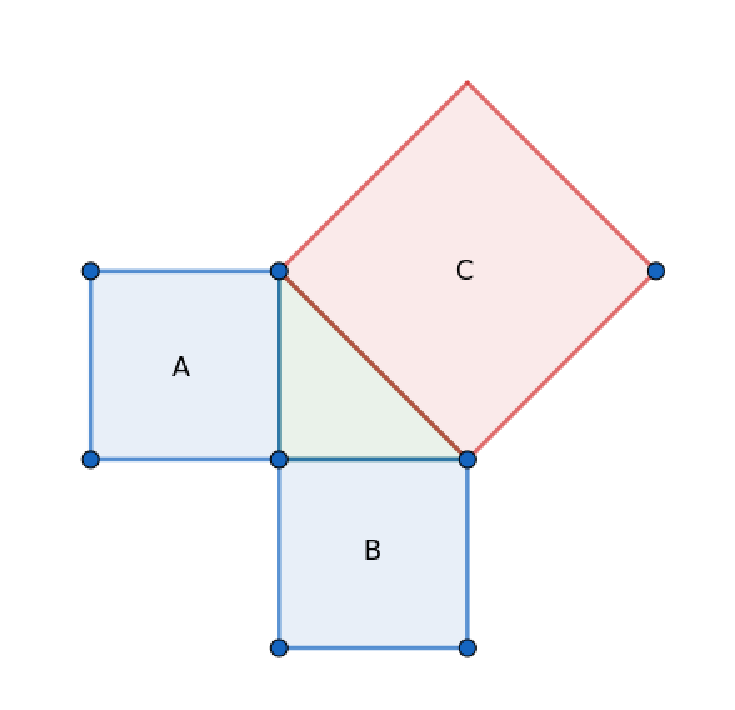
\includegraphics[scale=0.5]{images/thm_pitagoras}
   \caption{El teorema de Pitágoras.}
   \label{fig:pitagoras}
\end{figure}

\begin{exercise}
	Demuestre el teorema de Pitágoras utilizando el diagrama de la
	figura~\ref{fig:pitagoras1}.
	\begin{figure}[h]
		\centering
		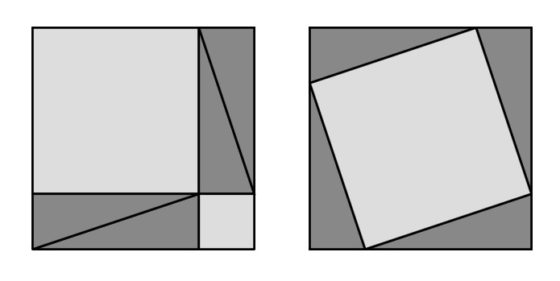
\includegraphics[scale=.4]{images/pitagoras_proof}
		\caption{Otra demostración del teorema de Pitágoras, en general
		atribuida a la matemática china.}
		\label{fig:pitagoras1}
	\end{figure}
\end{exercise}

\begin{exercise}
	Utilice la figura~\ref{fig:semejanza} y 
	demuestre el teorema de Pitágoras.
	\begin{figure}[h]
		\centering
		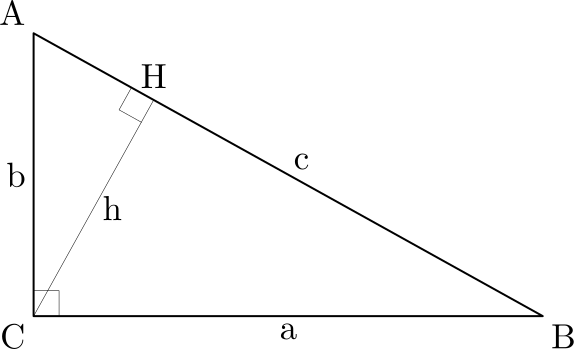
\includegraphics[scale=.2]{images/pitagoras_semejanza}
		\caption{Otra demostración del teorema de Pitágoras.}
		\label{fig:semejanza}
	\end{figure}
\end{exercise}

\begin{exercise}
	Utilice la figura~\ref{fig:Bhaskara} y 
	demuestre el teorema de Pitágoras.
	\begin{figure}[h]
		\centering
		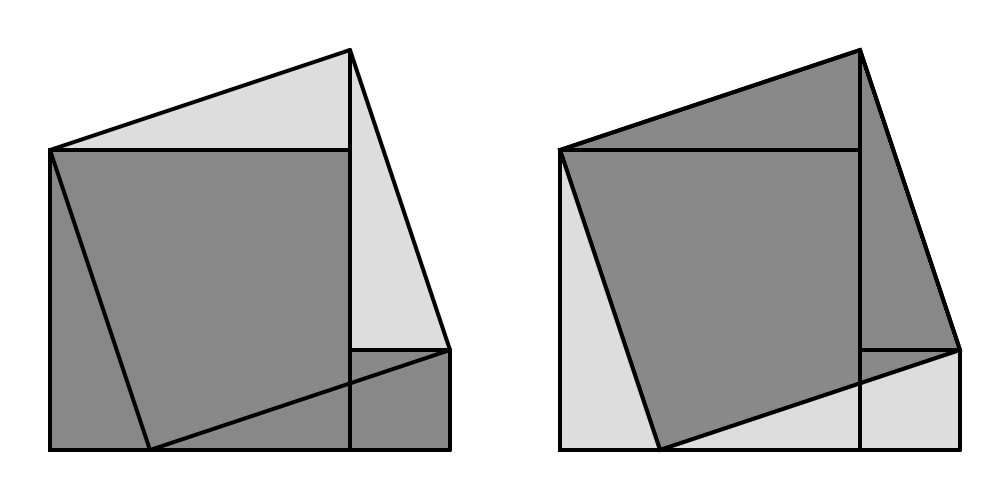
\includegraphics[scale=.2]{images/pitagoras_bhaskara}
		\caption{Otra demostración del teorema de Pitágoras, en general
		atribuida al matemático indio Bhaskara.}
		\label{fig:Bhaskara}
	\end{figure}
\end{exercise}


\begin{exercise}
	Utilice la figura~\ref{fig:arabe} y 
	demuestre el teorema de Pitágoras.
	\begin{figure}[h]
		\centering
		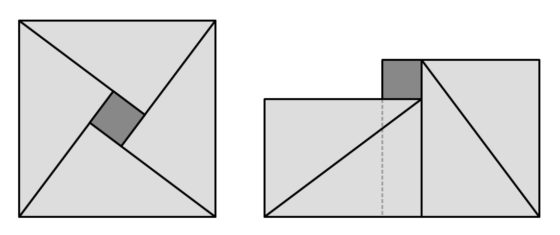
\includegraphics[scale=.5]{images/pitagoras_arabe}
		\caption{Otra demostración del teorema de Pitágoras, en general
		atribuida al matemático árabe Thabit ibn Qurrá.}
		\label{fig:arabe}
	\end{figure}
\end{exercise}

\begin{exercise}
	\index{Zhoubi Suanjing}
	Uno de los textos más antiguos de matemática china es el Zhoubi Suanjing,
	que data del período de la dinastía Zhou. Allí aparece una de las primeras
	demostraciones escritas del teorema de Pitágoras, basada en la
	figura~\ref{fig:China}. ¿Cómo puede usarse esa figura para demostrar el
	teorema de Pitágoras?
	\begin{figure}[h]
		\centering
		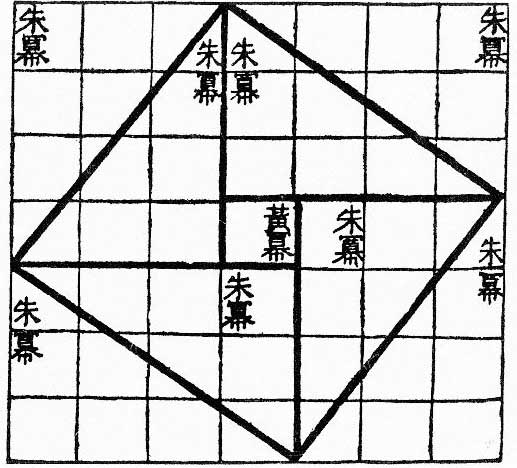
\includegraphics[scale=0.2]{images/pitagoras_china}
		\caption{Una demostración del teorema de Pitágoras.}
		\label{fig:China}
	\end{figure}
\end{exercise}

\begin{exercise}
	En los elementos de Euclides aparece una demostración del teorema de
	Pitágoras. ¿Cuál es esa demostración? ¿Aparecen otras demostraciones del
	teorema de Pitágoras en estos famosos libros de Euclides?
\end{exercise}

\begin{exercise}
	Existe una demostración del teorema de Pitagóras que se le atribuye a
	Leonardo Da Vinci. ¿Cuál es esa demostración?
\end{exercise}

\begin{exercise}
	La demostración del teorema de Pitágoras de este ejercicio fue descubierta
	por Garfield, el vigésimo Presidente de los Estados Unidos.  Demuestre el
	teorema de Pitágoras utilizando la figura~\ref{fig:garfield}.
	\begin{figure}[h]
		\centering
		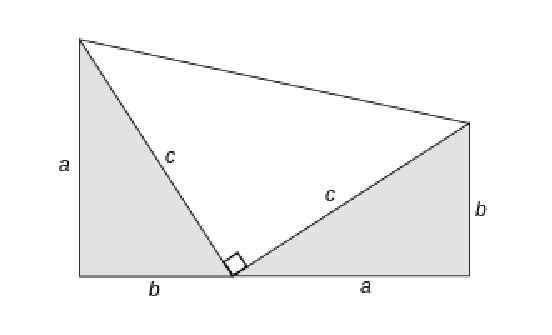
\includegraphics[scale=0.5]{images/garfield}
		\caption{La demostración de Garfield del teorema de Pitágoras.}
		\label{fig:garfield}
	\end{figure}
\end{exercise}


El teorema de Pitágoras sugiere sutilmente que existe una profunda relación
entre la aritmética y la geometría. Esta relación entre aritmética y geometría
es también fundamental en el desarollo de las matemáticas. 

Se cree que en tiempos antiguos se usaban distintas soluciones de la ecuación
del teorema de Pitágoras para construir ángulos rectos.  Por ejemplo, con una
cuerda con doce nudos equidistantes (es decir, una cuerda de ``longitud'' igual
a doce), se lograba construir el triángulo rectángulo $(3,4,5)$.  Hoy en día
usamos el teorema de Pitágoras para calcular longitudes y distancias.  Si
$A=(a_1,a_2)$ y $B=(b_1,b_2)$ son dos puntos del plano cartesiano, se define la
distancia entre $A$ y $B$ como 
\[
	\dist(A,B)=\sqrt{(a_1-b_1)^2+(a_2-b_2)^2}.
\]
Esta fórmula para calcular la distancia entre dos puntos del plano puede
extenderse fácilmente a puntos de un espacio de dimensión finita arbitraria. 

Se tiene
además una generalización del teorema de Pitágoras a espacios vectoriales de
dimensión finita: Si $V$ es un espacio vectorial con producto interno y
$v_1,\dots,v_n\in V$ son vectores ortogonales dos a dos, entonces 
\[
	\|v_1+\cdots+v_n\|^2=\sum_{i=1}^n \|v_i\|^2.
\]
Se recupera el teorema de Pitágoras al tomar $V=\R^2$ con el producto interno
usual.
%\[
%	\langle (x_1,y_1),(x_2,y_2)\rangle=x_1x_2+y_1y_2.
%\]

\begin{figure}[h]
	\centering
	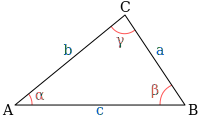
\includegraphics[scale=.5]{images/coseno}
	\caption{El teorema del coseno.}
	\label{fig:coseno}
\end{figure}

El teorema de Pitágoras puede verse como un caso particular del \textbf{teorema
del coseno}, que afirma que en un triángulo como el que vemos en la
figura~\ref{fig:coseno}, se tiene $c^2=a^2+b^2-2ab\cos\gamma$.

\begin{exercise}
	Demuestre el teorema del coseno.
\end{exercise}

Con el teorema del coseno podemos demostrar un lindo resultado publicado por el
matemático escocés Matthew Stewart en 1746: Si se tiene un triángulo como el
que vemos en la figura~\ref{fig:Stewart}, entonces
\[
	mb^2+nc^2=mn^2+nm^2+ad^2.
\]

\begin{figure}[h]
	\centering
	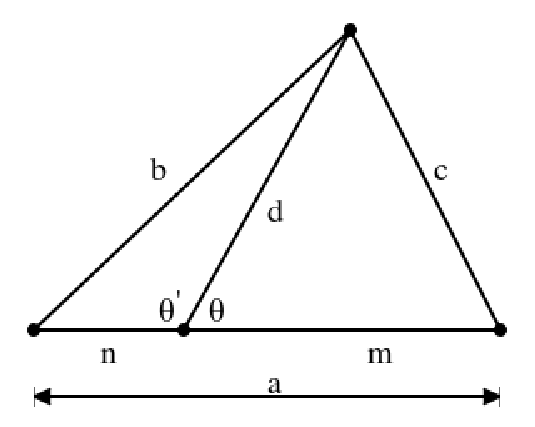
\includegraphics[scale=.4]{images/stewart}
	\caption{El teorema de Stewart.}
	\label{fig:Stewart}
\end{figure}

Aparentemente Stewart publicó este resultado en 1746 cuando era candidato a
reemplazar a Maclaurin como profesor de la Universidad de Edimburgo.  Se cree
que Arquímedes conocía ya este resultado. De hecho, el teorema de Stewart es
una generalización del teorema de las medianas de Apolonio, que afirma 
que en el triángulo de la figura~\ref{fig:Stewart} se tiene
\[
	b^2+c^2=\frac12a^2+2d^2.
\]

\begin{exercise}
	Demuestre el teorema de Stewart.
\end{exercise}

\begin{exercise}
	Demuestre el teorema de las medianas de Apolonio.
\end{exercise}

\section*{Ternas pitagóricas}
\index{Ternas pitagóricas}

Nos proponemos ahora encontrar ternas pitagóricas, es decir ternas
$(a,b,c)\in\N^3$ tales que $a^2+b^2=c^2$.  Para más información sobre aspectos
históricos sobre la construcción de ternas pitagóricas conviene mirar el
segundo volumen del tratado de Dickson sobre la historia de la teoría de
números~\cite{MR0245500}. 

\begin{exercise}
	Si $(a,b,c)$ es una terna pitagórica, entonces $(ka,kb,kc)$
	es una terna pitagórica.
\end{exercise}

\index{Terna pitagórica!primitiva}
Un ejemplo fácil de terna
pitagórica es $(3,4,5)$. 
Otro ejemplo de terna pitagórica es $(6,8,10)$, aunque podríamos acusarlo de no
es muy interesante pues puede obtenerse como 
\[
(6,8,10)=2\times (3,4,5). 
\]
Nos interesan entonces las ternas pitagóricas
\textbf{primitivas}, es decir las ternas pitagóricas $(a,b,c)$ con $a$, $b$ y $c$
coprimos. Veamos otros ejemplos de ternas pitagóricas primitivas:
\begin{align*}
	(5,12,13), &&
	(8,15,17), &&
	(7,24,25), && 
	(20,21,29),&&
	(12,35,37), \\
	(9,40,41), &&
	(28,45,53),&&
	(11,60,61),&&
	(16, 63, 65),&&
	(33, 56, 65),\\
	(48, 55, 73),&&
	(13, 84, 85),&&
	(36, 77, 85),&&
	(39, 80, 89),&&
	(65, 72, 97).
\end{align*}

Si bien Pitágoras vivió alrededor del 500 a. C., las ternas pitagóricas se
conocen desde mucho antes. Se sabe que las ternas pitagóricas fueron de interés
en Babilonia, en China y en India, se cree que para la construccción de ángulos
rectos.  Una de las referencias más antiguas a las ternas pitagóricas es una
tabla babilónica de arcilla conocida como Plimpton 322. Se cree que esta tabla
fue escrita en el año 1800 a. C. El nombre se debe al siguiente hecho: a
comienzos del siglo XX un editor llamado George Arthur Plimpton compró aquella
tabla de barro y tiempo después la entregó a la Universidad de Columbia; esta
tabla es la número 322 de la colección que Plimpton cedió a la Universidad de
Columbia.  Existen diversas interpretaciones sobre qué información contiene
esta tabla y cómo fue que los babilónicos pudieron calcularla. 

%Consideremos la figura\dots 
%Claramente tenemos $BC=AD$. Si $a+b$ es el lado $AC$, entonces $DB=a-b$. 
%Observemos además que
%\[
%	AO=OC=\frac12(a+b),\quad
%	DO=OB=\frac12(a-b)
%\]
%y entonces $AB=AO+OB$ y $AD=AO-OD$. Si elevamos al cuadrado, 
%\[
%	(a+b)^2=AE,\quad
%	(a-b)^2=FG
%

Un estudio reciente revela que la tabla describe las formas del triángulo
rectángulo usando una novedosa forma de trigonometría; para más información
referimos a~\cite{MR3716328}.

\begin{figure}
   \centering
   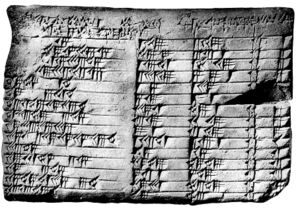
\includegraphics[scale=0.8]{images/plimpton322}
   \caption{La tabla Plimpton 322.}
   \label{fig:plimpton}
\end{figure}


Según Proclo, Pitágoras conocía la regla 
\[
	x=2\alpha+1,\quad
	y=2\alpha^2+2\alpha,\quad
	z=y+1,
\]
para generar ternas pitagóricas. Platón conocía la regla 
\[
	x=2\alpha,\quad
	y=\alpha^2-1,\quad
	z=\alpha^2+1.
\]
En sus elementos, en la proposición 5 del libro II, Euclides dio la regla 
\[
		x=\alpha\beta\gamma,
		\quad
		y=\frac12\alpha(\beta^2-\gamma^2),
		\quad
		z=\frac12\alpha(\beta^2+\gamma^2),
\]
para construir ternas pitagóricas.  En la proposición 30 del libro X, dio otra
regla:
\[
		x=\sqrt{mn},\quad
		y=\frac12(m-n),\quad
		z=\frac12(m+n).
\]
Al menos un siglo antes que Diofanto, Nipsus dio la siguiente regla: 
\begin{align*}
	&z=\frac12(x^2+1), && y=\frac12(x^2-1), &&\text{si $x$ es impar},\\
	&z=\frac14x^2+1, && y=\frac14x^2-1, &&\text{si $x$ es par},
\end{align*}
y además $x^2=z^2-y^2$. Estas fórmulas son equivalentes a las fórmulas dadas
por Pitágoras y Platón. Más tarde, Diofanto presentó un ingenioso método
geométrico que le permitió obtener las siguientes fórmulas 
\begin{equation}
	\label{eq:formula}
	a=(p^2-q^2)r,\quad
	b=2pqr,\quad
	c=(p^2+q^2)r,
\end{equation}
para generar ternas pitagóricas. 

Los babilónicos no disponía de notación algebraica, pero se cree que 
conocían  
las fórmulas~\eqref{eq:formula} en el caso $r=1$ y que así fue como lograron
listar ternas pitagóricas. Las fórmulas~\eqref{eq:formula} como método para
obtener ternas pitagóricas aparece también en la matemática india y en
manuscritos árabes. 
%En forma independiente, Brahmagupta, que nació en el año 598, dio esa misma
%fórmula para generar ternas pitagóricas. Un manuscrito árabe anónimo del año
%972 afirma que~\eqref{eq:formula} permite obtener todas las soluciones de la
%ecuación pitagórica. En el siglo X, Alhocain dio una demostración geométrica
%de la fórmula~\eqref{eq:formula}. 
En 1738 Koerbero demostró que la fórmula~\eqref{eq:formula} permite obtener
todas las soluciones. Kronecker demostró en 1901 que la
fórmula~\eqref{eq:formula} no solamente da todas las soluciones sino que esto
se hace sin repeticiones si $p>q>0$ y $r>0$. 

Que las fórmulas~\eqref{eq:formula} produzcan ternas pitagóricas es un caso
particular de la siguiente identidad que involucra sumas de dos cuadrados:
\begin{equation}
	\label{eq:2cuadrados}
	(x_1x_2-y_1y_2)^2+(x_1y_2+x_2y_1)^2=(x_1^2+y_1^2)(x_2^2+y_2^2).
\end{equation}
Esta identidad era ya conocida por Diofanto, que la interpretó como una regla
para generar triángulos rectángulos: si se tienen dos triángulos rectángulos de
lados $(x_1,y_1)$ y $(x_2,y_2)$, entonces puede construirse un triángulo
rectángulo de lados $(x_1x_2-y_1y_2, x_1y_2+x_2y_1)$.  
%En 1593 Vieta observó
%que 
%\[
%	\frac{x_2y_1+x_1y_2}{x_1x_2-y_1y_2}=\frac{\frac{y_1}{x_1}+\frac{y_2}{x_2}}{1-\frac{y_1}{x_1}\frac{y_2}{x_2}}=\tan(\theta_1+\theta_2),
%\]
%donde $\tan(\theta_1)=y_1/x_1$ y $\tan(\theta_2)=y_2/x_2$.  

\begin{exercise}
Demuestre la identidad~\eqref{eq:2cuadrados}. 
\end{exercise}

%Gauss fue una de los primeros matemáticos en considerar seriamente
%``composiciones de sumas de cuadrados''. 

Encontrar ternas pitagóricas es en realidad
encontrar soluciones enteras a una cierta ecuación.  
%Una demostración
%puramente aritmética de la fórmula general~\eqref{eq:formula} fue dada por
%Euclides. 
% ver conrad
% http://www.math.uconn.edu/~kconrad/blurbs/ugradnumthy/pythagtriple.pdf

\begin{exercise}
	\label{xca:paridad}
	Demuestre que si $(a,b,c)$ es una terna pitagórica primitiva, entonces $a\equiv b+1\bmod
	2$. 
\end{exercise}

% Como $(a,b,c)$ es primitiva, $a$ y $b$ no pueden ser ambos números pares. 
% Si $a$ y $b$ son ambos impares, $a^2\equiv b^2\equiv1\bmod4$ y luego
% $a^2+b^2\equiv 2\bmod4$, que no es un cuadrado módulo cuatro. 

\begin{theorem}
	\label{thm:ternas_pitagoricas}
	Sea $(a,b,c)$ una terna pitagórica primitiva tal que $b$ es un número par.
	Entonces 
	\[
		a=m^2-n^2,\quad
		b=2mn,\quad
		c=m^2+n^2
	\]
	para ciertos enteros coprimos $m,n$ tales que $m>n>0$ y $m\not\equiv n\bmod
	2$. Recíprocamente todas las ternas de esa forma son ternas pitagóricas
	primitivas. 
\end{theorem}

\begin{proof}
	Como $b$ es par, $a$ es impar y luego $c^2=a^2+b^2$ es también impar. Escribimos
	\[
		b^2=c^2-a^2=(c+a)(c-a). 
	\]
	Los números $c+a$ y $c-a$ son ambos pares. Al dividir por
	cuatro podemos reescribir $b^2=(c+a)(c-a)$ como 
	\[
		\left(\frac{b}{2}\right)^2=\frac{c+a}{2}\frac{c-a}{2}.
	\]
	Observemos que $\frac{c+a}{2}$ y $\frac{c-a}{2}$ son coprimos pues si $d$
	es un divisor común, entonces $d=1$ pues $d$ divide al número 
	$c=\frac{c-a}{2}+\frac{c+a}{2}$ y también al número 
	$a=\frac{c-a}{2}-\frac{c+a}{2}$. Por el teorema de factorización única
	sabemos que existen enteros coprimos $m,n$ tales que
	\[
		\frac{c+a}{2}=m^2,\quad
		\frac{c-a}{2}=n^2.
	\]
	Al despejar obtenemos entonces que 
	\[
		c=m^2+n^2,\quad
		a=m^2-n^2
	\]
	y luego $b=2mn$ tal como queríamos demostrar. 
	
	Como $m$ y $n$ son coprimos,
	no pueden ser ambos números pares. Si ambos fueran impares, los números
	$m^2+n^2$, $2mn$ y $m^2-n^2$ serían pares, una contradicción pues $(a,b,c)$
	es una terna primitiva.
\end{proof}

Veamos una explicación geométrica de las fórmulas de Euclides que utiliza las
ideas de Diofanto. Utilizaremos nuestro lenguaje algebraico, ya que esto
facilitará mucho las cuentas.  Primero escribamos $a^2+b^2=c^2$ como
\[
	\left(a/c\right)^2+\left(b/c\right)^2=1.
\]
Si $x=a/c$, $y=b/c$, el problema entonces es encontrar soluciones racionales de 
la ecuación 
\begin{equation}
\label{eq:circulo}
	x^2+y^2=1.
\end{equation}
Como sabemos, esta es la ecuación del círculo con centro en $(0,0)$ y radio
$1$.  Sea $P=(x,y)$ una solución racional de la ecuación \eqref{eq:circulo}, 
podemos tomar por
ejemplo $(x,y)=(-1,0)$. Si $L$ es la recta con pendiente racional $t$ que pasa
por $P$, $y=t(x+1)$, entonces $L$ corta al círculo $x^2+y^2=1$ en un punto $Q$
que también tiene coordenadas racionales. Al reemplazar $y=t(m+1)$ en
$x^2+y^2=1$ y utilizar que la ecuación cuadrática
\[
	x^2+t^2(x+1)^2=1
\]
tiene como solución $x=-1$, se obtiene que la otra solución es también un
número racional. Como la segunda solución de esta cuadrática es
\[
	x=\frac{1-t^2}{1+t^2},
\]
se concluye que 
\[
	y=\frac{2t}{1+t^2}.
\]

De estas expresiones es fácil obtener la fórmula general para encontrar ternas
pitagóricas que mencionamos anteriormente. 

Es muy importante remarcar el siguiente hecho notable: encontrar ternas
pitagóricas es entonces encontrar soluciones racionales de una cierta ecuación, 
es decir, encontrar los puntos racionales de una cierta curva. 

%\subsubsection*{Construcción de ternas pitagóricas}
%Veamos cómo construir ternas pitagóricas primitivas. Sean 
%\[
%	A_1=\begin{pmatrix}
%		-1 & 2 & 2\\
%		-2 & 1 & 2\\
%		-2 & 2 & 3
%	\end{pmatrix},
%	\quad
%	A_2=\begin{pmatrix}
%		1 & 2 & 2\\
%		2 & 1 & 2\\
%		2 & 2 & 3
%	\end{pmatrix},
%	\quad
%	A_3=\begin{pmatrix}
%		1 & -2 & 2\\
%		2 & -1 & 2\\
%		2 & -2 & 3
%	\end{pmatrix}.
%\]
%Toda terna pitagórica primitiva $(a,b,c)$ 
%puede obtenerse como 
%\begin{equation}
%	\label{eq:pitagoras}
%	\colvec{3}{a}{b}{c}=A_{i_1}\cdots A_{i_k}\colvec{3}{3}{4}{5}
%\end{equation}
%para algunos enteros $i_1,\dots,i_k\in\{1,2,3\}$. Veamos que toda terna pitagórica primitiva puede
%obtenerse mediante la fórmula~\eqref{eq:pitagoras}. Si $m$ y $n$ son enteros
%coprimos tales que $m>n$ y $m=n+1\bmod 2$, entonces para obtener la terna 
%\[
%	(m^2-n^2,2mn,m^2+n^2)
%\]
%hay tres casos a considerar. 
%\begin{itemize}
%	\item Si $n<m<2n$, entonces sean $s=n$ y $t=2n-m$, es decir $n=s$ y $m=2s-t$. 
%	\item Si $2n<m<3n$, entonces sean $s=$\dots
%	\item Si $3n<m$, entonces sean $\dots$.
%\end{itemize}
%En los tres casos anteriores $s$ y $t$ son números coprimos de distinta paridad
%y tales que $t>s$ y $s+t<m+n$. 
%
%Dickson encontró un método que permite construir todas las ternas pitagóricas.
%El método funciona de la siguiente forma: si $r,s,t$ son enteros positivos,
%entonces la terna $(r+s,r+t,r+s+t)$ es pitagórica si $r^2=2st$.
%
%\begin{theorem}[Dickson]
%	Sean $k,p,q$ enteros tales que $k>q$ y sean $c=k+p$, $b=p+q$ y $a=k$.
%	Entonces $a^2+b^2=c^2$ si y sólo si $q^2=2p(k-q)$.
%\end{theorem}
%
%\begin{proof}
%	Vamos a encontrar una biyección entre $(k,q,p)$ y $(a,b,c)$ 
%\end{proof}
%
%
%
%%Veamos ahora una explicación que usa álgebra lineal. Dados $a,b,c\in\N$ sea
%%\[
%%	X=\begin{pmatrix}
%%		c+b & a\\
%%		a & c-b
%%	\end{pmatrix}.
%%\]
%%Es claro que $X$ es una matriz sim\'etrica, es decir $X=X^T$. Además
%%$\det(X)=c^2-b^2-a^2$. Luego $X=0$ si y sólo si $(a,b,c)$ es una terna
%%pitagórica. Más aún, si $(a,b,c)$ es una terna pitagórica, el rango de $X$ es
%%igual a uno. 
%

\section*{Los babilónicos}

Es un buen momento para hacer una pequeña digresión y hablar sobre la
matemática de los babilónicos.  Hasta principios del siglo XX poco se sabía
sobre la matemática de los pueblos que habitaban la mesopotamia, sumerios,
acadios, babilonios, asirios. Hacia el año 3000 a. C. los sumerios introdujeron
un sistema de numeración posicional de base 60, que es esencialmente el sistema
sexagesimal que aún hoy utilizamos en las mediciones de tiempo y ángulos. La
inexistencia de un símbolo para el cero y de un signo que permitiera
diferenciar parte entera y parte fraccionaria, hace que el sistema de
numeración de los sumerios resulte impreciso para nuestros ojos, aunque los
sumerios lo utilizaban hábilmente, ya sea mediante el uso de símbolos
auxiliares que permitieran evitar ambigüedades o simplemente gracias al
contexto en el que se encontraba un determinado problema. 

A principios del siglo XX se encontraron textos pertenecientes al período
babilónico, digamos del año 2000 a. C., donde se da cuenta de los conocimientos
matemáticos que los sumerios tenían alrededor del año 3000 a. C. y una
colección de problemas numéricos particulares junto con sus soluciones. Entre
estos aportes vemos cómo los babilónicos resolvían ecuaciones lineales y
cuadráticas. 
En uno de los problemas se plantea un problema cuya solución depende de resolver
el sistema lineal
\begin{align*}
	x+y &= 1800,\\
	(2/3)x-(1/2)y&=500.
\end{align*}
La solución depende de la introducción de una nueva variable $z$ tal que
\begin{align*}
x&=900+z,\\
y&=900-z.     
\end{align*}
Al reemplazar estas fórmulas en la segunda ecuación del
sistema puede obtenerse el valor de $z$, que nos da al par $(x,y)=(1200,600)$
como única solución del sistema. 

En otro problema se plantea un problema que requiere resolver 
\begin{align*}
	xy+x-y &= 183,\\
	x+y&=27.
\end{align*}
Para resolver este problema se observa que el sistema puede reescribirse como 
\begin{align*}
	x(y+2)&=210,\\
	x+(y+2)&=29
\end{align*}
y luego se encuentran los números cuya suma es 29 y su producto es 210 de forma
más o menos similar a la que usaríamos hoy en día.

Aparece además un problema de interés compuesto que requiere resolver la
ecuación que hoy escribimos como
\[
	(5/6)^x=2.
\]
La solución de esta ecuación se obtiene en forma aproximada mediante un método
que no es sino una forma precaria del método ``regula falsi'' que hoy en día
podemos encontrarnos en casi cualquier curso de cálculo numérico.

Nos encontramos al teorema de Pitágoras como método para calcular raíces
cuadradas; esto se hace en forma aproximada y mediante la fórmula
\[
	\sqrt{n}=\sqrt{a^2\pm r}\sim a\pm \frac{r}{2a}.
\]
Para calcular el área de un círculo de circunferencia $c$, los babilónicos lo
hacían aproximadamente gracias a la fórmula $c^2/12$.  Como aceptaban que el
triple del diámetro es igual a la circunferencia, tenían que el área de un
círculo de radio $r$ es aproximadamente igual a $3r^2$. 

Podían realizar cálculos relacionados con segmentos circulares tal como el que
vemos en la figura~\ref{fig:circular}. Sabían, por ejemplo, que
\[
	h=R-\sqrt{R^2-(c/2)^2}
\]
y tenían una fórmula para calcular el valor del segmento $c$.  

\begin{figure}
   \centering
   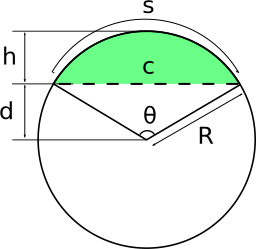
\includegraphics[scale=0.4]{images/circular}
   \caption{Un segmento circular.}
   \label{fig:circular}
\end{figure}

Podría decirse que estos son los primeros pasos de la trigonometría,
desarrollada mucho después por el matemático griego Hiparco.  Los babilonios no
desarrollaron la noción de ángulo, solamente aparecen en los documentos
implícitamente los triángulos rectángulos. 

De los textos encontrados resulta evidente que los babilónicos conocían la
proporcionalidad entre los lados de triángulos semejantes, sabían cómo calcular
áreas de triángulos y trapecios y volúmenes de prismas y cilindros. Los textos
nos muestran que los babilónicos disponían de una técnica medio geométrica y
medio algebraica, que les permitió manipular eficientemente ecuaciones lineales
y cuadráticas. Esta técnica es muy similar a la que nos encontraremos en uno de
los libros de Euclides, escrito aproximadamente en el año 300 a. C.
Intentaremos describir brevemente esta técnica de los babilónicos y para esto
seguiremos la presentación del primer volumen del tratado de Babini y Rey
Pastor~\cite{BabiniReyPastor1,BabiniReyPastor2}.  Supongamos que se tiene un
cuadrado como el que vemos en la figura~\ref{fig:babilonios}. 
\begin{figure}
   \centering
   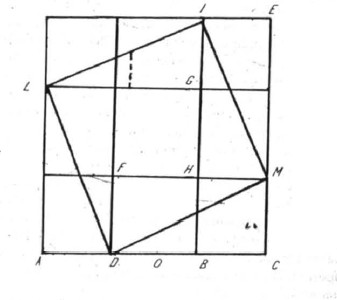
\includegraphics[scale=0.4]{images/babilonios}
   \caption{La técnica de los babilónicos.}
   \label{fig:babilonios}
\end{figure}
Si el segmento AB mide $a$ y AD mide $b$, entonces AC mide $a+b$ y BD mide
$a-b$. Si O es el centro de simetría del segmento AC, entonces AO y OC son
ambos iguales a $\frac12(a+b)$ y además DO y OB son ambos iguales a
$\frac12(a-b)$. El cuadrado de la figura~\ref{fig:babilonios} puede
descomponerse en cuadrados y rectángulos y de estas descomposiciones podemos
obtener las siguientes fórmulas:
\begin{align*}
	(a+b)^2 &= a^2+b^2+2ab,\\
	(a-b)^2+2ab &= a^2 + b^2,\\
	(a+b)(a-b) &= a^2-b^2,\\
	(a+b)^2 &= 4ab+(a-b)^2,
\end{align*}
fórmulas que los babilónicos usaron en la resolución de problemas. Si $c$ es la medida de la hipotenusa del triángulo
DCM, entonces obtenemos también que 
\[
	c^2\pm 2ab=(a\pm b)^2,
\]
fórmula que no es otra cosa sino una versión del teorema de Pitágoras. La
fórmula $(a+b)^2=(a-b)^2+4ab$ nos lleva casi inmediatamente a la regla de
construcción de ternas pitagóricas que mencionamos anteriormente: simplemente
debemos tomar $a=m^2$, $b=n^2$ y luego 
\[
	(m^2-n^2)^2+(2mn)^2=(m^2+n^2)^2.
\]



\chapter{Números irracionales}

¿Por qué es tan importante el teorema de Pitágoras?  El teorema 
introduce naturalmente números irracionales. La hipotenusa de un triángulo
rectángulo cuyos lados miden uno es igual a $\sqrt{2}$, un número cuyo cuadrado
es dos.  En tiempos de Pitágoras esto se mantuvo en secreto ya que no era un
resultado que pudiera comprenderse totalmente. Los pitagóricos
no podían aceptar que $\sqrt{2}$ fuera un número, aunque supieran que $\sqrt{2}$ es
la diagonal de un cuadrado unitario. Las cantidades geométricas
eran entonces, en general, tratadas de forma que no fuera necesario utilizar números. La
relación entre aritmética y geometría estaba parcialmente rota. Sin embargo,
para solventar las dificultades originadas por esta división, los griegos
desarrollaron entonces ingeniosos métodos para entender cuánto podría
aproximarse una cierta cantidad geométrica en términos de números racionales.
Podemos encontrar estas ideas en el libro X de los Elementos, donde Euclides
estudia detalladamente números de la forma
\[
	\sqrt{\sqrt{a}\pm\sqrt{b}}
\]
donde $a$ y $b$ son números racionales. 

Durante muchos años la matemática no vio avances en relación con los números
irracionales, salvo, quizá, la observación que hizo Fibonacci en 1225 sobre la
irracionalidad de las soluciones de la ecuación 
\[
	x^3+2x^2+10x=20.
\]
Fibonacci demostró que las soluciones son números irracionales, pero no esos
irracionales estudiados por Euclides en el libro X. 

Las ideas sobre irracionales de la matemática griega fueron redescubiertas por
Dedekind en el siglo XIX y permitieron que la aritmética y la geometría
finalmente pudieran convivir pacíficamente.

\begin{exercise}
	Demuestre que un entero $m$ es par si y sólo si $m^2$ es par.
\end{exercise}

La demostración de la irracionalidad de $\sqrt{2}$ que daremos a continuación
aparece en uno de los libros de Aristóteles.

\begin{theorem}
	El número $\sqrt{2}$ no es racional.	
\end{theorem}

\begin{proof}
	Si suponemos que $\sqrt{2}=a/b$ con $a$ y $b$ son números naturales sin
	factores en común, entonces $(a/b)^2=2$. Esto implica que $a^2=2b^2$ es un
	número par. Luego $a$ es par, digamos $a=2c$. Entonces $2b^2=a^2=4c^2$
	implica que $b^2=2c^2$ y luego $b$ es par, una contradicción.
\end{proof}

% agregar los ejercicios del libro de rey pastor y Babibi
% ver si hay algo interesante en stillwell
La demostración que vimos usa fuertemente la paridad de los números naturales.
Gracias a uno de los diálogos de Platón sabemos que el matemático griego
Teodoro estudió algunos números irracionales y demostró la irracionalidad de
$\sqrt{n}$ para los $n<17$ que no son cuadrados. Se nos dice además que Teodoro
concibió la figura~\ref{fig:teodoro} y que justamente fue en el número 17 donde
su análisis se detuvo. 

\begin{figure}[h]
		\centering
		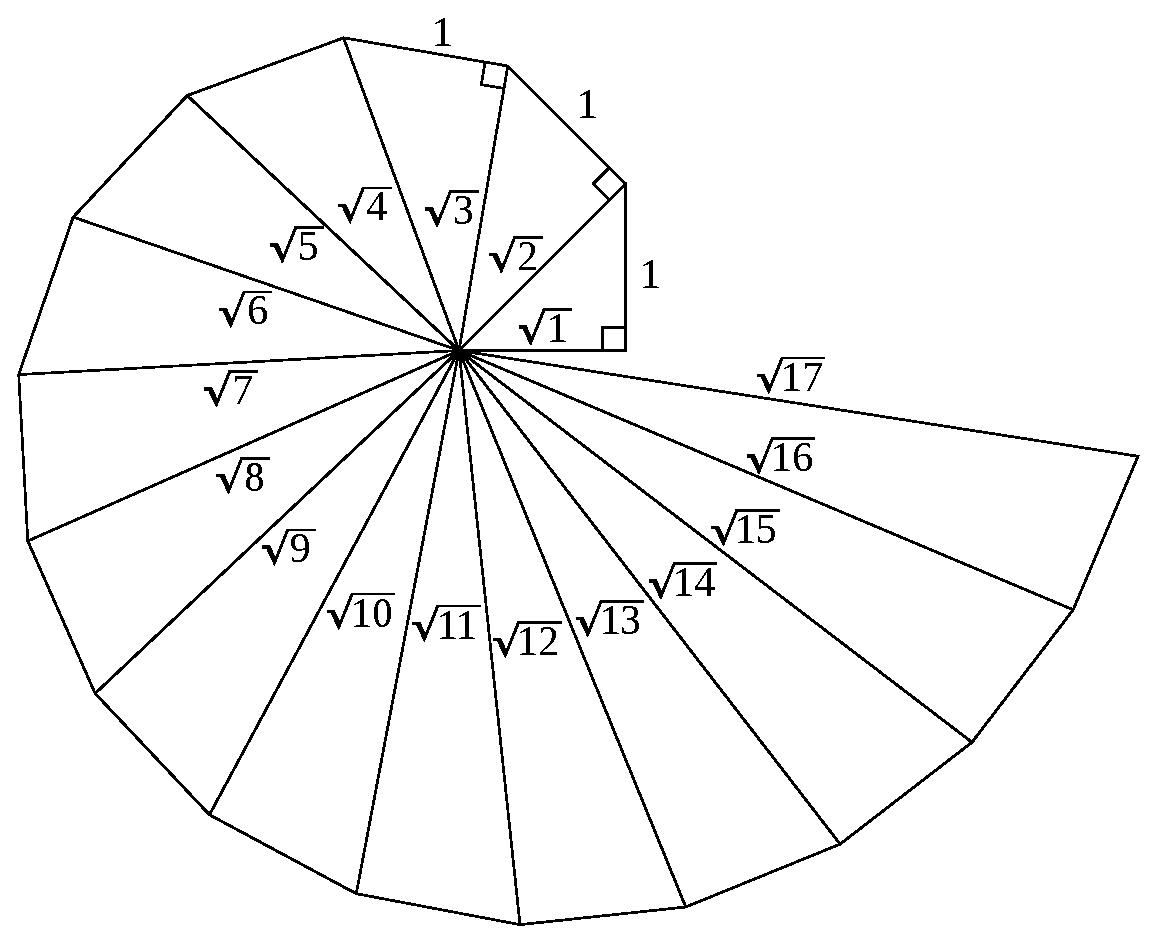
\includegraphics[scale=0.3]{images/teodoro}
		\caption{La espiral de Teodoro.}
		\label{fig:teodoro}
\end{figure}

No se sabe exactamente qué demostraciones encontró
Teodoro. Más interesante fue para los historiadores saber por qué Teodoro se
detuvo justamente en $17$. Algunos creen que fue porque a partir de ese número
el dibujo que vemos en la figura~\ref{fig:teodoro} tiene superposiciones, aunque
esta versión no parece ser una explicación suficientemente fuerte 
como para convencernos. De hecho, en 1958 se demostró que esas supuestas superposiciones 
son fácilmente evitables si extendemos la espiral tal como vemos en la
figura~\ref{fig:espiral_infinita}.  

\begin{figure}[h]
		\centering
		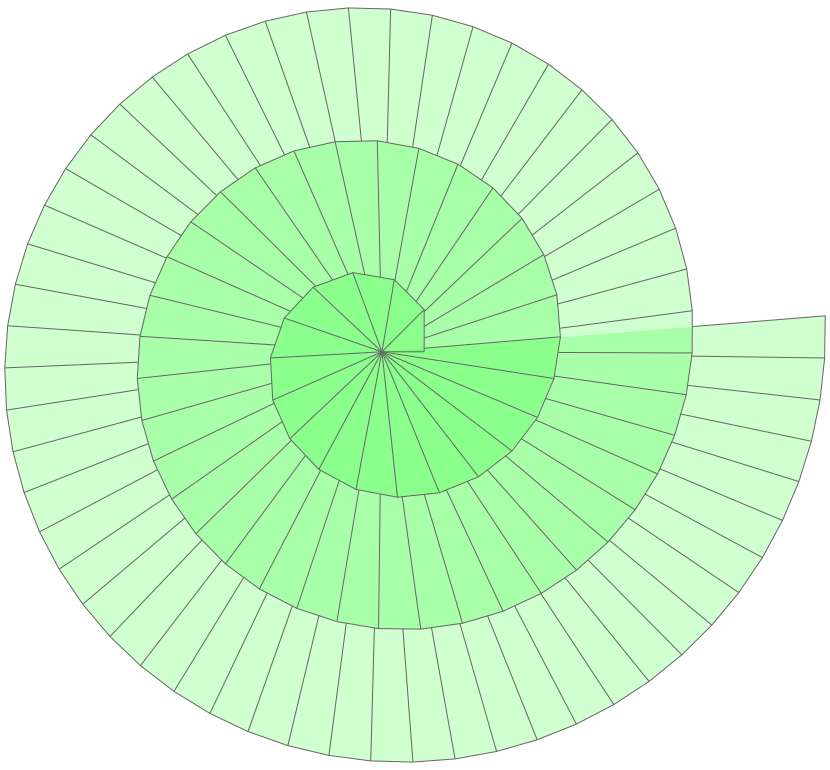
\includegraphics[scale=0.2]{images/infinita}
		\caption{Una extensión de la espiral de Teodoro.}
		\label{fig:espiral_infinita}
\end{figure}

Una explicación más razonable --observada
por Heath en 1931-- se basa en el siguiente hecho: la técnica basada en el uso
de la paridad falla por primera vez justamente en 17.  Supongamos que
$\sqrt{17}=a/b$, donde $a$ y $b$ son coprimos; entonces $17b^2=a^2$. Como $a$ y
$b$ son coprimos, ambos son impares, digamos $a=2k+1$ y $b=2l+1$. Al reemplazar
obtenemos entonces
\[
	17(4l^2+4l+1)=4k^2+4k+1,
\]
que al simplificarse queda $17l(l+1)+4=k(k+1)$. ¡Aquí no hay contradicción!

Tal como se afirma en~\cite{MR0416824}, muy probablemente esta sea la razón por
la que Teodoro detuvo su análisis en 17. No nos olvidemos que los griegos
creían fuertemente en la potencia de las técnicas de paridad. De hecho, para
Platón la aritmética era la teoría de los pares y los impares. 

Veamos ahora que el argumento de paridad sí funciona para números menores que
17 que no son cuadrados. Este resultado será consecuencia de un resultado mucho
más general:

\begin{theorem}
	Si $n$ es un entero positivo que puede escribirse como $4m+2$, $4m+3$,
	$8m+5$, entonces puede demostrarse que $\sqrt{n}$ es irracional con un
	argumento de paridad.
\end{theorem}

\begin{proof}
	Consideremos el caso $n=8m+5$ y escribamos $\sqrt{8m+5}=a/b$, donde $a$ y
	$b$ son coprimos. Como $(8m+5)b^2=a^2$, tanto $a$ como $b$ deberán ser
	números impares. Escribimos entonces $a=2k+1$ y $b=2l+1$ y reemplazamos
	para obtener 
	\[
		(8m+5)(l^2+l)+(2m+1)=k^2+k,
	\]
	una contradicción pues $2m+1$ es impar y los números $k^2+k$ y
	$l^2+l$ son ambos números pares.  Los dos casos restantes son
	similares. 
\end{proof}

Como sabemos que $\sqrt{2}$ es irracional, también será irracional
$\sqrt{8}=2\sqrt{2}$.  Similarmente, si demostramos la irracionalidad de
$\sqrt{3}$ tendremos también demostrada la irracionalidad de $\sqrt{12}$ pues
$\sqrt{12}=2\sqrt{3}$. Como
\begin{align*}
	&3=4\times 0+3, 
	&&4=2^2,
	&& 5=8\times 0+5,
	&& 6=4\times 1+2,\\
	& 7=4\times 1+3,
	&& 9=3^2,
	&& 10=4\times 2+2,
	&& 11=4\times 2+3,\\
	& 13=8\times 1+5,
	&& 14=4\times 3+2,
	&& 15=4\times 3+3.
	&& 16=4^2,
\end{align*}
vemos que todos los números menores a 17 que no son cuadrados perfectos quedan
cubiertos por el teorema. 

%En las últimas versiones, por ejemplo~\cite{MR2445243}, Hardy y Wright\dots


%\begin{exercise}
%	Demuestre que $\sqrt{17}$ es un número irracional.
%\end{exercise}

Terminaremos nuestra discusión sobre números irracionales con el siguiente
teorema, cuya demostración fue encontrada por Estermann en 1975 y está basada
en ideas de Dedekind de 1858:

\begin{theorem}
	Si $d$ es un número natural que no es un cuadrado, entonces
	$\sqrt{d}\not\in\Q$.
\end{theorem}

\begin{proof}
	Sea $n\in\Z$ tal que $n^2<d<(n+1)^2$ y escribamos $\sqrt{d}=p/q$, con $q$ el menor
	entero positivo posible. Esto implica que 
	\[
	q=\min\{k\in\N:k\sqrt{d}\in\Z\}
	\]
	y entonces
	\[
		(\sqrt{d}-n)q\sqrt{d}=qd-qn\sqrt{d}\in\Z.
	\]
	Pero por la forma en la que elegimos $n$, sabemos que $(\sqrt{d}-n)q<q$, y
	esto es una contradicción a la minimalidad de $q$.
\end{proof}

\index{Teorema!fundamental de la aritmética}
Los griegos no disponían del teorema fundamental de la aritmética, aunque conocían resultados casi equivalentes. Este teorema
fue enunciado y demostrado tal como lo conocemos por Gauss, ver por ejemplo~\cite{MR1277244,MR1849798,MR1163928,MR497463}. 

Si sabemos que todo número admite una única
factorización como producto de números primos, podemos demostrar fácilmente la
irracionalidad de muchos números. Como ejemplo demostremos que $\sqrt{17}$ es
un número irracional: si suponemos que $\sqrt{17}=a/b$, donde $a$ y $b$ son
enteros sin factores en común, entonces $17b^2=a^2$. Pero como $17$ divide al
número $a^2$, $17$ divide también al número $a$ y luego $17$ divide al número
$b$.

\begin{exercise}
	Demuestre que $\log_{10}2$ es irracional.
\end{exercise}

\begin{exercise}
	Sea $x$ una raíz del polinomio $X^m+c_1X^{m-1}+\cdots+c_{m-1}X+c_m\in\Z[X]$. 
	Demuestre que si $x\not\in\Z$, entonces $x$ es irracional. 
\end{exercise}

%Vamos a dar otra demostración de
%la irracionalidad de $\sqrt{2}$ con un método completamente distinto, que no
%utiliza la paridad de los enteros y puede generalizarse a otras fácilmente a
%otras raíces cuadradas.  El método viene de Dedekind (1858).  Supongamos que
%$\sqrt{2}$ es racional.  Como $1<\sqrt{2}<2$, podemos escribir 
%\[
%	\sqrt{2}=1+\frac{m}{n},
%\]
%donde $m$ y $n$ son enteros tales que $0<m<n$. Si elevamos al cuadrado y
%hacemos algunas cuentas obtenemos
%\[
%	2n^2=n^2+2mn+m^2,
%\]
%o equivalentemente $m^2=n^2-2mn=n(n-2m)$. Como $m^2$ y $n$ son positivos,
%$n-2m$ es también positivo. Además, al reescribir la última igualdad, 
%\[
%	\frac{m}{n}=\frac{n-2m}{m}.
%\]
%Como $0<n-2m<m$, hemos podido escribir la fracción $m/n$ como una fracción cuyo
%denominador es menor pues $0<m<n$. Este procedimiento puede repetirse
%indefinidamente, lo que implica una contradicción.

El ejercicio anterior aplicado al polinomio $X^4-10X^2+1$ 
nos permite demostrar que $\sqrt{2}+\sqrt{3}$ es irracional. 

\begin{exercise}
	Demuestre que $\sqrt[7]{95}$ es irracional.
\end{exercise}

%\begin{exercise}
%	Demuestre que $\sqrt{2}+\sqrt{3}$ no es un número racional.
%\end{exercise}

Antes de pasar al estudio de algunos números irracionales particulares, vamos a
demostrar un resultado de Dirichlet, aproximadamente de 1840, sobre
aproximación de irracionales por racionales.  Dirichlet demostró este resultado
con la mente puesta en resolver una cierta ecuación diofántica conocida como la
ecuación de Pell. Es interesante observar que la prueba del teorema de
Dirichlet contiene la primera manifestación de un principio básico que hoy
conocemos como \emph{el principio del palomar}, que afirma que si se tienen 
$n+1$ objetos distribuidos en $n$ cajas, entonces alguna caja contendrá al
menos dos de aquellos objetos.

\begin{theorem}[Dirichlet]
	\index{Teorema!de Dirichlet}
	\index{Teorema!de aproximación de irracionales}
	Sea $\alpha$ un número irracional. Para cada entero positivo $Q$ existen
	enteros $p$ y $q$ tales que $1\leq q\leq Q$ y $|q\alpha-p|<1/Q$. 
\end{theorem}

\begin{proof}
	Dado un entero positivo $Q$, consideramos los siguientes $Q$ números:
	$\alpha,2\alpha,\dots,Q\alpha$. Para cada uno de estos números de la
	forma $k\alpha$, elegimos un entero $p_k$ tal que 
	\[
		0<p_k-k\alpha<1.
	\]
	Como $\alpha$ es irracional, estas desigualdades son estrictas. Además, si
	$i\ne j$, entonces $p_i-i\alpha\ne p_j-j\alpha$ pues $\alpha$ es
	irracional. Partimos ahora al intervalo $[0,1]$ en $Q$ intervalitos, cada
	uno de longitud $1/Q$. Si agregamos el cero a nuestra lista original,
	tenemos $Q+1$ números distintos del intervalo $[0,1]$, el principio del
	palomar de Dirichlet nos dice que algún subintervalo contendrá al menos dos
	de esos números, digamos $p_k-k\alpha$ y $p_l-l\alpha$. Como la distancia
	entre estos dos números es entonces menor a $1/Q$, si definimos $p=p_k-p_l$
	y $q=k-l$, tenemos 
	\[
		|p-q\alpha|=|(p_k-p_l)-(k-l)\alpha|=|(p_k-k\alpha)-(p_l-l\alpha)|<\frac1{Q}.\qedhere
	\]
\end{proof}

Existen otras demostraciones de este teorema de Dirichlet de aproximación de
irracionales. Podría demostrarse, por ejemplo, con las ideas de Minkowski sobre
la geometría de los números o bien mediante el uso de sucesiones de Farey.

\begin{corollary}
	Si $\alpha$ es un número irracional, entonces existen infinitos números
	racionales $p/q$, con $p$ y $q$ coprimos, tales que 
	\[
		\left|\alpha-\frac{p}{q}\right|<\frac{1}{q^2}.
	\]
\end{corollary}

\begin{proof}
	Sea $\alpha$ un número irracional.  
	El teorema de Dirichlet nos dice que existe un racional $p_1/q_1$, donde 
	$1\leq q_1$, tal que 
	\[
		\left|\alpha-\frac{p_1}{q_1}\right|<\frac{1}{q_1^2},
	\]
	Si tenemos a los racionales $p_1/q_1,\dots,p_k/q_k$ tales que 
	\[
		\left|\alpha-\frac{p_i}{q_i}\right|<\frac{1}{q_i^2}
	\]
	para todo $i\in\{1,\dots,k\}$, sea $Q$ un entero positivo tal que 
	\[
		\frac{1}{Q}<\min_{1\leq i\leq k}\left|\alpha-\frac{p_i}{q_i}\right|.
	\]
	Aquí es conveniente remarcar que este mínimo es un número positivo pues
	$\alpha$ es un número irracional. Por el teorema de Dirichlet, sabemos que
	existe entonces un racional $p/q$, con $1\leq q\leq Q$ tal que 
	\[
		\left|\alpha-\frac{p}{q}\right|<\frac{1}{qQ}\leq\frac{1}{q^2}.
	\]
	Pero además 
	\[
		\left|\alpha-\frac{p}{q}\right|<\frac{1}{qQ}\leq\frac{1}{Q}<\min_{1\leq i\leq k}\left|\alpha-\frac{p_i}{q_i}\right|
	\]
	y luego $p/q\not\in\{p_1/q_1,\dots,p_k/q_k\}$. Esto nos permite agregar el
	número racional $p/q$ a nuestra lista de racionales $\{p_i/q_i:1\leq i\leq
	k\}$, y como este procedimiento puede repetirse indefinidamente, el
	corolario queda demostrado.
\end{proof}

\index{Número!algebraico}
El teorema de Dirichlet de aproximación de irracionales tiene varias
generalizaciones. Podemos por ejemplo utilizar estas ideas para estudiar
números algebraicos. Recordemos que un número $\alpha$ se dice algebraico de
grado $n$ si es raíz de un polinomio de grado $n$ con coeficientes enteros y
$n$ es el menor entero positivo posible.  En 1844 Liouville demostró el
siguiente resultado:

\begin{theorem}[Liouville]
	\index{Teorema!de Liouville}
	Sea $\alpha$ un número algebraico de grado $n\geq2$. Existe entonces una
	constante $c$, que depende únicamente de $\alpha$, tal que para todo
	$p\in\Z$ y $q\in\N$ 
	\[
		\left|\alpha-\frac{p}{q}\right|\geq \frac{c}{q^n}.
	\]
\end{theorem}

\begin{proof}
	Sea	$f=\sum_{i=0}^na_ix^i\in\Z[x]$ tal que $f(\alpha)=0$.  La minimalidad
	de $n$ implica que $f$ no tiene raíces racionales y que $f'(\alpha)\ne 0$.
	Existe entonces una constante $\epsilon>0$, que depende únicamente de
	$\alpha$,  tal que $f'$ es no nula en el intervalo
	$I=[\alpha-\epsilon,\alpha+\epsilon]$.  Sea 
	\[
		M=\min_{x\in I}\frac{\epsilon}{|f'(x)|},
	\]
	y sea $c=\min\{1,M\}$, una constante que depende únicamente de $\alpha$. 
	Si $p/q\in\Q$ no está en el intervalo $I$, entonces 
	\[
		\left|\alpha-\frac{p}{q}\right|>1\geq \frac{1}{q^n}\geq\frac{c}{q^n}.
	\]
	Supongamos ahora que $p/q\in Q$ sí está en el intervalo $I$. Como 
	$f(p/q)\ne 0$ pues sabemos que $f$ no tiene raíces racionales, 
	\[
		|f(p/q)|=\left|\sum_{i=0}^na_i(p/q)^i\right|
		=\frac{1}{q^n}\left|\sum_{i=0}^na_ip^iq^{n-i}\right|\geq\frac{1}{q^n}
	\]
	pues $|\sum_{i=0}^na_ip^iq^{n-i}|\in\N$. Por el teorema del valor medio, existe
	$\xi\in\R$ entre $\alpha$ y $p/q$ tal que 
	\[
		\frac{f(\alpha)-f(p/q)}{\alpha-p/q}=f'(\xi).
	\]
	En consecuencia, como $f(\alpha)=0$ y además $\xi\in I$, tenemos  
	\[
		\left|\alpha-\frac{p}{q}\right|
		=\frac{|f(p/q)|}{|f'(\xi)|}\geq\frac{1}{q^n|f'(\xi)|}\geq\frac{c}{q^n}.\qedhere
	\]
\end{proof}

\index{Número!de Liouville}
Como aplicación del teorema de Liouville veremos un ejemplo explícito de número
trascendente.  Diremos que un número real $\alpha$ es un \textbf{número de
Liouville} si para cada $n\in\N$ existe un racional $p/q$ con $q>1$ tal que 
\[
	0<\left|\alpha-\frac{p}{q}\right|<\frac{1}{q^n}.
\]

\begin{proposition}
	Todo número de Liouville es irracional.	
\end{proposition}

\begin{proof}
	Sea $\alpha$ un número de Liouville racional, digamos $\alpha=a/b$ con
	$b>0$. Sea $n\in\N$ tal que $2^{n-1}>b$. Como $\alpha$ es un número de
	Liouville, existe $p/q\in\Q$ tal que
	\[
		0<\left|\alpha-\frac{p}{q}\right|<\frac{1}{q^n}.
	\]
	Como $aq-bp$ es no nulo, $|aq-bp|\geq 1$. En particular, tenemos 
	\[
		\frac{1}{bq}\leq \left|\frac{aq-bq}{bq}\right|=\left|\alpha-\frac{p}{q}\right|<\frac{1}{q^n},
	\]
	o equivalentemente $b>q^{n-1}$. Pero esto implica que $2^{n-1}>b>q^{n-1}$ y
	luego $2>q$, una contradicción.
\end{proof}

\begin{proposition}
	Todo número de Liouville es trascendente.	
\end{proposition}

\begin{proof}
	Supongamos que $\alpha$ es un número de Liouville algebraico. Como $\alpha$
	es irracional por la proposición anterior, $\alpha$ es algebraico de grado $n\geq2$ y entonces el
	teorema de Liouville nos dice que existe una constante positiva $c$ tal que
	para todo racional $p/q$ con $q\geq1$ tenemos 
	\[
		\left|\alpha-\frac{p}{q}\right|\geq \frac{c}{q^n}.
	\]

	Sea $m\in\N$ tal que $1<c2^m$. Como $\alpha$ es un número de Liouville,
	existe un racional $a/b$ con $b\geq2$ tal que
	\[
		0<\left|\alpha-\frac{a}{b}\right|<\frac{1}{b^{n+m}}.
	\]
	En particular, 
	\[
		\frac{c}{b^m}\leq\left|\alpha-\frac{a}{b}\right|<\frac{1}{b^{n+m}},
	\]
	y luego $cb^m<1$, una contradicción pues $1<c2^m\leq cb^m$.
\end{proof}

Estamos ahora en condiciones en mostrar un ejemplo explícito de un número trascendente. 

\begin{theorem}
	\index{Número!de Liouville}
	\index{Número!trascendente}
	El número
	$\alpha=\displaystyle{\sum_{n=0}^{\infty}\left(\frac12\right)^{n!}}$ es
	transcendente.
\end{theorem}

\begin{proof}
	Por lo que vimos anteriormente, será suficiente con demostrar que $\alpha$
	es un número de Liouville. Dado $n\in\N$, sean
	\[
		p=\sum_{k=0}^n 2^{n!-k!}\in\Z,
		\quad
		q=2^{n!}\geq2.
	\]

	Calculamos entonces 
	\begin{align*}
		\left|\alpha-\frac{p}{q}\right|&=
		\left|\alpha-\sum_{k=0}^n\frac{1}{2^{k!}}\right|
		=\sum_{k=n+1}^{\infty}\frac{1}{2^{k!}}
		=\frac{1}{2^{(n+1)!}}\sum_{k=n+1}^\infty \frac{1}{2^{k!-(n+1)!}}\\
		&<\frac{1}{2^{(n+1)!}}\left(1+\frac12+\frac{1}{2^2}+\cdots\right)
		%=\frac{2}{2^{(n+1)!}}
		=\frac{1}{2^{(n+1)!-1}}
		\leq\frac{1}{2^{n\cdot n!}}=\frac{1}{q^n}.\qedhere
	\end{align*}
\end{proof}

\begin{exercise}
	Sea $a_1,a_2,a_3\dots$ una sucesión de números del conjunto $\{1,\dots,9\}$. 
	Demuestre que el número
	\[
		\alpha=\sum_{n=1}^{\infty}a_n10^{-n!}=0,a_1a_2000a_300000000000000000a_4\cdots
	\]
	es un número
	trascendente.
\end{exercise}

Los resultados de Dirichlet y Liouville que vimos admiten generalizaciones en
varias direcciones. 
%En el capítulo~\ref{infinito} nos encontraremos con otra demostración de la
%existencia de números trascendentes. 


\section*{El número $e$}

Es natural preguntarse qué pasa con algunas de las constantes más famosas.
Comencemos con el número $e$, la base de los logaritmos.  Como bien sabemos $e$
se define como
\[
	e=1+\frac{1}{1!}+\frac{1}{2!}+\frac{1}{3!}+\cdots+\frac{1}{n!}+\cdots
\]

La historia del número $e$ es bastante curiosa ya que durante muchos años se
utilizó esta constante solamente de forma implícita~\cite{MR38289}. Esta constante fue
considerada por primera vez en 1618 en un apéndice al trabajo de Napier 
sobre logaritmos; el apéndice contiene los valores de logaritmos de varios
números y se cree que fue escrito por Oughtred. 

En 1624 Briggs dio una
aproximación numérica para $\log_{10}e$ pero sin hacer referencia explícita al
número $e$. Por varios años el número $e$ aparece implícitamente en trabajos de
autores como Saint--Vincent, Huygens y Mercator.  

El descubrimiento del número
$e$ bien puede atribuírsele a Jacob Bernoulli ya que en 1683 demostró que el
límite 
\[
	\lim_{n\to\infty}\left(1+\frac1n\right)^n
\]
es un número real acotado entre 2 y 3. Curiosamente, Bernoulli encontró este
límite en relación con sus trabajos sobre interés compuesto y no con los
logaritmos. De hecho, originalmente los logaritmos eran trucos que permitían
realizar cálculos. Jacob Bernoulli fue quizá uno de los primeros matemáticos en
reconocer al logaritmo como la función inversa de la exponencial. Esta relación
aparece explícitamente en 1684 en un trabajo de Gregory.

El número $e$ aparece explícitamente por primera vez en una carta de Leibniz a
Huygens de 1690. 

El estudio de propiedades de las funciones exponenciales fue
hecho por Johann Bernoulli en 1697. 

El número $e$ aparece en los trabajos de Euler 
alrededor de 1727 en un trabajo no publicado y 
en una carta a Goldbach de 1731. Euler publicó muchas de las propiedades del
número $e$ que conocemos. Por ejemplo, en 1748 demostró que 
\[
	e=1+\frac{1}{1!}+\frac{1}{2!}+\frac{1}{3!}+\cdots
\]
y aproximó el número $e$ con una precisión de 18 dígitos. Demostró además que 
\[
	e=\lim_{n\to\infty}\left(1+\frac1n\right)^n
\]
y dio varias expresiones para el número $e$ en términos de fracciones continuas
infinitas. Una de las expresiones de Euler para $e$ como fracción continua es 
\[
	e=2+\dfrac{1}{1+\dfrac{1}{2+\dfrac{1}{1+\dfrac{1}{1+\dfrac{1}{4+\cdots}}}}},
\]
que abreviadamente puede escribirse como
\[
	e = [2;1,2,1,1,4,1,1,6,1,1,8,1,1\dots],
\]
ver la sucesión \verb+A003417+.

Todas estas investigaciones sugieren que Euler sabía de la irracionalidad del
número $e$. Veamos una demostración muy sencilla de la irracionalidad de $e$
descubierta por Fourier en 1815. 

\begin{theorem}
	\index{Irracionalidad!de $e$}
	El número $e$ es irracional.	
\end{theorem}

\begin{proof}
	Supongamos que $e=a/b$ con $a$ y $b$ enteros coprimos. Entonces $n!be=n!a$
	para todo $n\in\N$. Escribimos
	\[
		bn!e=bn!\left(1+\frac{1}{1!}+\frac{1}{2!}+\frac{1}{3!}+\cdots\right)+bn!\left(\frac{1}{(n+1)}!+\frac{1}{(n+2)!}+\cdots\right)
	\]
	y observamos que, como el miembro izquierdo y el primer término del miembro
	de la derecha son enteros, entonces 
	\[
		\alpha=b\left(\frac{1}{n+1}+\frac{1}{(n+1)(n+2)}+\cdots\right)=bn!\left(\frac{1}{(n+1)!}+\frac{1}{(n+2)!}+\cdots\right)\in\Z.
	\]
	Como 
	\begin{align*}
		\frac{1}{n+1}&<\frac{1}{n+1}+\frac1{(n+1)(n+2)}+\frac{1}{(n+1)(n+2)(n+3)}+\cdots\\
		&<\frac{1}{n+1}+\frac{1}{(n+1)^2}+\frac{1}{(n+1)^3}+\cdots
		=\frac{1}{n},
	\end{align*}
	pues la sabemos que 
	\[
		1+x^2+x^3+\cdots=\frac{1}{1-x}
	\]
	si $|x|<1$, concluimos que 
	$\frac{b}{n+1}<\alpha<\frac{b}{n}$ para todo $n\in\N$. Como $n$ es
	arbitrario, esto implica que $\alpha$ es un entero tal que $0<\alpha<1$,
	una contradicción.
\end{proof}

\begin{exercise}
	Sin asumir que $e\not\in\Q$, 
	demuestre que $e^{-1}\not\in\Q$.
\end{exercise}

Para más información sobre la historia de esta constante y de los logaritmos
referimos a los 
artículos~\cite{MR1517859,MR1517841,MR1517806,MR1517796,MR1517770,MR1517761}.

\section*{El número $\pi$}

Sabemos que el número $\pi$ es la razón entre la circunferencia y el diámetro
de cualquier círculo, algo que en nuestra notación escribiríamos como
\[
	\pi=\frac{C}{D},
\]
donde $C$ es la circunferencia y $D$ es el diámetro. 

Repasaremos un poco la historia del número $\pi$. Basaremos el capítulo
principalmente en el libro~\cite{MR0449960}. 

De los documentos que conocemos puede verse que tanto los babilónicos como los
egipcios conocían la existencia y algunas propiedades del número $\pi$. Los
babilónicos lo aproximaban como
\[
	3\frac18=\frac{25}{8}=3,125
\]
y los egipcios como 
\[
	4\left(\frac89\right)^2=\frac{256}{81}\sim 3,16049\dots
\]

No sabemos con exactitud cómo fue que ambas civilizaciones llegaron a encontrar
estas aproximaciones pero no es difícil hacer algunas conjeturas. La idea más
inocente será la de dibujar algún círculo, medir su circunferencia, su diámetro y
calcular el cociente de estos números. Sin embargo, no debemos olvidarnos que
en Egipto esto se hizo sin tener instrumentos precisos de medición, sin el
algoritmo de división, sin el sistema de numeración decimal, sin regla, sin
compás, sin lápiz ni papel. 

Alrededor del 250 a. C. Arquímedes divisó un algoritmo que le permitió calcular
$\pi$ con cierta exactitud. El algoritmo se basa en aproximar la longitud de
una circunferencia por exceso y por defecto primero con un hexágono, luego por
polígonos regulares de 12 lados, luego de 24 lados, y así sucesivamente hasta llegar a utilizar
un polígono de 96 lados. %ver la figura~\ref{fig:Arquimedes}. 

\begin{figure}[h]
		\centering
		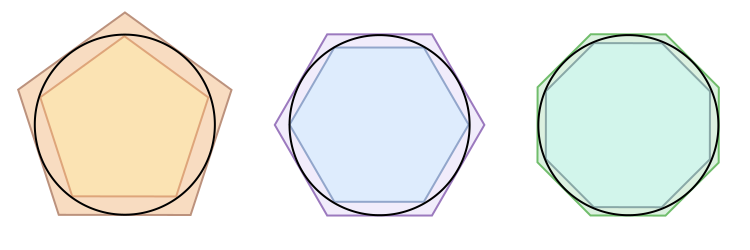
\includegraphics[scale=0.4]{images/archimedes}
		\caption{Aproximaciones de $\pi$ mediante polígonos regulares.}
		\label{fig:Arquimedes}
\end{figure}

Al calcular los perímetros de estos polígonos
Arquímedes logró demostrar que
\[
	3,1408=\frac{223}{71}<\pi<\frac{22}{7}=3,1429
\]

En otras civilizaciones encontramos distintas aproximaciones para el número
$\pi$. En la matemática china, por ejemplo, nos encontramos con que $\pi$ era
aproximado por $3,1547$ y también por $\sqrt{10}$. Cerca del año 265 el
matemático chino Liu Hui divisó un algoritmo que le permitió aproximar $\pi$
como $3,1416$.  En el año 480 el matemático chino Zu Chongzhi mostró que 
\[
	3,1415926<\pi<3,1415927
\]
y sugirió que $\pi$ fuera aproximado por los racionales $355/113$ y $22/7$. 

El cálculo del número $\pi$ es un tema que ocupa un lugar preponderante en la
historia de la matemática. Hay muchos matemáticos y muchas técnicas distintas
que quizá convendría exponer, pero tal tarea nos llevaría mucho tiempo y solo
podríamos hacerlo a expensas de sacrificar la presentación de otros resultados
también importantes en el desarrollo de la matemática. Para más información
sobre el cálculo de $\pi$ referimos al libro~\cite{MR0449960}. 

Creemos que el primer matemático que utilizo la letra griega $\pi$ para denotar
al cociente entre la circunferencia y el diámetro fue William Jones en 1706.
Euler utilizó la letra $\pi$ para denotar esta famosa constante en su libro de
1736 sobre mecánica. 

La aparición de las series infinitas en los siglos XVI y XVII permitieron
obtener mejores aproximaciones para $\pi$ que aquellas encontradas por
Arquímedes mediante métodos geométricos. 

\label{Vieta}
\label{Wallis}
En 1593 Vieta encontró la
expresión
\[
	\frac{2}{\pi}=\dfrac{\sqrt{2}}{2}\dfrac{\sqrt{2+\sqrt{2}}}{2}\dfrac{\sqrt{2+\sqrt{2+\sqrt{2}}}}{2}\cdots
\]
y en 1655 Wallis encontró una expresión que involucra productos infinitos:
\[
	\frac{\pi}{2}=\frac21\frac23\frac43\frac45\frac65\frac67\frac87\frac89\cdots
\]

\label{LeibnizGregory}
El cálculo de Leibniz y Newton permitió obtener muchas otras expresiones
infinitas que involucran al número $\pi$. Gregory y Leibniz, alrededor del año
1670, descubrieron, independientemente la expresión
\[
	\frac{\pi}{4}=1-\frac13+\frac15-\frac17+\cdots
\]
al especializar en un cierto valor la expansión en serie 
\[
	\arctan x=x-\frac{x^3}{3}+\frac{x^5}{5}-\cdots,
\]
encontrada por primera vez en la matemática india en el siglo XV.

En 1761 Lambert demostró que $\pi$ es irracional.  La demostración que dio
Lambert sobre la irracionalidad de $\pi$ es bastante difícil, se basa en la
siguiente expansión para la tangente:
\[
	\tan(x)=\dfrac{x}{1-\dfrac{x^2}{3-\dfrac{x^2}{5-\dfrac{x^2}{7-\cdots}}}}
\]

Hermite dio otra demostración de la irracionalidad de $\pi$ en 1873, y esta
demostración es mucho más sencilla que aquella encontrada por Lambert. 

En 1941 Niven encontró una demostración muy breve y sencilla, que bien podría
darse en cualquier curso de cálculo. Esta demostración utiliza ingeniosamente
algunas de las ideas de Hermite. Veamos la demostración de la irracionalidad de
$\pi$ encontrada por Niven:

\begin{theorem}
	\index{Irracionalidad!de $\pi$}
	El número $\pi$ es irracional.	
\end{theorem}

\begin{proof}
	Supongamos que $\pi=a/b$ con $a$ y $b$ enteros positivos. Sea 
	\[
		f(x)=\frac{x^n(a-bx)^n}{n!}.
	\]

	Primero observemos que $f$ es un polinomio de la forma
	$f(x)=\frac{1}{n!}\sum_{j=n}^{2n}c_jx^j$, donde los $c_j$ son números
	enteros. En efecto, por la fórmula del binomio, 
	\[
		f(x)=\frac{1}{n!}\sum_{j=0}^n\binom{n}{j}a^jx^{2n-j},
	\]
	que puede reescribirse como $f(x)=\sum_{j=n}^{2n}c_jx_j$ para ciertos
	enteros $c_j$.  En particular, $f^{(k)}(0)=\frac{k!}{n!}c_k\in\Z$ si $n\leq
	k\leq 2n$. Como además $f(x)=f(a-bx)$, se demuestra fácilmente por
	inducción que $f^{(k)}(x)=(-b)^kf^{(k)}(a-bx)$ para todo $k$. Luego
	$f^{(k)}(\pi)=(-b)^kf^{(k)}(0)$ para todo $k$. Esto implica que si definimos 
	\[
	F(x)=f(x)-f^{(2)}(x)+f^{(4)}(x)-\cdots+(-1)^nf^{(2n)}(x), 
	\]
	entonces $F(0)+F(\pi)\in\Z$. 

	Como $f(x)$ es un polinomio de grado $2n$, tenemos que $f^{(2n+2)}(x)=0$ y
	luego $F''(x)+F(x)=f(x)$.  Un cálculo directo muestra entonces que
	\[
		\frac{d}{dx}\left( F'(x)\sin x-F(x)\cos x\right)=(F''(x)+F(x))\sin x=f(x)\sin x.
	\]
	En consecuencia, 
	\[
		\int_0^\pi f(x)\sin xdx=F(0)+F(\pi)\in\Z.
	\]
	En el intervalo $(0,\pi)$, las funciones $f(x)$ y $\sin x$ son estrictamente positivas.
	Sabemos además que en este intervalo vale que $0\leq x(a-bx)=xa-bx^2\leq
	\pi a$. 
	Luego
	\[
		0<\int_0^\pi f(x)\sin xdx\leq \int_0^\pi \frac{(\pi a)^n}{n!}dx=\frac{(\pi a)^n}{n!}\pi.
	\]
	Pero $\displaystyle{\lim_{n\to\infty}\frac{\pi^{n+1}a^n}{n!}=0}$, una contradicción.
\end{proof}

%En 1760 Lambert y Riccati, en forma independiente, introdujeron las funciones
%hiperbólicas y estudió algunas de sus propiedades. 

Quizá sea este un buen momento para permitirnos ir hacia otro tópico importante
en la historia de la matemática. Antes de irnos, mencionaremos una fantástica
fórmula encontrada por Euler en 1734: 
\begin{equation}
	\label{eq:pi^2/6}
\sum_{n=1}^{\infty}\frac{1}{n^2}=\frac{\pi^2}{6}.
\end{equation}

No vamos a demostrar en detalle esta fórmula pero sí mencionaremos brevemente
cómo podríamos demostrarla utilizando simplemente técnicas de cálculo. La idea
es calcular una cierta integral de dos formas distintas e igualar estos
resultados. La integral a calcular es 
\[
		I=\int_0^1\int_0^1 \frac{1}{1-xy}dxdy.
	\]
Como dijimos, debemos calcular $I$ de dos formas distintas.  Un método para
calcular esta integral consiste en escribir el integrando como una serie y
realizar algunos cálculos sencillos: 
	\begin{align*}
		I&=\int_0^1\int_0^1 \sum_{n\geq0}(xy)^ndxdy\\
		&=\sum_{n\geq0}\int_0^1\int_0^1 (xy)^ndxdy\\
		&=\sum_{n\geq0}\int_0^1x^ndx\int_0^1y^ndy\\
		&=\sum_{n\geq0}\frac{1}{n+1}\frac{1}{n+1}\\
		&=\sum_{n\geq1}\frac{1}{n^2}.
	\end{align*}
Otra forma de calcular $I$ involucra realizar algún ingenioso cambio de
variables. En efecto, si calculamos $I$ con el cambio de variables
$u=\frac{x+y}{2}$ y $v=\frac{-x+y}{2}$, podremos demostrar la fórmula
encontrada por Euler. 
%	\begin{align*}
%		I&=4\int_0^{1/2}\left(\int_0^u\frac{dv}{1-u^2+v^2}\right)du+4\int_{1/2}^1\left(\int_0^{1-u}\frac{dv}{1-u^2+v^2}\right)du\\
%		&=\dots
%	\end{align*}

\begin{exercise}
	Demuestre la fórmula~\eqref{eq:pi^2/6}.
\end{exercise}

Veamos cómo fue que Euler encontró la fórmula~\eqref{eq:pi^2/6}. Una de las
fórmulas de Newton para polinomios nos permite escribir polinomios como
\[
	1-\alpha_1x+\alpha_2x^2+\cdots+(-1)^k\alpha_kx^k
	=\left(1-\frac{x}{a_1}\right)\left(1-\frac{x}{a_2}\right)\cdots\left(1-\frac{x}{a_k}\right),
\]
donde 
\begin{align*}
	\alpha_1&=\frac{1}{a_1}+\frac{1}{a_2}+\cdots\\
	\alpha_2&=\frac{1}{a_1a_2}+\frac{1}{a_1a_3}+\cdots
\end{align*}
y así sucesivamente. En particular, 
\begin{align*}
	&\frac{1}{a_1^2}+\frac{1}{a_2^2}+\cdots = \alpha_1^2-2\alpha_2,\\
	&\frac{1}{a_1^3}+\frac{1}{a_2^3}+\cdots = \alpha_1^3-3\alpha_1\alpha_2+3\alpha_3,\\
	&\frac{1}{a_1^4}+\frac{1}{a_2^4}+\cdots = \alpha_1^4-4\alpha^2_1\alpha_2+4\alpha_1\alpha_3-4\alpha_4,
\end{align*}
y así sucesivamente. 

La arriesgada idea de Euler es la de utilizar una extensión de esta última
fórmula pero para series de la forma
\[
	1-\alpha_1x+\alpha_2x^2+\cdots,
\]
De hecho, en el caso particular de la serie
\[
	1-\sin x=1-x+\frac{x^3}{3!}-\frac{x^5}{5!}+\frac{x^7}{7!}-\cdots
\]
tenemos que, como la función $x\mapsto 1-\sin x$ tiene ceros en 
\[
	\frac{\pi}{2},\frac{\pi}{2},-\frac{3\pi}{2},-\frac{3\pi}{2},\frac{5\pi}{2},-\frac{7\pi}{2},-\frac{7\pi}{2},\dots
\]
la fórmula para $\alpha_1$ que vimos antes implica que
\[
	\frac{4}{\pi}\left(1-\frac13+\frac15-\cdots\right)=1,
\]
de donde inmediatamente se obtiene la fórmula de Gregory--Leibniz.  

Si utilizamos la
fórmula para $\alpha_1^2-2\alpha_2$ obtenemos además 
\[
	\frac{8}{\pi^2}\left(1-\frac13+\frac15-\cdots\right)=1.
\]
Luego
\begin{align*}
	\sum_{n=1}^\infty\frac{1}{n^2} &= \sum_{n=1}^\infty\frac{1}{(2n)^2}+\sum_{n=0}^\infty\frac{1}{(2n+1)^2}=\frac14\sum_{n=1}^\infty\frac{1}{n^2}+\frac{\pi^2}{8},
\end{align*}
de donde se deduce inmediatamente la fórmula~\eqref{eq:pi^2/6}.
Esta fórmula nos permite entender por qué algunas civilizaciones aproximaban a
$\pi$ con el número $\sqrt{10}$. Primero, observemos que 
\[
	\sum_{n=1}^\infty\frac{1}{n^2}=1+\sum_{n=2}^\infty\frac{1}{n^2}<\sum_{n=2}^\infty\frac{4}{4n^2-1}.
\]
Para sumar esta última serie, observamos que
\[
	\frac{4}{4n^2-1}=\frac{4}{(2n-1)(2n+1)}=\frac{2}{2n-1}-\frac{2}{2n+1}=\frac{2}{2n-1}-\frac{2}{2(n+1)-1}.
\]
Luego 
\[
	\sum_{n=1}^\infty\frac{1}{n^2}<1+\left(\frac23-\frac25\right)+\left(\frac25-\frac27\right)+\left(\frac27-\frac29\right)+\cdots=1+\frac23=\frac53
\]
y entonces $\pi^2<6(5/3)=10$. El error es bastante pequeño pues 
\begin{align*}
	\frac53-\sum_{n=1}^\infty\frac{1}{n^2}
	&=\sum_{n=2}^\infty\left(\frac{4}{4n^2-1}-\frac{1}{n^2}\right)\\
	&=\sum_{n=2}^\infty\frac{1}{n^2(4n^2-1)}
	\leq\sum_{n=2}^\infty\frac{16}{60x^4}
	<\int_1^{\infty}\frac{16}{60}t^4dt=\frac{16}{180}.
\end{align*}

Tal como hizo Euler, pueden usarse fórmulas similares para encontrar otras series 
que involucren potencias de $\pi$ como por ejemplo
\[
	1+\frac{1}{2^4}+\frac{1}{3^4}+\cdots=\frac{\pi^4}{90}.
\]
Para más información sobre el magistral manejo que Euler tenía con las series
infinitas referimos al artículo~\cite{MR2338363}.


\subsection*{El teorema del binomio}
\index{Teorema!del binomio}

El teorema del binomio fue mencionado en la demostración de Niven de la
irracionalidad de $\pi$. El resultado afirma que para un entero positivo $n$ vale la siguiente fórmula
\[
	(x+y)^n=\sum_{k=0}^n\binom{n}{k}x^ky^{n-k},
\]
donde
\[
	\binom{n}{k}=\frac{n!}{k!(n-k)!}
\]
son los coeficientes binomiales. Una versión más general afirma si $|x|<|y|$ y además 
$r\in\C$, entonces vale la siguiente fórmula 
\[
	(x+y)^r=\sum_{k=0}^\infty\binom{r}{k}x^{k}y^{r-k},
\]
donde 
\[
	\binom{r}{k}=\frac{r(r-1)\cdots (r-k+1)}{k!},
\]
expresión que coincide con los coeficientes binomiales si $n$ es un entero
positivo. 

\begin{example}
	Una aplicación sencilla de la fórmula del binomio nos da la siguiente fórmula, válida 
	para todo $x$ tal que $|x|<1$:
	\begin{align*}
		(1+x)^{-1}&=1-x+x^2-x^3+x^4+\cdots
	\end{align*}
\end{example}

%\begin{exercise}
%	Demuestre que para $x$ tal que $|x|<1$ valen las siguientes fórmulas:
%	\begin{align*}
%		\sqrt{1+x}&=1+\frac12x-\frac18x^2+\frac{1}{16}x^3-\frac{5}{128}x^4+\cdots,\\
%		\frac{1}{\sqrt{1+x}}&=1-\frac12x+\frac38x^2-\frac{5}{16}x^3+\frac{35}{128}x^4-\cdots
%	\end{align*}
%\end{exercise}

La primera aparición escrita de algo similar al
teorema del binomio aparece en uno de los libros de Euclides, donde se
demuestra que vale la fórmula
\[
	(a+b)^2=a^2+b^2+2ab.
\]
Euclides también demuestra una identidad similar:
\[
	a^2+b^2=2ab+(a-b)^2.
\]

Según Coolidge~\cite{MR28222}, Euclides estaba en condiciones de obtener
fácilmente la fórmula para el cubo de un binomio pero en épocas de Euclides se
priorizaba la claridad y la precisión y no se intentaba obtener resultados en
la forma más general posible como pasa en la matemática de la actualidad.  Se
cree que en el siglo V el matemático indio Aryabhata conocía la fórmula para el
cubo de un binomio, y que esta fórmula tenía interés dado que era utilizada
para aproximar raíces cúbicas. No sabemos si la matemática india estaba
interesada en otras potencias de un binomio, pero posiblemente este problema no
resultara de interés ya que carecía de aplicaciones prácticas. Alrededor del
año 1300 varios matemáticos chinos mostraron interés en lo que hoy
--injustamente-- conocemos como el triángulo de Pascal, que no es otra cosa que
la representación de los coeficientes binomiales ordenados en forma de
triángulo: 

\begin{center}
\begin{tabular}{rccccccccc}
    &    &    &    &  1\\\noalign{\smallskip\smallskip}
    &    &    &  1 &    &  1\\\noalign{\smallskip\smallskip}
    &    &  1 &    &  2 &    &  1\\\noalign{\smallskip\smallskip}
    &  1 &    &  3 &    &  3 &    &  1\\\noalign{\smallskip\smallskip}
  1 &    &  4 &    &  6 &    &  4 &    &  1\\\noalign{\smallskip\smallskip}
\end{tabular}
\end{center}

Se sabe que esta configuración de números era ya bien conocida desde tiempo antes, en
particular en la matemática china y árabe. Varios historiadores creen que los
matemáticos chinos sabían además cómo calcular elevadas potencias de un binomio. 

En 1544 un monje alemán llamado Stifel publicó \emph{Arithmetica integra}, un
importante tratado sobre aritmética donde aparece una lista de números enteros
que hoy interpretamos como la fórmula
\[
	\binom{n}{k}=\binom{n-1}{k}+\binom{n-1}{k-1}.
\]

El tratado de Stifel contiene además importantes avances en 
notación matemática (escribir la multiplicación por juxtaposición, por ejemplo,
o el uso del término ``exponente'' para las potencias, así como también
la introducción del término ``coeficiente binomial''), contiene una tabla de
potencias de dos que no es sino una forma precaria de una tabla de logaritmos,
trata a los números negativos de la misma forma que trata a los números
positivos, sin ninguno de los prejuicios que los negativos enfrentaban en
aquellos tiempos. Stifel además estudió en su tratado propiedades de los
números irracionales y concluye que tales números son necesarios en la
matemática. 

En 1655 Pascal publicó un tratado donde figuran muchos resultados sobre los
coeficientes binomiales y  utilizó además estos resultados para resolver
problemas de la teoría de probabilidades. Fue en esta publicación donde Pascal
observó que la cantidad de subconjuntos de $k$ elementos de un conjunto de $n$
elementos es igual a 
\[
	\binom{n}{k}=\frac{n!}{k!(n-k)!},
\]
aunque aparentemente esta fórmula era ya conocida por Briggs en 1620.  En 1708
Pierre Rémond publicó un tratado sobre los juegos de azar y fue precisamente en
aquel libro donde le atribuyó a Pascal la invención del triángulo formado por
los coeficientes binomiales. 

Años más tarde, Gregory e independientemente Newton consideraron necesario
poder calcular potencias fraccionarias de binomios y obtuvieron algunos
resultados. Newton, por ejemplo, encontró la fórmula
\begin{align*}
	(1-x^2)^{1/2}&=1-\frac{x^2}{2}-\frac{x^4}{8}-\frac{x^6}{16}\cdots,
\end{align*}
aunque no sabemos exactamente cuál fue el método que le permitió obtener esa y
otras fórmulas similares. Coolidge afirma que no es justo decir que Newton
demostró el teorema del binomio, ya que, según parece, el gran genio inglés
simplemente mostró que en ciertos casos la fórmula sugerida por el teorema
del binomio daba el resultado correcto si el exponente era un cierto número
racional. 

Para encontrarnos con algunos de los primeros pasos hacia obtener una
demostración rigurosa del teorema del binomio debemos saltar hacia 1742, año en
un matemático italiano de apellido Salvemini publicó un trabajo donde menciona
que todos conocen al teorema de Newton pero nadie parece haberlo demostrado.
Demuestra entonces el teorema del binomio después de haber distinguido tres
posibles casos: a) el exponente es un entero positivo, b) el exponente es una
fracción positiva, y por último c) el exponente es negativo. Ese mismo año una
demostración mucho más breve e ingeniosa aparece en \emph{A treatise on
Fluxions}, un libro de 736 páginas escrito por el matemático escocés Colin
Maclaurin. La demostración de Maclaurin es más o menos así: Supongamos que
queremos calcular $(1+x)^n$, donde $n$ es un número racional positivo o
negativo. Escribimos entonces
\[
	(1+x)^n=1+Ax+Bx^2+Cx^3+\cdots
\]
Al derivar ambos miembros de la igualdad obtenemos la identidad
\begin{equation}
	\label{eq:Maclaurin}
	n(1+x)^{n-1}=A+2Bx+3Cx^2+\cdots
\end{equation}

Al reemplazar $x$ por cero en esta igualdad, obtenemos que $A=n$. Si derivamos
la igualdad~\eqref{eq:Maclaurin} para luego evaluar la nueva identidad en
$x=0$, podremos calcular explícitamente el valor de $B$. El resto de los
coeficientes se obtendrá entonces muy fácilmente mediante esta técnica que
involucra el cálculo de derivadas. Seguramente muchos lectores estarán algo incómodos, ya que 
en esta ``demostración'' hay varias cosas
que falta justificar, de eso no hay duda. Un agujero particularmente importante
es el de la convergencia. ¡Debemos asegurarnos de que las series convergen!
Este problema era reconocido por Maclaurin, pero no fue capaz de resolverlo. El
primer matemático capaz de resolver los problemas de convergencia 
en relación al teorema del binomio fue Abel y lo hizo en
1826. 


% numeros de bernoulli


\chapter{La geometría griega}

En este capítulo hablaremos de la geometría griega. Naturalmente una parte
sustancial de este capítulo estará dedicada a los famosos trece libros de
Euclides. Si bien cada vez que sea necesario transcribir partes de los libros
de Euclides utilizaremos una traducción al castellano hecha por María Luisa
Puertas Castaño~\cite{elementos1,elementos2}, quizá sea oportuno remarcar que el interesado en un estudio
histórico más profundo de la matemática contenida en estos libros de Euclides
deberá consultar la excelente versión de los libros de Euclides traducida y
comentada por el historiador de la matemática (y además experto en la
matemática griega) Thomas Heath~\cite{MR1932864}. 

Para los griegos, la geometría era la rama más importante de la matemática.
Alrededor del 300 a. C. Euclides organizó gran parte de la matemática que se
conocía en aquel momento y escribió trece libros.  El tratado de Euclides fue
el texto más influyente en la historia de la matemática y fue fundamental quizá
hasta principios del siglo XX. 

Es poco lo que se conoce de la matemática anterior a la época de Euclides. En
sus comentarios sobre los elementos de Euclides, Proclo hace un breve resumen
histórico; muy posiblemente este resumen esté fuertemente basado en un tratado
sobre historia de la matemática escrito por Eudemo. Proclo menciona que muchos
autores atribuyen a los egipcios la invención de la geometría, nacida para
atacar problemas prácticos tales como la medición de campos. Proclo además
afirma que los fenicios fueron los primeros en tener un conocimientos de los
números debido a las transacciones comerciales. Según Proclo, Tales estuvo en
egipto y fue el primero en llevar la geometría a Grecia. El estudio sistemático
de la geometría, con teoremas abstractos que se obtienen a partir de principios
generales, se le atribuye a los miembros de la escuela de Pitágoras. Platón
mostró gran interés en la geometría y justamente eso fue lo que le dio un
impulso extraordinario.

%A Tales se le atribuyen varias constribuciones geométricas fundamentales, por ejemplo que todo diámetro biseca a la circunferencia, 
%que los ángulos de la base de un triángulo isósceles son iguales, que ángulos opuestos por el vértice son iguales, y la resolución
%de varios problemas de aplicación como el de calcular la distancia entre una nave y el puerto, o calcular
%la altura de una pirámide sabiendo cuánto mide la sombra que proyecta. 
%El resultado que hoy conocemos como el teorema de Tales aparece en el libro VI de los elementos. 

Los libros de Euclides comienzan con definiciones (que para nosotros quizá no
siempre resultan del todo precisas). Por ejemplo, el \emph{punto} se define
como lo que no tiene partes; esta es la primera definición. La segunda
definición dice que una \emph{línea} es una longitud sin anchura. La tercera,
que los extremos de una línea son puntos. (Hay que aclarar que estas
definiciones fueron tomadas de la traducción de los elementos hecha por Puertas
Castaño.) Figuran en los libros de Euclides 
además las definiciones de círculo, ángulos rectos y agudos,
etc.

Después de las definiciones, se presentan los postulados. El primero de los
postulados afirma que siempre existe una línea recta que une dos puntos
distintos del plano. En mi traducción\footnote{La versión de los Elementos que
	se utilizará en este curso, y en particular durante este capítulo, es una
	edición la editorial Gredos, con traducción y notas de María
Luisa Puertas Castaños.}, leo la siguiente oración: 
\begin{quote}
	Postúlese el trazar una línea recta dado un punto cualquiera hasta un punto
	cualquiera. 
\end{quote}
El segundo postulado afirma que es posible prolongar continuamente una recta
finita en línea recta; es decir: se afirma que una línea puede extenderse tanto
como sea necesario en cualquiera de las dos direcciones posibles.  El tercer
postulado afirma que dado un punto $P$ y una distancia $r$, puede construirse
un círculo con centro en $P$ y radio $r$. Uno de estos postulados, el quinto,
es particularmente importante dentro del desarrollo histórico de la matemática: 

\begin{quote}
	Si una recta al incidir sobre dos rectas hace los ángulos internos del
	mismo lado menores que dos rectos, las dos rectas prolongadas
	indefinidamente se encontrarán en el lado en el que estén los (ángulos)
	menores que dos rectos.
\end{quote}

En este postulado se basa un hecho notable: la geometría de los libros de
Euclides no es sino una de las geometrías posibles. Es sorprendente que
Euclides haya considerado necesario incluir este quinto postulado para fijar
condiciones que garanticen que dos rectas se corten en un único punto.  Más de
dos mil años después de aquella genialidad, al reemplazar este postulado la
matemática encontrará geometrías distintas a la geometría estudiada por
Euclides, las denominadas geometrías no euclidianas.

Además de los postulados hay doce \emph{nociones comunes}. La primera de estas
nociones comunes afirma que \emph{las cosas iguales a una misma cosa son
también iguales entre sí}. En nuestro lenguaje algebraico, esto equivale a que
si $A=B$ y además $A=C$, entonces $B=C$.  

A partir de esas definiciones básicas, de los axiomas y los postulados,
Euclides desarrolló la geometría. Por ejemplo, la primera proposición del libro
I explica cómo construir un triángulo equilátero sobre una recta finita dada.
La proposición es acompañada por una figura similar a la
figura~\ref{fig:libroI_prop1}. 

\begin{figure}
   \centering
   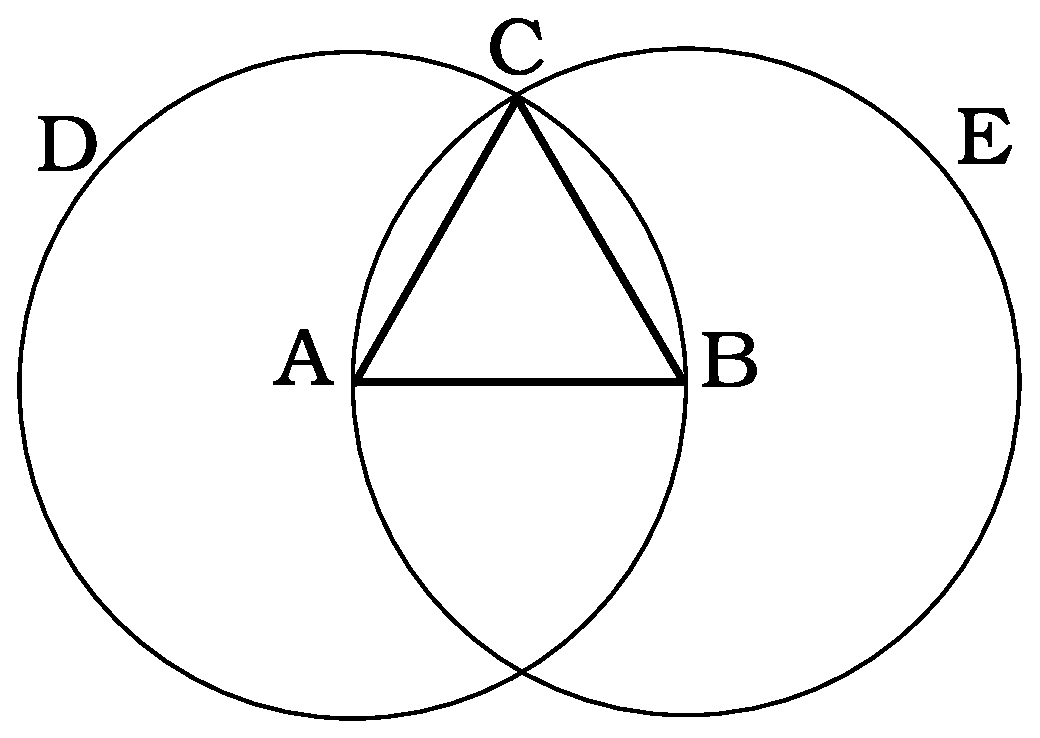
\includegraphics[scale=0.2]{images/libroI_prop1}
   \caption{La proposición 1 del libro I.}
   \label{fig:libroI_prop1}
\end{figure}

La demostración es breve y sencilla, aunque no es del todo convincente pues
faltan justificaciones. Es la primera demostración de los libros de Euclides, y
quizá por eso acumula muchas más críticas que las otras demostraciones.  

La proposición 47 del libro I es el teorema de Pitágoras: 
\begin{quote}
	En los triángulos rectángulos el cuadrado del lado que subtiende el ángulo
	recto es igual a los cuadrados de los lados que comprenden el ángulo recto.
\end{quote}
Se cree que la demostración basada en la figura~\ref{fig:libroI_prop47} fue
descubierta por Euclides.


\begin{figure}
   \centering
   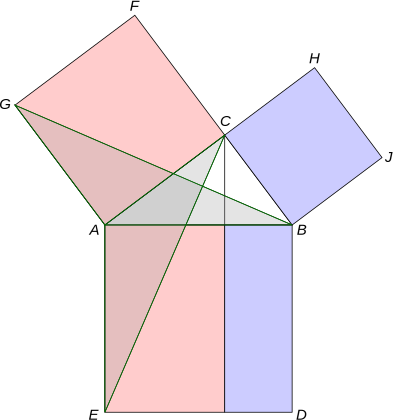
\includegraphics[scale=0.4]{images/libroI_prop47}
   \caption{La demostración del teorema de Pitágoras dada por Euclides.}
   \label{fig:libroI_prop47}
\end{figure}

En el segundo libro aparecen ciertas nociones algebraicas, aunque en un
lenguaje completamente distinto al que usamos en estos tiempos. La primera
proposición de este libro, por ejemplo, afirma lo siguiente: 
\begin{quote}
	Si hay dos rectas
	y una de ellas se corta en un número cualquiera de segmentos, el rectángulo
	comprendido por las dos rectas es igual a los rectángulos comprendidos por la
	(recta) no cortada y cada uno de los segmentos.
\end{quote}
Nuestra notación algebraica
nos permite reconocer en esta proposición la propiedad distributiva: 
\[
	a(b+c+\cdots)=ab+ac+\cdots
\]
La cuarta proposición afirma lo siguiente: 

\begin{quote}
	Si se corta al azar una línea recta,
	el cuadrado de la (recta) entera es igual a los cuadrados de los segmentos y
	dos veces el rectángulo comprendido por los segmentos.
\end{quote}
Esta proposición puede traducirse de la siguiente forma:
\[
	(a+b)^2=a^2+2ab+b^2.
\]

Las proposiciones 12 y 13 del libro II contienen resultados similares al
teorema del coseno, aunque sin hacer uso de funciones trigonométricas. La
trigonometría se desarrolló algún tiempo después de que Euclides escribió sus
Elementos. 

%Veamos otro resultado, ahora del tercer libro.  La proposición 35 del libro III
%afirma lo siguiente: 
%
%\begin{quote}
%Si en un círculo se cortan dos rectas entre sí, el
%rectángulo comprendido por los segmentos de una es igual al rectángulo
%comprendido por los segmentos de la otra.
%\end{quote}
%
%En lenguaje moderno esta proposición puede enunciarse de la siguiente forma: 

Recordemos que los griegos no podían medir distancias pero sí sabían cómo
comparar segmentos y reconocer cuándo dos segmentos son iguales o cuándo uno
es, digamos, el doble de otro. Los griegos tampoco podían medir ángulos. Gran
parte de la manera de pensar de los griegos era geométrica. Para ellos lo que
ahora sería el producto $ab$ entre los números $a$ y $b$ era simplemente el
área de un rectángulo de lados $a$ y $b$. La ecuación $ab=cd$ era interpretada
entonces como la igualdad entre las áreas de ciertos rectángulos.

En los libros de euclides hay además construcciones explícitas con regla y
compás, aunque Euclides en ningún momento hace referencia a estos u otros
instrumentos geométricos. 

\begin{exercise}
	Construya con regla y compás el punto medio de un segmento.
\end{exercise}

El mismo truco permite también construir un triángulo equilátero si uno de los
lados está dado.

\begin{exercise}
	Construya con regla y compás un cuadrado.	
\end{exercise}

Una pregunta interesante es la siguiente: ¿cómo puede construirse con regla y
compás un pentágono regular? Euclides dio una construcción.

\begin{exercise}
	Construya un pentágono regular con regla y compás. 
\end{exercise}

Es natural preguntarse cómo puede construirse o hexágono regular o, más
generalmente, cualquier $n$-ágono regular. Construir un hexágono es fácil ya
que sabemos construir triángulos equiláteros. Sin embargo, no puede construirse
un heptágono regular con regla y compás. Sí podemos, en cambio, construir un
octágono. 

En 1796 Gauss pudo construir con regla y compás un polígono regular de $17$
lados. Gauss no solamente encontró la forma de construir ese polígono regular
sino que demostró además que un polígono regular de $n$ lados puede construirse
con regla y compás sí y sólo si $n=2^mp_1\cdots p_k$ con $p_1,\dots,p_k$ primos
de Fermat distintos. Los primos de la forma 
\[
	p=2^{2^l}+1
\]
se conocen como \textbf{primos de Fermat}. Hasta el momento los únicos primos
de Fermat conocidos son los siguientes:
\[
	3,5,17,257,65537.
\]
Y se conjetura que esos son los únicos primos de Fermat que existen. Para más
información acerca de los primos de Fermat referimos a
las sucesiones 
\href{https://oeis.org/A000215}{A000215}.
y \href{https://oeis.org/A019434}{A019434}.

\index{Problema!de la trisección del ángulo}
\index{Problema!de la cuadratura del círculo}
\index{Problema!de la duplicación del cubo}
Las construcciones con regla y compás ocupaban un lugar importante en el
pensamiento de los geómetras griegos. Los griegos sabían cómo construir
$\sqrt{2}$ e incluso cómo construir $\sqrt{n}$ para cualquier $n$. Sin embargo,
no sabían cómo construir $\sqrt[3]{2}$; este problema se conoce como el
\textbf{problema de la duplicación del cubo}, ya que el problema consiste en
duplicar el volumen de un cubo dado). Otros problemas similares que mucho
interesaban a los griegos son los siguientes: el
\textbf{problema de la trisección de un ángulo} y el \textbf{problema de la
cuadratura del círculo} (en este problema se pide construir un cuadrado de área
igual al área de un círculo dado, o bien, equivalentemente, construir $\pi$).

Los pitagóricos habían resuelto el problema de la cuadratura de los polígonos.
Antifón demostró que dado un polígono inscrito en un círculo, siempre se puede
duplicar la cantidad de lados del polígono. De esto, concluyó erroneamente que
el círculo es cuadrable ya que puede aproximarse con arbitraria precisión por
polígonos cuadrables. Aristóteles observó que estos polígonos jamás llenarán al
círculo, sin importar qué tan grande sea el número de lados empleado. Tiempo
más tarde, Brisón mejoró el argumento y consideró sucesiones de polígonos
inscritos y circunscritos que aproximan cada vez mejor al círculo. Esta idea
fue retomada muy exitosamente por Arquímedes en sus trabajos sobre
aproximaciones del número $\pi$. Hipócrates redujo el problema de la cuadratura
del círculo a un problema de geometría plana. Si bien no logró resolver
complemente el problema de la cuadratura del círculo, sí logró cuadrar ciertos
recintos limitados por arcos, algo que hoy conocemos como \emph{lúnulas de
Hipócrates}

\begin{figure}
   \centering
   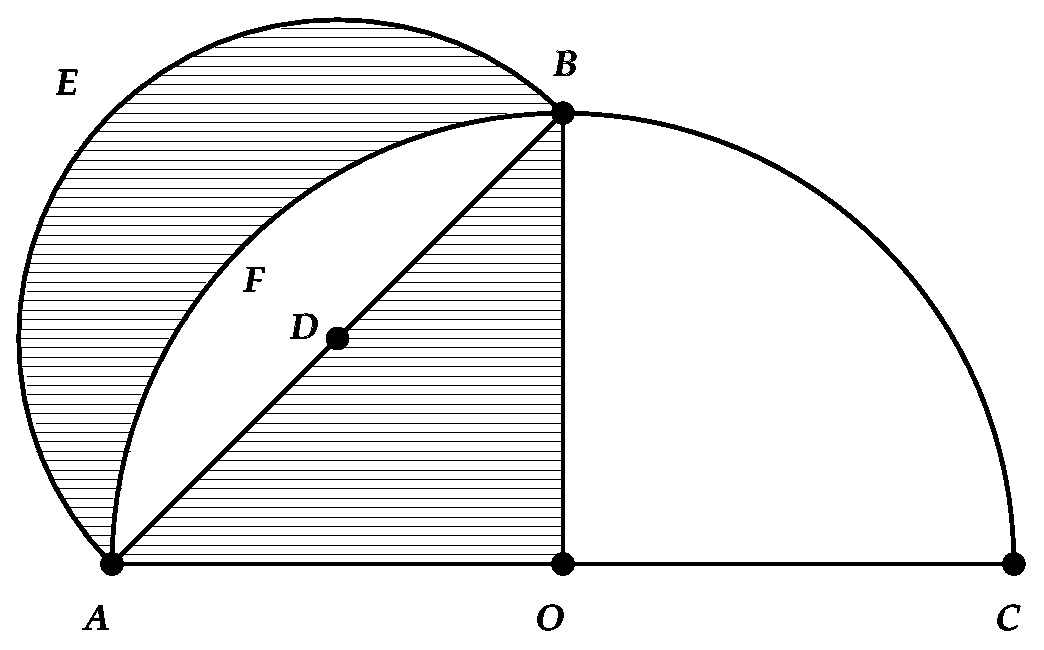
\includegraphics[scale=0.3]{images/lunula}
   \caption{Las lúnulas de Hipócrates.}
   \label{fig:lunula}
\end{figure}

\index{Lúnulas de Hipócrates}
Hipócrates probó que las áreas
sombreadas que vemos en la figura~\ref{fig:lunula} coinciden. La demostración del
resultado sobre lúnulas de Hipócrates es más o menos así: Sabemos que $D$ es el
centro del círculo que incluye el arco $AEB$, y es también el punto medio entre $A$
y $B$, que es la hipotenusa del triángulo $ABO$. Como $ABO$ es rectángulo e
isósceles, el diámetro $AC$ del círculo grande es $\sqrt{2}$ veces el tamaño del
diámetro del círculo que incluye al arco $AEB$. Como el área del círculo que
incluye al arco $ABC$ es la mitad del área del círculo que incluye al arco $AEB$,
entonces el área del cuarto de círculo $AFBOA$ es igual al área del semicírculo
$AEBDA$. Esto implica que las áreas sombreadas coinciden ya que ambas se obtienen
al restar el $AFBDA$ de regiones con la misma área. 

%Lamentablemente, el libro de Hipócrates se perdió, pero muy posiblemente haya
%servido de modelo para los Elementos de Euclides.

\begin{exercise}
	¿En qué consiste el problema de la trisección de un ángulo?
\end{exercise}

\index{Cuadratiz de Hipias}
Hipias logró resolver el problema de la trisección de un ángulo si se admite el
uso de una curva especial, que, tal como se demostró muchos años después, 
también permite
resolver el problema de la cuadtratura del círculo. Esta curva hoy se conoce
como la \emph{cuadratiz de Hipias} y puede describirse por la siguiente
función
\[
x\mapsto x\cot\left(\frac{\pi}{2a}x\right).
\]
Una representación gráfica en el caso $a=1$ puede verse en 
la figura \ref{fig:cuadratiz}.

\begin{figure}
   \centering
   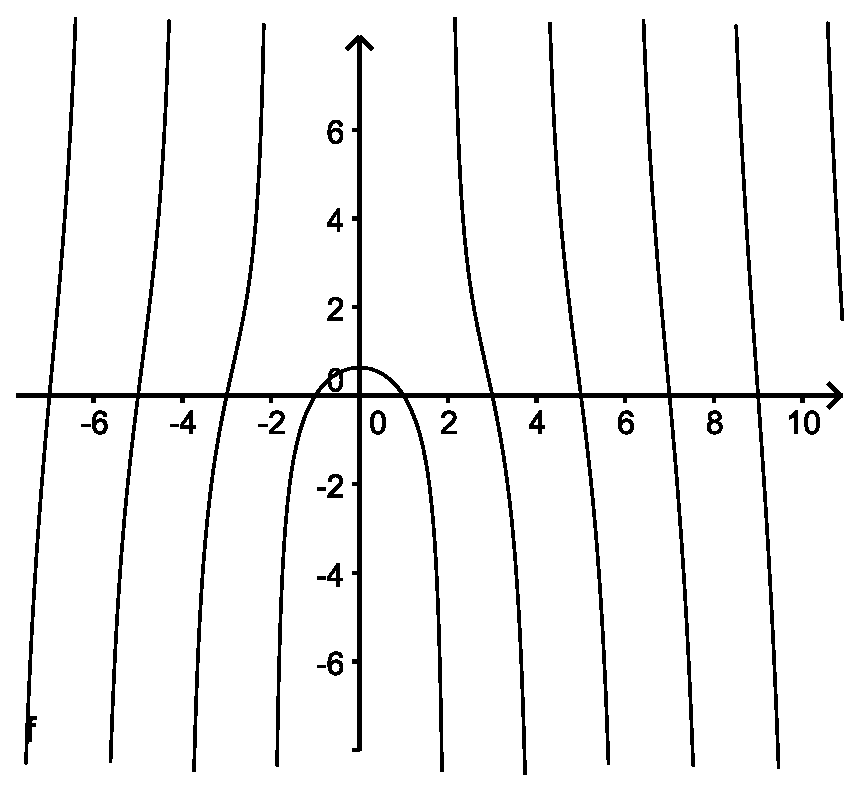
\includegraphics[scale=0.3]{images/cuadratiz}
   \caption{La cuadratiz de Hipias.}
   \label{fig:cuadratiz}
\end{figure}


% Agregar las ecuaciones y el svg de la página de wikipedia

\begin{exercise}
	¿Cómo puede construirse el número $\sqrt{n}$ con regla y compás?
\end{exercise}

\index{Número!trascendente}
\index{Número!algebraico}
\index{Número!construible}
Hoy sabemos que ninguno de estos tres problemas clásicos de la matemática
griega tiene solución. 

El problema de la duplicación del cubo y de la
trisección de un ángulo fue resuelto en 1837 por un matemático francés llamado
Pierre Wantzel. Poca gente hoy sabe que Wantzel fue el primer matemático que
fue capaz de resolver esos famosos problemas, quizá porque los métodos de
Wantzel fueron opacados por las ideas provenientes de la teoría de Galois.  

El
problema de la cuadratura del círculo fue resuelto por Lindelmann en 1882 al
demostrar que el número $\pi$ es trascendente. Un número se dice
\textbf{trascentente} si no es un número algebraico, es decir si no es raíz de
un polinomio con coeficientes racionales. Los números trascendentes, en
particular, no pueden construirse con regla y compás:
\[
	\{\text{números construibles}\}\subsetneq\{\text{números algebraicos}\}
\]

\index{Sólidos platónicos}
\index{Poliedro regular}
Otro gran descubrimiento importante para griegos es la construcción de los cinco
sólidos platónicos existentes. Un sólido platónico es un poliedro regular
convexo acotado por un cierto número de caras. Los sólidos platónicos son los
análogos espaciales de los polígonos regulares del plano. Sorprendentemente, y
a diferencia de lo que pasa con los polígonos regulares en el plano, existen
únicamente cinco poliedros regulares: el tetraedro, el cubo, el octaedro, el
dodecaedro y el icosaedro. No es difícil demostrar que, de existir poliedros
regulares, hay únicamente cinco posibilidades (y se cree que este resultado era
ya conocido por los pitagóricos). La dificultad está en demostrar que
efectivamente existen esos cinco poliedros; la dificultad está en poder
construir explícitamente esos cinco poliedros. Es fácil construir el tetraedro
o el cubo pero ¿cómo podemos construir, por ejemplo un icosaedro? Euclides no
solamente reconoció la dificultad y la belleza de este problema, sino que lo
resolvió y lo ubicó cerca del final de sus elementos. 

\begin{figure}
   \centering
   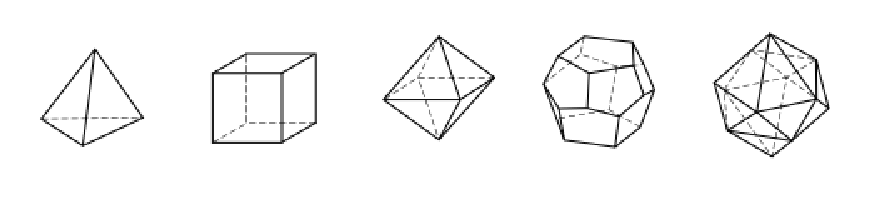
\includegraphics[scale=0.7]{images/platonic}
   \caption{Los sólidos platónicos.}
   \label{fig:platonic}
\end{figure}

Hay cierta controversia alrededor de los verdaderos descubridores de los
sólidos platónicos. La tradición nos dice los orígenes del dodecaedro, del cubo
y del octaedro están en los pitagóricos. Se nos dice además que el octaedro y
el icosaedro fueron descubiertos por Teeteto, colaborador de Platón. 

Hay gente que cree que los sólidos platónicos son muy anteriores,
creencia que se basa en la existencia de ciertas piedras del período neolítico
encontradas en Escocia, y que podemos ver en la figura~\ref{fig:piedras}. En la
opinión de Lloyd~\cite{MR2992714}, a pesar de que haber encontrado estas piedras resulte
un hecho absolutamente fascinante, 
existe poca o nula evidencia de que las piedras neolíticas de la
figura~\ref{fig:piedras} tengan alguna relación con la matemática. 
 
\begin{figure}
   \centering
   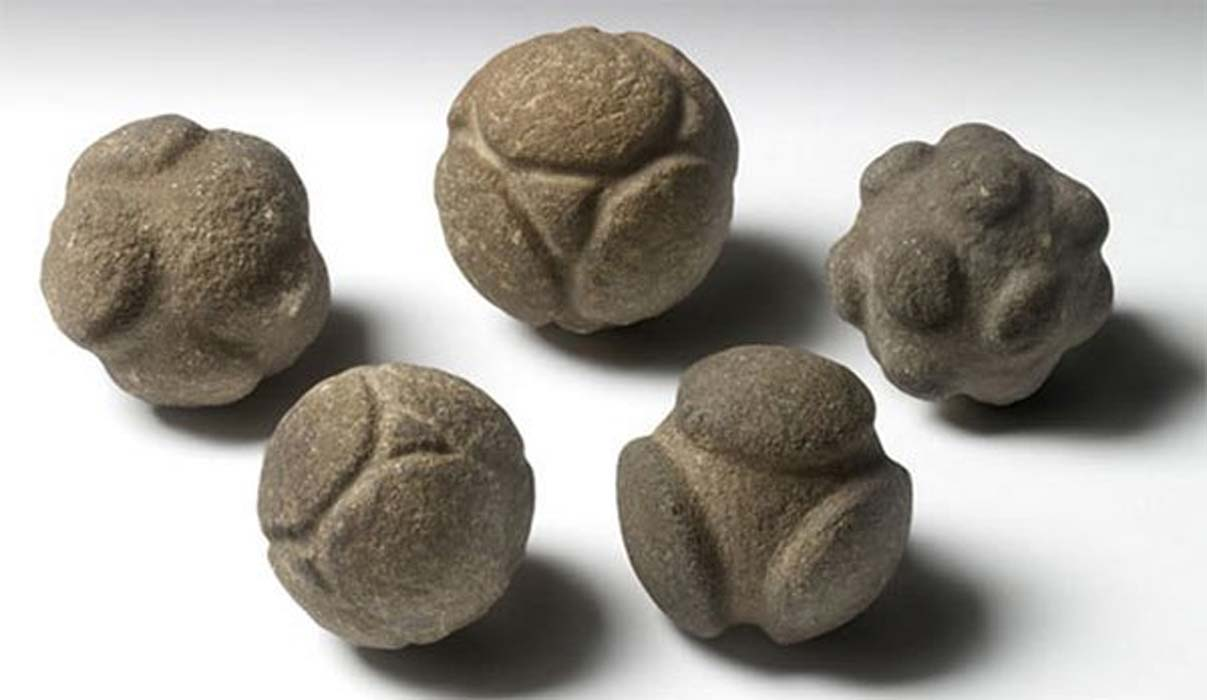
\includegraphics[scale=0.1]{images/stones}
   \caption{Piedras del período neolítico encontradas en Escocia.}
   \label{fig:piedras}
\end{figure}



En 1596 Kepler presentó una teoría sobre las distancias planetarias donde los
cinco poliedros regulares ocupan un rol fundamental. La teoría
de Kepler describe las órbitas planetarias como esferas encajadas
entre sólidos platónicos. 

\begin{figure}
   \centering
   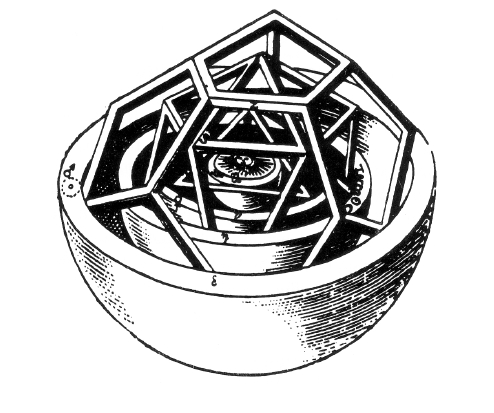
\includegraphics[scale=0.3]{images/kepler}
   \caption{La teoría de Kepler sobre órbitas planetarias.}
   \label{fig:kepler}
\end{figure}

Kepler observó que la existencia de únicamente cinco poliedros regulares era
compatible con la existencia de únicamente seis planetas. El descubrimiento de
Urano en 1781 destrozó a la teoría de Kepler. De todas formas, no fueron
necesarios otros planetas para que la teoría de Kepler perdiera valor. 

En 1609
Kepler descubrió que las órbitas planetarias son elipses; este hecho fue
explicado en 1687 por la teoría gravitatoria de Newton. 



\begin{exercise}
	En 1509 Luca Pacioli presentó una ingeniosa construcción del icosaedro
	basada en la figura~\ref{fig:Pacioli}.  ¿Cuál es esa construcción?
\end{exercise}

\begin{figure}
   \centering
   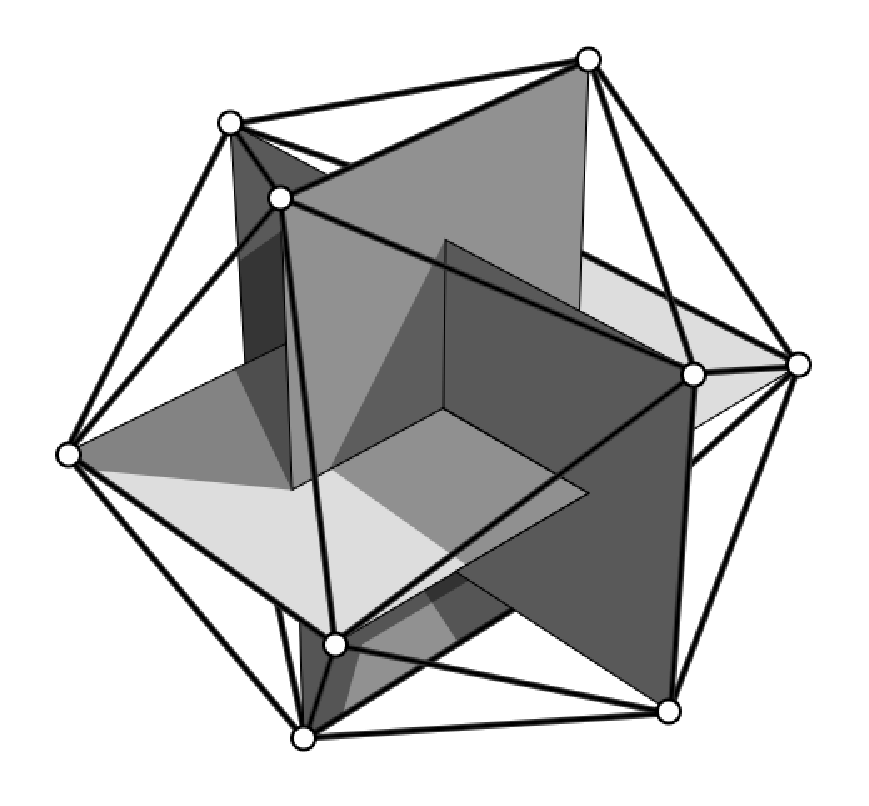
\includegraphics[scale=0.3]{images/pacioli}
   \caption{La construcción del icosaedro de Pacioli.}
   \label{fig:Pacioli}
\end{figure}

\index{Rectángulo áureo}
\index{Número!áureo}
La construcción del icosaedro dada por Pacioli utiliza rectángulos áureos. Un
rectángulo áureo es un rectángulo como el que vemos en la
figura~\ref{fig:golden} donde 
\[
	\frac{a+b}{a}=\frac{a}{b}.
\]

\begin{figure}
   \centering
   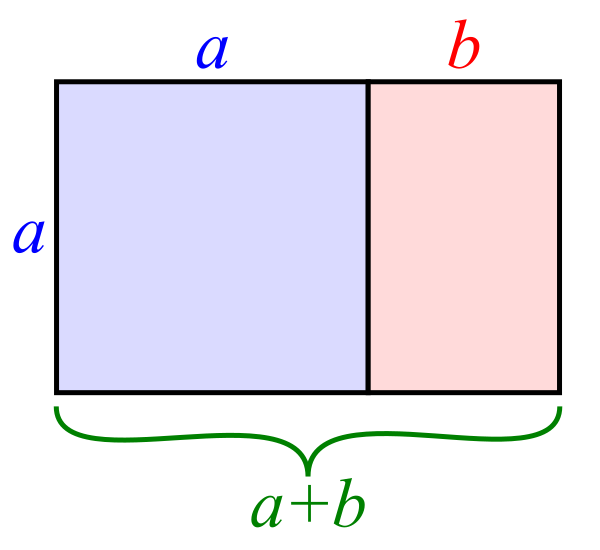
\includegraphics[scale=0.2]{images/golden}
   \caption{El rectángulo áureo.}
   \label{fig:golden}
\end{figure}

Puede demostrarse que el cociente $a/b$ es entonces solución de la ecuación
cuadrática $x^2-x-1=0$ y luego 
\[
	a/b=\frac{1+\sqrt{5}}{2}=1,6180339887\cdots,
\]
número que comunmente se denota con la letra griega $\varphi$.  La
figura~\ref{fig:construction} nos muestra que el número $\varphi$ es
construible con regla y compás. 

\begin{figure}
   \centering
   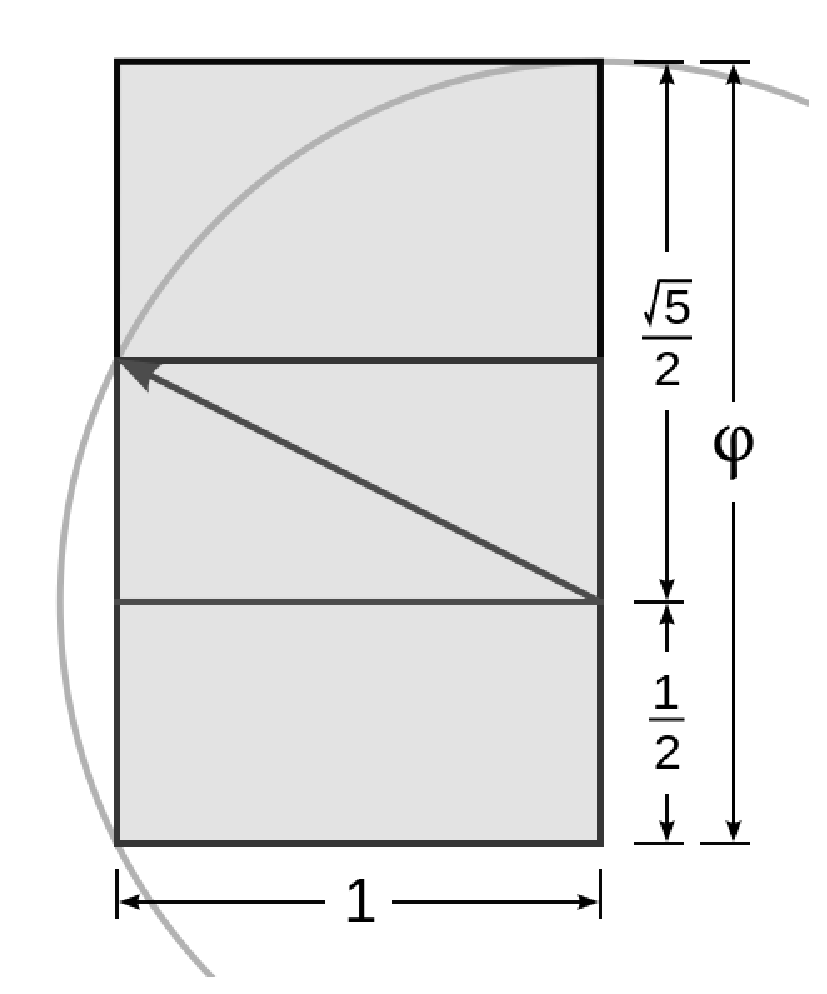
\includegraphics[scale=0.25]{images/construction}
   \caption{Una construcción con regla y compás del recángulo áureo.}
   \label{fig:construction}
\end{figure}

Hay varias expresiones curiosas del número $\varphi$. Puede expresarse por ejemplo como
la fracción continua 
\[
	\varphi=1+\cfrac{1}{1+\cfrac{1}{1+\cfrac{1}{1+\cdots}}}.
\]
También como el número trigonométrico 
$\varphi=2\cos(\pi/5)$ o 
como el límite
\[
	\varphi=\lim_{n\to\infty}\frac{F_n}{F_{n-1}},
\]
donde $F_n$ es el $n$-ésimo término de la sucesión 
\href{https://oeis.org/A000045}{A000045}.
de Fibonacci. 
Otra curiosa expresión para el número $\varphi$ es 
\[
	\varphi=\sqrt{1+\sqrt{1+\sqrt{1+\cdots}}}.
\]


\begin{exercise}
	Demuestre la veracidad de las expresiones del número $\varphi$ mencionadas
	en esta sección. 
\end{exercise}

Los rectángulos áureos aparecen en una tabla babilónica aproximadamente del año
850 a.C. que fue encontrada en Iraq en 1881. 

La publicación
en 1509 del libro \emph{Divina proportione} de Pacioli dio 
importancia al número $\varphi$,
especialmente entre artistas y arquitectos ya que los
rectángulos áureos son estéticamente más agradables que otros rectángulos. Hoy
en día es bastante fácil encontrarse con rectángulos áureos entre los objetos
que utilizamos comunmente. 

\section*{El método axiomático}

La intención original de Euclides fue la de deducir resultados a partir de
ciertas afirmaciones evidentes que llamó postulados (para nosotros, axiomas)
gracias al uso de ciertos principios básicos de la lógica. Estos libros de
Euclides constituyen el primer intento de derivar teoremas a partir de axiomas.
Según Heath, el método deductivo se le debe a Tales. 

Hoy en día nuestra forma de ver el método deductivo es levemente distinta.  El
método deductivo está basado en las leyes de la lógica y se compone de las
siguientes partes:
\begin{enumerate} 
	\item \emph{Términos primitivos}, que son ciertos elementos que no necesitan
			definirse tales como los puntos, las líneas y los planos de la
			geometría y las relaciones de incidencia entre ellos. No es
			importante el nombre que elijamos para estos elementos que no vamos
			a definir. 
		\item \emph{Axiomas o postulados}, que son ciertas afirmaciones acerca
			de los elementos primitivos, como bien podría ser el axioma que
			dice que dados dos puntos distintos existe una única línea recta
			que los contiene. Los axiomas se asumen verdaderos y no necesitan
			ser demostrados. 
		\item \emph{Teoremas}, que son simplemente las consecuencias lógicas de
			los axiomas.
\end{enumerate}

El rigor matemático de nuestro tiempo parece sugerir que el tratamiento
axiomático de Euclides no fue lo suficientemente riguroso. Sin embargo, no
tiene sentido mirar el texto de Euclides con nuestros ojos, hay que mirar la
matemática en perspectiva. En tiempos de Euclides el rigor matemático era
obviamente visto de forma completamente distinta. ¡Si la humanidad utilizó
durante dos mil años los libros de Euclides como libros de texto, seguro que no
fue por error o accidente! No parece apropiado criticar el rigor matemático
utilizado en los libros de Euclides después de recordar que fueron necesarios
dos mil años para entender cuáles eran los puntos de debilidad del tratado de
Euclides.

Veamos cuáles son los puntos donde hoy en día se critica el rigor matemático
del método axiomático de Euclides.  En los elementos de Euclides no existen los
términos primitivos, la lista de axiomas no es exhaustiva, algunas
demostraciones no están axiomáticamente justificadas, falta el uso de un cierto
principio de continuidad que garantice la existencia de ciertos puntos o líneas
que Euclides afirma que existen\dots Sí, nuestro rigor matemático se sentirá
levemente molesto por algunas cosas que encontramos en los libros de Euclides,
pero entre estas cosas hay una que se destaca notablemente. Una de las
diferencias fundamentales entre nuestra forma de ver el método axiomático y
aquella de Euclides está en el carácter que tienen los axiomas. ¡Los axiomas
elegidos no tienen por qué ser evidentes!  Hoy sabemos que hay otras geometrías
además de aquella de Euclides, y precisamente la existencia de estas otras
posibles geometrías no muestra que los axiomas elegidos pueden no ser
evidentes. ¿Acaso son evidentes las geometrías no euclidianas?

Si bien desde nuestro punto de vista moderno los axiomas impuestos por Euclides
tienen ciertas fallas, la matemática necesitó casi dos mil años para poder
encontrar fundamentos más precisos para la geometría. 

En el invierno de 1898
Hilbert dictó un curso en Gotinga sobre los fundamentos de la geometría. A
pedido de Klein, preparó notas poco tiempo después; notas que luego se
transformaron en un libro muy influyente, \emph{Grundlagen der Geometrie},
publicado en 1899, y que bien puede entenderse como una rectificación de la
geometría euclidiana. 

\section*{La fórmula de Herón}

\index{Fórmula!de Herón}
La fórmula de Herón nos dice que el área de un triángulo de lados $a$, $b$ y
$c$ está dada por la fórmula
\[
	\sqrt{s(s-a)(s-b)(s-c)},
\]
donde $s=\frac12(a+b+c)$. Esta fórmula puede demostrarse de muchas formas
distintas, por ejemplo con el teorema de Pitágoras o con la fórmula del coseno.

\begin{exercise}
	Utilice el teorema del coseno y demuestre la fórmula de Herón.
\end{exercise}

La fórmula aparece en el libro de Herón \emph{Métrica}, obra en tres volúmenes
donde Herón estudia las áreas de las superficies y los volúmenes de los
cuerpos. Estos libros estuvieron perdidos durante mucho tiempo,
hasta que fueron encontrados en 1896 por Schone en la ciudad de Constantinopla.
Una fórmula equivalente a la fórmula de Herón,
\[
	\frac14\sqrt{a^2b^2-\left(\frac{a^2+b^2-c^2}{2}\right)^2},
\]
fue encontrada en la matemática china y aparece en un libro publicado en 1247.

\index{Fórmula!de Arquímedes}
Se cree que Arquímedes conocía la fórmula de Herón pues entre sus escritos
figura el siguiente resultado: Supongamos que se tiene un triángulo $\Delta$ de
lados $q_1$, $q_2$ y $q_3$ y sean $Q_1=q_1^2$, $Q_2=q_2^2$ y $Q_3=q_3^2$.
Entonces 
\[
	16\times \textrm{área}(\Delta)^2=(Q_1+Q_2+Q_3)^2-2\times(Q_1^2+Q_2^2+Q_3^2).
\]

\begin{example}
	Consideremos en el plano el triángulo $\Delta$ con vértices en los puntos
	$(1,2)$, $(3,1)$ y $(0,0)$. Entonces
	\[
		16\times\textrm{área}(\Delta)=20^2-2\times(25+25+100)=400-2\times 150=100.
	\]
\end{example}

\index{Fórmula!de Brahmagupta}
La fórmula de Herón puede deducirse de una fórmula más general conocida como la
fórmula de Brahmagupta. Supongamos que se tiene un cuadrilátero de lados $a$,
$b$, $c$ y $d$ inscripto en círculo. Entonces el área del cuadrilátero es igual
a 
\[
	\sqrt{(s-a)(s-b)(s-c)(s-d)},
\]
donde $s=\frac12(a+b+c+d)$. 

\begin{exercise}
	Demuestre la fórmula de Herón a partir de la fórmula de Brahmagupta.
\end{exercise}

\begin{exercise}
	Demuestre la fórmula de Brahmagupta.
\end{exercise}

\section*{Trigonometría}

Hiparco fue el primero en compilar algo similar a una tabla trigonométrica y
por eso se lo conoce como ``el padre de la trigonometría''.  Poco tiempo
después Tolomeo tabuló las cuerdas para distintos ángulos y construyó una
verdadera tabla trigonométrica. La motivación era puramente práctica: la
astronomía requería la construcción de una tabla de cuerdas para distintos
arcos de una circunferencia. Gran parte de los descubrimientos de Tolomeo están
diseminadas a lo largo de sus escritos sobre astronomía.  La construcción de
Tolomeo se basa en la tabla comenzada por Hiparco y constituye una primera
versión de lo que hoy entendemos como trigonometría. Tolomeo utiliza polígonos
regulares de 3,4,5,6 y 10 lados y logra calcular las cuerdas de $36$, $60$,
$72$, $90$ y $120$ grados. Después de aplicar el teorema de Pitágoras obtiene
también las cuerdas de $108$ y $144$ grados. El uso de otros teoremas le
permite calcular otras cuerdas. Con la mente puesta en intentar obtener más
datos para su tabla de cuerdas, Tolomeo demuestra 
la igualdad trigonométrica 
\[
	\sin^2\left(\frac{x}{2}\right)=\frac{1-\cos x}{2}.
\]
y que la función $x\mapsto \sin x/x$ 
es decreciente para ciertos valores de $x$, resultado que era ya conocido,
aunque sin demostración, por Aristarco y Arquímedes.  Demuestra además lo que
conocemos como el teorema de Tolomeo, que afirma que si se tiene un
cuadrilátero de vértices A, B, C y D inscripto en un círculo tal como lo vemos
en la figura~\ref{fig:Tolomeo}, entonces
\[
	AC\times BD=AB\times CD+BC\times AD.
\]

\begin{figure}[h]
   \centering
   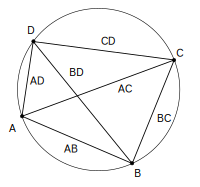
\includegraphics[scale=0.6]{images/tolomeo}
   \caption{El teorema de Tolomeo.}
   \label{fig:Tolomeo}
\end{figure}

\begin{exercise}
	Demuestre el teorema de Tolomeo.
\end{exercise}

Motivados por la astronomía, los árabes también tabularon tablas
trigonométricas hacia fines del siglo VIII. Ellos introdujeron las funciones
circulares y construyeron y perfeccionaron tablas para los valores de la
función seno.  

Grandes avances aparecieron en los siglos IX y X, donde por
ejemplo se logró perfeccionar las tablas de Tolomeo hasta lograr calcular
valores para la función seno con nueve decimales exactos. 

Los indios también tabularon tablas trigonométricas y lo hicieron tabulando
$\sin\theta$.  Medían ángulos en grados, minutos y segundos, ya que usaban la
base 60 de los babilónicos. Por eso, para ellos el valor máximo de la función
seno se alcanzaba aproximadamente en 3438:
\[
	360\times 60=21600=2\pi r
\]
de donde se deduce que $r$ debe ser aproximadamente igual a 3438. Utilizaban 
$3\frac{177}{1250}=3,1416$ como aproximación para el número $\pi$. 

Bhaskhara descubrió una sorprendente aproximación para la función seno, que
lamentablemente no es muy conocida. Si el ángulo $\theta$ se mide en grados y
está entre 0 y 180, se tiene
\[
	\sin\theta\sim \frac{r40(180-\theta)}{40500-\theta(180-\theta)}.
\]
Si traducimos esta fórmula al uso de radianes obtenemos
\[
	\sin x\sim\frac{16x(\pi-x)}{5\pi^2-4x(\pi-x)},\quad 0<x<\pi,
\]
fórmula que, tal como vemos en la figura~\ref{fig:baskhara} da una aproximación
asombrosamente buena.  

No sabemos cómo hizo Bhaskhara para encontrar tal
aproximación, hay muchas posibles explicaciones pero creo que ninguna resulta
del todo convincente. Para el interesado, mas información sobre esta
sorprendente aproximación y una demostración moderna de la fórmula puede
encontrarse en~\cite{MR1108101,MR2793182}.

\begin{figure}[h]
   \centering
   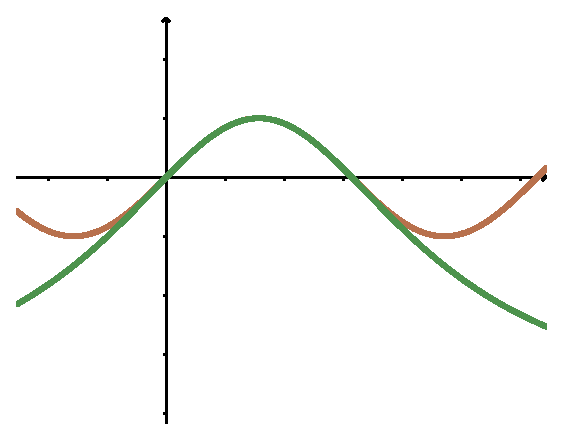
\includegraphics[scale=0.6]{images/baskhara}
   \caption{Una aproximación de Bhaskhara para la función seno.}
   \label{fig:baskhara}
\end{figure}

\index{Aproximación!de Palé}
Es interesante mencionar que la fórmula aproximada encontrada por Bhaskara es
muy similar a la que se obtendría si se utilizara la aproximación de Padé. En
1890, el matemático francés Padé desarrolló una técnica de aproximación de
funciones mediante funciones racionales: si $f$ es una función, $m\geq0$ y
$n\geq1$, se aproxima la función $f$ por una expresión racional de la forma
\[
	g(x)=\frac{a_0+a_1x+a_2x^2+\cdots+a_mx^m}{b_0+b_1x+b_2x^2+\cdots+b_nx^n},
\]
donde los coeficientes $a_0,\dots,a_m$ y $b_0\dots,b_n$ se calculan para que
\[
	f(0)=g(0),\quad
	f'(0)=g'(0),\quad
	f''(0)=g''(0),\quad
	\dots
	\quad
	f^{(m+n)}(0)=g^{(m+n)}(0).
\]
Para mostrar qué tan buena puede llegar a ser esta aproximación concebida por
Palé, mencionamos que la función exponencial $e^x$ puede aproximarse fabulosamente
bien en el intervalo $-1/2\leq x\leq 1/2$ por la función racional
\[
	\frac{120+60x+12x^2+x^3}{120-60x+12x^2-x^3}.
\]

Las aproximaciones de Padé son en general muy buenas y tienen muchas
aplicaciones que involucran cálculos computacionales, ver por
ejemplo~\cite{MR1383091}.  

La idea de aproximar funciones por funciones
racionales había sido ya considerada por Frobenius en un trabajo publicado en
1881.  

Alrededor del año 100 a. C. Menelao publicó un tratado en tres volúmenes donde
aparecen por primera vez los triángulos esféricos y algunas de sus propiedades
más importantes, permitiéndonos reconocer las similitudes y las diferencias que
tienen los triángulos esféricos con los triángulos de la geometría clásica de
Euclides.  Podemos ver un triángulo esférico en la figura~\ref{fig:esferico}.

\begin{figure}[h]
   \centering
   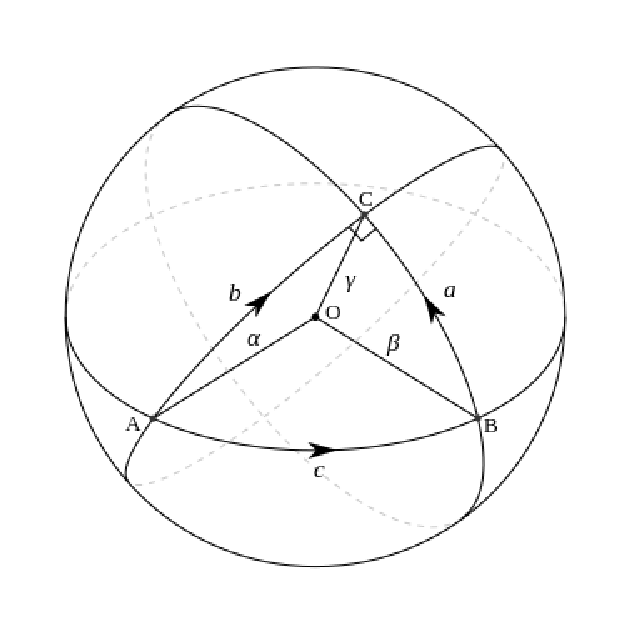
\includegraphics[scale=0.4]{images/esferico}
   \caption{Un triángulo esférico.}
   \label{fig:esferico}
\end{figure}

\index{Teorema!de Menelao}
En el tercero de estos libros aparecen dos resultados que hoy conocemos como teoremas de
Menelao. Estos teoremas no son sino dos versiones, una para la geometría plana y otra para
la geometría esférica, de un mismo resultado sobre triángulos.  En su versión
relativa a la geometría plana, el teorema de Menelao afirma que si se tiene un
triángulo como el que vemos en la figura~\ref{fig:Menelao}, donde vemos una
recta que corta al segmento AB en el punto E, al segmento CB en D y a la
prolongación de la línea AB en el punto F, entonces 
\[
	\frac{EA}{EC}\frac{DC}{DB}\frac{FB}{FA}=1.
\]

\begin{figure}[h]
   \centering
   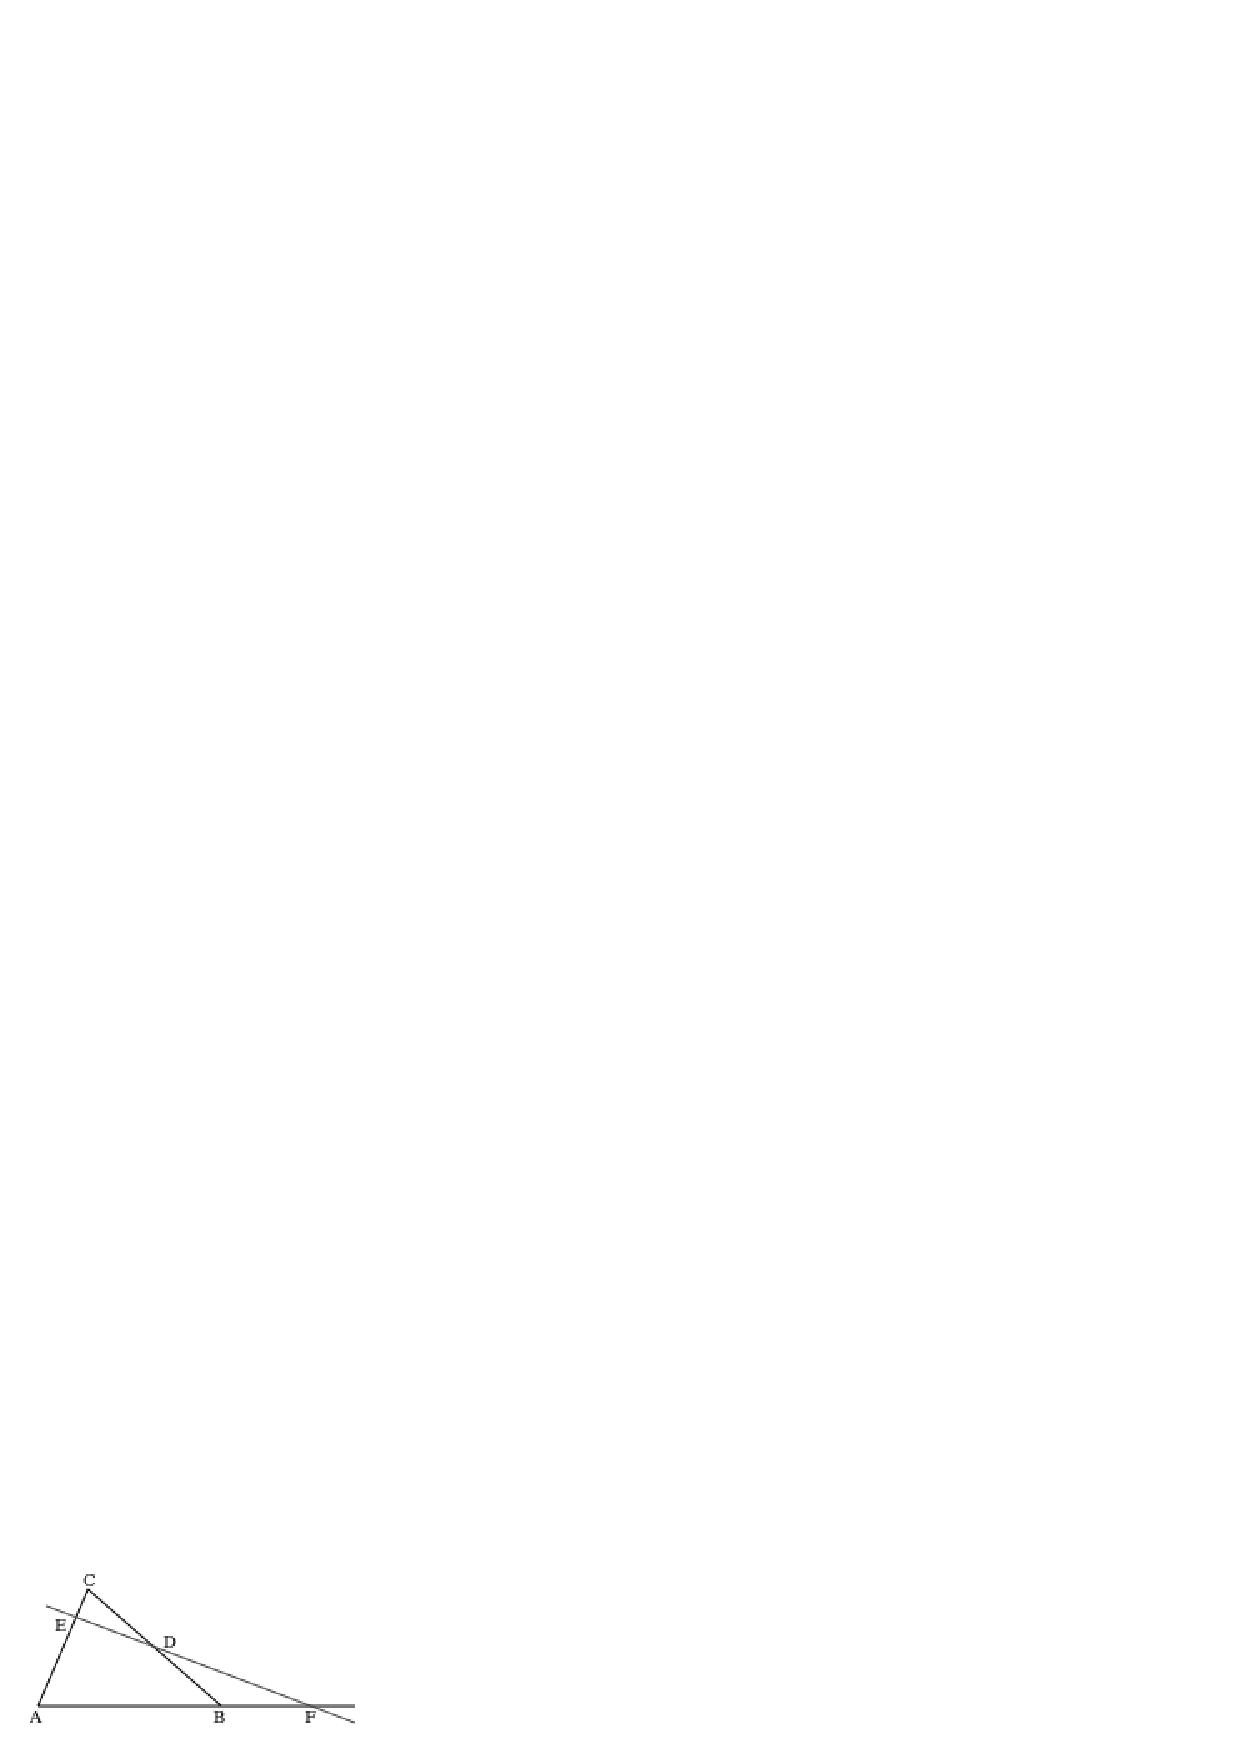
\includegraphics[scale=0.7]{images/menelao}
   \caption{El teorema de Menelao.}
   \label{fig:Menelao}
\end{figure}

\begin{exercise}
	Demuestre el teorema de Menelao.
\end{exercise}

Si bien este resultado de Menelao tiene un análogo en geometría esférica, no
toda la geometría clásica puede adaptarse al contexto esférico. De hecho, tal
como demostró Menelao en el primer volumen, la suma de los ángulos interiores
de un triángulo esférico es siempre mayor a $180$ grados. 

\section*{Las cónicas de Apolonio}

\index{Cónicas}
\index{Elipse}
\index{Hipérbola}
\index{Parábola}
Las \textbf{cónicas} son aquellas curvas que se obtienen al cortar un cono
circular con un plano, tal como vemos en la figura~\ref{fig:conicas}. Las
cónicas son entonces hipérbolas, elipses o parábolas. Vemos una hipérbola en la
figura~\ref{fig:hiperbola}.

\begin{figure}[h]
   \centering
   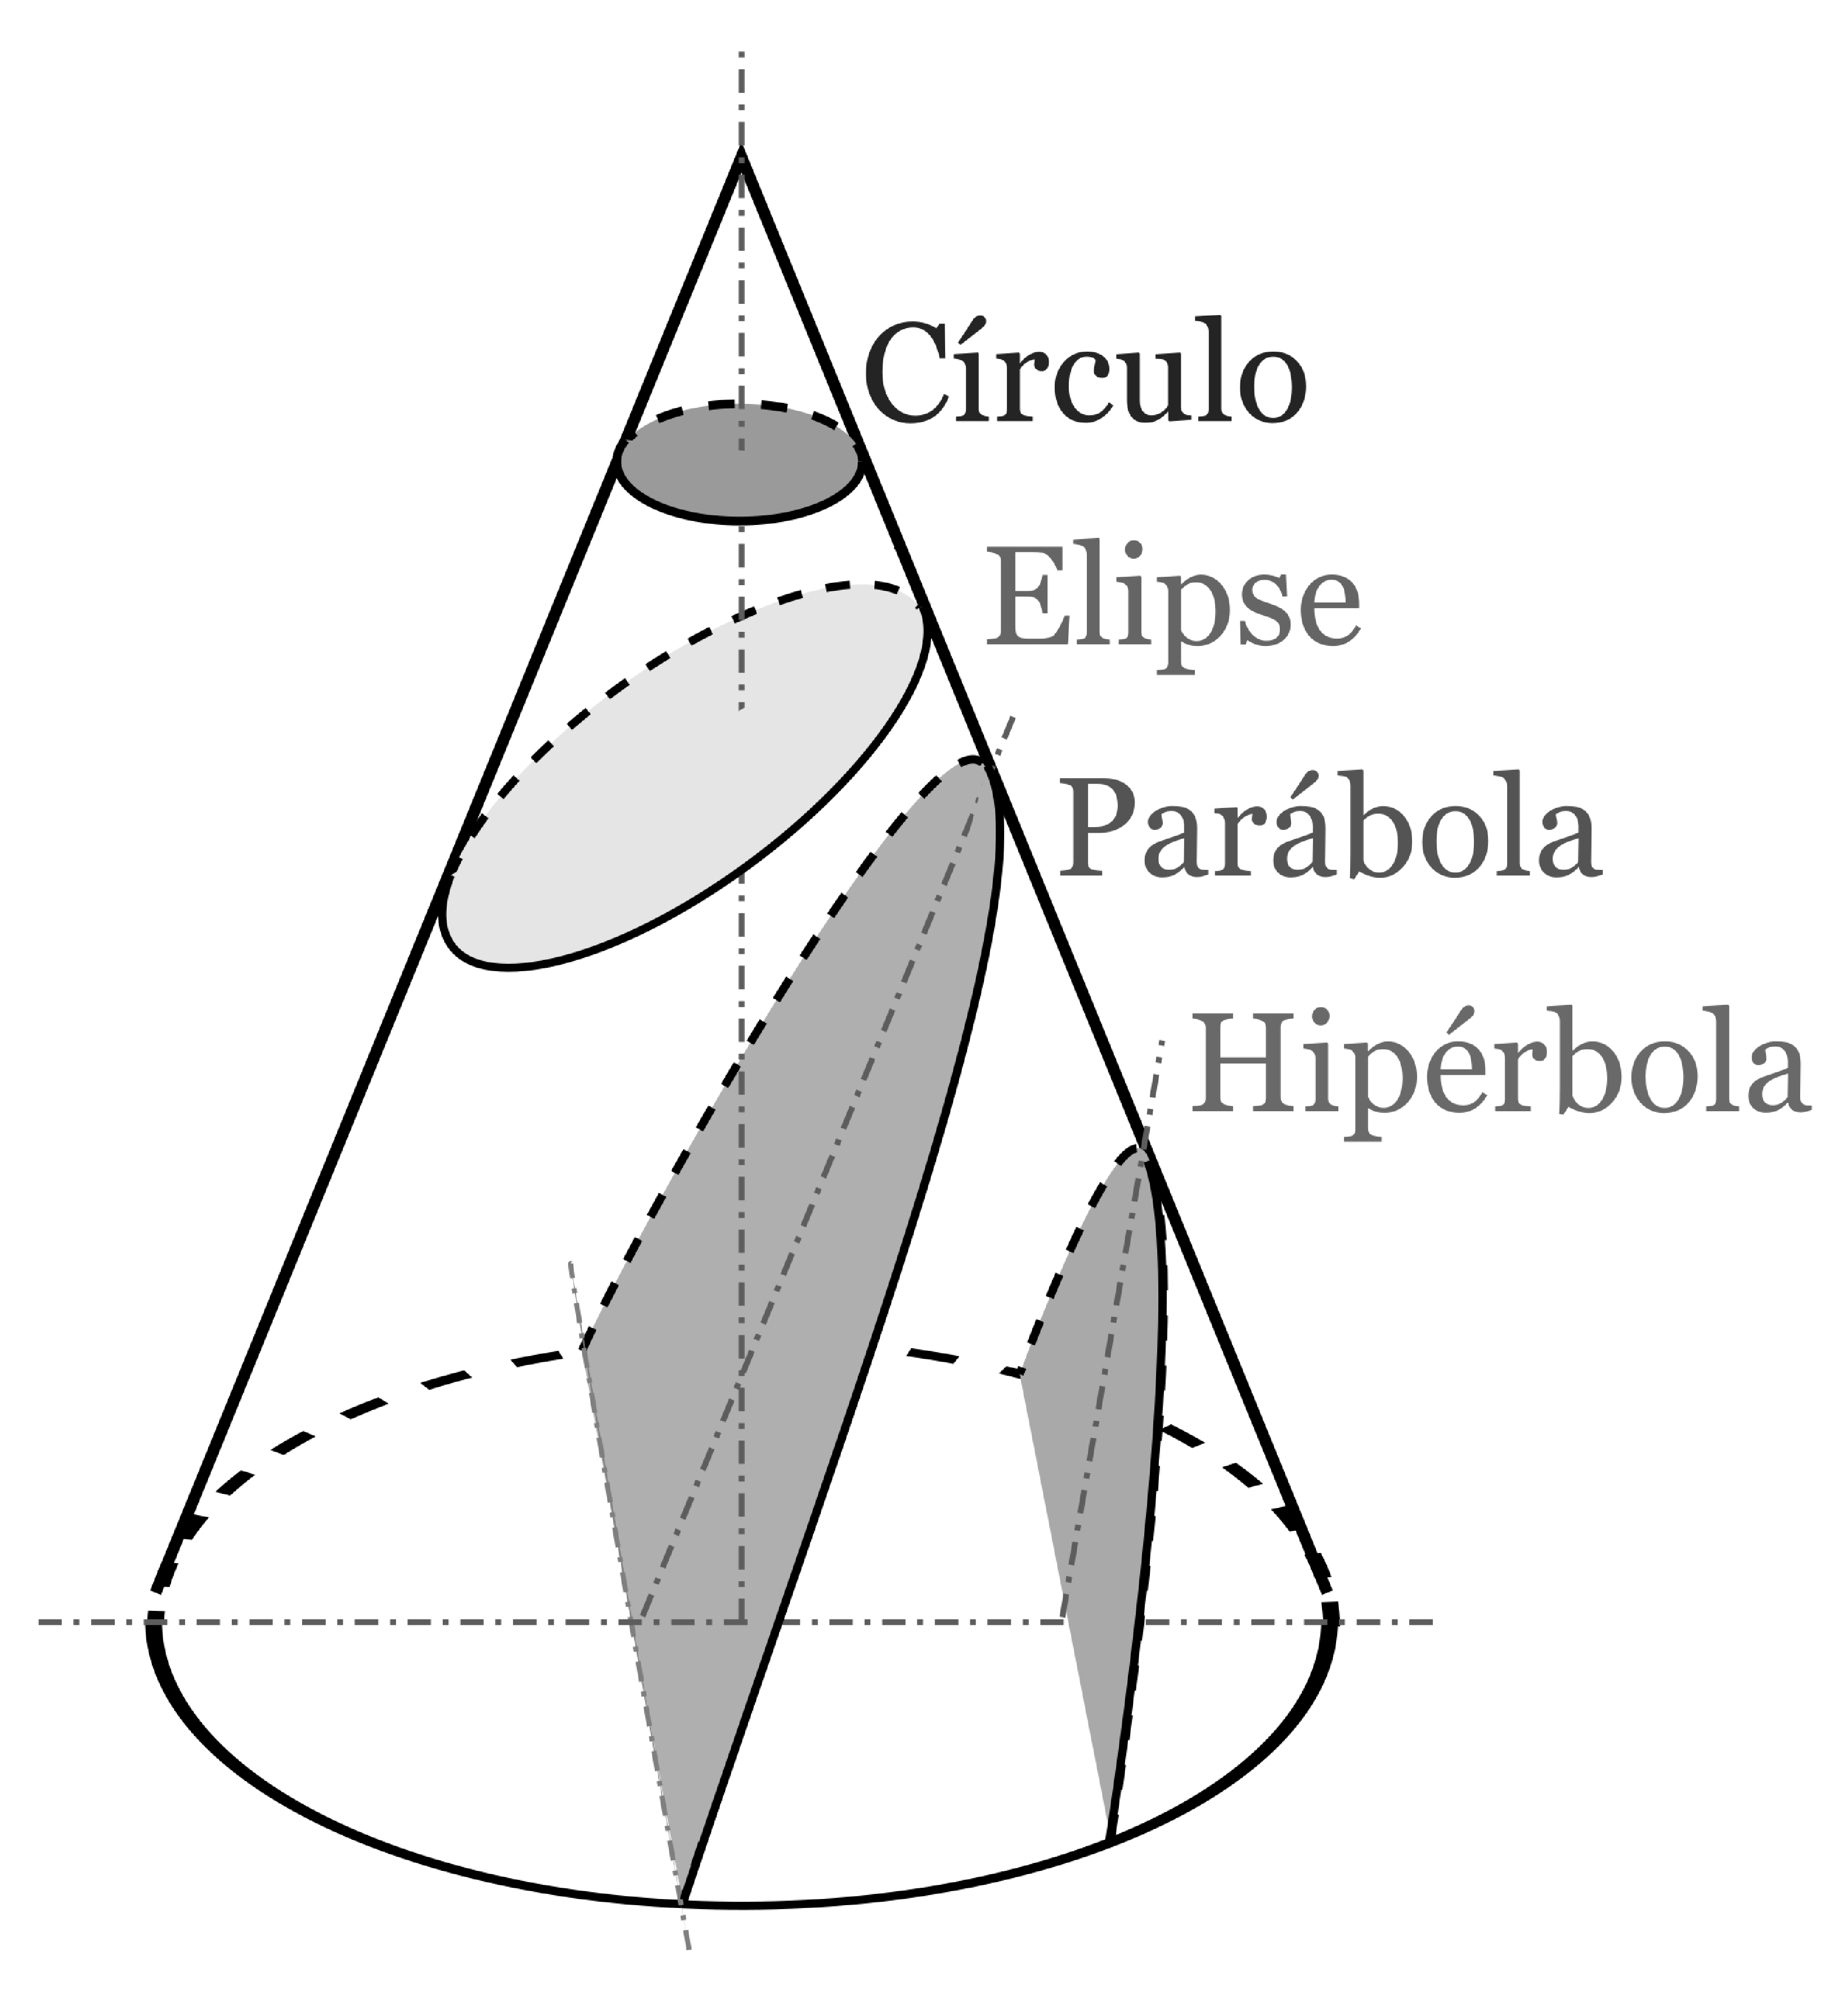
\includegraphics[scale=0.05]{images/conicas}
   \caption{Cónicas.}
   \label{fig:conicas}
\end{figure}

\begin{figure}[h]
   \centering
   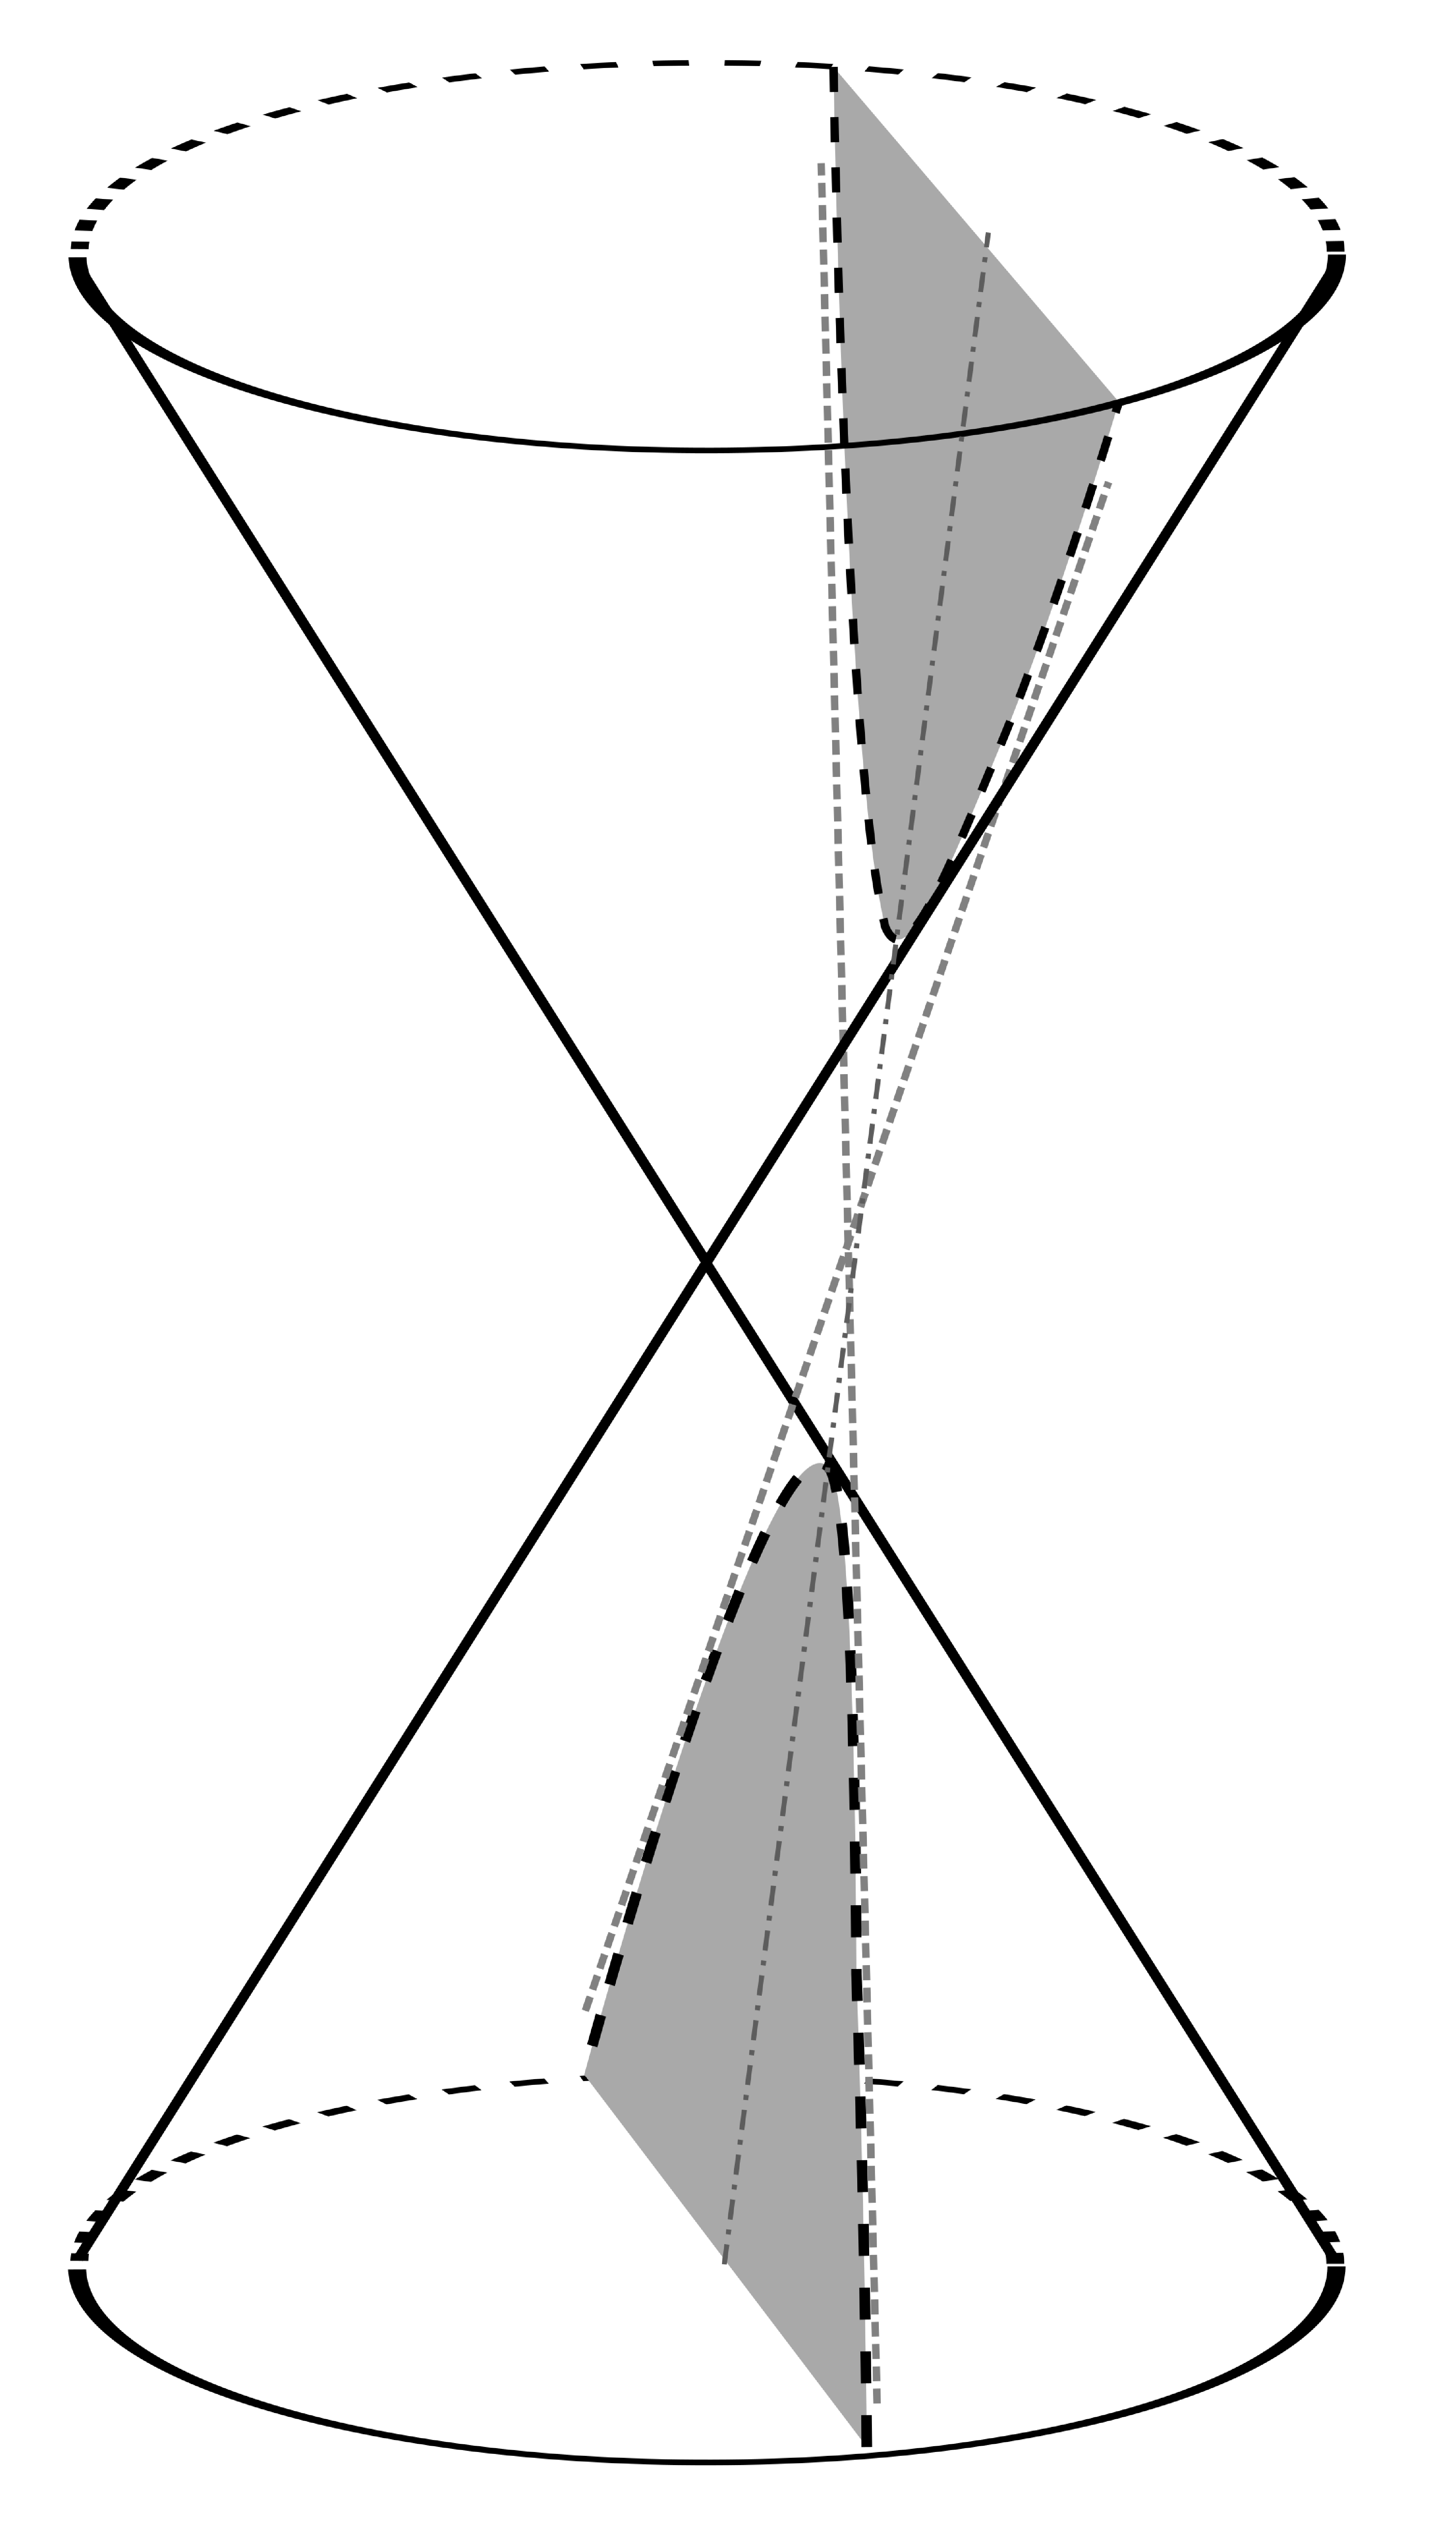
\includegraphics[scale=0.04]{images/hiperbola}
   \caption{Una hipérbola.}
   \label{fig:hiperbola}
\end{figure}

Hoy sabemos que podemos representar cónicas mediante ecuaciones. La
expresión 
\[
	\frac{x^2}{a^2}-\frac{y^2}{b^2}=1
\]
es la ecuación de una hipérbola, la expresión 
\[
	\frac{x^2}{a^2}+\frac{y^2}{b^2}=1
\]
es la ecuación de una elipse y la expresión 
\[	
	y=ax^2
\]
es la ecuación de una parábola. 

Se cree que las cónicas fueron inventadas por Menecmo en épocas de Alejandro
Magno. Originalmente Menecmo utilizó las cónicas para reformular (y en algún
sentido resolver) el famoso problema de la duplicación del cubo. En nuestra
notación, el problema de la duplicación del cubo puede reformularse como el
problema de encontrar la intersección de la parábola $y=\frac12x^2$ con la
hipérbola $xy=1$, ya que esto implica encontrar un $x$ tal que $x^3=2$. Los
griegos aparentemente nunca discutieron sobre los instrumentos necesarios
para dibujar cónicas, aunque sí aceptaron la solución propuesta por Menecmo.
Las ideas de Menecmo sugieren la existencia de un instrumento que resulta ser
una generalización del compás, este instrumento, en forma independiente,
aparece en la matemática árabe del siglo XI. 

El estudio profundo de las cónicas y sus propiedades fhe hecho por Apolonio,
alrededor del año 200 a. C.  Apolonio escribió ocho libros, de los que
conocemos solamente los primeros cuatro en versión original y los tres
restantes mediante traducciones árabes. En la introducción Apolinio escribe
algo que nos permite deducir cómo es que la matemática se transmitía en aquella
época. Los primeros cuatro libros sobre cónicas están dedicados a Eudemo.  Por
la introducción sabemos que Apolinio puso el segundo libro en manos de su hijo
para que él entregara el volumen a Eudemo. Allí le pide que lo lea con cuidado
y que divulgue los resultados allí contenidos a todo aquel que muestre interés.
Pide además a Eudemo que le muestre el libro al geómetra Filónides si llegara a
presentarse la oportunidad. 

%Aparentemente, el geómetra Neucrates tenía en sus manos una versión preliminar
%del tratado de Apolonio. 

Según Apolonio, los primeros cuatro libros forman una introducción elemental,
los restantes versan sobre tópicos más avanzados.  Se estudian propiedades
básicas de las cónicas en el primer libro. En el segundo, se estudian la
hipérbola y sus asíntotas. En el tercero aparecen los focos de la elipse y de
la hipérbola, no así el de la parábola, quizá porque Apolonio no lo consideró
suficientemente interesante, y aparecen además propiedades relativas a los
triángulos y a los cuadrados inscritos y circunscritos (muy posiblemente, estas
propiedades sean las que utilizó Apolonio para estudiar el ``problema de las
tres rectas'' y el ``problema de las cuatro rectas'', algo que aparecerá
después en los trabajos de Pappus). Aparecen además ciertas propiedades métricas
de las cónicas, propiedades que hoy suelen pertenecer a cursos de geometría
proyectiva. Por último, en el cuarto libro se estudian intersecciones y contacto
entre cónicas. En este volumen Apolonio demuestra que dos cónicas no pueden
tener más de cuatro puntos en común. En el quinto libro se estudian las
distancias máxima y mínima de un punto a los puntos de una cónica, resultados
que le dieron fama a Apolonio como geómetra. El sexto libro es quizá menos
importante que el anterior dado que el objetivo principal es el de ordenar y
completar trabajos anteriores, tales como el tratado de Arquímedes sobre
conoides y esferoides. En el libro siete se estudian máximos y mínimos de
ciertas funciones de los diámetros de las cónicas. 

%De hecho, Apolonio está tan ligado a las cónicas como Euclides lo está con sus elementos. 
%Apolonio

Dado que no disponían del álgebra, los griegos no
pudieron estudiar sistemáticamente curvas de grado superior. Sin embargo, sí
fueron capaces de estudiar ciertas curvas particulares sin necesidad de
utilizar ecuaciones que las definan. Un ejemplo notable es la cisoide de
Diocles. 

\section*{Algunas curvas algebraicas}

\index{Curva!algebraica}
Como los griegos no disponían del álgebra, no pudieron profundizar sus
conocimientos sobre curvas, aunque sí pudieron estudiar algunas curvas
algebraicas particulares. Una curva algebraica es una curva dada por los ceros
de un polinomio de dos variables.  Para una digresión histórica sobre la teoría
de curvas algebraicas, referimos al primer capítulo del libro de Brieskorn y
Kn\"{o}rrer \cite{MR2975988}.

\index{Cisoide de Diocles}
Veamos algunos ejemplos de las curvas consideradas en la matemática griega. 
Diocles concibió la curva de hoy conocemos como \emph{cisoide de Diocles} y observó que
esta curva permite duplicar el cubo. Podemos ver una representación gráfica de
esta curva en la figura~\ref{fig:cisoide}. En nuestra notación, esta curva
está representada por la ecuación
\[
	y^2(1+x)=(1-x)^3.
\]

\begin{figure}
   \centering
   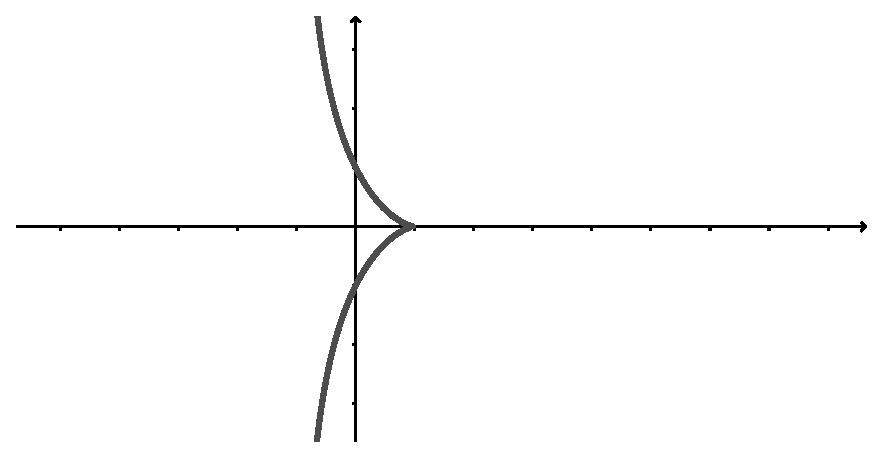
\includegraphics[scale=0.3]{images/cisoide}
   \caption{La cisoide de Diocles.}
   \label{fig:cisoide}
\end{figure}

\index{Toro}
\index{Secciones espíricas}
Los matemáticos griegos conocían algunas superficies. Una de las superficies
que estudiaron es el toro, que es una superficie de revolución tal como la que
podemos ver en la figura~\ref{fig:toro}. 

\begin{figure}
   \centering
   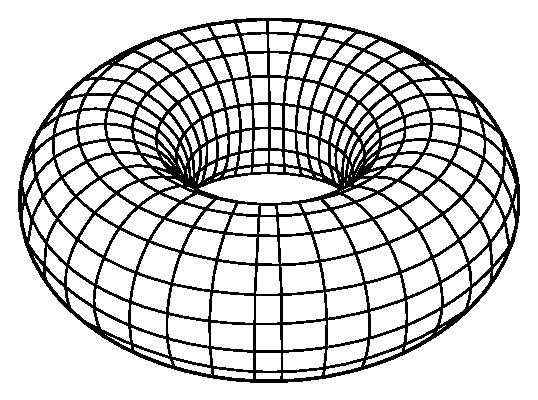
\includegraphics[scale=0.3]{images/toro}
   \caption{El toro.}
   \label{fig:toro}
\end{figure}

Perseo estudió las curvas que se obtienen al cortar el toro
con planos paralelos al eje de rotación, estas curvas se conocen como 
\emph{curvas espíricas}. La ecuación de estas curvas está dada por
\[
	(x^2+y^2)^2=dx^2+ey^2+f.
\]

\begin{figure}
   \centering
   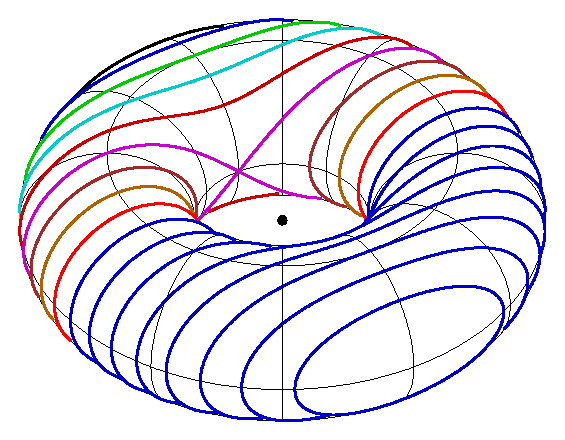
\includegraphics[scale=0.3]{images/spiric}
   \caption{Las curvas espíricas.}
   \label{fig:spiric}
\end{figure}



\index{Lemniscata de Bernoulli}
Algunas de estas curvas fueron redescubiertas en el
siglo XVII gracias a la geometría analítica de Descartes. Un ejemplos notable 
el de la \emph{lemniscata de Bernoulli}, descubierta en 1694 por Jakov Bernoulli. La ecuación 
de esta curva es 
\[
	(x^2+y^2)^2=x^2-y^2
\]
y podemos ver una representación gráfica en la figura~\ref{fig:lemniscata}.

\begin{figure}
   \centering
   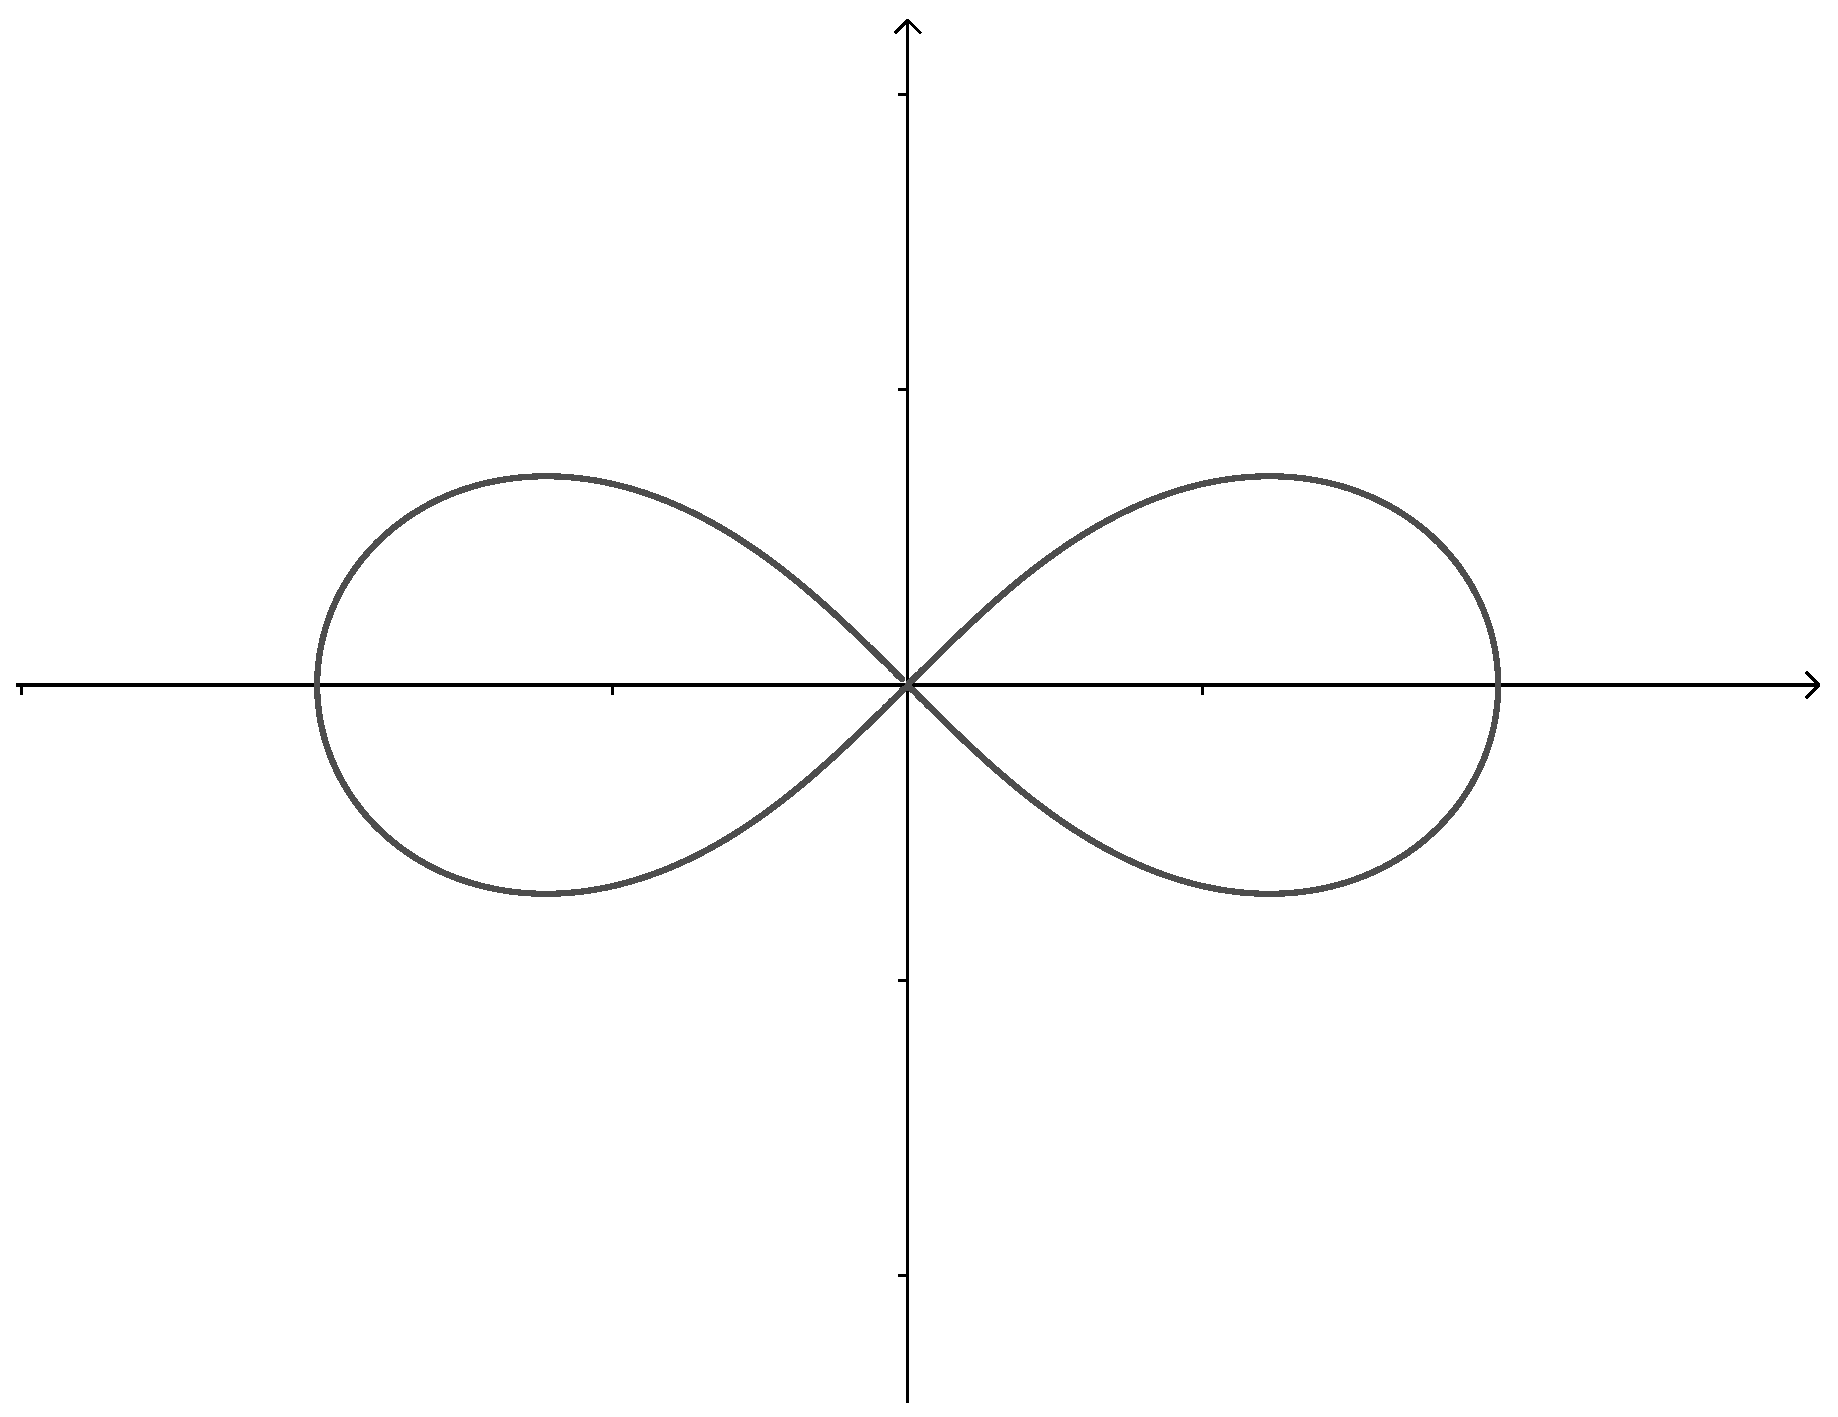
\includegraphics[scale=0.2]{images/lemniscata}
   \caption{La Lemniscata de Bernourlli.}
   \label{fig:lemniscata}
\end{figure}
 
\index{Óvalos de Cassini}
Otro ejemplo es el de los \emph{óvalos de Cassini}, que vemos en la
figura~\ref{fig:Cassini}, y que el astrónomo propuso para reemplazar a las
elipses de Kepler que describen las órbitas planetarias. La lemniscata
es un ejemplo de óvalo de Cassini.

\begin{figure}
   \centering
   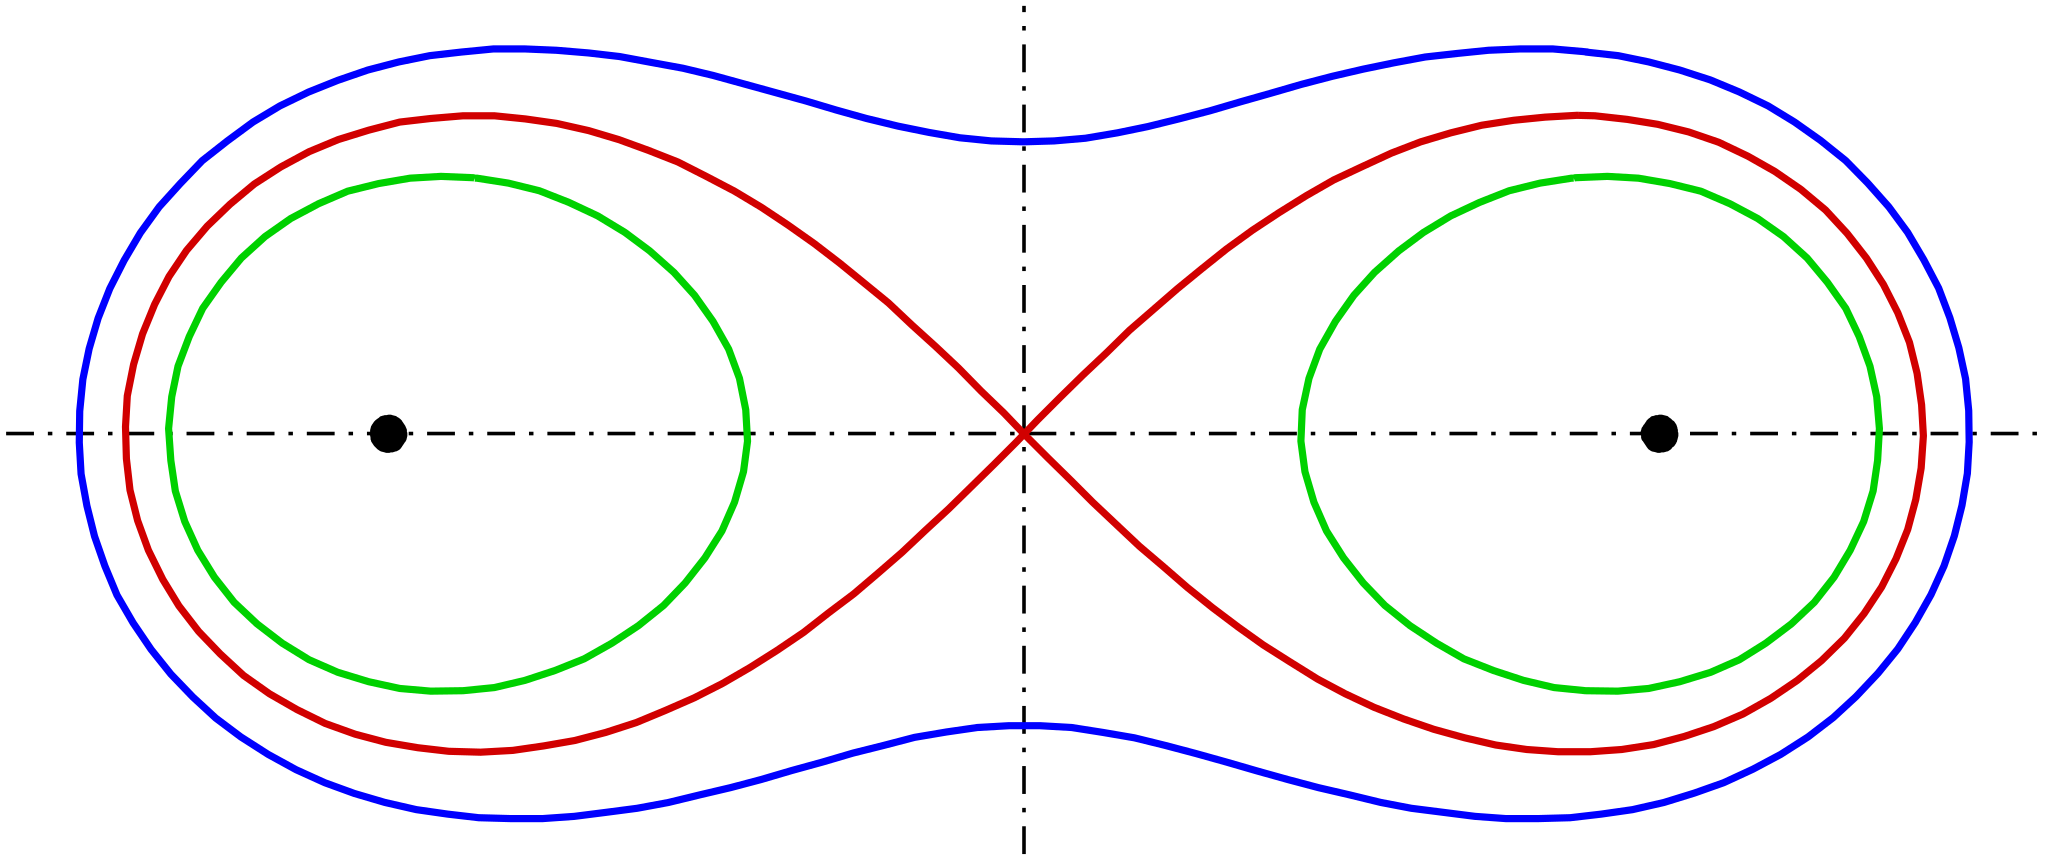
\includegraphics[scale=0.5]{images/cassini}
   \caption{Los óvalos de Cassini.}
   \label{fig:Cassini}
\end{figure}

\index{Epiciclos de Ptolomeo}
\index{Cardioide}
Otra familia de curvas estudiadas por la matemática griega es la de los
epiciclos de Ptolomeo. Estas curvas también tienen sus orígenes en la
astronomía, ya que eran los candidatos naturales a describir las órbitas
planetarias. Un ejemplo de estas curvas es el de la \emph{cardioide} de ecuación
\[
	(x^2+y^2-1)^2=4( (x-1)^2+y^2)
\]
que vemos en la figura~\ref{fig:cardioide}.

\begin{figure}
   \centering
   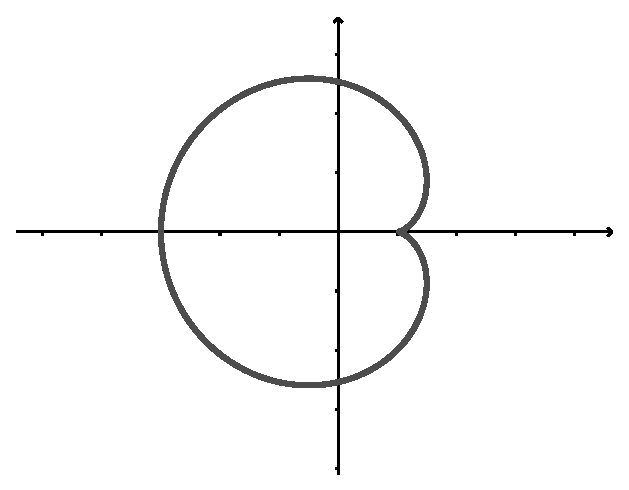
\includegraphics[scale=0.5]{images/cardioid}
   \caption{La cardioide.}
   \label{fig:cardioide}
\end{figure}
 

\chapter{Números y aritmética}

\index{Número!poligonal}
Para los griegos los números tenían propiedades místicas. De hecho, le dieron
mucha importancia --quizá demasiada-- a los números poligonales.  El ejemplo
más famoso de número poligonal es el de los cuadrados. El $25$ es un cuadrado
pues se representa con el siguiente objeto geométrico:
\[
\begin{array}{ccccc}
	\bullet & \bullet & \bullet & \bullet & \bullet\\
	\textcolor{orange}{\bullet} & \textcolor{orange}{\bullet} & \textcolor{orange}{\bullet} & \textcolor{orange}{\bullet} & \bullet\\
	\textcolor{green}{\bullet} & \textcolor{green}{\bullet} & \textcolor{green}{\bullet} & \textcolor{orange}{\bullet} & \bullet\\
	\textcolor{blue}\bullet & \textcolor{blue}{\bullet} & \textcolor{green}{\bullet}     & \textcolor{orange}{\bullet} & \bullet\\
	\textcolor{red}{\bullet} & \textcolor{blue}{\bullet} & \textcolor{green}{\bullet}    & \textcolor{orange}{\bullet} & \bullet
\end{array}
\]

Al observar los colores que usamos en los puntos que forman nuestro cuadrado,
vemos además que podemos escribir al $25$ como $25=1+3+5+7+9$. Esta observación
es un hecho general: la suma de los primeros impares consecutivos siempre será
un cuadrado. Nuestra notación nos permite traducir esta observación en la
identidad 
\[
	1+3+5+\cdots+(2n+1)=(n+1)^2,
\]
que fácilmente puede demostrarse por inducción. 

Similarmente podemos considerar números triangulares: 1, 3, 6, 10\dots
\begin{align*}
	\bullet
	&&
	\begin{array}{cc}
		\bullet\\
		\bullet & \bullet 
	\end{array}
	&&
	\begin{array}{ccc}
		\bullet\\
		\bullet & \bullet \\
		\bullet & \bullet & \bullet
	\end{array}
	&&
	\begin{array}{cccc}
		\bullet\\
		\bullet & \bullet \\
		\bullet & \bullet & \bullet\\
		\bullet & \bullet & \bullet & \bullet
	\end{array}
\end{align*}
Observermos que para calcular el $n$-ésimo núnero triangular $T_n$ lo que
hacemos es sumar los primeros $n$ números: 
\[
	T_n=1+2+3+\cdots+n.
\]
El siguiente gráfico nos permite deducir otra expresión para la fórmula general
que tendrá un número triangular:
\[
	\begin{array}{ccccc}
		\bullet & \textcolor{blue}{\bullet} & \textcolor{blue}{\bullet} & \textcolor{blue}{\bullet} & \textcolor{blue}{\bullet}\\
		\bullet & \bullet & \textcolor{blue}{\bullet} & \textcolor{blue}{\bullet} & \textcolor{blue}{\bullet}\\
		\bullet & \bullet & \bullet & \textcolor{blue}{\bullet} & \textcolor{blue}{\bullet} \\
		\bullet & \bullet & \bullet & \bullet & \textcolor{blue}{\bullet}
	\end{array}
\]
Como el número triangular $T_4$ verifica la ecuación $2T_4=4\times 5$, entonces
$T_4=\frac{4\times 5}{2}$. En general, este mismo argumento nos permite
demostrar que
\[
	T_n=\frac{n(n+1)}{2}.
\]

Uno de los resultados más interesantes sobre (ciertos) números poligonales es el teorema
de Lagrange. Este teorema tiene sus orígenes en los trabajos del matemático
griego Diofanto. Esto motivó a que Bachet, en 1621, 
mientras trabajaba
en una traducción de uno de los libros de Diofanto, conjeturara (o afirmara)
que todo número puede escribirse como suma de a lo sumo cuatro cuadrados. La
primera demostración de este teorema fue dada por Lagrange en 1770.

\begin{theorem}[Lagrange]
	\index{Teorema!de Lagrange}
	\index{Teorema!de los cuatro cuadrados}
	\label{thm:Lagrange}
	Todo número entero positivo es suma de (a lo sumo) cuatro cuadrados.	
\end{theorem}

\begin{proof}
	Como todo entero es producto de números primos, 
	la identidad 
	\begin{equation}
		\begin{aligned}
			\label{eq:Euler}
			(a_1^2+a_2^2+a_3^2+a_4^2)(b_1^2&+b_2^2+b_3^2+b_4^2)\\
			=(a_1 b_1 &+ a_2 b_2 + a_3 b_3 + a_4 b_4)^2\\
			&+(a_1 b_2 - a_2 b_1 + a_3 b_4 - a_4 b_3)^2\\
			&+(a_1 b_3 - a_2 b_4 - a_3 b_1 + a_4 b_2)^2\\
			&+(a_1 b_4 + a_2 b_3 - a_3 b_2 - a_4 b_1)^2
		\end{aligned}
	\end{equation}
	implica que solamente necesitamos demostrar el teorema para los números
	primos. El caso $p=2$ es trivial pues $2=1^2+1^2+0^2+0^2$. Tenemos que
	demostrar entonces el teorema para todo primo impar $p$. 

	\begin{claim}
		Existen $a,b\in\{0,\dots,\frac{p-1}{2}\}$ tales que
		$a^2+b^2+1\equiv0\bmod{p}$. 
	\end{claim}

	Para demostrar la afirmación consideramos los conjuntos 
	\begin{align*}
		A&=\{a^2:a=0,1,\dots,(p-1)/2\},\\
		B&=\{-b^2-1:b=0,1,\dots,(p-1)/2\}.
	\end{align*}
	Como los elementos de $A$ son todos distintos módulo $p$ y los elementos de
	$B$ son también todos distintos módulo $p$, tenemos que $|A|=|B|=(p+1)/2$.
	En consecuencia, $A\cap B\ne\emptyset$. Existen entonces $a\in A$ y $b\in B$
	tales que $0\leq a,b\leq (p-1)/2$ y $a^2=-1-b^2\bmod p$.

	\medskip
	Gracias a la afirmación anterior, sabemos que existe un entero $n\geq1$ tal
	que $a^2+b^2+1=np$. Entonces
	\[
		np=a^2+b^2+1=a^2+b^2+1^2+0^2.
	\]
	es suma de cuatro cuadrados. Sea $m$ el menor entero positivo tal que $mp$
	es suma de cuatro cuadrados, digamos
	\[
		mp=x_1^2+x_2^2+x_3^2+x_4^2.
	\]
	Entonces $1\leq m\leq n<p$. En efecto, si $n\geq p$, como $a$ y $b$ son
	$\leq(p-1)/2$, entonces 
	\[
	p^2\leq np=a^2+b^2+1=2\left(\frac{p-1}{2}\right)^2+1=\frac12(p^2-2p+1)+1,
	\]
	lo que implica que
	$p^2\leq -2p+2$, una contradicción.

	Queremos demostrar que $m=1$. Supongamos
	entonces que $1<m<p$. Si $m$ es par, el número 
	\[
		\frac{m}{2}p=\left(\frac{x_1+x_2}{2}\right)^2
		+\left(\frac{x_1-x_2}{2}\right)^2
		+\left(\frac{x_3+x_4}{2}\right)^2
		+\left(\frac{x_3-x_4}{2}\right)^2
	\]
	es suma de cuatro cuadrados, una contradicción a la minimalidad de $m$. 
	
	Sean ahora $y_1,\dots,y_4$ tales que $x_i\equiv y_i\bmod m$
	y $-m/2<y_i\leq m/2$ para todo $i\in\{1,\dots,4\}$. Como
	\[
		y_1^2+\cdots+y_4^2\equiv x_1^2+\cdots x_4^2= mp\equiv 0\bmod m,
	\]
	existe un entero $r\geq0$ tal que $mr=y_1^2+\cdots+y_4^2$. 
	
	\begin{claim}
		$r\in\{1,\dots,m-1\}$. 
	\end{claim}

	Si $r=0$, entonces $y_1=y_2=y_3=y_4=0$. Luego $m$ divide a cada $x_i$ y
	entonces $m^2$ divide a cada $x_i^2$. En consecuencia, 
	\[
		m^2\mid x_1^2+\cdots+x_4^2=mp,
	\]
	una contradicción pues $m\nmid p$ y $m\ne1$. Como entonces $r\geq 1$, 
	\[
		mr=y_1^2+\cdots+y_4^2\leq 4\left(\frac{m}{2}\right)^2=m^2
	\]
	y luego $r\leq m$. Para ver que $r\ne m$ basta observar que si $r=m$, 
	entonces 
	\[
		m^2=y_1^2+\cdots+y_4^2\leq (m/2)^2+(m/2)^2+(m/2)^2+(m/2)^2=m^2,
	\]
	y luego cada $y_j$ tomará el máximo valor posible, es decir
	$y_1=y_2=y_3=y_4=m/2$. En particular, $m$ es un número par, una contradicción. 

	\medskip
	La identidad \ref{eq:Euler} nos permite escribir
	\[
		m^2rp=(mp)(mr)=(x_1^2+\cdots+x_4^2)(y_1^2+\cdots+y_4^2)=z_1^2+\cdots+z_4^2.
	\]
	Como $x_i\equiv y_i\bmod m$ para todo $i\in\{1,\dots,4\}$, entonces 
	$z_i\equiv 0\bmod m$ para todo $i\in\{1,\dots,4\}$. Por ejemplo,
	\[
	z_1=x_1y_1+x_2y_2+x_3y_3+x_4y_4\equiv x_1^2+x_2^2+x_3^2+x_4^2\equiv 0\bmod m.
	\]
	Similarmente, $z_i\equiv0\bmod m$ para todo $i\in\{2,3,4\}$. 
	
	Para cada $i\in\{1,\dots,4\}$ sea
	$w_i=z_i/m\in\Z$. Entonces 
	\[
		rp=w_1^2+w_2^2+w_3^2+w_4^2,
	\]
	una contradicción a la minimalidad de $m$.
\end{proof}

La identidad~\eqref{eq:Euler} fue descubierta por Euler; figura en una carta
que le escribió a Goldbach el 4 de mayo de 1748.

\begin{exercise}
    Demuestre la identidad \eqref{eq:Euler}. 
\end{exercise}

La identidad \eqref{eq:Euler} fue
redescubierta por Hamilton en 1843 en sus trabajos sobre cuaterniones. Una
manera sencilla y elegante de demostrar esta identidad (u otra más o menos similar) se basa en que el
determinante es una multiplicación multiplicativa y que vale además la
siguiente fórmula:
\[
	(x_1^2+x_2^2+x_3^2+x_4^2)^2=\det\begin{pmatrix}
		x_1 & x_2 & x_3 & x_4\\
		-x_2 & x_1 & -x_4 & x_3\\
		-x_3 & x_4 & x_1 & -x_2\\
		-x_4 & -x_3 & x_2 & x_1.
	\end{pmatrix}.
\]
Alrededor de 1840 Graves y Cayley descubrieron independientemente una identidad
similar que involucra suma de ocho cuadrados. 

\begin{exercise}
	Demuestre que todo número $n>169$ puede escribirse como suma de exactamente
	cinco cuadrados positivos.
\end{exercise}

\index{Fórmula!de Jacobi}
En 1828 Jacobi dio una fórmula sorprendente que permite calcular con exactitud
la cantidad $r_{4}(n)$ de representaciones del entero $n$ como suma de cuatro
cuadrados:
\[
	r_{4}(n)=8(2+(-1)^n)\sum_{\substack{d\mid n\\2\nmid d}}d.
\]

\index{Suma!de tres cuadrados}
No todo número puede representarse como suma de tres cuadrados.  Los primeros
numeros que pueden representarse como suma de exactamente cuatro cuadrados son 
\[
	7, 15, 23, 28, 31, 39, 47, 55, 60, 63, 71\dots
\]
La sucesión de tales números lleva el código \href{https://oeis.org/A004215}{A004215}.

En 1798 Legendre demostró el siguiente resultado:

\begin{theorem}[Legendre]
\index{Teorema!de Legendre}
Un entero positivo $n$ puede representarse como suma de tres
cuadrados si y sólo si no es de la forma $n=4^a(8b+7)$. 
\end{theorem}

No vamos a demostrar el teorema de Legendre, pero vamos a utilizarlo 
para demostrar el teorema de Lagrange: Si $n$ es un
entero positivo, escribimos $n=4^{\alpha}m$, donde $m$ es un entero no
divisible por $4$. Si $m\equiv k\bmod 8$ para algún $k\in\{1,2,3,5,6\}$,
entonces $m$ es suma de tres cuadrados y el resultado queda demostrado. En caso
contrario, $m-1$ es también suma de tres cuadrados y luego $m$ es suma de
cuatro cuadrados. 

% otra demo con geometría de números?


% Escribimos $n-169=x_1^2+\cdots+x_4^2$ como suma de cuatro cuadrados, donde
% podemos suponer sin perder generalidad que $x_1\geq x_2\geq x_3\geq x_4\geq
% 0$. Si todos los $x_j$ son positivos, no hay nada para demostrar pues
% $169=13^2$. Si $x_4=0$, entonces escribimos $169=5^2+12^2$ y el resultado
% queda también demostrado. Si $x_3=x_4=0$, entonces usamos que
% $169=12^2+4^2+3^2$. Por último, si $x_2=x_3=x_4=0$, usamos que
% 169=10^2+8^2+2^2+1^2$. 

El teorema de Legendre también permite además demostrar fácilmente el siguiente
teorema de Gauss:

\begin{theorem}[Gauss]
	\index{Teorema!de Gauss}
	Todo entero positivo es suma de tres números triangulares.
\end{theorem}

\begin{proof}
	Por el teorema de Legendre, todo entero de la forma $8n+3$ puede expresarse
	como suma de tres cuadrados, digamos $8n+3=a_1^2+a_2^2+a_3^2$. Como los
	cuadrados módulo ocho son 0, 1 y 4, cada $a_i$ es un número impar. Como 
	\begin{align*}
		8n+3&=(2x+1)^2+(2y+1)^2+(2z+1)^2\\
		&=4(x(x+1)+y(y+1)+z(z+1))+3,
	\end{align*}
	entonces tenemos que 
	\[
		n=\frac{x(x+1)}{2}+\frac{y(y+1)}{2}+\frac{z(z+1)}{2}.\qedhere
	\]
\end{proof}

Este teorema aparece en los diarios de Gauss con fecha del 10 de julio de 1796
y su demostración fue publicada en \emph{Disquisitiones Arithmeticae}.  

El Gauss y el teorema de Lagrange sobre suma de cuatro cuadrados son
casos particulares de un resultado más general, conjeturado por Fermat en 1638
y demostrado por Cauchy en 1813. 

\begin{theorem}[Cauchy]
\index{Teorema de Cauchy}
\label{thm:Cauchy}
    Sea $m\geq3$. Todo entero positivo puede
    expresarse como una suma de $m+2$ números $(m+2)$-poligonales.
\end{theorem}

Puede demostrarse que los números
$(m+2)$-poligonales se definen mediante la fórmula
\[
	p_m(k)=\frac{mk(k-1)}{2}+k.
\]

En el caso $m=1$ la fórmula da números triangulares pues
\[
	p_1(k)=\frac{k(k+1)}{2}.
\]
En cambio, si 
$m=2$, la fórmula da los números cuadrados pues
\[
p_2(k)=k(k-1)+k=k^2
\]

\begin{exercise}
	Demuestre que los números pentagonales son de la forma
	$\displaystyle{\frac{3k^2-k}{2}}$. 
\end{exercise}

Una demostración
breve y sencilla del teorema de Cauchy fue descubierta por Nathanson en
1987~\cite{MR866422}.

Otro resultado interesante sobre números poligonales es teorema de Euler. 
En 1750 Euler demostró que
\[
	\prod_{n=1}^\infty(1-x^n)=1+\sum_{k=1}^\infty (-1)^k\left(x^{(3k^2-k)/2}+x^{(3k^2+k)/2}\right).
\]
El teorema de Lagrange sobre cuatro cuadrados y esta fórmula de Euler son ahora
parte de una rama de la teoría de números conocida como
\emph{la teoría de funciones theta}, rama que desarrolló Jacobi en 1830. 

\section*{El problema de Waring}

El teorema de Lagrange admite varias direcciones generalizaciones posibles. En
1770 Waring afirmó en sus \emph{Meditationes Algebraic\ae} que todo número es
suma de $\leq 4$ cuadrados, $\leq 9$ cubos, $\leq 19$ potencias cuartas, y, en
general, $\leq g(k)$ potencias $k$-ésimas, donde $g(k)$ depende únicamente de
$k$ y no del número que se está representando. Waring no tenía una demostración
sino que hizo esas afirmaciones únicamente basado en limitada evidencia
numérica. 

Si existe $s\in\Z_{\geq1}$ tal que todo número es suma de $\leq s$ potencias
$k$-ésimas, entonces también valdrá que todo número es suma de $\leq t$
potencias $k$-ésimas para todo $t\geq s$. Tiene sentido entonces definir $g(k)$
como el menor $s\in\Z_{\geq1}$ tal que 
\[
	x_1^k+\cdots+x_s^k=n
\]
admite solución en los enteros positivos para todo $n$. El siguiente
resultado fue demostrado en 1772 por Johannes Euler, hijo del famoso
matemático: 

\begin{theorem}[Euler]
	\index{Teorema!de Euler}
	$g(k)\geq 2^k+\lfloor (3/2)^k\rfloor-2$. 
\end{theorem}

\begin{proof}
	Primero observemos que para escribir al entero $n=2^k\lfloor
	(3/2)^k\rfloor-1$ como suma de potencias $k$-ésimas, necesitamos al menos
	$2^k+\lfloor (3/2)^k\rfloor-2$ sumandos. En efecto, si $q=\lfloor
	(3/2)^k\rfloor$, entonces
	\[
		n=2^kq-1\leq 2^k(3/2)^k-1<3^k.
	\]
	Si $n=x_1^k+\cdots+x_{g(k)}^k$, entonces $x_j\in\{0,1,2\}$ para todo
	$j\in\{1,\dots,g(k)\}$ y además 
	\[
		n=2^kq-1=\underbrace{(2^k+\cdots+2^k)}_{q\text{-veces}}-1=\underbrace{(2^k+\cdots+2^k)}_{(q-1)\text{-veces}}+2^k-1.
	\]
	Como además 
	\[
		2^k-1=\underbrace{1^k+\cdots+1^k}_{(2^k-1)\text{-veces}},
	\]
	se tiene la cota que buscamos.
\end{proof}

La constante 
\[
	I(k)=2^k+\lfloor (3/2)^k\rfloor-2 
\]
tiene interés en el estudio del problema de Waring. En 1853 Bretschneider
conjeturó que $g(k)=I(k)$ para todo $k\geq2$.

\begin{exercise}
	\index{Teorema!de Lagrange}
	Demuestre que $g(2)=4$. 
\end{exercise}

Entre 1909 y 1912 Wieferich y Kempner demostraron que $g(3)=I(3)=9$.  La
primera demostración de este resultado fue de Wieferich, pero contenía algunos
errores que posteriormente fueron reparados por Kempner.    
En 1940 Pillai
demostró que $g(6)=I(6)=73$ y en 1964 Jing--Jung Chen demostró que
$g(5)=I(5)=37$.  
El caso de los bicuadrados es bastante más difícil: entre 1986
y 1992 Balasubramanian, Deshouillers y Dress demostraron que $g(4)=I(4)=19$.
Entre 1936 y 1990 varios matemáticos contribuyeron a calcular el valor exacto
de $g(k)$ para $7\leq k\leq 471000000$. En todos estos casos, $g(k)=I(k)$.
Veamos algunos de estos valores:
\begin{align*}
	&g(7)=I(7)=143,
	&&g(8)=I(8)=279,
	&&g(9)=I(9)=548.
\end{align*}
Otros valores de $g(k)$ pueden encontrarse en la sucesión
\href{https://oeis.org/A002804}{A002804}.

En general es muy difícil calcular con exactitud el valor de $g(k)$. Nos
contentaremos con mostrar algunas cotas en ciertos casos particulares, que en
realidad es lo único que se necesita si se quiere demostrar algún caso
particular del problema de Waring.

\begin{theorem}[Liouville]
	\index{Teorema!de Liouville}
	$g(4)\leq 53$.
\end{theorem}

\begin{proof}
	Es fácil demostrar que
	\begin{equation}
		\label{eq:Lucas}
		6(x_1^2+x_2^2+x_3^2+x_4^2)^2=\sum_{1\leq i<j\leq 4}(x_i+x_j)^4+\sum_{1\leq i<j\leq 4}(x_i-x_j)^4
	\end{equation}
	Dado $n\in\Z_{\geq1}$ escribimos $n=6q+r$ con $0\leq r\leq 5$. Por el teorema de Lagrange podemos
	escribir a $q$ como suma de cuatro cuadrados:
	\[
		n=6(x_1^2+x_2^2+x_3^2+x_4^2)+r=6x_1^2+6x_2^2+6x_3^2+6x_4^2+r.
	\]
	La identidad~\eqref{eq:Lucas} nos dice que todo número de la forma $6y^2$
	es suma de doce potencias cuartas, y entonces $n-r$ es suma de 48 potencias
	cuartas. Como $0\leq r\leq 5$, vemos que $r$ es suma de $\leq 5$ potencias
	cuartas, se concluye que para escribir al entero $n$ vamos a necesitamos
	$\leq 48+5=53$ potencias cuartas.
\end{proof}

\index{Identidad!de Lucas}
\index{Identidad!de Liouville}
La identidad~\eqref{eq:Lucas} fue descubierta por Lucas en 1876, la identidad
usada por Liouville para demostrar que $g(4)\leq53$ es un poco más complicada y
es la identidad que se obtiene de~\eqref{eq:Lucas} con $x_1=y_1+y_2$,
$x_2=y_1-y_2$, $x_3=y_3+y_4$, $x_4=y_3-y_4$.

No es difícil convencerse de que las identidades como la que vimos
en~\eqref{eq:Lucas} son importantes para atacar el problema de Waring. Se hace
necesario tener una mejor notación. Escribiremos entonces 
\[
	(x_1\pm x_2\pm\cdots\pm x_m)^k=\sum(x_1+\epsilon_2x_2+\cdots+\epsilon_mx_m)^k
\]
donde la suma se toma sobre todas las posibles elecciones de  
$\epsilon_j\in\{-1,1\}$ para $2\leq j\leq m$. Por ejemplo:
\[
	(x_1\pm x_2)^4=(x_1+x_2)^4+(x_1-x_2)^4.
\]
La identidad~\eqref{eq:Lucas} que usamos para demostrar que $g(4)\leq 53$ puede
escribirse entonces abreviadamente como
\[
	6(x_1^2+x_2^2+x_3^2+x_4^2)^2=\sum_{i<j}(x_i\pm x_j)^4,
\]
donde además resultará de utilidad recordar que la suma involucrada tiene
además ocho términos.

El problema de Waring comenzó a acercarse a una solución definitiva cuando 
en 1908 Hurwitz observó que la existencia de una identidad polinomial
de la forma
\[
	p(x_1^2+\cdots+x_4^2)^k=\sum_{i=1}^N p_i(a_{1i}x_1+a_{2i}x_2+a_{3i}x_3+a_{4i}x_4)^{2k}
\]
donde $p,p_1,p_2,p_3,p_4\in\Z_{\geq1}$ y $(a_{ij})\in\Z^{N\times 4}$, permite
demostrar que 
\[
	g(2k)\leq g(k)(p_1+\cdots+p_N)+p-1,
\]
de donde evidentemente se obtiene que si $g(k)$ es finito, también lo será
$g(2k)$. 

\begin{theorem}[Hurwitz]
	\index{Teorema!de Hurwitz}
	$g(8)\leq 44793$. 
\end{theorem}

\begin{proof}
	Vamos a utilizar la identidad polinomial
	\begin{equation}
	\label{eq:Hurwitz}
	\begin{aligned}
		5040(x_1^2+x_2^2+x_3^2+x_4^2)^4= \sum_{1\leq i\leq 4}6x_i^8
		&+\sum_{1\leq i<j\leq 4}60(x_i\pm x_j)^8\\
		&+ \sum_{1\leq i<j<k\leq 4}(2x_i\pm x_j\pm x_k)^{8}\\
		&+\sum_{1\leq i<j<k<l\leq 4}6(x_i\pm x_j\pm x_k\pm x_l)^{8}.
	\end{aligned}
	\end{equation}
	Observemos que la primera suma del miembro derecho tiene cuatro términos,
	la segunda tiene doce términos, la tercera tiene 48 términos y la cuarta
	tiene ocho términos.  La identidad~\eqref{eq:Hurwitz} nos dice entonces que
	todo número de la forma $5040q^4$ es suma de 
	\[
		6\times 4+12\times 60+48+8\times 6=840
	\]
	potencias octavas. Como además demostramos que todo número es suma de
	$g(4)\leq 53$ potencias cuartas, tenemos que todo $n\geq 5040$ puede
	escribirse como suma de $840\times g(4)\leq 840\times 53=44520$ potencias
	cuartas. Por otro lado, si $n<5040$, entonces siempre podremos escribir a
	$n$ como suma de $\leq 273$ potencias octavas (pues $3^8=6561>5039)$. Luego 
	$g(8)\leq 840g(4)+273\leq 44793$.
\end{proof}

\index{Teorema!de Hilbert--Waring}
En 1909 Hilbert demostró que aquellas identidades propuestas por Hurwitz
siempre existen. Con eso logró entonces obtener una demostración completa al
problema de Waring.  Muchos matemáticos simplificaron la complicada demostración
original de Hilbert: Haursdoff, Stridsberg, Hurwitz, Remak y Frobenius. En la
demostración de Hilbert no aparecen cotas explícitas para $g(k)$. En 1953
Rieger usó las ideas de Hilbert y logró demostrar que 
\[
	g(k)\leq (2k+1)^{260(k+3)^{3k+8}}.
\]

Hoy en día la demostración que dio Hilbert en 1909 no es sino apenas una
curiosidad. Es cierto que después de hacer algunas modificaciones a los
argumentos de Hilbert tales como las que hizo Rieger uno puede obtener cotas
para $g(k)$, pero mucho mejores cotas pueden obtenerse gracias a métodos
analíticos. Un método analítico muy poderoso con el que puede resolverse
el problema de Waring fue divisado por Hardy y Littlewood en 1920 y se conoce
como el \emph{método del círculo} de Hardy--Litlewood. 

\section*{Números perfectos}

\index{Número!perfecto}
Otros números que tuvieron cierto interés en épocas pasadas fueron los números
perfectos. Un entero positivo se dice \textbf{perfecto} si es igual a la suma
de sus divisores propios positivos. Veamos algunos ejemplos:
\begin{align*}
	6 &= 1+2+3,\\
	28 &= 1+2+4+7+14,\\
	496 &= 1 + 2 + 4 + 8 + 16 + 31 + 62 + 124 + 248.
\end{align*}

Otros ejemplos de números perfectos aparecen en la sucesión
\href{https://oeis.org/A000396}{A000396}.


En el libro IX Euclides demostró que si $p$ es un número primo tal que $2^p-1$
es primo, entonces $n=2^{p-1}(2^p-1)$ es un número perfecto. 

\begin{exercise}
	Demuestre el teorema de Euclides sobre números perfectos.
\end{exercise}

En el siglo XVIII
Euler demostró el recíproco del resultado de Euclides: cada número perfecto par
$n$ es de la forma $n=2^{p-1}(2^p-1)$ donde $p$ y $2^{p}-1$ son números primos. 

\begin{exercise}
	Demuestre el teorema de Euler sobre números perfectos.
\end{exercise}

\begin{exercise}
	Demuestre que un número perfecto par es siempre un número triangular. 
\end{exercise}

\begin{exercise}
	Demuestre que un número perfecto par es siempre un número binomial.
\end{exercise}

Hasta el siglo XV se conocían muy pocos números perfectos.  En 1603 el
matemático italiano Pietro Cataldi encontró los siguientes números perfectos: 
\[
	2^{16}(2^{17} - 1) = 8 589 869 056,\quad
	2^{18}(2^{19} - 1)= 137 438691 328. 
\] 

Al momento se conocen únicamente 51 números perfectos. El mayor de los
perfectos conocidos hasta el momento\footnote{Septiembre de 2019} es un número
de 49724095 dígitos:
\[
	2^{82 589 932} (2^{82 589 933} - 1)
\]
y fue encontrado en diciembre de 2018.

No se sabe si existen finitos números perfectos y no se conocen números
perfectos impares.  

En 2012, Ochem y Rao demostraron que no existen números
perfectos impares de orden $<10^{1500}$. 

\section*{Números primos}

Como bien señala Weil en~\cite{MR734177}, el amor del hombre por los números es
quizá aún más antiguo que la teoría de números.  

\index{Número!primo}
Los griegos consideraban a los números primos como números que no admiten
representaciones rectangulares.  Los primeros números primos son
\[
    2, 3, 5, 7, 11, 13, 17, 19, 23, 29, 31, 37, 41, 43, 47, 53, 59, 61, 67, 71, 73, 79\dots
\]
La sucesión de números primos es \href{https://oeis.org/A000040}{A000040}.

El teorema fundamental de la aritmética afirma que todo número puede escribirse
como producto de números primos y esa escritura es esencialmente única. Este
resultado no aparece explícitamente en los libros de Euclides, aunque hay
muchos resultados del libro VII que son casi equivalentes. Tampoco aparece en
\emph{Essai sur la Théorie des Nombres}, famoso tratado escrito por Legendre de
1798 sobre teoría de números. La primera aparición precisa junto con una
demostración rigurosa figura en el famoso \emph{Disquisitiones arithmeticae} de
Gauss de 1801. 

Euclides demostró en la proposición 20 del libro IX que existen infinitos
números primos. 

\begin{quote}
	Hay más números primos que cualquier cantidad propuesta de números primos.
\end{quote}
La demostración es bien conocida y no la reproduciremos aquí. Sí mencionaremos,
en cambio, que la demostración de Euclides revela que la existencia de una
sucesión de enteros positivos coprimos dos a dos, implicará la infinitud de los
números primos. En efecto, si $a_1,a_2,\dots$ es una sucesión de enteros
coprimos dos a dos y para cada $j$ se toma un primo $p_j$ que divide al
elemento $a_j$, entonces los $p_j$ serán todos distintos.

Recordemos que los números de Fermat son los enteros de la forma
\[
	F_n=2^{2^n}+1.
\]
En un una carta que Goldbach le escribió a Euler en julio de 1730, se demuestra
que los números de Fermat son coprimos dos a dos. Este resultado da entonces
una demostración alternativa de la infinitud de los números primos.

\begin{theorem}(Goldbach)
	\index{Teorema!de Goldbach}
	Los numeros de Fermat son coprimos dos a dos.
\end{theorem}

\begin{proof}
	Se demuestra fácilmente por inducción que $F_n-2=F_0F_1\cdots F_{n-1}$ vale
	para todo $n\in\N$. Si $m<n$, entonces $F_m$ divide a $F_n-2$. Si $p$ es un
	número primo tal que $p\mid F_n$ y $p\mid F_m$, entonces $p\mid F_n-2$ y
	luego $p\mid 2$, una contradicción pues $F_m$ es un número impar. 
\end{proof}

Veamos otra demostración muy breve y elegante, aparentemente encontrada por Hermite:

\begin{quote}
Para cada $n\geq0$ sea $q_n$ el menor número primo que divide a $n!+1$. Como
$q_n>n$, se concluye que el conjunto $\{q_n:n\geq1\}$ contiene infinitos elementos.
\end{quote}
Esta demostración es particularmente interesante. Calculemos algunos
términos de la sucesión $(q_n)$:
\[
	2,2,3,7,5,11,7,71,61,19\dots
\]
Es la sucesión \href{https://oeis.org/A051301}{A051301}.

\begin{exercise}
	Demuestre que todo número primo pertenece a la sucesión $(q_n)$.
\end{exercise}

%Es interesante mencionar que al día de hoy no se sabe la sucesión $n!+1$
%contiene infinitos números primos. Los primos de esta forma son 
%\[
% 1, 2, 3, 4, 6, 7, 11, 12, 14\dots
%\]
%y 
%aparecen en la sucesión \verb+A088054+.

Existen muchas otras demostraciones de la infinitud de los números primos. 
Euler dio varias demostraciones distintas de este hecho. Demostró la infinitud
de los primos al observar, por ejemplo, que el producto
\[
	\prod_{p}\frac{p}{p-1}
\]
es infinito. La ``demostración'' de Euler es más o menos así: sea
\[
	x=1+\frac12+\frac13+\frac14+\cdots
\]
Calculamos 
\[
	\frac{x}{2}=\frac12+\frac14+\frac16+\cdots
\]
y restamos para obtener
\[
	\frac{x}{2}=1+\frac13+\frac15+\frac17+\frac19+\cdots
\]
Hacemos ahora algo similar: dividimos por tres y restamos par obtener:
\[
	\frac12\frac23x=1+\frac15+\frac17+\cdots=\sum_{\substack{n\geq1\\(n:6)=1}}\frac1n,
\]
donde la suma se toma sobre todos los enteros positivos coprimos con seis. Al
continuar con este procedimiento, Euler obtiene la expresión
\[
	\prod_p\frac{p}{p-1}
	=\frac{(1\cdot 2\cdot 4\cdot 6\cdot 10\cdots)}{(2\cdot 3\cdot 5\cdot 7\cdot 11\cdots)}x=1
\]
y concluye entonces que, como $x$ es infinito (pues la serie armónica diverge),
el producto $\prod p/(p-1)$ también debe ser infinito. En conclusión, existen
infinitos números primos. La demostración de Euler carece del rigor necesario,
aunque hay que mencionar que los problemas que presenta pueden arreglarse. De
hecho, entre 1875 y 1876 Kronecker arregló esta demostración de Euler y la
expuso en sus clases sobre la teoría de los números primos.

En 1737 Euler dio una demostración alternativa de la infinitud de los números
primos. Lo hizo al demostrar que la serie
\[
	\frac12+\frac13+\frac15+\frac17+\frac{1}{11}+\frac{1}{13}+\frac{1}{17}+\cdots=\sum_{p}\frac{1}{p},
\]
donde la suma se toma sobre todos los números primos, diverge. La falta de
rigor en la demostración original de Euler puede arreglarse fácilmente. Daremos
la demostración de este resultado encontrada por Clarkson en 1966:

\begin{theorem}[Euler]
	\index{Teorema!de Euler}
	La serie $\sum_{p}\frac{1}{p}$ diverge. 
\end{theorem}

\begin{proof}
	Supongamos que la serie fuera convergente. Existe entonces un entero positivo $k$ tal que 
	\[
		\sum_{m=k+1}^{\infty}\frac{1}{p_m}<\frac12.
	\]
	Sea $Q=p_1\cdots p_k$. Para cada $n\geq1$ consideramos el número $1+nQ$.
	Como ningún primo $p_j$ con $j\in\{1,\dots,k\}$ divide a $1+nQ$, los
	factores primos de $1+nQ$ están todos en el conjunto $\{p_{k+1},p_{k+2}\dots\}$. Para cada $N\geq1$, 
	\[
		\sum_{n=1}^N\frac{1}{1+nQ}\leq \sum_{t=1}^\infty\left(\sum_{m=k+1}^{\infty}\frac{1}{p_m}\right)^t
	\]
	pues la suma del miembro derecho contiene a todos los términos que aparecen
	en la suma del miembro izquierdo. Como además 
	\[
		\sum_{n=1}^N\frac{1}{1+nQ}\leq \sum_{t=1}^\infty\left(\sum_{m=k+1}^{\infty}\frac{1}{p_m}\right)^t<\sum_{t=1}^\infty\left(\frac12\right)^t<\infty,
	\]
	obtenemos la convergencia de la serie 
	\[
		\sum_{n=1}^{\infty}\frac{1}{1+nQ}\geq\sum_{n=1}^\infty\frac{1}{n(1+Q)}=\frac{1}{1+Q}\sum_{n=1}^\infty\frac{1}{n},
	\]
	una contradicción, pues sabemos que la serie $\sum_{n=1}^\infty\frac{1}{n}$ diverge.
\end{proof}

Hasta el momento, los siete mayores números primos conocidos son primos de Mersenne. 
Desde 1997 todos los primos de Mersenne descubiertos se hicieron dentro del
proyecto GIMPS. Este proyecto de cálculo distribuido fue creado por George
Woltman en 1996 y tiene como objetivo buscar números primos de Mersenne. GIMPS
es uno de los primeros proyectos de cálculo distribuido y es notablemente
exitoso: de los 50 primos de Mersenne conocidos, los últimos 17 encontrados
fueron dentro de este proyecto.  El mayor primo de Mersenne conocido hasta el
momento es 
\[
	2^{82589933}-1
\]
y tiene 24862048 dígitos; fue descubierto en diciembre de 2018. Este número es
además el mayor número primo que se conoce. 

Hoy en día los números primos son importantes no solo en matemática pura sino
en la criptografía. Muchos de los algoritmos de encriptación utilizados se
basan en el uso de números primos. 

Desde mucho tiempo atrás existe un profundo interés en conocer cómo se
distribuyen los números primos. Basados en una tabla de primos $\leq10^6$
similar a la que vemos en la tabla~\ref{tab:pi}.

\begin{table}[h!]
  \begin{center}
    \caption{Algunos valores para $\pi(x)$.}
    \label{tab:pi}
    \begin{tabular}{r|r|r|r} 
	  \hline
	  $x$ & $\pi(x)$ & $x/\log x$ & $\pi(x)/(x/\log x)$\\
      \hline
	  $10$ & 4 & 4,3 & 0,93\\
	  $10^2$ & 25 & 21,5 & 1,15\\
	  $10^3$ & 168 & 144,9 & 1,16\\
	  $10^4$ & 1229 & 1086 & 1,11\\
	  $10^5$ & 9592 & 8686 & 1,10\\
	  $10^6$ & 78498& 72464 & 1,08\\
	  \hline
    \end{tabular}
  \end{center}
\end{table}

Gauss y Legendre conjeturaron independientemente el teorema del número primo.
La fórmula de Legendre para aproximar a la cantidad $\pi(x)$ de primos $\leq x$
es la siguiente:
\[
	\pi(x)\sim \frac{x}{\log x},
\]
que quiere decir que 
\[
	\lim_{n\to\infty} \frac{\pi(x)}{(x/\log x)}=1.
\]
La fórmula de Gauss es equivalente, aunque bastante mejor que la de Legendre: 
\[
	\pi(x)\sim\operatorname{Li}(x)=\int_2^x\frac{dt}{\log t}.
\]
Por ejemplo:
\[
	\pi(10^7)=664579,\quad
	\pi(10^7)-\frac{10^7}{\log(10^7)}=44158,\quad
	\pi(10^7)-\operatorname{Li}(10^7)=339.
\]
Veamos otro ejemplo, aún más sorprendente: 
\begin{align*}
	&\pi(10^{10})=455052511,\\
	&\pi(10^{10})-\frac{10^{10}}{\log (10^{10})}=20758029,\\
	&\pi(10^{10})-\operatorname{Li}(10^{10})=3104.
\end{align*}


Durante muchos años los matemáticos intentaron en vano demostrar estos
resultados sobre la distribución de los números primos.  En 1859, Riemann atacó
el problema con métodos analíticos y encontró una sorprendente conexión entre
los números primos y la función de variable compleja 
\[
\zeta(s)=\sum_{n\geq1}1/n^{s}. 
\]
Esta función hoy se conoce como la \textbf{función zeta de Riemann} y es de
fundamental importancia en la matemática moderna. De hecho, uno de los
problemas más importantes de la matemática, que se conoce como la hipótesis de
Riemann, es una conjetura sobre la distribución de los ceros de la función
$\zeta(s)$. 

El teorema del número primo fue demostrado independiente por de la Valle
Poussin y por Hadamard en 1896; en ambos casos, la demostración se basa en el
estudio de propiedades analíticas de la función de variable compleja
$\zeta(s)=\sum_{n\geq1}1/n^{s}$. 

En 1949, Selberg e Erd\"os encontraron,
independientemente, una demostración elemental del teorema del número primo.
Esta demostración elemental generó mucho revuelo en la comunidad matemática y
muchas discusiones entre Erd\"os y Selberg, ya que ambos, de alguna forma,
consideraban merecer el crédito de haber encontrado una demostración elemental
del teorema del número primo.  Cabe aclarar que cuando nos referimos a una
demostración elemental, nos referimos a una demostración que solamente utiliza
técnicas básicas, aunque en general sean demostraciones muy difíciles de
entender. Es importante recordar lo siguiente: demostración elemental no quiere
significa sencilla y fácil de entender. 

Uno de los resultados más importantes de la teoría de números durante el siglo
XIX es el siguiente teorema, demostrado por Dirichet entre 1837 y 1839: Si $k$
y $l$ son enteros coprimos, entonces existen infinitos números primos
congruentes a $l$ módulo $k$. 
Este resultado fue enunciado en forma explícita por Euler en 1785 en el caso
$l=1$ y por Legendre en 1798 en el caso general. La segunda edición del libro
de Legendre sobre teoría de números, publicada en 1808, incluye una
demostración incorrecta de este resultado sobre números primos. El error está
en creerse que un cierto lema es fácil de demostrar, tal como afirmaba
Legendre.  Dirichlet fue uno de los primeros en observar que aquel lema no era,
en realidad, fácil de demostrar. En 1858 Dupré demostró que aquel lema de
Legendre era en realidad falso.

Existe además una versión del teorema del número primo para progresiones
aritméticas: la cantidad de primos $p\leq x$ congruentes a $l$ módulo $k$ es
asintóticamente igual a 
\[
	\frac{1}{\phi(k)}\pi(x).
\]

En la teoría de los números primos podemos encontranos con muchos resultados
que son consecuencia de propiedades matemáticas muy profundas, y
simultáneamente podemos también encontrarnos que resultados que difícilmente
puedan interpretarse como algo más que una curiosidad.  

En la correspondencia
entre Euler y Goldbach podemos encontrarnos con el siguiente hecho notable: El
polinomio 
\[
	x^2-x+41
\]
da un número primo para todo $x\in\{0,\dots,40\}$. Similarmente, el polinomio
\[
	x^2-79x+1601
\]
da un número primo para todo $x\in\{0,\dots,79\}$. 

En 1752 Goldbach demostró,
aunque con algunas deficiencias fácilmente reparables, el siguiente resultado:

\begin{theorem}[Goldbach]
	\index{Teorema!de Goldbach}
	No existe $f\in\Z[X]$ de grado $n\geq1$ tal que $f(n)$ es primo para todo
	$n\in\N$.
\end{theorem}

\begin{proof}
	Sea $f\in\Z[X]$ no constante tal que $f(n)$ es un número primo para todo
	$n\in\N$. Fijemos $x_0\in\N$. Como $f(x_0)\not\in\{-1,0,1\}$, existe
	entonces un primo $p$ tal que $p$ divide a $f(x_0)$. Como
	\[
		f(x_0+mp)\equiv f(x_0)\equiv 0\bmod p
	\]
	para todo $m\in\Z$, se tiene entonces que $f(x_0+mp)\in\{-p,p\}$ para todo
	$m\in\Z$, una contradicción.
\end{proof}

Entre las curiosidades matemáticas que involucran números primos tenemos, por
supuesto, las fórmulas explícitas. 

\begin{exercise}
	\index{Teorema!de Wilson}
	Demuestre que un entero $p$ es primo si y sólo si
	$(p-1)!\equiv -1\mod p$. 
\end{exercise}

El resultado del ejercicio anterior se conoce como el teorema de Wilson.
Aparentemente, el resultado era conocido por el matemático árabe Alhazen,
alrededor del año 1000. Waring conocía el enunciado, y también Wilson, su
estudiante. Sin embargo, ninguno de los dos pudo demostrarlo. La primera
demostración es de 1771 y fue encontrada por Lagrange. Es posible de Leibniz
conociera este resultado, pero nunca lo publicó.

% Una demostración de Gauss bien fácil utiliza el teorema de Fermat. La saqué de Davenport, página 4X. 


\begin{exercise}
	Demuestre que la función 
	\[
		n\mapsto \left\lfloor\frac{n!\bmod (n+1)}{n}\right\rfloor (n-1)+2.
	\]
	genera todos los números primos, donde
	$\lfloor x\rfloor$ denota la parte entera de $x$. 
\end{exercise}

Estos dos ejercicios nos muestran que existen fórmulas para encontrar números
primos, pero son absolutamente ineficientes y no pueden usarse en aplicaciones
serias. En esta misma dirección, mencionaremos un resultado demostrado por
Mills en 1946:

\begin{theorem}[Mills]
	Existe un número real $A$ tal que $\lfloor A^{3^n}\rfloor$ es un número
	primo para todo $n\in\N$.	
\end{theorem}

\begin{proof}
	Para la demostración necesitamos utilizar el siguiente resultado demostrado
	por Ingham en 1937: Si $p_n$ denota al $n$-ésimo número primo, existe una
	constante $K$ tal que 
	\[
		p_{n+1}-p_n\leq Kp_n^{5/8}.
	\]

	\begin{claim}
		Si $N>K^8$, entonces existe un primo $p$ tal que $N^3<p<(N+1)^3-1$. 
	\end{claim}

	Para demostrar esta afirmación, sea $p_n$ el mayor número primo mayor que
	$N^3$. Como $N>K^8$, entonces $N^{1/8}>K$ y luego
	\[
		N^3<p_{n+1}<p_n+Kp_n^{5/8}<N^3+KN^{15/8}<N^3+N^2<(N+1)^3-1.
	\]

	Sea $P_0$ un número primo tal que $P_0>K^8$. La afirmación anterior nos
	permite construir una sucesión $P_0,P_1,P_2\dots$ de primos tales que
	\[
		P_n^3<P_{n+1}<(P_n+1)^3-1.
	\]
	Sean 
	\[
		u_n=P_n^{3^{-n}},\quad
		v_n=(P_n+1)^{3^{-n}}.
	\]
	Vamos a demostrar que la sucesión $u_1,u_2\dots$ converge. Para eso veremos que es monótona y acotada. 
	Primero observamos que, como 
	\begin{align*}
		&u_{n+1}=P_{n+1}^{3^{-n-1}}>P_n^{3^{-n}}=u_n,
	\end{align*}
	la sucesión $(u_n)_{n\in\N}$ tiene límite pues es monótona y acotada. 
	Sea $A=\lim_{n\to\infty}u_n$. Como además 
	\begin{align*}
		&v_n=(P_n+1)^{3^{-n}}>P_n^{3^{-n}}=u_n,\\
		&v_{n+1}=(P_{n+1}+1)^{3^{-n-1}}<(P_n+1)^{3^{-n}}=v_n,
	\end{align*}
	se tiene que
	$u_n<A<v_n$ para todo $n$. Luego $P_n<A^{3^n}<P_n+1$ para todo $n$ y el
	teorema queda demostrado al tomar parte entera pues $\lfloor
	A^{3^n}\rfloor=P_n$. 
\end{proof}

El resultado anterior no tiene aplicaciones prácticas. No se conoce el valor
real de la constante $A$ del teorema; de hecho, ni siquiera se sabe si $A$ es
un número racional. Sin embargo, si se asume la veracidad de la hipótesis de
Riemann, puede demostrarse que $A$ es aproximadamente igual a
\[
	1.3063778838630806904686144926\dots
\]
Tampoco se conocen los primos que produce la función de Mills. Si se asume la
veracidad de la hipótesis de Riemann puede demostrarse que los primeros primos
producidos por la función de Mills son
\[
    2,11,1361,2521008887, 16022236204009818131831320183\dots
\]
Estos números son los elementos de la sucesión
\href{https://oeis.org/A051254}{A051254}.

Es natural preguntarse si puede demostrarse algún resultado similar al de Mills
pero sin apelar al profundo teorema de Ingham. 

\begin{exercise}
	Si existen constantes $\beta<1$, $A$ y $c$ tales que para cualesquiera dos primos
	consecutivos $p_{n-1}<p_n$ tales que $A<p_{n-1}$ se tiene que
	$p_n-p_{n-1}<cp_{n-1}^\beta$, entonces para todo $\alpha>\frac{1}{1-\beta}$
	existe un número real $\theta$ tal que 
	\[
		\lfloor \theta^{\alpha^n}\rfloor 
	\]
	es primo para todo $n\in\N$.
\end{exercise}

En 1845 Bertrand conjeturó que dado $n\geq1$ siempre existe un número primo $p$
tal que $n<p<2n$.  Si bien Bertrand pudo comprobar que la conjetura era cierta
para todo $n\leq 3\times 10^6$, no pudo demostrarlo para todo $n$. La conjetura
fue demostrada completamente por Chebyshev en 1852. Ramanujan encontró una
demostración más sencilla que la encontrada por Chebyshev en 1919.  En 1932
Erd\"os dio una demostración incluso más sencilla y completamente elemental que
utiliza solamente propiedades de los números combinatorios. 

En 1951 Wright demostró que existe $\alpha\in\R$ tal que si $g_0=\alpha$ y
$g_{n+1}=2^{g_n}$, entonces $\lfloor g_n\rfloor$ es siempre un número primo. La
demostración de este resultado puede consultarse en~\cite{MR43805}; es similar
a la demostración que hicimos del teorema de Mills, aunque el teorema de Ingham
será reemplazado por el teorema de Bertrand--Chebyshev.


\section*{La conjetura de Goldbach}

\index{Constante!de Brun}
\index{Pentium FDIV bug}
\index{Nicely, Thomas}
\index{Teorema!de Brun}
La \textbf{conjetura de Goldbach} afirma que todo entero par mayor que dos
puede expresarse como suma de dos primos. Por ejemplo:
\[
	10=3+7,\quad
	18=5+13,\quad
	20=7+13,\quad
	90=43+47.
\]
Una versión de esta conjetura aparece en una carta del 7 de junio de 1742 que
Goldbach le escribió a Euler. Aparentemente esta conjetura era conocida desde
tiempo antes; en los trabajos póstumos de Descartes puede encontrarse una
afirmación similar a la conjetura de Goldbach: no está demostrado pero todo
número puede escribirse como suma de uno, dos o tres números primos.

A pesar de los esfuerzos de muchos matemáticos, la conjetura permanece abierta. 

Gracias a cálculos computacionales se sabe que la conjetura es verdadera para
números menores que $4\times 10^{17}$. En 1937 Vinogradov demostró que todo
número impar suficientemente grande es suma de tres números primos. En 1948
Rényi demostró que existe un entero $M$ tal que cada número impar $n$
suficientemente grande es suma de un primo y otro número que tiene a lo sumo
$M$ factores primos. Si alguien pudiera demostrar que $M=1$, se tendría
entonces la veracidad de la conjetura de Goldbach. En 1966 Jing-Run demostró
que $M\leq 2$. 

Recientemente pudo demostrarse una versión débil de la conjetura de Goldbach:
Todo número impar mayor que cinco puede expresarse como suma de tres números
primos.  Esta conjetura es la \textbf{conjetura débil de Goldbach}. Es fácil
demostrar que la veracidad de la conjetura de Goldbach implicaría la veracidad
de la versión débil de la conjetura.  La conjetura débil apareció publicada sin
demostración por primera vez en 1770 en el tratado \emph{Meditationes
algebraicae}, escrito por el matemático inglés Edward Waring. Fue demostrada
por el matemático peruano Harald Helfgott en 2013. 

\section*{La infinitud de los primos gemelos}

Dos números primos $p$ y $q$ son números \textbf{primos gemelos} si $|p-q|=2$.
Los primeros ejemplos son
\[
	(3, 5), (5, 7), (11, 13), (17, 19), (29, 31), (41, 43),\dots
\]

La sucesión de primos gemelos es 
\href{https://oeis.org/A077800}{A077800}.

En 2009 se demostró que los números 
\[
	65516468355\times 2^{333333}+1,
	\quad
	65516468355\times 2^{333333}-1,
\]
son primos gemelos; cada uno de estos números tiene 100355 dígitos.  Hasta
ahora no se descubrieron primos gemelos mayores. Este par de primos se encontró
dentro del proyecto de cálculo distribuido PrimeGrid, desarrollado por Rytis
Slatkevi\v{c}ius.  Se tardó más de dos años en encontrar este par de primos y
en esta tarea colaboraron 18661 personas. Según el reporte oficial, una única
computadora de escritorio hubiera tardado cerca de dos siglos en encontrar
estos números.

\begin{exercise}
	Utilice el teorema de Wilson y 
	demuestre que los enteros $n$ y $n+2$ son primos gemelos si y sólo si
	\[
		4( (n-1)!+1)\equiv -n\bmod{n(n+2)}.
	\]
\end{exercise}

Desde hace mucho tiempo se conjetura que existen infinitos primos gemelos. 

En 1919 Brun demostró que la serie
\[
	\sum\left(\frac1p+\frac1{p+2}\right)=\left(\frac13+\frac15\right)+\left(\frac15+\frac17\right)+\left(\frac1{11}+\frac1{13}\right)+\cdots,
\]
donde la suma se toma sobre todos los primos $p$ tales que $p+2$ es también un
número primo, es convergente. 

En 1994, mediante el cálculo de los primos
gemelos menores que $10^{14}$ el matemático estadounidense Thomas Nicely
determinó que la serie converge a 
\[
1,9021605777\dots,
\]
número que hoy se conoce
como la \textbf{constante de Brun}. Fue durante este cálculo que Nicely
descubrió un problema en los procesadores Pentium, hoy conocido como el
``Pentium FDIV bug''. La prestigiosa revista Science publicó un artículo en
1995 que describe la importancia de los problemas de teoría de números para
descubrir problemas como el que encontró Nicely.  Después del incidente Intel,
acabó cooperando con Nicely para testear los nuevos microprocesadores.

En 2013 Zhang demostró que existe un entero $N$ tal que existen infinitos pares
de primos cuya diferencia es $N$; el entero $N$ es aproximadamente igual a
$70\times10^6$.  Este trabajo tuvo gran repercusión, ya que no se conocían
resultados de este tipo desde tiempos de Euclides.  Después de la publicación
del trabajo de Zhang, 
%Terence Tao propuso trabajar en conjunto dentro un
%proyecto Polymath para intentar optimizar la cota de setenta millones
%encontrada por Zhang. 
en 2014, un grupo de matemáticos logró reducir la cota a
246. 
%Tao y Maynard, independientemente, lograron reducir estas cotas
%notablemente si ciertas conjeturas de la teoría de números fueran verdaderas. 

\subsection*{Is massively collaborative mathematics possible?}

En 2009 el matemático inglés Tim Gowers anunció en su \href{https://gowers.wordpress.com/}{blog} 
que llevaría acabo
un experimento que hasta ese momento no existía en matemática. Inspirado en
muchos de los proyectos abiertos que existen en internet, sugirió que se
trabajara en conjunto para intentar resolver algún problema muy difícil de la
matemática. 
%El blog de Gowers es: \verb+https://gowers.wordpress.com/+ 

Gowers eligió un problema que fuera acorde para ser atacado con esta idea
colaborativa. El experimento fue un éxito: pocas semanas después del anuncio
del experimento, la comunidad matemática supo que el problema que se había
elegido estaba esencialmente resuelto. Proyectos como este son conocidos como
\textbf{proyectos Polymath}. Un proyecto Polymath es entonces un cierto tipo de
colaboración entre matemáticos con la objetivo de resolver algún problema
difícil. 

En general, los trabajos realizados bajo esta modalidad se firman con el
seudónimo D. H. J. Polymath. Sin embargo, el cuarto proyecto Polymath fue
firmado por Tao, Croot y Helfgott, porque los editores de la revista
\emph{Mathematics of Computation} pidieron que en la versión final del trabajo
figuraran los nombres reales de los autores. 




\chapter{Ecuaciones diofánticas}

\index{Ecuación!diofántica}
Una \textbf{ecuación diofántica} es una ecuación algebraica cuyos coeficientes
son números enteros y donde solamente interesan las soluciones enteras o quizá
las soluciones racionales. El nombre estas ecuaciones se debe al notable
matemático Diofanto. 

\begin{example}
	Comencemos con uno de los casos más sencillos de ecuaciones diofánticas
	lineales.  Sabemos que la ecuación 
	\[
		ax+by=c
	\]
	tiene solución en los enteros si y sólo si $c$ es un múltiplo del máximo
	común divisor entre $a$ y $b$.
\end{example}

Escribir el máximo común divisor $d$ entre $a$ y $b$ como $d=ra+sb$ para
enteros $r$ y $s$ se denomina comunmente la \emph{identidad de Bézout}. Este
resultado se conoce desde mucho tiempo antes, por lo menos desde 1624, ya que
aparece en un trabajo de Bachet de Méziriac.  Bézout demostró esa identidad
para polinomios en 1779.

Como sabemos, el cálculo del máximo común divisor entre dos enteros puede
hacerse mediante el \emph{algorithmo de división} (o el algoritmo de Euclides).
Este algoritmo es quizá el más antiguo que se conoce, y aparece formulado para
enteros en las proposiciones 1 y 2 del libro VII y para longitud de segmentos
en la proposiciones 2 y 3 del libro X de los Elementos. Hay mucha evidencia que
sugiere que el algoritmo de división no fue descubierto por Euclides sino que
era ya conocido por los pitagóricos y por Eudoxo. El algoritmo fue
redescubierto independiente en India y China y eso se hizo precisamente para
resolver ecuaciones diofánticas. 

Recordemos cómo funciona el algoritmo de división. Si queremos calcular el
máximo común divisor entre $840$ y $611$ hacemos el siguiente cálculo:
\begin{align*}
	& 840 = 1\times 611+229,\\
	& 611 = 2\times 229+153,\\
	& 229 = 1\times 153+76,\\
	& 153 = 2\times 76+1.
\end{align*}
Esto nos permite escribir las siguientes fracciones:
\begin{align*}
	&\frac{840}{611} = 1+\frac{229}{611}=1+\frac{1}{\frac{611}{229}},
	&&\frac{611}{229} = 2+\frac{153}{229}=2+\frac{1}{\frac{229}{153}},\\
	&\frac{229}{153} = 1+\frac{76}{153}=1+\frac{1}{\frac{153}{76}},
	&&\frac{153}{76} = 2+\frac{1}{76}.
\end{align*}
La fracción continua que representa al racional $840/611$ es entonces:
\[
	\dfrac{840}{611}=1+\dfrac{1}{2+\dfrac{1}{1+\dfrac{1}{2+\dfrac{1}{76}}}}.
\]

%Digamos que nos interesa resolver la ecuación
%\[
%	196+42y=28.
%\]
%Vamos a calcular el máximo común divisor entre $196$ y $42$. Primero calculamos 
%\begin{align*}
%	196 &= 42\times 4+28,\\
%	42 &= 28\times 1+14,\\
%	28 &= 14\times 2+0,
%\end{align*}
%y vemos que el máximo común divisor es $\gcd(196,42)=14$. Sabemos entonces
%que la solución\dots
%
%El número racional $196/42$ puede representarse por la fracción continua
%\[
%	\frac{196}{42}=4+\cfrac{1}{1+\cfrac{1}{1+\cfrac{1}{2}}}
%\]
%El matemático
%Indio Aryabhata las utilizó alrededor del año 500 para resolver ecuaciones
%diofánticas\dots

\begin{exercise}
	Resuelva $840+611y=76$. 
\end{exercise}

\begin{exercise}
	Demuestre que la ecuación $8x+18y=1$ no tiene soluciones enteras.
\end{exercise}

\begin{example}
	La ecuación $x^2-2y^2=0$ no tiene soluciones en los enteros pues vimos que
	$\sqrt{2}$ no es un número racional. 
\end{example}

\begin{example}
	Sea $p$ un número primo.  De acuerdo con Hurwitz, Euler fue el primero en
	observar que la ecuación
	\[
		x^3+py^3+p^2z^3=0
	\]
	no tiene soluciones enteras no triviales. Supongamos que existe una
	solución $(x,y,z)$. Sin pérdida de generalidad podemos suponer que no todos
	estos números son divisibles por $p$. De la ecuación vemos que $p\mid x^3$,
	lo que implica que $p\mid x$. Si escribimos $x=pa$ y reemplazamos, la
	ecuación se transforma en 
	\[
		p^3a^3+py^3+p^2z^3=(pa)^3+py^3+p^2z^3=0.
	\]
	Al cancelar un $p$, nos queda $p^2a^3+y^3+pz^3=0$. Luego $p\mid y^3$ y en consecuencia $p\mid y$. Si escribimos
	$y=pb$ y reemplazamos, 
	\[
		p^2a^3+p^3b^3+pz^3=0.
	\]
	Al cancelar una $p$, obtenemos $pa^3+p^2b+z^3$. De aquí vemos que $p\mid
	z^3$ y luego $p\mid z$, una contradicción.
\end{example}

\begin{example}
En 1769 Euler conjeturó que la ecuación 
$x^4+y^4+z^4=w^4$,
o más generalmente 
\[
	x_1^k+x_2^k+\cdots+x_{k-1}^k=x_k^k,\quad
	k\geq4,
\]
no tiene soluciones enteras. 

Mediante un cálculo computacional más o menos directo, en 1966, Larden y Parkin
encontraron un contraejemplo para la conjetura de Euler en el caso $k=5$: 
\[
	27^5+84^5+110^5+133^5=144^5.
\]
Sin embargo, no pudieron encontrar contraejemplos para el caso $k=4$.  Más de
doscientos años después de aquella conjetura de Euler, en 1988, el matemático
estadounidense Noam Elkies encontró una infinidad de soluciones para la
ecuación de Euler en el caso $k=4$. Una de esas soluciones es 
\[
	2682440^4+15365639^4+18796760^4=20615673^4.
\]
No se sabe si la conjetura de Euler es verdadera si $k\geq6$. 

%Apenas unas semanas después del descubrimiento de Elkies, independientemente Zagier encontró 
%una solución de la ecuación de Euler.
\end{example}

\begin{example}
En 1946 Erd\"os y Straus conjeturaron que para cada entero $n\geq2$ existen
$x,y,z\in\N$ tales que 
\[
	\frac4n=\frac1x+\frac1y+\frac1z.
\]

\begin{exercise}
	Demuestre que solo es necesario demostrar la conjetura para los números primos
\end{exercise}
%La fórmula
%\[
%	\frac{4}{mp}=\frac{1}{ma}+\frac{1}{mb}+\frac{1}{mc}.
%\]
%implica que solamente necesitamos demostrar la conjetura para los $n$ que son
%números primos. 

\begin{exercise}
	Demuestre que la conjetura es verdadera para los primos $p$ tales que
	$p\equiv3\bmod 4$. 
\end{exercise}

Para $n=5$ la conjetura es verdadera pues 
\[
	\frac45=\frac12+\frac14+\frac1{20}.
\]
Más generalmente, si $n=3m+2$, siempre se tiene al menos una solución pues 
\[
	\frac4n=\frac1n+\frac{1}{(n+1)/3}+\frac{1}{n(n+1)/3}.
\]

Gracias al uso de computadoras se sabe que la conjetura es verdadera para todo
$n\leq10^{17}$.  La cantidad de soluciones para cada $n$ puede verse en la
sucesión \verb+A073101+. Al observar esta sucesión vemos que incluso si $n$ es
grande, la cantidad de soluciones es un número relativamente pequeño.  Al día
de hoy la conjetura está aún abierta. En 2013, Elsholtz y Tao obtuvieron un
avance importante en la conjetura de Erd\"os--Straus al lograr dar cotas para
la cantidad promedio de soluciones del problema. 
\end{example}


\index{Fracción!egipcia}
\index{Fracción!unitaria}
\index{Papiro!Ahmes}
\index{Papiro!Rhind}
\index{Papiro!de Moscú}
El ejemplo anterior involucra aquellas fracciones conocidas como
\textbf{fracciones egipcias}. Una fracción egipcia es una suma finita de
fracciones unitarias.  Todo racional positivo puede representarse por una
fracción egipcia; por esta razón los egipcios las utilizaban en las
aplicaciones prácticas.  A partir del estudio de algunos papiros, los
historiadores descubrieron algunos de los métodos con los que los egipcios
podían realizar cálculos con estas fracciones. 
Según Heródoto los egipcios son los padres de la geometría, aunque tenían una
matemática muy inferior a la matemática de los babilónicos.  
%Sabían calcular
%exactactamente áreas de triángulos, rectángulos y trapecios, y volúmenes de
%prismas y pirámides.  Tenían además una buena aproximación para el número
%$\pi$. Además del buen manejo que tenían de las fracciones, en los papiros
%aparecen operaciones elementales con enteros, progresiones aritméticas y
%geométricas y algunos ejemplos de raíces cuadradas. 

Este es un buen momento para hacer una pequeña digresión sobre la matemática
egipcia. Mucho de lo que sabemos de la matemática egipcia, se lo debemos a
antiguos papiros. Dos de los más famosos y más antiguos son el Papiro de Ahmes,
también conocido como el papiro matemático Rhind, y el Papiro de Moscú, ambos
del siglo XIX a. C. Estos dos papiros están formados por una colección de
problemas y recetas --con ejemplos numéricos concretos-- que permiten
resolverlos; y se creen fueron escritos para usarse como manuales de texto. Los
papiros contienen gráficos de sólidos geométricos, aunque  estos dibujos se ven
desde arriba o desde algún costado, ya que los egipcios no conocían la
perspectiva.  Entre los problemas incluidos en los papiros hay cálculo de áreas
de rectángulos, trapecios y triángulos. Aparece además la fórmula 
\[
	\frac{(a+c)}{2}\frac{(b+d)}{2}.
\]
que aproxima el área de un cuadrilátero de lados $a$, $b$, $c$ y $d$.  Es
interesante observar que esta fórmula también puede usarse para calcular área
de triángulos si alguno de los lados es igual a cero (como los egipcios no
conocían el número cero, simplemente sabían que para usar esta fórmula en
triángulos había que omitir uno de los lados). Según puede verse en los
papiros, para calcular el área de un círculo de diámetro $d$ usaban la
fórmula aproximada 
\begin{equation}
	\label{eq:egipcio_circle}
	\left(\frac89d\right)^2.
\end{equation}
No sabemos con exactitud cómo es que los egipcios consiguieron tal buena
aproximación, se cree que fue mediante la técnica de suscribir algún polígono
dentro del círculo.  Los papiros incluyen además cálculos exactos o aproximados
de algunos volúmenes cúbicos o cilíndricos.  Las pirámides egipcias sugieren
que los egipcios sabían calcular los volúmenes de esos sólidos geométricos,
aunque no disponemos de evidencia concreta. En 1910 el matemático alemán Dehn
observó que el cálculo del volumen de una pirámide requiere algún proceso de
paso al límite, técnica que los egipcios no disponían.  En el Papiro de Moscú
se explica que el volumen de una pirámide truncada de base cuadrada puede
calcularse con la fórmula
\[
	\frac{h}{3}(a^2+ab+b^2),
\]
donde $a$ es el lado de la base, $b$ es el lado del techo y $h$ es la altura de
la pirámide. 

\begin{example}
	Euler en 1770 demostró que $(5,3)$ es la única solución entera de la
	ecuación $y^3=x^2+2$. Esta ecuación ya había sido considerada por Diofanto
	en uno de sus libros, junto con la solución $(5,3)$. Fermat afirmó que
	$(5,3)$ era la única solución entera de la ecuación, aunque aquella
	demostración nunca fue publicada. 

	Para atacar este problema Euler consideró el conjunto
	\[
		\Z[\sqrt{-2}]=\{a+b\sqrt{-2}:a,b\in\Z\}.
	\]
	Al factorizar $y^3=(x+\sqrt{-2})(x-\sqrt{-2})$ obvervó que si los elementos
	de $\Z[\sqrt{-2}]$ fueran como los números enteros, entonces los números
	$x+\sqrt{-2}$ y $x-\sqrt{-3}$ también serían cubos. En particular, como
	\[
		x+\sqrt{-2}=(a+b\sqrt{-2})^3,
	\]
	para ciertos $a,b\in\Z$, tendríamos entonces
	\[
		x+\sqrt{-2}=a^3-6ab^2+(2a^2b-2b^3)\sqrt{-2}.
	\]
	Esta igualdad implica entonces que $x=a^3-6ab^2$ y que $1=b(3a^2-2b^2)$. 
	De aquí se obtiene inmediatamente que $b\in\{-1,1\}$ y que $3a^2-2b^2\in\{-1,1\}$. 
	En consecuencia, $(5,3)$ es la única solución de la
	ecuación $y^3=x^2+2$. La demostración de Euler no es del todo correcta, ya
	que nunca demostró por qué es posible considerar a los elementos del
	conjunto $\Z[\sqrt{-2}]$ como números que son casi como los enteros.
\end{example}

El argumento de Euler del ejercicio anterior es esencialmente correcto, pero
hay cosas que requieren una justificación rigurosa.  Más aún, si esta ingeniosa
técnica de Euler no es utilizada con cuidado, nos llevará inevitablemente a
conclusiones incorrectas. Si consideramos, por ejemplo, que los elementos de
$\Z[\sqrt{-5}]$ son también números como los números enteros, podríamos
``demostrar'' entonces que la ecuación $y^2=x^2-5$ no tiene soluciones enteras,
algo claramente falso pues $(x,y)=(3,2)$ es una solución.  

Los ``enteros'' de la forma $a+b\sqrt{n}$, donde $n$ es algún entero libre de
cuadrados, que mencionamos anteriormente son casos particulares de algo que hoy
conocemos bajo el nombre de \emph{enteros algebraicos}. La teoría de estos
números fue ampliamente desarrollada entre 1840 y 1850 gracias al trabajo de
Dirichlet, Kummer, Eisenstein, Hermite, Kronecker, etcétera. Estos enteros juegan un
papel fundamental en la resolución de ciertas ecuaciones diofánticas, y en
particular en la ecuación diofántica más famosa: aquella que da lugar el
teorema de Fermat.

\section*{El teorema de Fermat}

Ya sabemos que construir ternas pitagóricas es encontrar
soluciones enteras de la ecuación 
\[
	x^2+y^2=z^2.
\]
Esta ecuación puede generalizarse en varias direcciones, una de estas
generalizaciones nos lleva al famoso \emph{teorema de Fermat}.  

Si bien Fermat
hizo muchas contribuciones a la matemática, esta sección se refiere a un
resultado ``conjeturado'' por Fermat en 1637 y demostrado por Wiles en 1995. El
teorema afirma que no existen soluciones enteras no triviales de la ecuación
\[
	x^n+y^n=z^n
\]
para $n\geq3$. 

El resultado fue escrito por Fermat en los márgenes de una copia de un libro de
Diofanto, acompañado por una frase que decía que, en esos márgenes, no había
espacio suficiente que pudieran contener la maravillosa demostración que él
había encontrado.  Durante mucho tiempo muchos matemáticos de gran nombre
intentaron en vano demostrar que no existen soluciones no triviales. La lista
de nombres es larga: Euler, Legendre, Gauss, Abel, Cauchy, Dirichlet, Lamé,
Kummer, Frobenius, Furtwangler, Dickson, etcétera.

Fermat lo demostró en el caso $n=4$ y para esto utilizó un precursor del
principio de inducción conocido como ``el método del descenso''. En realidad,
Fermat demostró algo un poquito más general. Para demostrar este resultado de
Fermat necesitamos primero demostrar el siguiente lema:

\begin{lemma}
	\label{lem:cuadrados}
	Si $u$ y $v$ son enteros coprimos tales que $uv$ es un cuadrado, entonces
	$u$ y $v$ son también cuadrados.
\end{lemma}

\begin{proof}
	Escribimos $u=p^{\alpha}m$ donde $p$ es un primo que divide a $u$ y $m$ no
	es divisible por $p$. Como $uv=p^{\alpha}t$ para algún entero $t$ no
	divisible por $p$ y $uv$ es un cuadrado, el exponente $\alpha$ es un número
	par. Como este razonamiento puede hacerse para cualquier primo que divide a
	$u$, se concluye que $u$ es un cuadrado. Análogamente se demuestra que $v$
	es también un cuadrado. 
\end{proof}

Ahora sí estamos en condiciones de demostrar el siguiente resultado:

\begin{theorem}
	La ecuación $x^4+y^4=z^2$ no tiene soluciones enteras positivas.
\end{theorem}

\begin{proof}
	Supongamos que el resultado no es cierto. Sean entonces	$x,y,z$ enteros
	positivos tales que $x^4+y^4=z^2$, donde entre todas estas posibles ternas
	nos quedamos con aquella donde $z$ es mínimo entero positivo posible. Como
	entonces $x^2,y^2,z$ forman una terna pitagórica primitiva, podemos suponer
	sin perder generalidad que $x^2$ es impar e $y^2$ es par, recordemos el
	ejercicio~\ref{xca:paridad}. Por el teorema~\ref{thm:ternas_pitagoricas}
	sabemos que entonces
	\[
		x^2=m^2-n^2,\quad
		y^2=2mn,\quad
		z=m^2+n^2
	\]
	para ciertos enteros positivos coprimos $m,n$ tales que $m\not\equiv n\bmod
	2$. La primera fórmula nos dice además que $x,n,m$ es también una terna
	pitagórica primitiva, y en consecuencia, como $x$ es impar, podemos
	escribir
	\[
		x=r^2-s^2,\quad
		n=2rs,\quad
		m=r^2+s^2
	\]
	para ciertos enteros positivos coprimos $r,s$ tales que $r\not\equiv s\bmod
	2$. La tercera ecuación es $m=r^2+s^2$ y nos dice que entonces los enteros
	$r$, $s$ y $m$ serán coprimos dos a dos (pues recordemos que $r$ y $s$ son
	coprimos). Como
	\[
		y^2=2mn=4mrs
	\]
	y los enteros $r$, $s$ y $m$ son coprimos dos a dos, el lema anterior nos
	permite demostrar que existen $a,b,c\in\N$ tales que $r=a^2$, $s=b^2$,
	$m=c^2$. Como $m=r^2+s^2$, 
	\[
		c^2=a^4+b^4,
	\]
	donde $c\leq c^4=m^2< m^2+n^2=z$, una contradicción a la minimalidad de
	$z$.
\end{proof}

\begin{exercise}
	Demuestre que la ecuación $x^4+y^4=z^4$ no tiene soluciones enteras
	positivas.
\end{exercise}

%\begin{proof}
%	Una solución de la ecuación del enunciado sería también una solución de la
%	ecuación que tenemos en el teorema anterior.
%\end{proof}

\begin{exercise}
	Demuestre que debe demostrarse la afirmación hecha por Fermat solamente en
	el caso en que el exponente sea un primo impar.
\end{exercise}

En 1770 Euler dio una demostración incorrecta para el caso $n=3$. La
demostración dada por Euler asume que los números de la forma
\[
	a+b\sqrt{-3}
\]
con $a$ y $b$ enteros, se portan tal como se portan los enteros, cosa que en
realidad no es cierta, ya que los elementos de $\Z[\sqrt{-3}]$ no admiten
factorización única como producto de primos (en $\Z[\sqrt{-3}])$. La
demostración del caso $n=3$ puede repararse y eso se hace utilizando ciertas
técnicas que aparecen en los trabajos de Euler. Por esa razón, no está del todo
mal afirmar que Euler fue el que logró demostrar el caso $n=3$. 

%\begin{example}
%	Los números\dots son irreducibles y entonces\dots 
%	pero\dots
%\end{example}

Después de esos primeros resultados no hubo grandes avances sino hasta que
apareció Sophie Germain. Ella observó que los primos $p$ tales que $2p+1$ es
también un número primo eran relevantes para desarrollar una estrategia que
permitiera atacar el problema de Fermat.  Hizo varias contribuciones en esta
dirección que luego fueron extendidas por Legendre. Para más información sobre
los trabajos de Germain sobre el teorema de Fermat referimos a los
artículos~\cite{MR2415091,MR2735899}.

\index{Primos!de Germain}
Los números primos $p$ tales que $2p+1$ es también un número primo hoy son
conocidos como los \textbf{primos de Germain}. Los primeros primos de Germain
son
\[
	2, 3, 5, 11, 23, 29, 41, 53, 83, 89, 113, 131, 173, 179, 191, 233, 239,
	251\dots
\]
y podemos verlos en la sucesión \verb+A005384+. Hoy en día estos números primos
tienen aplicaciones en criprografía. Se conjetura que existen infinitos primos
de Germain; el mayor primo de Germain conocido es 
\[
	2618163402417\times 2^{1290000} - 1,
\]
un número de 388342 dígitos. Este primo fue encontrado en febrero de 2016
gracias a un proyecto de cálculo distribuido del que hablaremos en el capítulo
sobre números primos. 

En 1832 Dirichet, en un intento por atacar el caso $n=7$, publicó una
demostración del caso $n=14$. El caso $n=7$ fue finalmente demostrado por Lamé
en 1839 con métodos completamente distintos a los de Dirichlet. La dificultad
de la demostración encontrada por Lamé contribuyó a alimentar la creencia de
que nuevas ideas iban a ser necesarias para lograr atacar el problema de Fermat
para exponentes arbitrarios. 

En 1847 Lamé anunció haber demostrado el problema de Fermat con total
generalidad. Su demostración se basaba en poder factorizar $x^n+y^n$ en
factores lineales sobre los números complejos, 
\[
	x^n+y^n=(x+y)(x+\zeta y)(x+\zeta^2y)\cdots (x+\zeta^{n-1}y),
\]
donde $\zeta$ es una raíz $n$-ésima primitiva de la unidad, para luego realizar. 
Según Lamé, la idea basada en aquella 
factorización viene de Liouville. Sin embargo, fue Liouville uno de los
primeros en observar que para que el argumento de Lamé funcionara correctamente
era necesario disponer de resultados de factorización única como producto de
primos, cosa que para él en general no siempre existiría. Durante las semanas
siguientes muchos matemáticos intentaron demostrar aquella unicidad. Wantzel,
por ejemplo, afirmó haber demostrado tal unicidad al mencionar que el resultado
era cierto para $n\in\{2,3,4\}$ y que uno fácilmente podría utilizar el mismo
argumento para tratar cualquier $n>4$. Obviamente Wantzel estaba equivocado,
recordemos que el error cometido por Euler en el caso $n=3$ era exactamente
suponer una factorización única donde no existe. Poco tiempo después Kummer
envió una carta en donde demostraba que la factorización
única no siempre es posible: mostró que
\[
	(4+\sqrt{-5})\times (4-\sqrt{-5})=3\times 7=21
\]
permite factorizar al número $21$ como producto de ``primos'' de
$\Z[\sqrt{-5}]$ en, al menos, dos formas distintas. Paralelamente Kummer
introdujo entonces una nueva teoría para reemplazar los problemas encontrados
por culpa de aquella falta de unicidad en la factorización como producto de
primos. Esa nueva teoría dio origen a una cierta clase de números primos, los
\textbf{primos regulares}. 

\index{Primos!regulares}
Para esos primos Kummer Kummer resolvió el problema de Fermat.  Los primeros
primos regulares impares son
\[
    3, 5, 7, 11, 13, 17, 19, 23, 29, 31, 41, 43, 47, 53, 61, 71, 73\dots
\]
y aparecen en la sucesión \verb+A007703+. No se sabe si hay infinitos primos
regulares. En 1915 Jensen demostró que hay infinitos primos irregulares (es
decir, no regulares).  En 1965 Siegel conjeturó que hay infinitos primos
regulares y que representan aproximadamente el 60\% del total de los primos.

A mediados del siglo XX la matemática comenzó a transitar ciertos caminos que
unos cincuenta años más tarde permitirían resolver con total generalidad el
problema de Fermat. En 1983 Faltings demostró que para cada $n$ existen a lo
sumo finitas soluciones de la ecuación $x^n+y^n=z^n$, obtuvo esto como
consecuencia de haber demostrado una conjetura hecha por Mordell en 1922 sobre
la existencia de puntos racionales en curvas. En 1986 Frey observó que la
existencia de una terna $(a,b,c)$ de enteros positivos tales que $a^n+b^n=c^n$
podría implicar un fenómeno muy particular, conocido como \emph{no
modularidad}, para la curva
\[
	y^2=x(x-\alpha)(x-\beta),
\]
donde $\alpha$ y $\beta$ son ciertos enteros que dependen de $a$ y $b$. 
Ese fenómeno de no modularidad construido a partir de posibles
contraejemplos fue luego demostrado por Ribet en 1990. La no modularidad es, en
realidad, imposible, resultado demostrado por Wiles en 1995.  Este resultado da
entonces una solución completa del problema de Fermat.
La demostración es extremadamente difícil y utiliza
técnicas sofisticadas pertenecientes a distintas áreas de la matemática.  

\section*{La ecuación de Pell}

\index{Ecuación!de Pell}
En este capítulo veremos un poco de historia sobre una ecuación diofántica muy
famosa, la ecuación de Pell:
\begin{equation}
	\label{eq:Pell}
	x^2-Ny^2=1.
\end{equation}
Nos interesan las soluciones enteras, es decir soluciones $(x,y)\in\Z\times\Z$.
Hay soluciones triviales, son $(x,y)=(1,0)$ y $(x,y)=(-1,0)$. Una solución
$(x,y)$ de la ecuación~\eqref{eq:Pell} se dirá positiva si $x>0$ e $y>0$. Nos
concentraremos entonces en la existencia de soluciones positivas de la ecuación
de Pell.

\begin{exercise}
	Demuestre que si $N$ es un cuadrado, la ecuación~\eqref{eq:Pell} solo
	tiene soluciones triviales.
\end{exercise}

Curiosamente, el matemático inglés Pell nada tiene que ver con esta ecuación.
Este error se le atribuye a Euler, que creyó que un cierto método que permite
resolver~\eqref{eq:Pell} era de Pell cuando en realidad había sido descubierto
por el matemático inglés Brouncker.  La historia de la ecuación de Pell es muy
rica e interesante. Aquí veremos solamente algunos puntos importantes y algunos
resultados básicos. El lector interesado en más detalles puede consultar el
libro de Weil~\cite{MR734177} o el segundo volumen del tratado de
Dickson~\cite{MR0245500}.

Podemos encontrarnos a la ecuación de Pell o ecuaciones similares en India y
Grecia, donde se logró conseguir aproximaciones racionales para ciertas raíces
cuadradas gracias a soluciones de la ecuación de Pell. 
Cerca del año 400 a.C., el matemático
indio Baudh\=ayana consigue aproximar al número $\sqrt{2}$ con las fracciones
$17/12$ y $577/408$. Observemos que 
\[
%	\frac{17}{12}+\frac{-1}{2\times 12\times 17}=\frac{577}{408},\quad
	17^2-2\times 12^2=1,\quad
	577^2-2\times 408^2=1.
\]
Siglos después Arquímedes observó que el irracional $\sqrt{3}$ puede
aproximarse con los racionales $265/153$ y $1351/780$. Observar que
\[
	265^2-3\times 153^2=-2,\quad
	1351^2-3\times 780^2=1. 
\]
Veremos que esta
conexión entre la aproximación de irracionales y la ecuación de Pell resultará
de fundamental importancia a la hora de entender cómo pueden construirse
soluciones de esta famosa ecuación.  
	
%El método para resolver~\eqref{eq:Pell} de Brouncker es similar 
%al que ya conocían los matemáticos indios del siglo X; Euler reformuló el
%método en términos de fracciones continuas.  
Se cree que Fermat tenía una demostración de que la ecuación de Pell siempre
tiene solución en los enteros positivos; de hecho, en una carta desafió a otros
matemáticos a que intentaran al menos resolver las ecuaciones de Pell con
$N=61$ y $N=109$.  Euler se interesó en la ecuación de Pell al preguntarse qué
relaciones podían existir entre distintos números poligonales.  Entre 1766 y
1769 Lagrange trabajó con esta ecuación y fue el primero en demostrar que la
ecuación de Pell tiene soluciones no triviales siempre que $N$ no sea un
cuadrado perfecto. 

\begin{example}
	Los números que son simultáneamente cuadrados y triangulares se
	corresponden con soluciones de la ecuación $x^2-2y^2=1$. En efecto, si $n$
	es triangular y es además un cuadrado, podemos escribir 
	\[
		\frac{k(k+1)}{2}=l^2
	\]
	para $k,l\in\N$, y esta última fórmula es equivalente a
	$(2k+1)^2-2(2l)^2=1$.
\end{example}

%\begin{exercise}
%	Demuestre que de la misma forma puede relacionarse la ecuación $x^2-6y^2=1$
%	con números que son simultáneamente triangulares y pentagonales.
%\end{exercise}

Fermat sabía que la ecuación $x^2-61y^2=1$ es particularmente difícil de
resolver. La solución $(x,y)$ con el menor positivo entero positivo $y$ es
\[
(x,y)=(1766319049, 226153980).
\]

\begin{exercise}
	Demuestre que si $(x,y)$ es una solución de la ecuación de Pell, entonces 
	$(x^2+Ny^2,2xy)$ es también una solución de la ecuación de Pell. 
\end{exercise}

\begin{exercise}
	Demuestre que si la ecuación de Pell tiene al menos una solución no
	trivial, entonces tendrá infinitas soluciones. 
\end{exercise}

Veamos cómo fue que los matemáticos indios pudieron resolver esta ecuación.  En
el año 628 Brahmagupta resolvió la ecuación de Pell para muchos $N$  pero no
para todos. En el siglo IX Jayadeva mejoró el método de Brahmagupta y concibió
el ``método cíclico''. Este método fue perfeccionado en el siglo XII por
Bhaskara II. 

\index{Método!cíclico}
\index{Identidad!de Brahmagupta}
El ``método cíclico'' funciona de la siguiente manera. 
Diremos que $(a,b,N)$ es una \textbf{terna de Pell}
si $a^2-Nb^2=1$. La identidad de Brahmagupta, 
\begin{equation}
	\label{eq:brahmagupta}
	(x_1^2-Ny_1^2)(x_2^2-Ny_2^2)=(x_1x_2+Ny_1y_2)^2-N(x_1y_2+x_2y_1)^2,
\end{equation}
entonces, nos permite combinar las ternas $(x_1,y_1,k_1)$ y $(x_2,y_2,k_2)$ en
una nueva terna $(x_1x_2+Ny_1y_2,x_1y_2+x_2y_1,k_1k_2)$ para todo $N$. En
particular, si $(a,b,k)$ es una terna de Pell, podemos combinarla con cualquier
$(m,1,m^2-N)$ para obtener la ternas de Pell de la forma
$(am+Nb,a+bm,k(m^2-N))$.

\begin{exercise}
	Demuestre la identidad~\eqref{eq:brahmagupta} de Brahmagupta.
\end{exercise}

Sea $(a,b)$ una solución de $x^2-Ny^2=k$, donde $a$ y $b$ son coprimos y $k$ es
algún número entero cualquiera. Elegiremos este $k$ de forma que sea fácil
conseguir $a$ y $b$. Lo que dijimos antes implica que
\begin{equation}
	\label{eq:Pell_inductive}
	\left(\frac{am+Nb}{k}\right)^2-N\left(\frac{a+bm}{k}\right)^2=\frac{m^2-N}{k}
\end{equation}
para todo $m\in\N$. 
Si elegimos $m$ para que $\frac{a+bm}{k}$ sea un entero y que minimice la
expresión $m^2-N$, tenemos una nueva solución a otra ecuación de Pell. Podemos
entonces repetir este procedimiento tantas veces como sea necesario hasta
obtener una ecuación de Pell de la forma $a^2-Nb^2=1$. ¡Resolvimos entonces la ecuación original!

\begin{exercise}
	Encuentre soluciones para $x^2-14^2=1$ con el método cíclico. 
\end{exercise}

%Veamos cómo este método nos permite resolver eficientemente la ecuación
%$x^2-61y^2=1$.  Comencemos con la ecuación $x^2-61y^2=3$. A simple vista puede
%verse que $(8,1)$ es una solución no trivial, y entonces tenemos la terna de
%Pell $(8,1,3)$. Si componemos esta terna con alguna terna de Pell de la forma
%$(m,1,m^2-61)$, obtenemos la terna de Pell $(8m+61,8+m,3(m^2-61))$. Al dividir,
%tenemos la terna de Pell
%\[
%	\left(\frac{8m+61}{3},\frac{8+m}{3},\frac{m^2-61}{3}\right).
%\]
%Tenemos que elegir $m$ para que $\frac{m^2-61}{3}\in\Z$ y que minimice
%$m^2-61$, y basta con tomar $m=7$. Así es que tenemos entonces la terna de Pell
%$(39,5,-4)$, que al combinar con $(m,1,m^2-61)$ nos permite construir la terna 
%\[
%	\left(\frac{}{},\frac{}{},\frac{}{}\right),
%\]
%que es la terna~\eqref{eq:Pell_inductive} con $a=39$, $b=5$, $k=-4$, $m=7$ y $N=61$. 
Otro método que permite resolver la ecuación de Pell es el método de Lagrange,
que fue reformulado por Euler en términos de fracciones continuas. 
%Si queremos resolver $x^2-61y^2=1$ con el método de las fracciones continuas, necesitamos 
%calcular la representación del número irracional $\sqrt{61}$ como fracción
%continua: 
%\[
%	\sqrt{61}=7+\cfrac{1}{1+\cfrac{1}{4+\cfrac{1}{3+\cdots}}}
%\]
%
%\begin{exercise}
%	Calcule la fracción continua que representa a $\sqrt{61}$. ¿Cuál es su
%	período?  Podemos ver esta representación en la sucesión \verb+A010145+.
%\end{exercise}
%
Veamos cómo funciona el método por fracciones continuas en el caso
\begin{equation}
	\label{eq:Pell14}
	x^2-14y^2=1.
\end{equation}
Primero calculamos la fracción continua que representa a $\sqrt{14}$, que será
periódica con período igual a cuatro:
\[
	\sqrt{14}=3+\cfrac{1}{1+\cfrac{1}{2+\cfrac{1}{1+\cfrac{1}{3+\sqrt{14}}}}}.
\]
El método explica cómo proceder en caso de que el período sea par o impar. En
nuestro caso, debemos trucar esta aproximación al final del primer período.
Obtenemos así una buena aproximación racional para $\sqrt{14}$, 
\[
	\sqrt{14}\sim 3+\cfrac{1}{1+\cfrac{1}{2+\cfrac{1}{1}}}=\cfrac{15}{4}.
\]
Esta fracción nos da además la solución $(x_1,y_1)=(15,4)$ de la
ecuación~\eqref{eq:Pell14}.  Podemos conseguir otras soluciones al calcular
\[
	x_n+y_n\sqrt{14}=(x_1+y_1\sqrt{14})^n.
\]

Es interesante observar que 
la fórmula anterior nos permite definir recursivamente soluciones de la
ecuación de Pell:
\begin{align*}
	x_{k+1} &= x_1x_k+Ny_1y_k,\\
	y_{k+1} &= x_1y_k+Ny_1x_k.
\end{align*}

\begin{exercise}
	Sea $n\in\N$.  Demuestre que si $(r,s)$ es una solución de la ecuación de
	Pell y el par $(u,v)$ está dado por la fórmula 
	\[
		u+v\sqrt{N}=(r+s\sqrt{N})^n,
	\]
	entonces $(u,v)$ es solución de la ecuación de Pell.
\end{exercise}

Vimos en el capítulo sobre números irracionales que Dirichlet demostró que si
$\alpha$ es un número irracional, existen infinitos números racionales $p/q$
tales que
\[
	\left|\alpha-\frac{p}{q}\right|<\frac{1}{q^2}.
\]
Este resultado le permitió a Dirichlet en 1842 obtener una demostración
alternativa de aquel resultado demostrado por Lagrange, que nos dice que la
ecuación de Pell siempre admite una solución no trivial. 

Para demostrar esto, primero comenzaremos con un lema que utiliza una versión
infinita del \emph{principio del palomar}: si infinitos elementos se
distribuyen en un número finito de cajas, entonces alguna caja contendrá
infinitos elementos.

\begin{lemma}
	Sea $N$ un entero que no es un cuadrado.  Existe entonces un entero $k$ con
	$|k|<2\sqrt{N}+1$ tal que la ecuación 
	\[
		x^2-Ny^2=k
	\]
	admite infinitas soluciones enteras. 
\end{lemma}

\begin{proof}
	Como $\alpha=\sqrt{N}$ es un número irracional, el teorema de Dirichlet nos
	permite encontrar una cantidad infinita de racionales $p/q$ tales que
	\[
		\left|\alpha-\frac{p}{q}\right|<\frac{1}{q^2}.
	\]
	Como entonces 
	\[
		\frac{p}{q}<\alpha+\frac{1}{q^{2}}<\alpha+1,
	\]
	tenemos 
	\begin{align*}
		|p^2-Nq^2|&=q^2\left|\sqrt{N}-\frac{p}{q}\right|\left|\sqrt{N}+\frac{p}{q}\right|
		<q^2\frac{1}{q^2}\left|\sqrt{N}+\frac{p}{q}\right|<2\sqrt{N}+1.
	\end{align*}
	En particular, esto nos dice que la expresión $|p^2-Nq^2|$ solamente tomará
	una cantidad finita de valores, y estos valores serán enteros $k$ tales que
	\[
		-2\sqrt{N}-1<k<2\sqrt{N}+1. 
	\]
	Estamos en condiciones entonces de utilizar la variante del principio del
	palomar que mencionamos anteriormente: tenemos infinitos racionales $p/q$ y
	finitos $k$ tales que $|p^2-Nq^2|=k$. En consecuencia, existirá algún $k$
	tal que infinitas fracciones $p/q$ satisfacen $|p^2-Nq^2|=k$.
\end{proof}

Consideremos el conjunto $\Z[\sqrt{N}]$ de números de la forma $u+v\sqrt{N}$
donde $u$ y $v$ son números enteros.  Para cada
$\alpha=u+v\sqrt{N}\in\Z[\sqrt{N}]$ definimos su norma como
$N(\alpha)=u^2-Nv^2$. 

\begin{exercise}
	\label{xca:Pell}
	Demuestre que si $\alpha\in\Z[\sqrt{N}]$ y $N(\alpha)=1$, entonces
	$\alpha^{-1}\in\Z[\sqrt{N}]$. Más generalmente, si $\alpha=u+v\sqrt{N}$,
	entonces
	\[
		\alpha^{-1}=\frac{u-v\sqrt{N}}{N(\alpha)}.
	\]
\end{exercise}

\begin{exercise}
	Demuestre si $\alpha,\beta\in\Z[\sqrt{N}]$, entonces
	$N(\alpha\beta)=N(\alpha)N(\beta)$.
\end{exercise}

Los ejercicios anteriores resultarán de gran utilidad a la hora de resolver la
ecuación de Pell. Nos permiten, además, entender conceptualmente la identidad
de Brahmagupta~\eqref{eq:brahmagupta}. 

\begin{theorem}[Lagrange]
	Sea $N$ un entero que no es un cuadrado. La ecuación $x^2-Ny^2=1$ admite al
	menos una solución positiva. 
\end{theorem}

\begin{proof}
	Gracias al lema anterior sabemos que existe $k$ tal que la ecuación
	$x^2-Ny^2=k$ tiene infinitas soluciones. Sean $(x_1,y_1)$ y $(x_2,y_2)$ dos
	soluciones distintas de esta ecuación. Podemos suponer sin perder generalidad que
	$x_1\equiv x_2\bmod{|k|}$ y que $y_1\equiv y_2\bmod{|k|}$ (pues existen
	$k^2$ posibilidades para elegir $x$ e $y$ módulo $|k|$ y existen infinitas
	soluciones). Para cada $i\in\{1,2\}$ sea 
	\[
		\alpha_i=x_i+\sqrt{N}y_i.
	\]
	Sea $\beta=\alpha_1\alpha_2^{-1}$. Calculamos 
	\[
		u^2-Nv^2=N(\beta)=N(\alpha_1\alpha_2^{-1})=N(\alpha_1)N(\alpha_2)^{-1}=1 
	\]
	y observamos que si podemos demostrar que $u,v\in\Z$, entonces $(u,v)$ será
	una solución de la ecuación de Pell. Veamos que efectivamente $u,v\in\Z$.
	Calculamos 
	\[
		\beta=(x_1+y_1\sqrt{N})\frac{x_2-y_2\sqrt{N}}{k}
		=\frac{x_1x_2-Ny_1y_2}{k}+\frac{x_1y_2-x_2y_1}{k}\sqrt{N},
	\]
	y vemos entonces que
	\[
	u=\frac{x_1x_2-Ny_1y_2}{k},
	\quad
	v=\frac{x_1y_2-x_2y_1}{k}\sqrt{N}.
	\]
	Como 
	sabemos que $x_1\equiv x_2\bmod{|k|}$ e $y_1\equiv y_2\bmod{|k|}$, tenemos que
	\[
		x_1x_2-Ny_1y_2\equiv x_1^2-Ny_1^2\equiv 0\bmod {|k|},\quad
		x_1y_2-x_2y_1\equiv 0\bmod{|k|}.
	\]
	Veamos que la solución que encontramos es no trivial: si $(u,v)=(1,0)$,
	entonces $1=\beta=\alpha_1\alpha_2^{-1}$ y luego $\alpha_1=\alpha_2$, una
	contradicción.
\end{proof}

Lo que vimos sobre la ecuación de Pell nos permite entonces demostrar el
siguiente resultado, obtenido por Lagrange. Ya vimos que la ecuación de Pell 
\[
	x^2-Ny^2=1
\]
siempre admite al menos una solución no trivial. Definimos
entonces a la \textbf{solución fundamental} de la ecuación de Pell como aquella
solución $(r,s)$ donde $s$ es el menor entero positivo posible, es
decir que vale $0<s<v$ para toda solución $(u,v)$ de enteros
positivos de la ecuación de Pell.

\begin{theorem}[Lagrange]
	Si $(r,s)$ es la solución fundamental de la ecuación de Pell, entonces toda
	solución de la ecuación de Pell
	puede escribirse como $(a,b)$, donde
	\[
		a+b\sqrt{N}=(r+s\sqrt{N})^k
	\]
	para algún entero positivo $k$. 
\end{theorem}

\begin{proof}
	Si suponemos que el resultado no es cierto, existirá un entero positivo $k$
	tal que
	\[
		(r+s\sqrt{N})^k<a+b\sqrt{N}<(r+s\sqrt{N})^{k+1}.
	\]
	Como $N(r+s\sqrt{N})=r^2-Ns^2=1$, el ejercicio~\ref{xca:Pell} nos 
	dice que 
	\[
		(r+s\sqrt{N})^{-k}=(r-s\sqrt{N})^k, 
	\]
	y esto nos permite reescribir la desigualdad anterior como
	\[
		1<(a+b\sqrt{N})(r+s\sqrt{N})^{-k}<r+s\sqrt{N}.
	\]
	Sea $\alpha=u+v\sqrt{N}=(a+b\sqrt{N})(r+s\sqrt{N})^{-k}$. Entonces
	$(u,v)$ es una solución de la ecuación de Pell
	pues 
	\begin{align*}
		u^2-Nv^2&=N(u+v\sqrt{N})\\
		&=N(a+b\sqrt{N})N(r+s\sqrt{N})^{-k}\\
		&=(a^2-b^2\sqrt{N})(r^2-s^2\sqrt{N})^{-k}=1.
	\end{align*}
	Por otro lado, como $\alpha^{-1}=u-v\sqrt{N}$, entonces $0<u-v\sqrt{N}<1$.
	Como además $1<u+v\sqrt{N}$, tenemos entonces que $u$ y $v$ son ambos
	positivos pues 
	\begin{align*}
		2u&=(u+v\sqrt{N})+(u-v\sqrt{N})>1+0>0,\\
		2v\sqrt{N}&=(u+v\sqrt{N})-(u-v\sqrt{N})>1+(-1)=0.
	\end{align*}
	Por la minimalidad de $(r,s)$, tenemos que $u\geq r$, pero entonces $u<r$ pues 
	\[
		u+s\sqrt{N}\leq u+v\sqrt{N}<r+s\sqrt{N}.
	\]
	Esto implica que $v<r$ pues 
	\[
		v^2=\frac{u^2-1}{N},\quad
		s^2=\frac{r^2-1}{N},
	\]
	una contradicción.
\end{proof}


\index{Problema!del ganado}
%La historia sobre la ecuación de Pell es fascinante y hay muchas cosas para aprender sobre 
%este tema~\cite{MR734177}. 
Terminaremos la sección con una historia muy interesante
que involucra a Arquímedes. 
Un bibliotecario de nombre 
Lessing encontró, en agosto 1773, en una biblioteca 
de Wolfenbüttel, Alemania, un manuscrito que contenía una carta dirigida a
Eratóstenes. El manuscrito, escrito en forma de poema, plantea el
problema de calcular el número de reses del mitológico rebaño de Sol, citado en
la Odisea, sabiendo que está sujeto a un conjunto de restricciones.  El
problema involucra resolver un caso particular de la ecuación de
Pell. El enunciado, según Wikipedia, es más o menos así:

\begin{quote}
	El dios sol tenía un rebaño formado por un cierto número de toros blancos,
	negros, moteados y amarillos, así como vacas de los mismos colores. De tal
	forma que: El número de toros blancos es la mitad y la tercera parte de los
	negros más los amarillos.  El número de toros negros es igual a la cuarta
	más la quinta parte de los moteados más los amarillos.  El número de toros
	moteados es igual a la sexta más la séptima parte de los blancos más los
	amarillos.  El número de vacas blancas es igual a un tercio más un cuarto
	de la suma de los toros negros y las vacas negras.  El número de vacas
	negras es igual a la cuarta parte más la quinta aparte de la suma de los
	toros moteados más las vacas moteadas.  El número de vacas moteadas es
	igual a la quinta más la sexta parte de la suma de los toros amarillos más
	las vacas amarillas.  El número de vacas amarillas es igual a la sexta más
	la séptima parte de la suma de los toros blancos más las vacas blancas. La
	suma de los toros blancos y negros es un número cuadrado.  La suma de los
	toros moteados y amarillos es un número triangular.
\end{quote}

Las últimas dos oraciones hacen que el problema sea particularmente difícil e
involucre a la ecuación de Pell.  Hoy en día este problema se conoce como el
\emph{problema del ganado de Arquímedes} y requiere resolver la ecuación 
\[
	x^2- 410286423278424y^2=1.
\]

La primera solución al problema fue encontrada por Amthor en 1880. Amthor no
pudo calcular con exactitud estos números sino apenas conocer algunos de sus
dígitos. Estos números fueron encontrados en 1965 gracias al uso de
computadoras. Para más información sobre este interesante problema referimos a
los artículos~\cite{MR1513794,MR1875156,MR1238181,MR1614879,MR1344311}.

%Hoy en día, para resolver la ecuación de Pell $x^2-Ny^2=1$, se considera
%el cuerpo $\Q(\sqrt{N})$, es decir el conjunto
%de números complejos de la forma
%\[
%	a+b\sqrt{N}
%\]
%donde $a$ y $b$ son números racionales. Cada elemento $\alpha=a+b\sqrt{N}$
%tiene una norma dada por $N(\alpha)=a^2-Nb^2$ y esta norma es una función
%multiplicativa, es decir
%\[
%	N(\alpha\beta)=N(\alpha)N(\beta)
%\]
%para todo $\alpha,\beta\in\Q(\sqrt{N})$. Encontrar entonces soluciones a la
%ecuación de Pell equivale a encontrar los elementos $\alpha=a+b\sqrt{N}$ con
%$a,b\in\Z$ y tal que $N(\alpha)=1$. 

%La identidad de Brahmugupta en el caso $N=-1$ nos da una fórmula para escribir
%el producto de dos sumas de cuadrados como una suma de cuadrados. De hecho,
%esta fórmula tiene puede expresarse simplemente así
%\[
%	|z_1z_2|^2=|z_1|^2|z_2|^2,\quad z_1,z_2\in\C.
%\]

\section*{Inducción matemática}

\index{Inducción!matemática}
\index{Inducción!demostrativa}
El método de Bhaskara nos sugiere cierta conexión con la inducción matemática
que comunmente utilizamos en algunas demostraciones.  Y ya que mencionamos la
inducción matemática, este parece ser un buen momento para hacer algunos
comentarios sobre las demostraciones por inducción. 

Nos basaremos en el
artículo~\cite{MR1519060}. 

Las demostraciones por inducción aparecen
independiente en trabajos de Pascal, Fermat y Maurolycus, aunque no siempre
presente de la forma en la que hoy la conocemos. Por ejemplo, en los trabajos
de Fermat aparece bajo una técnica que hoy conocemos como ``método del descenso''. 
%la técnica de Fermat consiste básicamente
%en asumir que si una cierta propiedad es válida para $n$, entonces será válida para $n-n_1$ y luego para $n-n_1-n_2$
Un proceso similar al descenso de Fermat había sido usado por Campanus en su
demostración de la irracionalidad del número $\frac{1+\sqrt{5}}{2}$ en su
edición de los elementos de Euclides del año 1260. Ninguno de los matemáticos
que utilzaron técnicas de demostración similares a la inducción consideraron
necesario asignarle un nombre especial. Wallis es uno de los primeros
matemáticos en utilizar oraciones como ``proceder por inducción'', aunque usaba
una inducción incompleta. Por ejemplo, en su libro de 1656, para demostrar que
\[
	\frac{1+4+9+\cdots+n^2}{(n+1)n^2}>\frac13
\]
calcula los primeros seis casos y afirma que esos casos son suficiententes para
entender qué pasa para otros valores de $n$. Jakob Bernoulli intenta en 1686
mejorar la técnica de Wallis y considera necesario agregar el argumento que
permite pasar del caso $n$ al caso $n+1$. Bernoulli no consideró necesario
asignarle un nombre especial a este procedimiento. En un libro póstumo
publicado en 1713 demuestra el teorema del binomio por inducción y lo hace con
las mejoras que introdujo anteriormente. Durante muchos de los años siguientes
los matemáticos utilizaron las técnicas de inducción de Wallis y de Bernoulli
indistintamente. A principios del siglo XVII varios diccionarios hablan de la
inducción en matemática y mencionan el teorema del binomio como un ejemplo de
aplicación.  En un diccionario matemático publicado en 1814 Barlow da una
definición formal del proceso de inducción:
\begin{quote}
	Induction is a term used by mathematicians to denote those of any law, or
	form, is inferred cases in which the generality from observing it to have
	obtained in several cases. Such inductions, however, are very deceptive,
	and ought to be admitted with the greatest caution.
\end{quote}
En 1830, el matemático inglés Peacock considera la inducción tal como fue
concebida por Bernoulli y la llama ``inducción demostrativa''. A partir de ese
momento la comunidad matemática poco a poco comienza a aceptar la noción de
inducción dada Bernoulli y olvida la inducción incompleta de Wallis.  En 1838,
De Morgan publicó un artículo sobre la inducción y la denominó ``inducción
matemática''. Muchos autores de libros de texto popularizaron estos nombres.
El famoso tratado sobre álgebra de Chrystal, por ejemplo, utiliza ``inducción
matemática''. Con el tiempo, esta terminología ganó terreno y poco a poco la
comunidad olvidó el nombre sugerido por Peacock. 


%\section*{El teorema de unidades de Dirichlet}
%
%En 1837 Dirichlet publicó una fórmula explícita para algunos ecuaciones de Pell. Por ejemplo, 
%para $N=13$, 
%\[
%	\eta^2=x_1+y_1\sqrt{13},
%\]
%donde 
%\[
%	\eta=\frac{\sin (2\pi/13) \sin(5\pi/13)\sin(6\pi/13)}{\sin(\pi/13)\sin (3\pi/13)\sin(4\pi/13)}\in\Q(\sqrt{13}).
%\]
%Resolver la ecuación de Pell en enteros positivos puede verse como un caso
%particular del teorema de las unidades de Dirichlet, demostrado en 1846. El teorema
%en el caso particular que mencionamos describe el grupo de unidades del anillo 
%de enteros algebraicos $\Z[\sqrt{N}]$. 
%
%En 1863 Kronecker publicó una expresión en términos de funciones elípticas. \framebox{?}
%
%
%
%

%\chapter{Números primos}

Como bien señala Weil en~\cite{MR734177}, el amor del hombre por los números es
quizá aún más antiguo que la teoría de números.  

\index{Número!primo}
Los griegos consideraban a los
números primos como números que no admiten representaciones rectangulares.  Los
primeros números primos son
\[
    2, 3, 5, 7, 11, 13, 17, 19, 23, 29, 31, 37, 41, 43, 47, 53, 59, 61, 67, 71, 73, 79\dots
\]
La sucesión de números primos es \verb+A000040+. 

El teorema fundamental de la aritmética afirma que todo número puede escribirse
como producto de números primos y esa escritura es esencialmente única. Este
resultado no aparece explícitamente en los libros de Euclides, aunque hay
muchos resultados del libro VII que son casi equivalentes. Tampoco aparece en
\emph{Essai sur la Théorie des Nombres}, famoso tratado escrito por Legendre de
1798 sobre teoría de números. La primera aparición precisa junto con una
demostración rigurosa figura en el famoso \emph{Disquisitiones arithmeticae} de
Gauss de 1801. 

Euclides demostró en la proposición 20 del libro IX que existen infinitos
números primos. 

\begin{quote}
	Hay más números primos que cualquier cantidad propuesta de números primos.
\end{quote}
La demostración es bien conocida y revela que la existencia de una sucesión de
enteros positivos coprimos dos a dos, implicará la infinitud de los números
primos. En efecto, si $a_1,a_2,\dots$ es una sucesión de enteros coprimos dos a
dos y para cada $j$ se toma un primo $p_j$ que divide al elemento $a_j$,
entonces los $p_j$ serán todos distintos.

Recordemos que los números de Fermat son los enteros de la forma
\[
	F_n=s^{2^n}+1.
\]
En un una carta que Goldbach le escribió a Euler en julio de 1730, se demuestra
que los números de Fermat son coprimos dos a dos. Este resultado da entonces
una demostración alternativa de la infinitud de los números primos.

\begin{theorem}(Goldbach)
	\index{Teorema!de Goldbach}
	Los numeros de Fermat son coprimos dos a dos.
\end{theorem}

\begin{proof}
	Se demuestra fácilmente por inducción que $F_n-2=F_0F_1\cdots F_{n-1}$ vale
	para todo $n\in\N$. Si $m<n$, entonces $F_m$ divide a $F_n-2$. Si $p$ es un
	número primo tal que $p\mid F_n$ y $p\mid F_m$, entonces $p\mid F_n-2$ y
	luego $p\mid 2$, una contradicción pues $F_m$ es un número impar. 
\end{proof}

Desde 1997 todos los primos de Mersenne descubiertos se hicieron dentro del
proyecto GIMPS. Este proyecto de cálculo distribuido fue creado por George
Woltman en 1996 y tiene como objetivo buscar números primos de Mersenne. GIMPS
es uno de los primeros proyectos de cálculo distribuido y es notablemente
exitoso: de los 50 primos de Mersenne conocidos, los últimos 17 encontrados
fueron dentro de este proyecto.  El mayor primo de Mersenne conocido hasta el
momento es 
\[
	2^{82589933}-1
\]
y tiene 24862048 dígitos; fue descubierto en diciembre de 2018. Este número es
además el mayor número primo que se conoce. 

Hoy en día los números primos son importantes no solo en matemática pura sino
en la criptografía. Muchos de los algoritmos de encriptación utilizados se
basan en el uso de números primos. 

Existen muchas demostraciones distintas de la infinitud de los números primos. 
En\dots Euler demostró que existen infinitos primos al considerar la divergencia de la serie
\[
	\sum\frac{1}{p},
\]
donde la suma se toma sobre el conjunto de números primos. 

Desde tiempos de Gauss $\pi(x)$ es la cantidad de primos $\leq x$. Gauss
conjeturó que
\[
	\pi(x)\sim \frac{x}{\log x}.
\]
Durante muchos años los matemáticos intentaron en vano demostrar aquella
conjetura. En 1859, Riemann atacó el problema con métodos analíticos y encontró
una sorprenden conexión entre los números primos y la función de variable
compleja 
\[
\zeta(s)=\sum_{n\geq1}1/n^{s}. 
\]
Esta función hoy se conoce como la \textbf{función zeta de Riemann} y es de
fundamental importancia en la matemática moderna. De hecho, uno de los
problemas más importantes de la matemática, que se conoce como la hipótesis de
Riemann, es una conjetura sobre la distribución de los ceros de la función
$\zeta(s)$. 

El teorema del número primo fue demostrado independiente por de la Valle
Poussin y por Hadamard en 1896; en ambos casos, la demostración se basa en el
estudio de propiedades analíticias de la función de variable compleja
$\zeta(s)=\sum_{n\geq1}1/n^{s}$. En 1949, Selberg e Erd\"os encontraron,
independientemente, una demostración elemental del teorema del número primo.
Esta demostración elemental generó mucho revuelo en la comunidad matemática y
muchas discusiones entre Erd\"os y Selberg, ya que ambos, de alguna forma,
consideraban merecer el crédito de haber encontrado una demostración elemental
del teorema del número primo.  Cabe aclarar que cuando nos referimos a una
demostración elemental, nos referimos a una demostración que solamente utiliza
técnicas básicas, aunque en general sean demostraciones muy difíciles de
entender. Es importante recordar lo siguiente: demostración elemental no quiere
significa sencilla y fácil de entender. 

Existen fórmulas para encontrar números primos pero son absolutamente
ineficientes y no pueden usarse en aplicaciones serias. Mencionaremos un resultado
demostrado por Mills en 1946:

\begin{theorem}[Mills]
	Existe un número real $A$ tal que $\lfloor A^{3^n}\rfloor$ es un número
	primo para todo $n\in\N$.	
\end{theorem}

\begin{proof}
	Para la demostración necesitamos utilizar el siguiente resultado demostrado
	por Ingham en 1937: Si $p_n$ denota al $n$-ésimo número primo, existe una
	constante $K$ tal que 
	\[
		p_{n+1}-p_n\leq Kp_n^{5/8}.
	\]

	\begin{claim}
		Si $N>K^8$, entonces existe un primo $p$ tal que $N^3<p<(N+1)^3-1$. 
	\end{claim}

	Para demostrar esta afirmación, sea $p_n$ el mayor número primo mayor que
	$N^3$. Como $N>K^8$, entonces $N^{1/8}>K$ y luego
	\[
		N^3<p_{n+1}<p_n+Kp_n^{5/8}<N^3+KN^{15/8}<N^3+N^2<(N+1)^3-1.
	\]

	Sea $P_0$ un número primo tal que $P_0>K^8$. La afirmación anterior nos
	permite construir una sucesión $P_0,P_1,P_2\dots$ de primos tales que
	\[
		P_n^3<P_{n+1}<(P_n+1)^3-1.
	\]
	Sean 
	\[
		u_n=P_n^{3^{-n}},\quad
		v_n=(P_n+1)^{3^{-n}}.
	\]
	Vamos a demostrar que la sucesión $u_1,u_2\dots$ converge. Para eso veremos que es monótona y acotada. 
	Primero observamos que, como 
	\begin{align*}
		&u_{n+1}=P_{n+1}^{3^{-n-1}}>P_n^{3^{-n}}=u_n,
	\end{align*}
	la sucesión $(u_n)_{n\in\N}$ tiene límite pues es monótona y acotada. 
	Sea $A=\lim_{n\to\infty}u_n$. Como además 
	\begin{align*}
		&v_n=(P_n+1)^{3^{-n}}>P_n^{3^{-n}}=u_n,\\
		&v_{n+1}=(P_{n+1}+1)^{3^{-n-1}}<(P_n+1)^{3^{-n}}=v_n,
	\end{align*}
	se tiene que
	$u_n<A<v_n$ para todo $n$. Luego $P_n<A^{3^n}<P_n+1$ para todo $n$ y el
	teorema queda demostrado al tomar parte entera pues $\lfloor
	A^{3^n}\rfloor=P_n$. 
\end{proof}

El resultado anterior no tiene aplicaciones prácticas. No se conoce el valor
real de la constante $A$ del teorema; de hecho, ni siquiera se sabe si $A$ es
un número racional. Sin embargo, si se asume la veracidad de la hipótesis de
Riemann, puede demostrarse que $A$ es aproximadamente igual a
\[
	1.3063778838630806904686144926\dots
\]
Tampoco se conocen los primos que produce la función de Mills. Si se asume la veracidad de la hipótesis de Riemann
puede demostrarse que los primeros primos producidos por la función de Mills son
\[
    2,11,1361,2521008887, 16022236204009818131831320183\dots
\]
Estos números son los elementos de la sucesión \verb+A051254+.  

Es natural preguntarse si puede demostrarse algún resultado similar al de Mills
pero sin apelar al profundo teorema de Ingham. 

En 1845 Bertrand conjeturó que
dado $n\geq1$ siempre existe un número primo $p$ tal que $n<p<2n$.  Si bien
Bertrand pudo comprobar que la conjetura era cierta para todo $n\leq 3\times
10^6$, no pudo demostrarlo para todo $n$. La conjetura fue demostrada
completamente por Chebyshev 1n 1852. Ramanujan encontró una demostración más
sencilla que la encontrada por Chebyshev en 1919.  En 1932 Erd\"os dio una
demostración incluso más sencilla y completamente elemental que utiliza
solamente propiedades de los números combinatorios. 

En 1951 Wright demostró que existe $\alpha\in\R$ tal que si $g_0=\alpha$ y $g_{n+1}=2^{g_n}$, entonces
$\lfloor g_n\rfloor$ es siempre un número primo. La demostración de este resultado puede consultarse en~\cite{MR43805}; 
es similar a la demostración 
que hicimos del teorema de Mills, aunque el teorema de Ingham será reemplazado por el teorema de Bertrand--Chebyshev.


\section*{La conjetura de Goldbach}

\index{Constante!de Brun}
\index{Pentium FDIV bug}
\index{Nicely, Thomas}
\index{Teorema!de Brun}
La \textbf{conjetura de Goldbach} afirma que todo entero par mayor que dos
puede expresarse como suma de dos primos. Por ejemplo:
\[
	10=3+7,\quad
	18=5+13,\quad
	20=7+13,\quad
	90=43+47.
\]
Una versión de esta conjetura aparece en una carta del 7 de junio de 1742 que
Goldbach le escribió a Euler. Aparentemente esta conjetura era conocida desde
tiempo antes; en los trabajos póstumos de Descartes puede encontrarse una
afirmación similar a la conjetura de Goldbach: no está demostrado pero todo
número puede escribirse como suma de uno, dos o tres números primos.

A pesar de los esfuerzos de muchos matemáticos, la conjetura permanece abierta. 

Gracias a cálculos computacionales se sabe que la conjetura es verdadera para
números menores que $4\times 10^{17}$. En 1937 Vinogradov demostró que todo
número impar suficientemente grande es suma de tres números primos. En 1948
Rényi demostró que existe un entero $M$ tal que cada número impar $n$
suficientemente grande es suma de un primo y otro número que tiene a lo sumo
$M$ factores primos. Si alguien pudiera demostrar que $M=1$, se tendría
entonces la veracidad de la conjetura de Goldbach. En 1966 Jing-Run demostró
que $M\leq 2$. 

Recientemente pudo demostrarse una versión débil de la conjetura de Goldbach:
Todo número impar mayor que cinco puede expresarse como suma de tres números
primos.  Esta conjetura es la \textbf{conjetura débil de Goldbach}. Es fácil
demostrar que la veracidad de la conjetura de Goldbach implicaría la veracidad
de la versión débil de la conjetura.  La conjetura débil apareció publicada sin
demostración por primera vez en 1770 en el tratado \emph{Meditationes
algebraicae}, escrito por el matemático inglés Edward Waring. Fue demostrada
por el matemático peruano Harald Helfgott en 2013. 

\section*{La infinitud de los primos gemelos}

Dos números primos $p$ y $q$ son números \textbf{primos gemelos} si $|p-q|=2$.
Los primeros ejemplos son
\[
	(3, 5), (5, 7), (11, 13), (17, 19), (29, 31), (41, 43),\dots
\]
La sucesión de primos gemelos es \verb+A077800+.  
En 2009 se demostró que los números 
\[
	65516468355\times 2^{333333}+1,
	\quad
	65516468355\times 2^{333333}-1,
\]
son primos gemelos; cada uno de estos números tiene 100355 dígitos.  Hasta
ahora no se descubrieron primos gemelos mayores. Este par de primos se encontró
dentro del proyecto de cálculo distribuido PrimeGrid, desarrollado por Rytis
Slatkevi\v{c}ius.  Se tardó más de dos años en encontrar este par de primos y
en esta tarea colaboraron 18661 personas. Según el reporte oficial, una única
computadora de escritorio hubiera tardado cerca de dos siglos en encontrar
estos números.

Desde hace mucho tiempo se conjetura que existen infinitos primos gemelos. 

En 1919 Brun demostró que la serie
\[
	\sum\left(\frac1p+\frac1{p+2}\right)=\left(\frac13+\frac15\right)+\left(\frac15+\frac17\right)+\left(\frac1{11}+\frac1{13}\right)+\cdots,
\]
donde la suma se toma sobre todos los primos $p$ tales que $p+2$ es también un
número primo, es convergente. En 1994, mediante el cálculo de los primos
gemelos menores que $10^{14}$ el matemático estadounidense Thomas Nicely
determinó que la serie converge a 
\[
1,9021605777\dots,
\]
número que hoy se conoce
como la \textbf{constante de Brun}. Fue durante este cálculo que Nicely
descubrió un problema en los procesadores Pentium, hoy conocido como el
``Pentium FDIV bug''. La prestigiosa revista Science publicó un artículo en
1995 que describe la importancia de los problemas de teoría de números para
descubrir problemas como el que encontró Nicely.  Después del incidente Intel,
acabó cooperando con Nicely para testear los nuevos microprocesadores.

En 2013 Zhang demostró que existe un entero $N$ tal que existen infinitos pares
de primos cuya diferencia es $N$; el entero $N$ es aproximadamente igual a
$70\times10^6$.  Este trabajo tuvo gran repercusión, ya que no se conocían
resultados de este tipo desde tiempos de Euclides.  Después de la publicación
del trabajo de Zhang, Terence Tao propuso trabajar en conjunto dentro un
proyecto Polymath para intentar optimizar la cota de setenta millones
encontrada por Zhang. En 2014 un grupo de matemáticos logró reducir la cota a
246. Tao y Maynard, independientemente, lograron reducir estas cotas
notablemente si ciertas conjeturas de la teoría de números fueran verdaderas. 

¿Qué es un proyecto Polymath? Es un proyecto de colaboración entre matemáticos
con la objetivo de resolver algún problema difícil. La idea nació en 2009 en el
blog del matemático inglés Timothy Gowers, donde se preguntó si era posible
trabajar masiva y colaborativamente en matemática.

En general, los trabajos realizados bajo esta modalidad se firman con el
seudónimo D. H. J. Polymath. Sin embargo, el cuatro proyecto Polymath fue
firmado por Tao, Croot y Helfgott, porque los editories de la revista
\emph{Mathematics of Computation} pidieron que en la versión final del trabajo
figuraran los nombres reales de los autores. 




%\chapter{La geometría analítica}

\chapter{El infinito}

Según dicen Rey Pastor y Babini en~\cite{BabiniReyPastor2}, las consideraciones
de índole infinitesimal son casi tan antiguas como la matemática, ya que
podremos encontrar rastros del uso de los métodos infinitesimales en todas las
etapas de la evolución matemática. A lo largo de este capítulo, entonces,
intentaremos mostrar algunas de las distintas manifestaciones que hace el
infinito en el pensamiento matemático.

Ya vimos que los griegos no estaban del todo cómodos con la idea del infinito y
que vieron necesario evitarlo y lograron establecer ciertas bases que les
permitieran tratar el infinito de forma más o menos rigurosa. Vimos que el
descubrimiento de los irracionales generó graves problemas en el pensamiento
matemático de aquella época. 

\index{Paradoja!de Zenón}
Por Aristóteles conocemos las paradojas de Zenón, aproximadamente del año 450
a.  C. Estas paradojas son argumentos contra algunas ideas pitagóricas, ya que
muestran que la concepción de los cuerpos como suma de puntos, o del tiempo
como suma de instantes, lleva a contradicciones. 

Una de las paradojas, la de Aquiles y la tortuga, nos muestra que el veloz
corredor nunca alcanzará a la lenta tortuga, sin importar qué tan escasa sea la
distancia que los separe, ya que cuando el corredor haya recorrido aquella
distancia y llegue donde estaba la tortuga, esta habrá ya avanzado un poco. Y
cuando el corredor llegue allí, la tortuga habrá avanzado incluso un poco más,
y cuando el corredor\dots y así sucesivamente. 

Otra de las paradojas de Zenón, la paradoja de la dicotomía, nos muestra que
para que alguien pueda caminar desde un lugar a otro, deberá recorrer primero
la mitad de la distancia entre estos dos lugares, pero antes de recorrer la
mitad de esta distancia deberá recorrer un cuarto de esta distancia, pero antes
deberá recorrer una octava parte de esta distancia\dots y así sucesivamente. 

La tercera de las paradojas, conocida como la paradoja de la flecha, se nos
presenta una flecha en vuelo y se nos hace observar que en cada instante de
tiempo no se produce movimiento alguno. Si todo está inmóvil en cada instante y
el tiempo está compuesto de instantes, entonces el movimiento es imposible. 

Sin entrar en detalles vemos claramente que el manejo poco cuidadoso del
infinito es algo muy peligroso. Quizá estos argumentos de Zenón hicieron
entonces que algunos de los matemáticos griegos posteriores intentaran evitar
toda manipulación más o menos inocente que involucrara el infinito.

En 1906 se encontró un tratado de Arquímedes donde podemos ver cómo es que
Arquímedes logró descubrir muchos de sus teoremas. El método muestra que muchos
de los profundos resultados de Arquímedes fueron encontrados gracias al uso de
argumentos dudosamente rigurosos que involucraban al infinito; las
demostraciones rigurosas de aquellos resultados venían después. El método de
Arquímedes es más o menos similar a esa idea que hoy conocemos como el principio
de Cavallieri.

Eudoxo fue uno de los matemáticos griegos que trabajó para que pudiera
comprenderse y utilizarse correctamente la idea del infinito. Su teoría de las
proporciones, aproximadamente del año 350 a. C. y explicada en el libro V de los
Elementos de Euclides, permite tratar, gracias al uso de números racionales,
como números a cantidades geométricas tales como longitudes de segmentos. Como
vimos, los griegos no aceptaban números irracionales pero sí aceptaban
cantidades geométricas irracionales. Sorprendentemente, la idea de Eudoxo puede
usarse para definir números irracionales pero la matemática tardó unos dos mil
años en desarrollar rigurosamente a los números reales. Por ejemplo, $\sqrt{2}$
quedará determinado por dos conjuntos de números racionales positivos,
$\{r\in\Q_{>0}:r^2<2\}$ y $\{r\in\Q_{>0}:r^2>2\}$. Dedekind definió entonces en
1872 al número $\sqrt{2}$ como este par de conjuntos. Como nos dice Stillwell,
la idea de las cortaduras de Dedekind es una ``vuelta de tuerca'' de aquella
idea de Eudoxo. 

Más tarde Eudoxo concibió una generalización de su teoría de las proporciones,
hoy conocida como el método exhaustivo. En el libro XII de los Elementos de
Euclides nos encontramos con aproximaciones por polígonos para el círculo y
aproximaciones para una pirámide. 

Arquímedes llevó el método de exhaustivo de Eudoxo hacia el máximo nivel de
madurez y logró calcular volumen y área de la esfera y el área debajo de un
segmento parabólico. Para el área debajo de la parábola la idea de Arquímedes 
se basa en la construcción de una sucesión infinita de triángulos cuya suma 
de áreas es igual a 
\[
	1+\frac14+\frac{1}{16}+\frac{1}{64}+\cdots=\frac43.
\]
Este es además el primer ejemplo del cálculo de la suma de una serie infinita.
%es la siguiente.  Primero se divide la región cuya área se quiere calcular en
%triángulos $\Delta_1$, $\Delta_2$, $\Delta_3$\dots y luego se observa que valen
%las siguientes fórmulas
%\begin{align*}
%	&\Delta_3=\frac18\Delta_1,\\
%	&\Delta_2=\Delta_3,\\
%	&\Delta_2+\Delta_3=\frac14\Delta_1,\\
%	&\Delta_4+\Delta_5+\Delta_6+\Delta_7=\frac{1}{16}\Delta_1
%\end{align*}
%Luego el área es igual a 
%\[
%	\Delta\left(1+\frac14+\frac{1}{4^2}+\cdots\right)=\frac43\Delta_1
%\]
Arquímedes, sin embargo, no usó series infinitas.
%, aunque las series aparezcan
%de alguna forma en el libro IX de Euclides en su teorema sobre números
%perfectos. 

El método de Arquímedes no funciona siempre. Por ejemplo, no puede usarse para
calcular el área debajo de la curva $\frac{1}{x}$. Hoy sabemos que esto se debe
a que la función $\log(x)$ no puede expresarse mediante funciones elementales.

Si bien las series infinitas aparecieron en Grecia, hay que mencionar que en
aquellos tiempos se pretendía trabajar con sumas finitas arbitrarias 
\[
	a_1+a_2+a_3+\cdots+a_n
\]
y no con sumas infinitas como 
\[
	a_1+a_2+a_3+\cdots
\]
En la matemática griega aparecen algunas sumas infinitas tales como
\[
	\sum_{n=1}^\infty\frac{1}{2^n}=1
\]
en los trabajos de Zenón y  
\[
	\sum_{n=0}^\infty\frac{1}{4^n}=\frac43
\]
en el cálculo de Arquímedes del área bajo un segmento parabólico. Ambas
expresiones son casos particulares de la fórmula para la serie geométrica, 
\[
	\sum_{n=0}^\infty ar^n=\frac{a}{1-r},
\]
válida para todo $r$ tal que $|r|<1$. 

En 1350 aparece por primera vez una serie infinita no geométrica, donde Suiseth
considera la fórmula
\[
	\sum_{n=1}^\infty\frac{n}{2^n}=2,
\]
Esta fórmula fue encontrada independientemente y demostrada geométricamente por
Oresme, también en 1350. Ese mismo año Oresme demostró que la serie 
\[
	\sum_{n=1}^\infty\frac1n
\]
diverge. La demostración de Oresme es precisamente esa bonita demostración que
hoy vemos en nuestros cursos de cálculo:
\begin{align*}
	1&+\frac12+\left(\frac13+\frac14\right)+\left(\frac15+\frac16+\frac17+\frac18\right)+\cdots\\
	&>1+\frac12+\left(\frac14+\frac14\right)+\left(\frac18+\frac18+\frac18+\frac18\right)+\cdots\\
	&=1+\frac12+\frac12+\frac12+\cdots
\end{align*}

En el siglo XVI el matemático portugués Tomas calculó con exactitud la suma de
algunas series convergentes tales como 
\begin{align*}
	1+\frac74\frac12+\frac{11}{8}\frac14+\frac{19}{16}\frac18+\cdots = \frac52, && 
	1+\frac42\frac12+\frac76\frac14+\frac{13}{12}\frac18+\cdots=\frac{20}{9}.
\end{align*}
Aproximó además otras series convergentes. Mostró, por ejemplo, que la suma
\[
	1+\frac21\frac12+\frac32\frac14+\frac43\frac18+\cdots
\]
es un número acotado entre 2 y 4. El valor real de esta suma puede calcularse y
es igual a $2+\log 2=2,693\dots$ 

Unos años más tarde comenzaron a considerarse series de potencias. Mercator
encontró en 1668 la fórmula
\[
	\log(1+x)=x-\frac{x^2}{2}+\frac{x^3}{3}-\frac{x^4}{4}+\cdots
\]
Obtuvo esa fórmula al integrar término a término 
la expresión
\[
	\frac{1}{1+x}=1-x+x^2-x^3+\cdots
\]

Estas consideraciones históricas sobre manipulaciones que involucran 
al infinito nos llevan a mencionar los orígenes del cálculo infinitesimal. 

Para Newton, el cálculo es el álgebra de los polinomios infinitos. Para Leibniz, el álgebra de los infinitesimales. De hecho,
la derivada 
\[
	\dfrac{dy}{dx}
\]
es el cociente entre el infinitesimal $dy$ y el infinitesimal $dx$ y la integral 
\[
	\int f(x)dx
\]
es la suma de los infinitesimales $f(x)dx$. 

El cálculo fue extremadamente exitoso ya que permitió reemplazar complicados
cálculos que involucran el método exhaustivo por cálculos de rutina más o menos
sencillos. 

La idea de integración aparece al intentar aproximar el área debajo de las curvas $y=x^k$ 
por rectángulos. Los árabes, cerca del año 1000, lograron calcular la suma
\[
	1^k+2^k+3^k+\cdots+n^k
\]
para $k\in\{1,2,3,4\}$ y con esto pudieron calcular el volumen de un cierto sólido de revolución. 
Cavalieri extendió estos resultados hasta $k=9$ en el año 1635 y con esto logró calcular
\[
	\int_0^a x^kdx=\frac{a^{k+1}}{k+1}
\]
para todo $k\in\{1,\dots,9\}$, resultado que lo indujo a conjeturar que la
fórmula era válida para todo entero positivo $k$. Fermat, Descartes y Rooberval
demostraron aquella conjetura de Cavalieri alrededor de 1630. Fermat incluso
observó que aquella fórmula era válida incluso si $k$ era un número racional.
Cavalieri introdujo lo que hoy llamamos el \emph{principio de Cavalieri}, que
suele verse en nuestros cursos de cálculo. La idea de este principio es similar
a la idea de Arquímedes encontrada recién en 1906. Curiosamente, Torricelli,
contemporáneo de Cavalieri, especulaba que la idea detrás del principio de
Cavalieri, era ya conocida por los griegos. Con esta idea, en 1644, calculó el
área de una parábola esencialmente de la misma forma en que lo había hecho
Arquímedes. Demostró en 1643 que la superficie de revolución obtenida al rotar
$y=1/x$ alrededor del eje $x$, con $x>1$, tiene volumen finito y superficie
infinita.

%\framebox{dibujito}

La diferenciación vino después, aunque hoy en día, en los cursos de cálculo
suele verse antes, ya que se considera más fácil de entender que la
integración.  Arquímedes calculó la recta tangente de una espiral pero este es el único ejemplo de un cálculo de
esos que hoy expresaríamos como
\[
	\lim_{\Delta x\to 0}\frac{f(x+\Delta x)-f(x)}{\Delta x},
\]
cálculo introducido por Fermat en 1629, y publicados mucho tiempo después, en
1679, en el caso en que $f(x)$ es un polinomio y utilizado para encontrar
extremos y tangentes de las curvas definidas por polinomios. 

En el libro \cite{MR2667826} Stillwell nos
muestra con un ejemplo cómo hacía Fermat para calcular la pendiente de la recta
tangente a la curva $y=x^2$ es igual a $2x$. Primero debe considerarse la
cuerda que une los puntos $(x,x^2)$ y $(x+E,(x+E)^2)$, donde $E$ es una
cantidad no determinada, un ``elemento infinitesimal'' que cuando sea necesario
será igual a cero. 
Se calcula entonces
\[
	\frac{(x+E)^2-x^2}{E}=\frac{2xE+E^2}{E}=2x+E.
\]
En aquellos tiempos aquel argumento generó mucha controversia, ya que se asumía que
$2x+E=2x$ y simultáneamente $E\ne 0$. Hoy sabemos que lo que pasa es que 
\[
	\lim_{E\to 0}(2x+E)=2x,
\]
algo que en aquellos tiempos no se sabía. El método funcionaba perfectamente
para polinomios de una variable y pudo adaptarse para curvas dadas por la
ecuación $p(x,y)=0$, donde $p(x,y)$ es un polinomio de dos variables. 

Nos toca hablar del cálculo de Newton y Leibniz. Inevitablemente entonces nos encontraremos 
con series infinitas. 

En 1593 Vieta publicó la primera expresión convergente de un producto
infinito que involucra al número $\pi$:
\begin{align}
	\label{eq:Vieta}
	\frac{2}{\pi}&=\cos(\pi/4)\cos(\pi/8)\cos(\pi/16)\cdots
\end{align}
Vieta parte de la expresión
del perímetro $p$ de un polígono regular de $2^{n-1}$ lados.  Gracias
a la fórmula 
\begin{equation}
	\label{eq:sin(2x)}
	\sin x=2\sin(x/2)\cos(x/2), 
\end{equation}
observa que
\[
	\frac{4}{p}=\cos(\pi/4)\cos(\pi/8)\cos(\pi/16)\cdots\cos(\pi/2^{n-1}).
\]
Al pasar del polígono a la circunferencia, se obtiene la fórmula que buscamos.
Euler generalizó esta expresión al observar que la fórmula~\eqref{eq:sin(2x)}
implica que 
\[
	\dfrac{\sin x}{2^n\sin\left(\dfrac{x}{2^n}\right)}
	=\cos\left(\dfrac{x}{2}\right)\cos\left(\dfrac{x}{4}\right)\cdots\cos\left(\dfrac{x}{2^n}\right).
\]
algo que a su vez implica que 
\[
	\frac{\sin x}{x}
	=\cos\left(\dfrac{x}{2}\right)\cos\left(\dfrac{x}{4}\right) \cos\left(\dfrac{x}{8}\right)\cdots
\]
Al evaluar esta última fórmula en $x=\pi/4$ obtenemos la fórmula~\eqref{eq:Vieta}. 

\begin{exercise}
	Demuestre que la fórmula~\eqref{eq:Vieta} puede reescribirse como aquella
	fórmula que vimos en la página~\pageref{Vieta}:
	\[
		\frac{2}{\pi}
		=\dfrac{\sqrt{2}}{2}\dfrac{\sqrt{2+\sqrt{2}}}{2}\dfrac{\sqrt{2+\sqrt{2+\sqrt{2}}}}{2}\cdots
		%=\left(\dfrac12\right)^{1/2}\left(\dfrac12\left(1+\sqrt{\dfrac12}\right)\right)^{1/2}\left(\frac12\left(1+\sqrt{\frac12\left(1+\frac12\right)}\right)\right)^{1/2}\cdots
	\]
\end{exercise}

Wallis escribió en 1655 un libro de texto donde intentó sistematizar el cálculo
de áreas y volúmenes. Demostró, por ejemplo, que 
\[
	\int_0^1 x^pdx=\frac{1}{p+1}
\]
para $p$ un entero positivo, al observar 
que 
\[
	\lim_{n\to\infty}\frac{0^p+1^p+\cdots+n^p}{n^p+n^p+\cdots+n^p}=\frac{1}{p+1}.
\]
Calculó además
\[
	\int_0^1 x^{m/n}dx
\]
con nuevas técnicas. Su forma de trabajar con los infinitesimales era algo
ambigua y este no era el único problema que nuestro rigor matemático
encontraría en el trabajo de Wallis. Su uso de la inducción era algo
deficiente, ya que Wallis se contentaba con mostrar que una cierta propiedad
era válida en los primeros casos. Otra de las fórmulas demostradas por Wallis
es la siguiente:
\begin{equation}
	\label{eq:Wallis}
	\frac{\pi}{4}=\frac23\frac43\frac45\frac65\cdots
\end{equation}
En el libro de Wallis aparece una consecuencia de la fórmula~\eqref{eq:Wallis}
encontrada por Brouncker:
\begin{equation}
	\label{eq:Brouncker}
	\frac{4}{\pi}=1+\dfrac{2}{2+\dfrac{3^2}{2+\dfrac{5^2}{2+\dfrac{7^2}{2+\cdots}}}}
\end{equation}
Euler observó que a partir de la fórmula 
\begin{equation}
	\label{eq:Leibniz}
	\frac{\pi}{4}=1-\frac13+\frac15-\frac17+\cdots,
\end{equation}
que vimos en la página~\pageref{LeibnizGregory} podemos obtener 
la fracción continua~\eqref{eq:Brouncker}. Primero observemos que vale la siguiente fórmula
\[
	\dfrac{1}{a_1}-\dfrac{1}{a_2}=\dfrac{1}{a_1+\dfrac{a_1^2}{a_2-a_1}}.
\]
Esta misma fórmula implicará entonces que vale la siguiente fórmula 
\[
	\dfrac{1}{a_1}-\dfrac{1}{a_2}+\dfrac{1}{a_3}=\dfrac{1}{a_1+\dfrac{a_1^2}{a_2-a_1+\dfrac{a_2^2}{a_3-a_2}}}
\]
Al continuar con este procedimiento obtendremos una expresión que nos permitirá
reemplazar a nuestra suma alternada por una fracción continua. 

\begin{theorem}[Leibniz]
	\index{Teorema!de Leibniz}
	\[
	\frac{\pi}{4}=1-\frac13+\frac15-\frac17+\cdots
	\]
\end{theorem}

\begin{proof}
	Partimos de la fórmula 
	\[
		\frac{1-t^n}{1-t}=1+t+\cdots+t^{n-1},
	\]
	que puede escribirse como
	\[
		\frac{1}{1-t}=1+t+\cdots+t^{n-1}+\frac{t^n}{1-t}.
	\]
	Esta fórmula en el caso $t=-x^2$ nos dice que 
	\[
		\frac{1}{1+x^2}=1-x^2+x^4-x^6+\cdots+(-1)^{n-1}x^{2n-2}+(-1)^n\frac{x^{2n}}{1+x^2}.
	\]
	Integramos esta igualdad entre $0$ y $1$ y obtenemos
	\[
		\frac{\pi}{4}=\int_0^1\frac{dx}{1+x^2}=1-\frac13+\frac15-\frac17+\frac19-\cdots+(-1)^{n-1}\frac{1}{2n-1}+T_n,
	\]
	donde 
	\[
		T_n=(-1)^n\int_0^1\frac{x^{2n}}{1+x^2}dx.
	\]

	Para terminar la demostración debemos ver que 
	$\displaystyle{\lim_{n\to\infty}|T_n|=0}$. Para eso primero
	observamos que, como $0\leq x\leq 1$, entonces 
	\[
		\frac{x^{2n}}{1+x^2}\leq x^{2n}.
	\]
	Al integrar esta última desigualdad, tenemos
	\[
		|T_n|=\int_0^1\frac{x^{2n}}{1+x^2}dx\leq\int_0^1x^{2n}dx=\frac{1}{2n+1},
	\]
	y entonces $|T_n|\to 0$ si $n\to\infty$. 
\end{proof}

El cálculo de Newton dependía principalmente de la manipulación de series
infinitas. Si entendemos al cálculo como el álgebra de las series infinitas,
entonces Newton es sin duda uno de sus fundadores.  Mercator demostró en 1668
que 
\[
	\int_0^x\dfrac{dt}{1+t}=x-\frac{x^2}{2}+\frac{x^3}{3}-\frac{x^4}{4}+\cdots
\]
Newton descubrió esa misma fórmula independientemente en 1665 junto con
expresiones similares para $\arctan x$, $\sin x$ y $\cos x$.  Para realizar
estos cálculos primero expresaba la función como una serie para luego integrar
esta serie término a término. Veamos un ejemplo:

%\begin{example}
%	\begin{align*}
%	&\int_0^x \dfrac{dt}{1+t}=\int_0^x(1-t+t^2-t^3+\cdots)dt=x-\frac{x^2}{2}+\frac{x^3}{3}-\frac{x^4}{4}+\cdots
%\end{align*}
%\end{example}
%\begin{example}
\begin{align*}
	\arctan x&=\int_0^x \dfrac{dt}{1+t^2}\\
	&=\int_0^x(1-t^2+t^4-t^6+\cdots)dt\\
	&=x-\frac{x^3}{3}+\frac{x^5}{5}+\cdots
\end{align*}
%\end{example}

Gracias a ser capaz de invertir series infinitas, Newton también logró encontrar la expresión
\[
	\log(1+x)=\int_0^x\dfrac{dt}{1+t}=x-\frac{x^2}{2}+\frac{x^3}{3}-\cdots
\]
Este procedimiento fue correctamente justificado por De Moivre en 1698.  
%En 1669 Newton encontró una fórmula aún más sorprendente:
%\dots

Leibniz publicó el primer trabajo sobre el cálculo en 1684. 
Los trabajos de Newton fueron inicialmente rechazados para su publicación. 

Es bien conocida la disputa feroz que existió entre Newton y Leibniz por atribuirse 
la invención del cálculo infinitesimal. 
Según Stillwell, no hay duda: ambos descubrieron el cálculo en forma
independiente. La notación utilizada por Leibniz era mejor que aquella de
Newton. De hecho, Leibniz introdujo la notación que hoy en día
utilizamos para derivadas y para integrales y encontró las reglas para calcular
la derivada de una suma, un producto y un cociente de funciones. Demostró
además lo que hoy conocemos como el teorema fundamental del cálculo, que
Leibniz escribía como
\[
	\frac{d}{dx}\int f(x)dx=f(x).
\]
Newton ya conocía este resultado. Más aún, al menos de forma geométrica, este resultado era también
conocido por Barrow, uno de los profesores de Newton. 

Leibniz prefería expresiones cerradas para las series infinitas y para evaluar la integral 
de una función $f(x)$ necesitaba una función cuya derivada fuera la función $f(x)$. 

Johann Bernoulli hizo aportes significativos al cálculo de Newton y Leibniz. En 1696 publicó el primer libro de texto sobre el tema, aunque 
el libro fue publicado bajo el nombre de su estudiante L'Hopital, se cree que 
para agradecerle la ayuda económica que L'Hopital le había brindado. Bernoulli y Leibniz conocían la diferenciación parcial pero
mantuvieron ese resultado en secreto por unos veinte años, ya que lo consideraban un arma secreta que les permitía atacar problemas sobre curvas. 
%Bernoulli encontró la expresión
%\[
%	\int_0^1 x^xdx=1-\frac{1}{2^2}+\frac{1}{3^3}-\frac{1}{4^4}+\cdots
%\]

Los métodos poco rigurosos que involucran la manipulación de series hoy pertenecen a la teoría de funciones generatrices. Este concepto 
fue introducido por De Moivre en 1730 (aunque al parecer había sido descubierto
en 1728 por algún Bernoulli)
y fue utilizado para encontrar una fórmula cerrada para la sucesión de Fibonacci. Recordemos que la sucesión de Fibonacci
se define recursivamente mediante 
\[
	F_0=0,\quad
	F_1=1,\quad
	F_{n+2}=F_{n+1}+F_n\quad\text{para $n\geq 0$}.
\]
Sin preocuparnos por la convergencia, 
consideremos la serie infinita
\begin{align*}
	f(x)&=F_0+F_1x+F_2x^2+\cdots
\end{align*}
Como $xf(x)=F_0x+F_1x^2+\cdots$ y además $x^2f(x)=F_0x^2+F_1x^3+\cdots$, podemos escribir
\[
	f(x)(1-x-x^2)=F_0+F_1x-F_0x+(F_2-F_1-F_0)x^2+\cdots
\]
Como los coeficientes de la serie que vemos en el miembro de la derecha son todos cero salvo $F_1=1$, nos queda
que
\[
	f(x)=\frac{x}{1-x-x^2}.
\]
Al observar que
\[
	1-x-x^2=(-1)\left(x-\frac{1+\sqrt{5}}{2}\right)\left(x-\frac{1-\sqrt{5}}{2}\right)
\]
podemos obtener una fórmula cerrada para en $n$-ésimo término de la sucesión de Fibonacci:
\[
	F_n=\frac{1}{\sqrt{5}}\left( \left(\frac{1+\sqrt{5}}{2}\right)^n-\left(\frac{1-\sqrt{5}}{2}\right)^n\right).
\]

\begin{exercise}
	Demuestre que 
	\[
		\lim_{n\to\infty}\frac{F_{n+1}}{F_n}=\frac{1+\sqrt{5}}{2}.
	\]
\end{exercise}

\begin{exercise}
	Utilice la fórmula
	\[
		\dfrac{1}{1+\dfrac{F_n}{F_{n+1}}}=\dfrac{F_{n+1}}{F_{n+2}}
	\]
	para encontrar una fracción continua para el número $\dfrac{1+\sqrt{5}}{2}$. 
\end{exercise}



\chapter{Números complejos}


Para repasar algunos aspectos históricos sobre los números complejos nos
basaremos en el artículo~\cite{MR490654}. 
En un libro escrito por Herón alrededor del año 75 nos encontramos con un
cálculo que involucra el número $\sqrt{81-144}$. Para ``resolver'' este cálculo
Herón hace lo siguiente:
\[
	\sqrt{144-81}=\sqrt{63}\sim 7\frac{15}{16}.
\]
Observemos que la aproximación racional para $\sqrt{63}$ es bastante buena. No
sabemos, sin embargo, si el problema de signo que vemos en la raíz es culpa de
Herón o de la persona a cargo de copiar el libro. En cualquier caso, esta
parece ser la primera aparición del problema que presenta intentar calcular la
raíz cuadrada de un número negativo.

En los libros de Diofanto podemos encontrarnos con el siguiente problema. Se
quiere construir un triángulo rectángulo de área igual a 7 y perímetro igual a
12. Se quiere resolver entonces 
\[
	\frac12 xy=7,\quad
	x^2+y^2=(12-x-y)^2.
\]
Diofanto no resuelve el problema pero observa que tendrá solución solamente si
$(172/2)^2\geq 24\times 336$.  Un cálculo sencillo nos muestra que
\[
	x=\frac{43\pm\sqrt{-167}}{12},
\]
por lo que queda más o menos claro que Diofanto vio al menos una parte del
problema. 

Muchos años después, alrededor del año 1100, nos encontramos con menciones
explícitas del problema o la imposibilidad de calcular raíces cuadradas de
números negativos. 

En un libro publicado en 1494 el matemático italiano Luca Pacioli observó que
la ecuación $x^2+c=bx$ puede resolverse solamente si $\frac14b^2\geq c$, algo
que deja en claro la imposibilidad de calcular raíces cuadradas de números
negativos. Más o menos por la misma época, en 1484, el matemático francés
Chuquet también observó esta imposibilidad en un manuscrito que nunca fue
publicado.

En su famoso \emph{Ars Magna} de 1545 Cardano utilizó por primera vez cálculos
con raíces cuadradas de números negativos. Cardano quería resolver el problema
\[
	x+y=10,\quad
	xy=40
\]
y para ese propósito hizo manipulaciones algebraicas formales y observó que
\[
	x=5+\sqrt{-15},\quad
	y=5-\sqrt{-15}
\]
dan una solución al problema. Intentó entonces verificar que el par
$x=5+\sqrt{15}$, $y=5-\sqrt{15}$ es también una solución y se encontró con que
$xy\ne 40$. Como bien remarca Green en su artículo, es conveniente enfatizar
que Cardano hizo esto con una notación algebraica mucho más precaria que la
nuestra, por lo que muchos de sus cálculos involucraban complicados argumentos
geométricos. 

Curiosamente, los números complejos aparecieron con más fuerza al intentar
resolver ecuaciones cúbicas, un problema de gran importancia para los
matemáticos en épocas de Cardano. De hecho, Cardano encontró un método para
resolver 
\[
	x^3+ax=b
\]
donde $a$ y $b$ son números positivos, que ilustraremos a continuación.

\begin{example}
	Nos interesa resolver $x^3+9x=24$. Para eso, escribimos $x=u-v$, donde
	$uv=9/3=3$. Al reemplazar obtenemos $u^3-v^3=24$ y luego 
	\[
		u^6-24u^3-27=0. 
	\]
	De aquí obtenemos $u^3=12+\sqrt{171}$, $v^3=12-\sqrt{171}$. En
	consecuencia, 
	\[
		x=u-v=\sqrt[3]{12+\sqrt{171}}-\sqrt[3]{12-\sqrt{171}}.
	\]
\end{example}

\begin{exercise}
	Resuelva $x^3+6x=20$.
\end{exercise}

Es interesante mencionar además que Cardano, ya que igual que sus
contemporáneos, no aceptaba números negativos, consideraba que las ecuaciones
$x^3=ax+b$ y $x^3+ax=b$ eran esencialmente distintas, y entonces, para
resolverlas, se requerían métodos distintos.

\begin{example}
	Nos interesa resolver $x^3=15x+4$. Para eso, escribimos $x=u+v$, donde
	$uv=15/3=5$. Tal como hicimos en el ejemplo anterior podremos calcular
	\[
		x=\sqrt[3]{2+\sqrt{-121}}+\sqrt[3]{2-\sqrt{-121}}.
	\]

\end{example}

El ejemplo anterior nos muestra un fenómeno particularmente interesante:
Incluso si intentamos resolver una ecuación cúbica con tres raíces reales, nos
aparecen números complejos. Aparentemente Cardano sabía que $x=4$ era solución
de la ecuación $x^3=15x+4$ y no entendía cómo las soluciones complejas dadas
por su método podían transformarse en esa solución real tan evidente. Hoy en
día entendemos perfectamente el problema y podrá resolverse solamente si
podemos operar con números complejos. 



%Los números complejos en sus orígenes eran utilizados solamente dentro del
%álgebra y como si fueran una especie de notación útil que permitía resolver la
%ecuación cúbica. Se los conocía como \emph{números imposibles}. 
%
%Ahora todos sabemos que la unidad imaginaria $i$ es solución de la ecuación
%$x^2+1=0$, pero en tiempos pretéritos nadie consideraba que todas las
%cuadráticas deberían tener sí o sí una solución. 

%En la resolución de la ecuación cúbica $y^3=py+q$ 
%sabemos que 
%\[
%	y=\dots
%\]
%Observemos que aparecerán los números complejos si 
%$(q/2)^2-(p/3)^3<0$ y entonces siempre hay al menos una solución. Hay un hecho bastante curioso que debemos mencionar. La ecuación\dots
%siempre tendrá al menos una solución real pues
%\dots

%Es natural entonces que nos preguntemos cómo conseguimos una solución real 
%de la forma
%\[
%	\sqrt[3]{a+b\sqrt{-1}}+\sqrt[3]{a-b\sqrt{-1}}.
%\]

Bombelli fue el primer matemático en considerar seriamente a los números
complejos.  Esto le permitió ordenar y presentar el trabajo de Cardano de forma
clara y precisa.  La ecuación
\[
x^3=15x+4
\]
tiene una solución real $x=4$ que podemos obtener por inspección. Las fórmulas
de Cardano nos dicen que
\[
	x=\sqrt[3]{2+11\sqrt{-1}}+\sqrt[3]{2-11\sqrt{-1}}.
\]
Mediante el álgebra de los números complejos podemos demostrar que
\[
	\sqrt[3]{2+11\sqrt{-1}}=2+\sqrt{-1},\quad
	\sqrt[3]{2-11\sqrt{-1}}=2-\sqrt{-1},
\]
lo que implica que $x=4$ tal como esperábamos. 

Bombelli fue precisamente el primero en observar lo mencionado en el párrafo
anterior y fue además el primer matemático capaz de observar que al intentar
resolver ecuaciones cúbicas mediante el método de Cardano involucraría números
de la forma $a+\sqrt{b}$ y $a-\sqrt{b}$. Hoy sabemos que este par de números se
conocen como números complejos \emph{conjugados}, pero esa terminología
apareció en 1821 en los trabajos de Cauchy. Las observaciones sobre el método
de Cardano y la utlización de números complejos, hechas posiblemente entre 1557
y 1560, aparecieron en el libro \emph{Algebra}, publicado en 1572.

\begin{exercise}
	Demuestre que
	\[
		\sqrt[3]{18+26\sqrt{-1}}+\sqrt[3]{18-26\sqrt{-1}}=6.
	\]
\end{exercise}

En el libro de Bombelli nos encontramos además con el siguiente ejemplo, que
dejamos como ejercicio:

\begin{exercise}
	Resuelva $x^3=7x+6$. 
\end{exercise}

Ya mencionamos que Cardano no disponía de nuestra notación algebraica. Para dar
un ejemplo, no disponía del uso de los paréntesis para fijar los órdenes en los
que pueden hacerse operaciones algebraicas, algo que sí tenía Bombelli. El
símbolo $\sqrt{-1}$ fue introducido mucho tiempo después por el matemático
holandés Girard en 1629. Green remarca que otra de delicadas las diferencias de
la notación era el uso de potencias $n$-ésimas, ya que para Cardano $x^2$ y
$x^3$ representaban cuadrados y cubos de lado $x$, respectivamente.
Evidentemente aquella manera de interpretar potencias resulta mucho más difícil
para manipular que la interpretación abstracta que utilizamos en estos días. 

Decartes fue el primero en considerar las partes real e imaginaria de los
números complejos. Aquí conviene mencionar que el nombre de los números
complejos fue concebido por Gauss en 1832. 

En 1673 Wallis fue el primero en intentar encontrar una interpretación
geométrica para los complejos. No logró su objetivo pero curiosamente estuvo
muy cerca de lograr encontrar la interpretación que hoy todos conocemos. ¡No
nos olvidemos que en aquella época incluso hasta los números negativos eran a
veces un dolor de cabeza!

Leibniz también contribuyó a la teoría de los números complejos. En 1676
sorprendió a la comunidad matemática al demostrar que
\[
	\sqrt{1+\sqrt{-3}}+\sqrt{1-\sqrt{-3}}=\sqrt{6}
\]
y factorízó linealmente al polinopmio $x^4+a^4$.  Observó que la suma de dos
complejos conjugados siempre da como resultado un número real y logró demostrar
la validez de las fórmulas de Cardano para encontrar raíces de una ecuación
cúbica.  Sin embargo, Leibniz no fue capaz de encontrar una interpretación
geométrica para los números complejos. 

En 1714 el matemático inglés Cotes demostró que
\[
	\log(\cos\phi+i\sin\phi)=i\phi,
\]
fórmula que implica 
\[
	\cos\phi+i\sin\phi=e^{i\phi},
\]
famosa fórmula que se le atribuye a Euler, así como también la conocida fórmula
incorrectamente atribuida a de Moivre:
\begin{equation}
	\label{eq:deMoivre}
	(\cos\phi+i\sin\phi)^n=\cos(n\phi)+i\sin(n\phi).
\end{equation}

Ya vimos que muchos descubrimientos matemáticos llevan el nombre incorrecto. La
fórmula~\ref{eq:deMoivre} no es una excepción, ya que este matemático nunca
escribió aquella fórmula sino que encontró una fórmula bastante similar:
alrededor de 1730 dio una fórmula para calcular $(\cos\phi+i\sin\phi)^{1/n}$.
De hecho, 
Euler en 1748 fue el primero en enunciar y demostrar la
fórmula~\eqref{eq:deMoivre}. Euler también encontró las fórmulas
\[
	\sin\phi=\frac{e^{i\phi}-e^{-i\phi}}{2i},\quad
	\cos\phi=\frac{e^{i\phi}+e^{-i\phi}}{2},
\]
y fue el primero en utilizar el símbolo $i$ para denotar a $\sqrt{-1}$ en 1777,
aunque apareció impreso por primera vez en 1794. El uso de este símbolo fue
popularizado por Gauss.

\begin{exercise}
	En 1770 Euler ``demostró'' que $\sqrt{-2}\times\sqrt{-3}=\sqrt{6}$. ¿Cuál
	es el problema con esa fórmula de Euler?
\end{exercise}

En 1702 Johnan Bernoulli escribió un trabajo sobre integración y utilizó los
números complejos para escribir
\[
	\frac{1}{1+z^2}=\frac{1/2}{1+zi}+\frac{1/2}{1-zi}
\]
y calculó $\arctan z$. 

\begin{exercise}
	Demuestre que $i^i\in\R$. 
\end{exercise}

El resultado del ejercicio anterior fue encontrado por Euler 
en 1746.

La interpretación geométrica que hoy tenemos para los números complejos fue
descubierta en 1797 por un matemático amateur noruego de apellido Wessel. Esto
también fue hecho en forma independiente por el matemático suizo Argand en
1806. Se cree que Gauss también descubrió en forma independiente esta
interpretación para los números complejos alrededor del año 1800.

\index{Teorema!fundamental del álgebra}
\index{Teorema!de Bolzano}
Hoy en día nadie duda de la importancia de los números complejos. De hecho, el
\emph{teorema fundamental del álgebra} es precisamente ese resultado que afirma
que todo polinomio posee al menos una raíz compleja. El teorema puede
enunciarse en forma equivalente de la siguiente manera: todo polinomio de
$\C[X]$ puede factorizarse linealmente en $\C[X]$. Por ejemplo
\[
	X^4+1=(X-1)(X+1)(X+i)(X-i).
\]

Con la intención de convencernos de que él era el primer matemático que
presentaba una demostración rigurosa del teorema fundamental del álgebra, Gauss
afirmo que d'Alambert había intentado en vano demostrar el teorema 1747. Hoy
sabemos que aquella supuesta demostración rigurosa de Gauss también tenía
algunos defectos, pero el rigor en matemática siempre tiene sentido dentro de
un determinado contexto, y esto no debe olvidarse. Curiosamente, hoy nos
resultaría más o menos fácil tapar los agujeros que tiene la demostración de
d'Alambert, y esto que debe hacerse utilizando teoremas y técnicas básicas del
análisis matemático, algo que no sucede con la demostración dada por Gauss, que
también contiene algunos problemas que no son tan fácilmente reparables.  Ambas
pruebas se basan en propiedades geométricas de los números complejos y
requieren el uso de argumentos de continuidad. Ya vimos que interpretar a un
número complejo $x+iy$ como el punto $(x,y)$ del plano complejo es una idea que
tardó mucho tiempo en materializarse. Esta es una de las razones por la que la
prueba de d'Alambert no resulta del todo clara y para comenzar a repararla es
necesario hacer uso del plano de Argand. Los argumentos de continuidad
necesarios en ambas demostraciones tampoco estaban del todo claros ni para
d'Alambert ni para Gauss, aunque Gauss en 1799 fue capaz de reconocer ciertas
dificultades en relación a la continuidad. Por esa razón, dio en 1816 una
demostración alternativa, bastante algebraica, del teorema fundamental del
álgebra donde se minimiza el rol de la continuidad. Básicamente, lo que esa
segunda demostración encontrada por Gauss utiliza del análisis matemático es un
caso particular del teorema que hoy se le atribuye a Bolzano: una función
polinomial $p(x)$ toma todos los valores entre $p(a)$ y $p(b)$ si $x$ se mueve
entre $a$ y $b$. Bolzano en 1817 hizo explícita la necesidad del concepto de
continuidad para demostrar el teorema fundamental del álgebra y dio una
demostración, no del todo satisfactoria, de su famoso teorema. La demostración
de Bolzano estaba bien encaminada, pero el problema que tenía era medio
inevitable ya que en aquel momento no existía una buena definición de los
números reales. En 1874 Weiestrass estableció y demostró las propiedades
básicas de las funciones continuas y con esas ideas claramente establecidas fue
capaz de completar aquella segunda prueba de Gauss para el teorema fundamental
del álgebra y la demostración original de d'Alambert.

%La demostración de d'Alambert es más fácil que las demostraciones de Gauss ya
%que se basa solamente en propiedades geométricas de los números complejos y de
%propiedades de las funciones continuas. 

\section*{Cuaterniones y otros sistemas numéricos}

Veamos brevemente cómo podemos demostrar la identidad 
	\begin{equation*}
		\begin{aligned}
			(a_1^2+a_2^2+a_3^2+a_4^2)(b_1^2&+b_2^2+b_3^2+b_4^2)\\
			=(a_1 b_1 &- a_2 b_2 - a_3 b_3 - a_4 b_4)^2\\
			&+(a_1 b_2 + a_2 b_1 + a_3 b_4 - a_4 b_3)^2\\
			&+(a_1 b_3 - a_2 b_4 + a_3 b_1 + a_4 b_2)^2\\
			&+(a_1 b_4 + a_2 b_3 - a_3 b_2 + a_4 b_1)^2.
		\end{aligned}
	\end{equation*}
que vimos en el capítulo sobre números poligonales, mediante el uso de los
cuaterniones.  Recordemos que usamos esa fórmula en la demostración del teorema de Lagrange, 
que afirma que todo número es suma de cuatro cuadrados.

Un \textbf{cuaternión}
es una matriz de la forma
\begin{equation}
	\begin{pmatrix}
		\alpha & \beta\\
		-\overline{\beta} & \overline{\alpha}
	\end{pmatrix}
\end{equation}
donde $\alpha$ y $\beta$ son números complejos. 

%Denotaremos por $\mathbb{H}$ al
%conjunto de cuaterniones.
%
%\begin{exercise}
%	Demuestre que si $x,y\in\mathbb{H}$, entonces $x+y\in\mathbb{H}$ y $xy\in\mathbb{H}$.
%\end{exercise}

Si para $j\in\{1,2\}$ consideramos los cuaterniones 
\[
	q_j=\begin{pmatrix}
		\alpha_j & \beta_j\\
		-\overline{\beta_j} & \overline{\alpha_j}
	\end{pmatrix},
\]
y calculamos el determinante $\det(q_1q_2)=\det(q_1)\det(q_2)$, entonces
obtememos 
\begin{equation}
	\label{eq:Gauss}
	(|\alpha_1|^2+|\beta_1|^2)(|\alpha_2|^2+|\beta_2|^2)=|\alpha_1\alpha_2-\beta_1\overline{\beta_2}|^2+|\alpha_1\beta_2+\beta_1\overline{\alpha_2}|^2.
\end{equation}
Se sabe que esta identidad era conocida por Gauss y que posiblemente fue
descubierta en 1820, mucho antes del descubrimiento de los cuaterniones. 

\begin{exercise}
	Demuestre que con 
	\begin{align*}
		\alpha_1=a_1+d_1\sqrt{-1},
		&&
		\alpha_2=a_2+d_2\sqrt{-1},
		&&
		\beta_1=b_1+c_1\sqrt{-1}, 
		&&
		\beta_2=b_2+c_2\sqrt{-1},
	\end{align*}
	la identidad~\eqref{eq:Gauss} se traduce en la identidad de Euler. 
\end{exercise}

En 1835 Hamilton definió un número complejo como un par ordenado $(a,b)$ de
números reales y dio reglas para sumar y multiplicar números complejos.
Hamilton reconoció la importancia de tener bien definidas una suma y una
multiplicación, aunque es evidente que encontrar una buena multiplicación es
realmente la parte difícil del problema, la suma se hará coordenada a
coordenada. 

Hamilton, Peacock, De Morgan y Graves intentaron extender el concepto de
número. Todos tenían en mente las inclusiones
\[
	\N\subseteq\Q\subseteq\R\subseteq\C
\]
y ciertas condiciones que los sistemas numéricos debían verificar:
asociatividad, conmutatividad, propiedades distributivas, etcétera. Estas
condiciones se materializaron con la definición de cuerpo dada por Dedekind en
1871, noción que había sido dada independientemente por Galois en 1830.
Hamilton, en cambio, tenía en mente una propiedad extra: la existencia de una
norma multiplicativa, es decir una función $x\mapsto |x|$ tal que $|x|\geq0$ si
$x\ne 0$ y $|xy|=|x||y|$ para todo $x,y$.  Desde 1830 hasta 1843 Hamilton intentó en
vano encontrar un buena forma de multiplicar ternas, algo que sabemos no puede existir en
virtud del teorema de Legendre sobre la suma de tres cuadrados: no existe 
una identidad de la forma
\[
	(a^2+b^2+c^2)(d^2+e^2+f^2)=x^2+y^2+z^2
\]
pues, por ejemplo, como el número $15$ no es suma de tres cuadrados, basta
considerar las ternas $(a,b,c)=(1,1,1)$ y $(d,e,f)=(0,1,2)$. Hamilton nunca
estudió teoría de números y no conocía ni el teorema de Legendre ni la fórmula
de Euler que se utiliza para demostrar que todo número es suma de cuatro
cuadrados, no sabemos qué hubiera pasado si hubiera tenido acceso a estos
resultados.  El caso es que aquellos experimentos llevaron a Hamilton a
encontrar, en octubre de 1843, la regla fundamental que define a los
cuaterniones. Un cuaternión es un número de la forma 
\[
	a+bi+cj+dk,
\]
donde $a,b,c,d\in\R$ y la multiplicación de cuaterniones se basa en las
fórmulas 
\[
	i^2=j^2=k^2=ijk=-1.
\]
La clave detrás de los cuaterniones está en observar (y aceptar) que el producto de
cuaterniones no es conmutativo. 

La representación matricial para los cuaterniones que dimos al principio de la
sección fue encontrada por Cayley en 1858. 

En 1843 Graves le escribió a Hamilton y le comunicó que había descubierto a los
octoniones, un sistema numérico que involucraba $8$-uplas y cuyo producto no
solo no era conmutativo sino tampoco asociativo. En 1845 Cayley también
descubrió independientemente a los octoniones. En 1914 Dickson describió a los
octoniones como pares ordenados $(a,b)$ de cuaterniones con el producto dado por
\[
	(a_1,b_1)(a_2,b_2)=(a_1a_2-\overline{b_2}b_1,b_1a_1+b_1\overline{a_2}),
\]
donde 
\[
	\overline{a+bi+cj+dk}=a-bi-cj-dk
\]
denota el conjugado del número
$a+bi+cj+dk$. Es interesante observar que la misma fórmula permite obtener a
los complejos a partir de los reales y a los cuaterniones a partir de los
números complejos. 

\index{Teorema!de Frobenius}
\index{Teorema!de Weiestrass}
\index{Teorema!de Hurwitz}
Naturalmente estos descubrimientos tentaron a muchos matemáticos a buscar
$n$-uplas de números reales que junto con la suma usual de $\R^n$, una
multiplicación distributiva y una norma multiplicativa, dieran lugar a nuevos
sistemas numéricos. En 1884 Weiestrass demostró que los números complejos
resultan ser el único sistema numérico con multiplicación conmutativa.  En 1878
Frobenius demostró que los únicos sistemas numéricos cuya multplicación es
asociativa son los números reales, los complejos o los cuaterniones.  En 1898
Hurwitz demostró que si se tiene una identidad de la forma
\[
	(a_1^2+a_2^2+\cdots+a_n^2)(b_1^2+b_2^2+\cdots+b_n^2)
	=c_1^2+c_2^2+\cdots+c_n^2,
\]
donde las $c_i$ son funciones bilineales en las $a_j$ y las $b_k$, entonces
$n\in\{1,2,4,8\}$. 
El teorema de Hurwitz tiene una linda aplicación: 

\begin{quote}
Sea $V$ un espacio vectorial real con producto interno con $\dim V\geq3$.
Supongamos que existe una función $V\times V\to\R$, $(v,w)\mapsto v\times w$,
bilineal y tal que $v\times w$ es ortogonal al espacio generado por $v$ y $w$,
y además 
\[
	\|v\times w\|^2=\|v\|^2\|w\|^2-\langle v,w\rangle^2,
\]
donde $\|v\|^2=\langle v,\rangle$. Entonces $n\in\{3,7\}$. 
\end{quote}

La demostración de este resultado es bastante sencilla si disponemos del
teorema de Hurwitz, y por eso la exponemos a continuación.  Consideremos el espacio vectorial $W=V\oplus\R$
con el producto escalar dado por 
\[
	\langle (v_1,r_1),(v_2,r_2)\rangle = \langle v_1,v_2\rangle+r_1r_2.
\]
Primero observemos que
\begin{align*}
\langle v_1\times &v_2+r_1v_2+r_2v_1,v_1\times v_2+r_1v_2+r_2v_1\rangle\\
&=\|v_1\times v_2\|^2+r_1^2\|v_2\|^2+2r_1r_2\langle v_1,v_2\rangle+r_2^2\|v_1\|^2.
\end{align*}
Luego 
\begin{align*}
(\|v_1\|^2+r_1^2)&(\|v_2\|^2+r_2)\\
&= \|v_1\|^2\|v_2\|^2+r_2^2\|v_1\|^2+r_1^2\|v_2\|^2+r_1^2r_2^2\\
&=\|v_1\times v_2+r_1v_1+r_2v_2\|^2-2r_1r_2\langle v_1,v_2\rangle+\langle v_1,v_2\rangle^2+r_1^2r_2^2\\
&=\|v_1\times v_2+r_1v_1+r_2v_2\|^2+(\langle v_1,v_2\rangle-r_1r_2)^2\\
&=z_1^2+\cdots+z_{n+1}^2,
\end{align*}
donde las $z_k$ son funciones bilineales en $(v_1,r_1)$ y $(v_2,r_2)$. El
teorema de Hurwitz implica entonces que $n+1\in\{4,8\}$ y luego $n\in\{3,7\}$.

En caso en que el espacio vectorial $V$ sea de dimensión tres, el resultado nos
da el producto vectorial usual. Si, en cambio, $\dim V=7$, consideramos el
espacio vectorial 
\[
        W=\{(v,k,w):v,w\in V,k\in\R\}
\]
con el producto interno dado por
\[
        \langle (v_1,k_1,w_1),(v_2,k_2,w_2)\rangle = \langle v_1,v_2\rangle+k_1k_2+\langle w_1,w_2\rangle.
\]
Queda como ejercicio demostrar que entonces la operación 
\begin{multline*}
        (v_1,k_1,w_1)\times (v_2,k_2,w_2)\\
        =(k_1w_2-k_2w_1+v_1\times v_2-w_1\times w_2,
        \\-\langle v_1,w_2\rangle+\langle v_2,w_1\rangle, 
        k_2v_1-k_1v_2-v_1\times w_2-w_1\times v_2)
\end{multline*}
cumple las propiedades del resultado que enunciamos como aplicación del teorema
de Hurwitz. 


Para más información acerca de la historia detrás de expresiones similares a la
fórmula de Euler referimos a~\cite{MR1502549,MR1502566}.  Existen identidades
que involucran sumar 16 cuadrados pero, como sabemos por el teorema de Hurwitz,
debe abandonarse la condición de bilinealidad; una de estas identidades es la
identidad de Pfister. 



\chapter{Ecuaciones algebraicas}

En este capítulo nos concentraremos en algunos aspectos 
sobre la teoría de ecuaciones algebraicas. Empezaremos con
las ecuaciones lineales. En la antigua matemática china nos encontraremos con
un método para resolver sistemas ecuaciones lineales tipo 
\begin{equation}
\label{eq:sistema_lineal}
\begin{aligned}
	&a_{11}x_1+a_{12}x_2+\cdots+a_{1n}x_n=b_1,\\
	&a_{21}x_1+a_{22}x_2+\cdots+a_{2n}x_n=b_2,\\
	&\phantom{a_{11}x_1}\vdots\\
	&a_{n1}x_1+a_{n2}x_2+\cdots+a_{nn}x_n=b_n.
\end{aligned}
\end{equation}

Sorprendentemente, el método que se describe en los textos que se conservan 
de aquella época nos muestra un método de resolución 
esencialmente igual al que hoy conocemos como el \emph{método de
eliminación de Gauss}. Recordemos que este método 
nos permite reescribir el
sistema~\eqref{eq:sistema_lineal} como
\begin{equation*}
\begin{aligned}
	&a'_{11}x_1+a'_{12}x_2+\cdots+a'_{1n}x_n=b'_1,\\
	&\phantom{a'_{21}x_1+}a'_{22}x_2+\cdots+a'_{2n}x_n=b'_2,\\
	&\phantom{a'_{11}x_1+a'_{22}x_2+\cdots+a'_{2n}x_n}\vdots\\
	&\phantom{a'_{n1}x_1+a_{n2}x_2+\cdots+}a'_{nn}x_n=b'_n,
\end{aligned}
\end{equation*}
para poder despejar $x_n$ de la $n$-ésima ecuación, después despejar 
$x_{n-1}$ de la ecuación $(n-1)$-ésima, y así sucesivamente hasta 
despejar $x_1$ de la primera ecuación. 

En el siglo XII se descubrió que este método podía adaptarse para
resolver algunos sistemas polinomiales en dos o más variables. Veamos
un ejemplo concreto en el siguiente ejercicio:  

\begin{exercise}
	Resuelva 
	el sistema polinomial
	\begin{align*}
		 x^2+xy+y^2&=1\\
		 4x^2+3xy+2y^2&=3.
	\end{align*}
\end{exercise}

El problema presentado en el ejercicio anterior requiere
saber resolver ecuaciones cuadráticas. 

\section*{La ecuación cuadrática}

Cerca del año 2000 a. C. 
los babilónicos sabían cómo resolver 
sistema de ecuaciones de la forma 
\begin{align*}
	x+y&=p,\\
	xy&=q.
\end{align*}
De hecho, podemos reescribir al sistema 
como $x^2+q=px$. Las soluciones son entonces 
\[
	x=\frac{p}{2}+\sqrt{(p/2)^2-q},\quad
	y=\frac{p}{2}-\sqrt{(p/2)^2-q},
\]
siempre que ambos sean números positivos\footnote{Recordemos que los
babilónicos no admitían números negativos.}.  

Veamos un ejemplo concreto que
nos muestre cómo funciona aquel método concebido en tiempos de los babilónicos. Es interesante remarcar
que el método tal como lo presentaban los babilónicos era apenas ilustrado con
números, pues en aquellos tiempos no existía el álgebra, y no había indicaciones que 
explicaran por qué aquel procedimiento funcionaba correctamente.


\begin{example}
	Queremos resolver el sistema 
	\begin{align*}
		x+y&=13/2,\\
		xy&=15/2.
	\end{align*}
	El método para resolver este sistema es el siguiente. Primero formamos el número $(x+y)/2=13/4$ y 
	después calculamos el número 
	\[
		\left(\frac{x+y}{2}\right)^2=169/16.
	\]
	Como entonces
	\[
		\left(\frac{x+y}{2}\right)^2-xy=49/16,
	\]
	calculamos
%	\[
%		\sqrt{\left(\frac{x+y}{2}\right)^2-xy}. 
%	\]
%	Como sabemos que 
	\[
		\frac{x-y}{2}=\sqrt{\left(\frac{x+y}{2}\right)^2-xy}=7/4.
	\]
	Esto permite resolver la ecuación ya que 
	\begin{align*}
		x&=\frac{x+y}{2}+\frac{x-y}{2}, && %=\frac{13}{4}+\frac{7}{4}=5,\\
		y=\frac{x+y}{2}-\frac{x-y}{2}.%=\frac{13}{4}-\frac{7}{4}=\frac{3}{2}.
	\end{align*}
	En efecto, un simple cálculo con fracciones nos muestra que la solución 
	es 
	\[
		(x,y)=(5,3/2).
	\]
	
	Este ejemplo fue tomado del libro~\cite{MR1094813} de Boyer sobre historia
	de la matemática y está basado en el contenido de una tabla de arcilla 
	babilónica que se conserva en la universidad de Yale.  
	
	Debemos mencionar que los babilónicos
	escribían sus números en base sesenta, así que el sistema de ecuaciones que
	resolvimos bien podríamos haberlo presentado como 
	\begin{align*}
	x+y&=6|30,\\
	xy&=7|30,
\end{align*}
donde el símbolo $6|30$ denota al número $6+30\cdot 60^{-1}=13/2$ y el símbolo
$7|30$ al número $7+30\cdot 60^{-1}=15/2$. Obviamente esta no es la notación
que usaban los babilónicos.
\end{example}

Brahmagupta dio un método para resolver la ecuación cuadrática. Como no
disponía del álgebra, se vio obligado a explicar 
aquel método con palabras. El
método muestra que 
\[
x=\frac{\sqrt{4ac+b^2}-b}{2s}
\]
es la solución de la ecuación cuadrática 
\[
	ax^2+bx=c.
\]
Brahmagupta dio además otra fórmula para las raíces:
\[
	x=\frac{\sqrt{ac+(b/2)^2}-b/2}{a}.
\]
Hoy en día, nuestra habilidad para manipular expresiones algebraicas nos
permite demostrar muy fácilmente que las dos expresiones encontradas por
Brahmagupta son equivalentes.

Heath observó que la proposición 28 del libro VI de Euclides también propone un
método para resolver la ecuación cuadrática. En los libros de Euclides, 
ese método es demostrado
rigurosamente.

%\begin{example}
%	% metodo de aljarismi
%	$x^2+10x=39$. 
%\end{example}

La palabra ``álgebra'' viene del árabe. La introdujo el matemático Al-Juarismi
\footnote{La palabra ``algoritmo" proviene de una versión latinizada del nombre 
Al-Juarismi.} en el año 830 en un libro sobre la teoría de ecuaciones. 
En este libro mostró
cómo resolver ecuaciones de grado dos en una variable, algo que era conocido ya
por los babilonios.  Si bien Brahmagupta llegó mucho más lejos en
sus estudios algebraicos (en la notación y en la introducción de los
números negaritos, por ejemplo), el trabajo de Al-Juarismi tuvo mucha
repercusión. De hecho, Al-Juarismi es considerado uno de los 
fundadores del álgebra. 

\section*{Las ecuaciones de grado superior}

La solución de la ecuación cúbica, siglo XVI, fue quizá el avance más
importante que vio la matemática en occidente después de los resultados
obtenidos por la matemática griega. Sobre cómo fue que se llegó a resolver la
ecuación cúbica sabemos poco, y gran parte de lo que sabemos viene de la voz de
Cardano. Debemos recordar que durante la primera mitad del siglo XVI muchos matemáticos
mantenían sus descubrimientos en secreto para resaltar sobre sus adversarios en
los torneos y disputas donde se planteaban problemas científicos.

Aparentemente Scipione del Ferro, profesor en Bolonia, fue el primero en
resolver la ecuación cúbica de la forma $x^3+px=q$, según Tartaglia esto
sucedió en 1506 y según Cardano, en 1515. No sabemos qué método utilizó del
Ferro. 

A principio de siglo aparecieron varios problemas matemáticos donde la solución
requería resolver una ecuación cúbica. En este contexto fue que Tartaglia,
según su propia versión, encontró una regla para resolver la cúbica en 1534,
independientemente del trabajo de del Ferro. En 1535 se produjo un desafío
entre Fior, un discípulo de del Ferro, y Tartaglia.  Según sabemos, Tartaglia
resolvió en unas dos horas los treinta problemas planteados por Fior, mientras
que Fior no pudo resolver ninguno de los problemas planteados por Tartaglia.
Cardano, profesor en Milán, supo entonces acerca de Tartaglia y su notable
reputación y, en particular, intentó aprender el método con el que Tartaglia
podía resolver la ecuación cúbica. Tartaglia se resistió durante un tiempo,
hasta que en 1539 cedió ante los pedidos de Cardano: le comunicó su forma de
resolver la cúbica y le hizo jurar que no publicaría el método para resolver la
cúbica antes de que Tartaglia lo hiciera en un libro en el que estaba
trabajando desde hacía algún tiempo. En 1545 Cardano traicionó su juramento y
publicó una edición de \emph{Ars Magna} que incluye aquellos secretos que
Tartaglia le había contado.  Esto desata una gran pelea entre ambos que incluso
involucra a otros matemáticos de la época. Cardano en su libro  
agradece cierta inspiración obtenida a partir de los trabajos de Tartaglia y la
colaboración de Ferrari, que tiempo atrás había sido su estudiante. 

% nombrar a Tartagia y a Ferrari, quizá alguien más
Como podemos imaginarnos, para evitar números negativos, Cardano también se vio
obligado a estudiar varios casos distintos de la ecuación cúbica. Veamos uno en
particular para entender cómo funciona el método. Nos interesa resolver la
ecuación cúbica
\[
x^3+ax^2+bx+c=0.
\]
Vamos a realizar la sustitución $x=y-a/3$ y vamos a elegir $a$ para transformar
nuestra ecuación cúbica en una ecuación de la forma
\[
	y^3=py+q.
\]

Si ahora $y=u+v$, entonces
\[
	y^3=(u+v)^3=(u^3+v^3)+3uv(u+v).
\]

Si $y^3=py+q$, entonces 
\begin{align*}
	&3uv = p,\\
	&u^3+v^3=q.
\end{align*}
Después de eliminar la variable $v$ nos quedamos con la ecuación
\[
	u^3+\left(\frac{p}{3u}\right)^3=q,
\]
que es una ecuación cuadrática en $u^3$, con raíces
\[
	\frac{q}{2}\pm\sqrt{(q/2)^2-(p/3)^3}.
\]

%\begin{example}
%	Usamos la fórmula de Cardano para resolver $y^3=2$. 
%\end{example}

\begin{exercise}
	Resuelva la ecuación $y^3=6y+6$.	
\end{exercise}

Ferrari, un estudiante de Cardano, fue el que logró resolver la
ecuación de grado cuatro de la forma
\[
	x^4+ax^3+bx^2+cx+d=0
\]
mediante el uso de expresiones similares a las que Cardano encontró para
resolver la ecuación cúbica. Son expresiones que involucran raíces cuadradas y
cúbicas de funciones racionales en los coeficientes. 

El descubrimiento de Ferrari hizo que la comunidad matemática intentara
resolver la ecuación de grado cinco mediante el uso de fórmulas similares, aunque
prácticamente nada interesante fue posible obtenerse. 

Quizá uno de los mejores resultados fue el que obtuvo Bring en 1786 al lograr 
reducir la ecuación general de grado cinco a una expresión de la forma
\[
	x^5-x-A=0.
\]
Como el resultado de Bring fue publicado en una revista bastante desconocida,
los matemáticos tardaron unos cincuenta años en encontrar aquel resultado.
Quizá hoy reconozcamos esto como un golpe de suerte ya que, de otra forma, el
resultado de Bring posiblemente hubiera sido interpretado como una fuerte
indicación de que la ecuación de grado cinco también iba a poder resolverse
mediante el uso de expresiones que involucraran raíces de funciones racionales
en los coeficientes.

En 1799 Ruffini demostró, aunque su demostración no era correcta, que no era
posible resolver la ecuación general de grado cinco mediante el uso de fórmulas
que involucraran raíces de funciones racionales de los coeficientes. Sí, la
demostración presentada por Ruffini tenía algunos problemas y es por eso que el
crédito de aquel sorprendente resultado se lo quedó Abel en 1826.  En 1831
Galois llevó estas ideas muy lejos y logró demostrar que, en general, no puede
resolverse mediante expresiones que involucren las operaciones usuales y 
radicales. En el camino, Galois concibió una importantísima rama
de la matemática: la teoría de grupos.

Es importante destacar que no significa que la ecuación general de grado cinco
no pueda resolverse. Lo que Ruffini, Abel y Galois demostraron es que nunca
vamos a poder encontrar expresiones por radicales para la solución, es decir
que no existen fórmulas para la solución en términos de raíces de funciones
racionales de los coeficientes. ¡Hay otras formas de resolver esta ecuación!

En 1858 Hermite resolvió la ecuación general de grado cinco mediante el uso de
funciones trascendentes, similar a lo que Viéta había hecho con la ecuación
cúbica y las funciones trigonométricas. 

Es conveniente hacer aquí una pequeña digresión y contar que Decartes hizo
algunos aportes a la teoría de ecuaciones polinomiales de una variable. De
hecho, a él debemos la notación 
\[
	x^3,x^4,x^5,\dots
\]
para representar las potencias de la variable $x$. Es curioso que Decartes
utilizara esta notación solamente a partir de las potencias cúbicas y siguiera
utilizando $xx$ para representar al cuadrado de la variable $x$. 


\chapter{Teoría de grupos}

¿Qué son los grupos? ¿Cómo y dónde aparecen? 

\index{Teorema!de Fermat}
\index{Teorema!del binomio}
El pequeño teorema de Fermat afirma que si $p$ es un número primo y $a\in\Z$ 
entonces $a^p\equiv a\bmod p$. Nótese que si $a$ 
es
coprimo con $p$, entonces $a^{p-1}\equiv 1\bmod p$. No sabemos bien cuál fue la
demostración que encontró Fermat, pero Weil sugiere que fue la siguiente.
Primero se demuestra el resultado el en caso en que $a=2$ de la siguiente
forma: el teorema del binomio nos permite escribir
\[
	2^p=(1+1)^p=\sum_{k=0}^p\binom{p}{k}=1+1+\binom{p}{1}+\binom{p}{2}+\cdots+\binom{p}{p-1}
\]
y luego solamente debemos observar que, como los números binomiales
$\binom{p}{k}$ son todos divisibles por $p$ si $k\in\{1,\dots,p-1\}$, entonces
\[
	2^p-2=\binom{p}{1}+\cdots+\binom{p}{p-1}
\]
es también divisible por $p$. 
Ahora debemos utilizar el resultado ya probado en el caso $a=2$
y demostrar el caso $a=3$ ya que gracias al teorema del binomio podemos
escribir 
\[
	3^p=(2+1)^p=3+pm
\]
para algún $m$. Más generalmente, si sabemos que el resultado es válido para un
cierto $a$, entonces, nuevamente gracias al teorema del binomio, podemos
escribir 
\begin{align*}
	&(a+1)^p = (a+1)+pm,
\end{align*}
para algún entero $m$, y demostrar que el resultado es también válido para
$a+1$. 

Para ver que el primo $p$ siempre divide a los binomiales $\binom{p}{k}$ con $k\in\{1,\dots,p-1\}$ 
simplemente hay que utilizar la fórmula
\[
	\binom{n}{k}=\frac{n!}{k!(n-k)!}.
\]
Fermat no conocía esta fórmula, pero sí sabía que vale la fórmula
\[
	n\binom{n+m-1}{m-1}=m\binom{n+m-1}{m}
\]
y que esta fórmula alcanza para demostrar lo que se necesita.

\begin{exercise}
	\index{Teorema!multinomial}
	Enuncie el teorema multinomial. Una demostración
	probabilística puede verse en \cite{MR3453544}.
\end{exercise}

Otra forma de demostrar el pequeño teorema de Fermat es la siguiente:  
Un argumento similar al anterior pero donde el teorema del
binomio es reemplazado por el teorema multinomial, nos permitirá escribir 
\[
	(1+1+\cdots+1)^p=1^p+1^p+\cdots+1^p+pm
\]
para algún entero $m$. De aquí el teorema de Fermat se seguirá
inmediatamente. 

% esta prueba parece que es la primera que apareció y la encontró Leibniz (eso dice Davenport). 
% Ivori en 1806 dio una prueba distinta, que es la que permite extender el teorema al teorema
% de Euler. Ver Davenport pag 46

\index{Teorema!de Euler}
En 1758 Euler generalizó el resultado de Fermat de la siguiente forma: si $a\in\Z$ y
$n\in\N$, entonces $a^{\varphi(n)}\equiv 1\bmod n$, donde 
\[
	\varphi(n)=\#\{k:1\leq k\leq n-1\text{ y además }(k,n)=1\}
\]
es la función de Euler. Por ejemplo, $\varphi(5)=4$ y $\varphi(8)=4$.

\begin{exercise}
	Demuestre el teorema de Euler.
\end{exercise}

Los elementos del conjunto $\{1,2,\dots,n-1\}$ que son coprimos con $n$ forman una estructura
algebraica de cardinal $\varphi(n)$ que es cerrada por la multiplicación módulo $n$. Veamos un ejemplo concreto en
el caso $n=5$. La tabla de multiplicación viene dada por 
\begin{table}
\begin{center}
	\begin{tabular}{c|cccc}
	  & 1 & 2 & 3 & 4 \\
	  \hline
	1 & 1 & 2 & 3 & 4 \\
	2 & 2 & 4 & 1 & 3 \\
	3 & 3 & 1 & 4 & 2 \\
	4 & 4 & 3 & 2 & 1
\end{tabular}
\end{center}
\end{table}

Esta tabla tiene propiedades muy interesantes: a) es cerrada por
multiplicación, b) la multiplicación es asociativa, c) existe un elemento
neutro, y por último d) cada elemento admite un inverso multiplicativo:
\[
	1^{-1}=1,\quad
	2^{-1}=3,\quad
	3^{-1}=2,\quad
	4^{-1}=4.
\]

En lenguaje moderno, simplemente diremos que el conjunto de enteros módulo $5$
forma un grupo con la multiplicación.

\begin{exercise}
	Construya la tabla de multiplicación de enteros impares módulo 8.
\end{exercise}

La teoría de grupos no fue concebida originalmente como una generalización de
la aritmética módulo $n$ sino como herramienta fundamental para resolver el
problema de encontrar soluciones de ecuaciones. El problema era intentar
resolver la ecuación
\[
	a_5X^5+a_4X^4+\cdots+a_1X+a_0=0
\]
mediante fórmulas que involucraran radicales. 
%Por ejemplo: ¿es posible
%encontrar una solución para la ecuación\dots

Lagrange entendió que era importante estudiar el grupo generado por las
permutaciones de las raíces. Así surgieron los primeros 
grupos de permutaciones. 
El trabajo de Lagrange motivó los trabajos de Ruffini, Abel y Galois. 
Euler y Gauss sin saberlo habían considerado grupos conmutativos 
al estudiar propiedades de los enteros módulo $n$. 

La palabra
\emph{grupo} fue concebida por Galois. Para él, un \emph{grupo} era un
conjunto de permutaciones (o biyecciones) cerrado por composición. 

Expliquemos qué es un \emph{grupo de permutaciones}. Hagamos un caso sencillo, el de las funciones 
$\{1,2,3\}\to\{1,2,3\}$ que son biyectivas. El conjunto $\Sym_3$ de funciones
biyectivas $\{1,2,3\}\to\{1,2,3\}$ forma un grupo con la composición de funciones. Podemos escribir
a los elementos de $\Sym_3$ como
\[
	\Sym_3=\{\id,(12),(13),(23),(123),(132)\}
\]

El símbolo $(12)$ representa a la función tal que $1\mapsto 2$, $2\mapsto 1$ y $3\mapsto 3$. Similarmente, $(123)$ es la función tal que $1\mapsto 2$, $2\mapsto 3$ y $3\mapsto 1$. 

% Escribir como matrices de $3\times 3$. 
% Por ejemplo
% $(123)$ puede representarse por la matriz
% \[
% 	P=\begin{pmatrix}
% 		0 & 0 & 1\\
% 		1 & 0 & 0\\
% 		0 & 1 & 0
% 	\end{pmatrix}
% \]
% Luego $P(x,y,z)=\dots$. 

% El signo de una permutación puede verse como el determinante de esta matriz de permutación. 

Un \emph{subgrupo} de un grupo de permutaciones es subconjunto de permutaciones 
cerrado por multiplicación y 
que contiene a la identidad. Como ejemplo, vamos a calcular los subgrupos de $\Sym_3$.

\begin{example}
\label{exa:S3}
    Sabemos que 
    \[
	\Sym_3=\{\id,(12),(13),(23),(123),(132)\}
    \]
    Si $S$ es un subgrupo, entonces $\id\in S$. Dejamos como ejercicio
    verificar que los únicos subgrupos de $\Sym_3$ son
    \[
    \{\id\},\{\id,(12)\},\{\id,(13)\},\{\id,(23)\},\{\id,(123),(132)\},\Sym_3.
    \]
\end{example}

En el ejemplo anterior muestra un fenómeno interesante. Tenemos un grupo con seis
elementos y si $S$ es un subgrupo entonces $|S|$ divide a seis. Esto no es un accidente:  
el teorema de Lagrange afirma que si $H$ es un subgrupo de un grupo finito $G$,
entonces $|H|$ divide a $|G|$. 

Los primeros estudios sistemáticos sobre grupos de permutaciones se deben a Cauchy, que publicó varios trabajos entre 1815 y 1844 donde aparecen muchos resultados 
que hoy vemos en cursos de teoría de grupos. Por ejemplo, Cauchy calculó 
los subgrupos de $\Sym_3$ que vimos en el ejemplo \ref{exa:S3}. 

Los grupos abstractos fueron concebidos por Cayley en 1854, que parece se
inspiró en los trabajos abstractos de Boole. Un grupo abstracto es un conjunto
$G$ con una operación $G\times G\to G$, $(x,y)\mapsto xy$, que satisface
ciertas propiedades (asociatividad, existencia del elemento neutro 
y existencia de inverso). Si bien la idea de Cayley 
resultó fundamental, no tuvo impacto en aquel momento. Cayley volvió a trabajar
con grupos abstractos varios años más tarde, en 1878, esta vez con mucho éxito. 
Otra definición abstracta de grupo 
también apareció en en 1858, en las clases de Dedekind sobre teoría de Galois. Para conectar
la definición abstracta de grupo con los grupos de permutaciones concretos con los que 
se trabajaba, 
Cayley demostró que si $G$ es un grupo finito, entonces
$G$ es esencialmente un subgrupo de algún $\Sym_n$. 

En 1882 Von Dyck estudió grupos abstractos (no necesariamente finitos) y muchas de sus propiedades. En 1883 publicó trabajos donde estudió aplicaciones de la teoría de
grupos en otras áreas de la matemática: teoría de números, simetrías y geometría, grupos de permutaciones. Pueden entenderse estos trabajos como el primer anuncio
acerca de la importancia que iban a tener los grupos en el desarrollo de la matemática.  

Resultados sobre grupos concretos son en realidad resultados generales (el teorema de Lagrange es un claro ejemplo de este fenómeno). Hay otro ejemplo que es digno de mencionar. En 1872 Sylow
publicó una serie de teoremas sobre grupos de permutaciones, hoy los conocemos como
los \emph{teoremas de Sylow}. En 1887 Frobenius observó que, como todo grupo abstracto es un grupo de permutaciones, los teoremas de Sylow también valen para grupos abstractos. Sin embargo, fue más lejos. Publicó una demostración de los teoremas de Sylow para grupos abstractos, aunque en principio no fuera necesario. La abstracción juega acá un papel importante, esas ideas resultaron fundamentales 
para el desarrollo de la teoría de grupos. 

%No podemos hacer un estudio exhaustivo de la historia de la teoría de los
%grupos finitos, pero sí debemos mencionar algunos resultados muy importantes
%dentro del desarrollo de la matemática del siglo XX.  Mencionamos que la noción
%de resolubilidad es aquella que nos permite estudiar soluciones por radicales
%de ecuaciones. De hecho, sabemos que en general no podremos encontrar una
%fórmula para resolver la ecuación de grado $5$ por radicales pues el grupo
%$\Sym_5$ no es resoluble.  En \dots Burnside demostró que todo grupo de orden
%$p^a q^b$ es resoluble y conjeturó que todo grupo de orden impar es resoluble.
%Esto fue demostrado en \dots por Feit y Thompson. La demostración es muy
%difícil y ocupa un volumen completo del Pacific Journal of Mathematics.  Este
%teorema es uno de los pasos fundamentales hacia una clasificación de los grupos
%simples finitos.  Recientemente este teorema fue verificado formalmente
%por\dots en Coq\dots

\section*{La clasificación de grupos simples finitos}

Sin duda uno de los resultados más profundos de la matemática moderna es la
clasificación de los grupos simples finitos. Repasaremos un poco de la historia
básica de este notable teorema. El lector interesado en obtener información más
detallada puede consultar los artículos de Solomon~\cite{MR1824893,MR3854074}. 

La noción de subgrupo normal fue introducida por Galois en 1832, noción cuya
importancia fue reconocida por Jordan en su tratado sobre grupos de 1870. Este
libro posee una modesta lista con infinitos grupos simples. En un trabajo
publicado en 1892, H\"older remarcó que sería de gran interés disponer de la
clasificación de grupos simples, ya que estos grupos funcionan como pilares básicos de la teoría de grupos. 
Eso hizo que poco tiempo después Cole determinara todos los grupos simples de tamaño $\leq600$, y en particular
demostrara que $\SL_3(2)$, el grupo de matrices de $2\times 2$ con determinante
igual a uno y coeficientes en el cuerpo de dos elementos, es un grupo simple. En 1900 
Miller y Ling, casi sin herramientas, apenas utilizando los teoremas de Sylow y 
el famoso principio del palomar, 
extendieron estos trabajos y lograron construir todos los grupos
simples de orden $\leq2001$. 

Los grupos simples más fáciles de describir son los cíclicos con un número
primo de elementos. Por ejemplo
\[
	\Z/2=\{0,1\},\quad
	\Z/3=\{0,1,2\},\quad
	\Z/5=\{0,1,2,3,4\}\dots
\]
Están también los grupos simples alternados (no abelianos). El menor de estos grupos suele
denotarse $\Alt_5$, tiene orden 60 y fue descubierto por Galois en sus trabajos
sobre la resolubilidad por radicales. Tenemos además grupos simples 
finitos análogos a grupos geométricos que aparecen en la teoría de Lie. Algunos
de estos grupos eran ya conocidos por Galois y por Jordan. 

Gran parte de los análogos finitos de grupos de Lie fueron descubiertos en el
siglo XX, primero por Dickson en algunos casos particulares y luego por
Chevalley, Steinberg, Suzuki y Ree en forma más sistemática. 

Hay además cinco grupos ``esporádicos'' descubiertos por Mathieu en 1861 y 1873 que resultan ser los grupos de
las simetrías de ciertas configuraciones finitas que ahora nos resultaría un poco
complicado explicar. Los grupos de Mathieu no pertenecen a la familia de análogos finitos de los grupos que
aparecen en geometría y teoría de Lie. 

Tenemos entonces,
digámoslo vagamente, una lista de grupos simples finitos: a) los grupos
cíclicos de orden primo, b) los grupos alternados de grado $\geq 5$, c) los
grupos de tipo Lie, y por último d) los grupos de Mathieu. 

En 1955 Brauer y Fowler demostraron un teorema que permitió a los investigadores
pensar en un posible plan de acción para clasificar grupos simples. El método 
se basaría en clasificar grupos simples sabiendo de antemano algo sobre sus 
involuciones.  

En 1963 Feit y Thompson demostraron que todo grupo simple no abeliano tiene orden par, 
un resultado que había sido conjeturado por Burnside en 1906. La demostración ocupa
un volumen completo de la revista \emph{Pacific Journal of Mathematics} de casi
trescientas páginas. 

A partir de estos resultados y de las técnicas desarrolladas
por Feit y Thompson, y gracias a un trabajo bastante más experimental 
que el que se vio en otras etapas de la matemática, 
fue posible construir nuevos grupos simples, grupos que en
general hoy llevan el nombre de sus descubridores: Janko, Highman, Sims,
MacLaughlin, Suzuki, Conway, Held, Fischer, Lyons, O'Nan, Rudavalis. En muchos
casos, para demostrar la existencia de tales grupos fue necesario recurrir a
complicados cálculos computacionales. En algún momento los especialistas en
teoría de grupos encontraron evidencia de la existencia de un nuevo grupo
simple, esta vez monstruosamente grande, de orden 
\[
	2^{46}\times 3^{20}\times 5^9\times 7^6\times 11^2\times 13^3\times 17\times 19\times 23\times 29\times 31\times 41\times 47\times 59\times 71. 
\]
Es fácil entender por qué a este grupo se lo conoce como ``el monstruo'' o el 
``gigante amistoso''. Este grupo tiene orden 
\[
808\,017\,424\,794\,512\,875\,886\,459\,904\,961\,710\,757\,005\,754\,368\,000\,000\,000,
\]
es decir, el grupo tiene aproximadamente $8\times 10^{53}$ elementos.

A diferencia de lo que había pasado con los grupos mencionados en el párrafo
anterior, semejante cantidad de elementos hacía imposible siquiera pensar en
utilizar una computadora para demostrar la existencia. En 1982 Griess demostró
la existencia del monstruo al observar que podía verse como el grupo de
simetrías de un cierto espacio de dimensión 196883. 

El enunciado del teorema de la clasificación de grupos simples estaba ahí y
solo era necesario agregar 26 excepciones a las familias que mencionamos
anteriormente. Entre estas excepciones está el monstruo. En 1972 Gorenstein
propuso un programa para demostrar esta clasificación. 

Para algunos, la clasificación estaba completa en 1974. No para toda la
comunidad matemática, sin embargo. En 1976, por ejemplo, Brauer mencionó que
muchos matemáticos creen que tener completa la clasificación depende únicamente
del tiempo y pone énfasis en
que quizá se necesiten unos cinco años en completar los detalles que falten,
aunque luego sean necesarios muchos años más para poder ordenar y escribir
prolija y precisamente cada uno de los pasos necesarios de aquella demostración. 

Gracias a los trabajos de varios matemáticos tales como Aschbacher, Mason y
Griess, donde casos difíciles eran tratados exitosamente, Gorenstein declaró en
1981 que la clasificación de los grupos simples estaba completa. Los trabajos
de Aschbacher y Griess fueron sometidos a revisión y luego publicados, pero no
así el de Mason, que ocupaba unas ochocientas páginas.  En 1989 Aschbacher
observó que el trabajo de Mason estaba incompleto y que quedaban allí varios casos
sin resolverse. En 1992 Aschbacher anunció que había logrado completar con
éxito los detalles faltantes en el trabajo de Mason, aunque esto tampoco fue
publicado. En 1996 Aschbacher y Smith comenzaron a trabajar en la demostración 
de estos resultados; esto finalmente fue publicado en dos volúmenes en 2004. Gracias
de estos dos volúmenes, 
la comunidad matemática aceptó finalmente la clasificación de los
grupos simples. 

Hoy en día, la comunidad matemática considera que el 
teorema de clasificación de los grupos
simples es un hecho demostrado, aunque quizá no haya alguien que conozca todos
los pasos de la demostración. Como ya mencionamos, la demostración 
de la clasificación de grupos simples finitos involucra el trabajo de cientos de
matemáticos a lo largo de más de cien años y más de diez mil páginas de
revistas científicas. 

% En 1900 Burnside demostró que si $G$ es un grupo no abeliano y simple de orden
% impar, entonces el orden de $G$ es producto de al menos siete primos. 

% En 1893 Frobenius demostró que un grupo simple de orden libre de cuadrados
% resulta ser cíclico de orden primo. Dos años después Burnside extendió el
% resultado de Frobenius.

% En 1896 Dedekind le escribió una carta a Frobenius donde le proponía el
% problema de factorizar el determinante de una cierta matriz cuyos coeficientes
% dependían de un grupo simple. Un año después Frobenius encontró no solamente la
% solución al problema de Dedekind sino que lo hizo gracias al desarrollo de la
% teoría de caracteres. 

% En 1900 Burnside utilizó las ideas de Frobenius y pudo demostrar varios
% resultados que sugieren la no existencia de grupos simples no abelianos con una
% cantidad impar de elementos, conjetura que escribió formalmente en 1911. En
% 1904 demostró que todo grupo de orden $p^aq^b$ es resoluble. 

% En 1900 Dickson encontró nuevas familias de grupos simples y lo hizo inspirado en
% las teorías de Killing y Cartan sobre grupos de Lie. 

% Curiosamente Dickson declaró en 1920 que la teoría de grupos finitos había muerto. 

% La teoría de grupos finitos avanzó mucho durante el siglo XX gracias a los
% trabajos de muchos matemáticos. Por la relevancia que estos trabajos tienen en
% la clasificación de los grupos simples mencionaremos a Schur, Hall, Zassenhaus,
% Fitting.

% Después de la segunda guerra mundial algunos algebristas comenzaron a mostrar gran interés por el problema de la clasificación de grupos simples. Zassenhaus, por ejemplo, 
% lo consideró el problema más importante. Zassenhaus creía posible atacar esta problema utilizando los métodos geométricos de Killing y Cartan pertenecientes a la teoría de Lie. La idea
% era buena: de esa forma Chevalley construyó nuevos grupos simples. Steinberg y Ree también construyeron familias de grupos simples basados en la teoría de Lie. 

% Se habían construido varias familias de grupos simples, pero 
% se estaba lejos de una clasificación. Ni siquiera existía una estrategia posible para obtener la clasificación. 

% En su tesis de doctorado Thompson demostró una conjetura de Frobenius.

% Los resultados sobre la estructura de grupos finitos ocpaban más de mil quinientas páginas de publicaciones científicas. En 1971 Gorenstein propuso un programa para la clasificación de los grupos simples. 
% Ese programa fue refinado en 1972 y consistía en atacar 16 pasos. La comunidad no creía que la clasificación fuera posible.

% El teorema de Feit--Thompson fue publicado en 1963 y afirma que todo grupo de orden impar es resoluble. Si bien es un enunciado muy fácil de reproducir, la demostración es muy difícil y ocupa casi trescientas páginas. 
% El primer teorema donde se clasifica una familia infinita de grupos simples 
% es de Burnside y fue publicado en 1899. El último teorema necesario en la demostración rigurosa de la clasificación de grupos simples fue publicado en 2004 
% y fue demostrado por Aschbacher y Smith; son dos volúmenes que ocupan más de mil páginas. 


\section*{Formalización}

El teorema de clasificación de los grupos simples finitos y las dificultad
evidente de chequear la demostración es otro punto que sugiere nuevas presentaciones
del rigor en la matemática. 

En la matemática actual las computadores resultan una herramienta fundamental. Una razón 
simple de reconocer es la potencia de cálculo que tienen los ordenadores actuales. 

Existe una corriente que trabaja incansablemente en el desarrollo de software  
que permita verificar demostraciones matemáticas. Algunos ejemplos son 
\href{https://coq.inria.fr/}{Coq}, \href{https://hol-theorem-prover.org/}{HOL}, 
\href{https://isabelle.in.tum.de/}{Isabelle} 
y \href{https://leanprover.github.io/}{Lean}. 

Hay cierta controversia con las demostraciones hechas con computadoras. Las objeciones
son variadas. Una, por ejemplo, es la 
falta de belleza matemática en demostraciones formales hechas por computadora. Otra
objeción está basada en que una demostración formal por computadora requiere muchísimos pasos
y es, por lo tanto, muy larga e imposible de ser verificada o leída por humanos. 

Por otro lado, una verificación formal por computadora de una demostración complicada
podría ser de gran ayuda, en particular en casos como el de la clasificación de grupos
simples. En este sentido, se hicieron muchos avances. Por ejemplo, 
en se verificó formalmente el teorema de Feit--Thompson, ese que ocupa un volumen
completo de trescientas páginas. Muy posiblemente, en unos años 
se anunciará la verificación formal de la clasificación de grupos simples. El tiempo 
dirá si las verificaciones formales de teoremas pasarán a ser parte de una nueva concepción
del rigor en la matemática. 

\section*{La abstracción en la matemática}

Las digresiones que hicimos sobre teoría de grupos ilustran la importancia de la abstracción en la matemática. Veamos otro ejemplo. La igualdad $(-1)(-1)=1$ se conoce
desde la antigüedad. Sin embargo, en cierto momento la gente empezó a cuestionarse
ese tipo de identidades. En 1830 Peacock tuvo una idea muy avanzada: consideró dos tipos de manipulación algebraica y una forma de conectar esos distintos tipo de manipulación. La idea de Peacock es la siguiente: Tenemos a) el álgebra aritmética (la que todos conocemos, la que vale para números positivos), b) el álgebra simbólica y c) el \emph{principio de permanencia de formas equivalentes}, que establece que las leyes del álgebra simbólica son las del álgebra aritmética.  Veamos cómo funciona esa idea en un ejemplo concreto. La fórmula
\[
a-(b-c)=a-b+c
\]
es una ley aritmética, vale si $b>c$ y $a>b-c$. De acá se deduce que
$(-a)(-b)=ab$ sin restricciones. Para eso, 
primero observamos que 
\[
(a-b)(c-d)=ac+bd-ad-bc
\]
es una ley aritmética, vale si $a>b$ y $c>d$. Esa ley aritmética
se transforma en una ley del álgebra simbólica gracias al 
\emph{principio de permanencia de formas equivalentes}. Por eso, 
ahora tenemos la validez de la identidad 
\[
(a-b)(c-d)=ac+bd-ad-bc
\]
sin restricción. Evaluamos entonces esta ley simbólica en $a=0$ y $c=0$ 
para obtener la identidad
\[
(-b)(-d)=bd.
\]

Es importante remarcar que en los trabajos de Peacock, las reglas aritméticas
no estaban explícitamente establecidas: eso vino mucho después, con los axiomas
que definen a los anillos y a los cuerpos.  

Hoy vemos en cursos de álgebra definiciones axiomáticas de anillos
y cuerpos. La primera definición abstracta de anillo 
es de 1914, se debe a Fraenkel y es básicamente la misma que usamos
ahora. 

Todos sabemos la importancia que tiene el álgebra lineal 
dentro de la matemática moderna. Muchos resultados del álgebra
lineal ya se conocían en 1880, aunque en forma desordenada y algo caótica. 
El problema: no se conocían los espacios vectoriales. Fue Peano
que los introdujo en 1888, un trabajo que en su momento 
fue ignorado. 

Hoy en día los cursos de álgebra lineal comienzan con la resolución de sistemas lineales. 
Alrededor del año 200 a. C. en China se resolvían sistemas lineales de $3\times 3$ 
usando únicamente números y no incógnitas, idea precursora de la teoría de matrices. El estudio
moderno de los sistemas lineales comenzó mucho después, con Leibniz en 1693. Curiosamente,
en aquel momento, el estudio estaba basado en los determinantes. Sí, en la historia de la matemática primero aparecen  
los determinantes y tiempo después las matrices. En 1750 Cramer publicó fórmulas
para resolver sistemas lineales mediante el uso de determinantes. Se escribieron varios tratados sobre determinantes. Los primeros fueron escritos por Maclaurin y Vandermonde en 1772. En 1815 Cauchy  
estableció las bases de la teoría de determinantes más o menos como la conocemos hoy. Por ejemplo, demostró que 
\[
\det(AB)=(\det A)(\det B).
\]
La definición abstracta o axiomática de determinante apareció alrededor de 1860 y 
se debe a Weierstrass 
y Kronecker. En aquellos tiempos los determinantes estaban muy de moda. En el siglo XX 
dejaron de considerarse esenciales, ya que no eran necesarios para demostrar
resultados del álgebra lineal. 

Las matrices, como dijimos, concretamente, aparecieron después. Vimos que el germen 
de la idea aparece en el año 200 a. C. También la idea aparece implícitamente en los trabajos de Gauss. De hecho, en 1811 Gauss presentó tu método de eliminación, 
lo hizo para calcular la órbita de un asteroide. Sin embargo, el método
tampoco usaba matrices. Entre 1850 y 1858 Cayley estudió sistemáticamente las
matrices rectangulares. La terminología se debe a Sylvester (1850). Cayley 
demostró en 1858 el resultado que hoy conocemos como teorema de Cayley--Hamilton, lo hizo 
para matrices de $2\times 2$ y $3\times 3$. Hamilton lo hizo para $n=4$.


%
\chapter{Las geometrías no euclideanas}


\appendix

\chapter{Un artículo de Luis Santaló}

\pagestyle{plain}
\fancyhf{}
\fancyhead[LE,RO]{Historia de la matemática}
\fancyhead[RE,LO]{Un artículo de Santaló}
\fancyfoot[CE,CO]{\leftmark}
\fancyfoot[LE,RO]{\thepage}

En 1961 Luis Santaló escribió 
``La matemática en la Argentina'', un artículo 
publicado en la \emph{Revista de la
Universidad de Buenos Aires}, V Época, Año VI, Núm. 2, 1961. 
Dado que es un artículo difícil de encontrar y contiene valiosa información
sobre el desarrollo de la matemática en la Argentina, lo transcribimos a
continuación. 

\subsection*{La matemática en la Argentina}
\subsubsection*{por L. A. Santaló}

En los pueblos nuevos, tal como ocurrió en los que ahora son viejos cuando lo
fueron, la matemática se desarrolla primero como técnica. Únicamente más tarde,
en una segunda etapa, cuyo momento de aparición depende de un conjunto de
circunstancias diversas, la matemática se convierte en ciencia.

Al decir que la matemática se desarrolla como técnica, entendemos que lo hace
como instrumento para satisfacer ciertas necesidades inmediatas. En tiempos de
paz, se necesita construir caminos, acondicionar puertos y levantar edificios y
se enseñan y estudian las matemáticas que se precisan para ello. En tiempos de
guerra, se necesita fortificar plazas estratégicas o calcular trayectorias
balísticas y se cultivan las matemáticas útiles para estos fines. Sea en paz o
en guerra, si se quiere desarrollar la navegación marítima, es preciso iniciar
los estudios matemáticos correspondientes. 

Durante este período los llamados matemáticos son únicamente ``técnicos'' o
``conocedores'' de la matemática. Han aprendido su simbolismo y la manera de
aplicar a cada problema la fórmula correspondiente, pero todavía no toman parte
activa en la creación matemática. Las bibliotecas se componen de manuales,
tablas o textos, únicos libros utilizados; no existen, por no haber sentido la
necesidad de ello, las revistas en que aparecen los últimos progresos y las
nuevas investigaciones.

De repente, casi siempre por obra de una sola persona, ayudada por un ambiente
ya devenido propicio, empieza la matemática como ciencia. Se inicia la
investigación. Empiezan los cursos de matemática pura. Aparecen en las
bibliotecas las colecciones de revistas especializadas. Se inicia la
publicación de revistas propias, respondiendo al afán de dar a conocer los
resultados nuevos obtenidos. Los matemáticos pasan a ser científicos que toman
parte activa en la construcción del edificio matemático. 

No vamos a ocuparnos en esta exposición, de la historia de la matemática en la
Argentina durante el período pre-científico. El lector interesado puede verla
en las monografías de C. C. Dassen, \emph{Las matemáticas en la Argentina}
(Buenos Aires, 1924), N. Besio Moreno, \emph{Sinopsis histórica de la Facultad
de Ciencias Exactas, Físicas y Naturales de Buenos Aires de la enseñanza de la
matemática y de la física en la Argentina} (Buenos Aires, 1915), y en el
estudio más amplio de J. Babini, \emph{Historia de la ciencia argentina}
(Buenos Aires, 1949). Observaremos únicamente que la visión de los creadores de
los sucesivos centros de enseñanza de la matemática y ciencias afines
(Belgrano, Rivadavia, Sarmiento, Gutierrez) superaba el medio ambiente,
quedando siempre sus intenciones de ilustración superior limitadas a los
preámbulos de los decretos, ya que la realidad no permitía a dichos centros más
que una vida efímera y un nivel justo para las necesidades mínimas del momento.
Sin embargo, es gracias a los sucesivos esfuerzos de estas iniciativas que el
ambiente, en un principio ausente, fue creándose lentamente. 

\subsubsection*{El período 1917--1940}

La matemática como ciencia empieza en la Argentina en 1917, con la llegada al
país del profesor español Julio Rey Pastor, contratado por la universidad de
Buenos Aires. Según gráficas palabras de Babini (\emph{loc. cit.}, pág. 147):

\begin{quote}
	En la Argentina, convertir la matemática de una doncella de la ingeniería
	en una escuela de artesanía, con un ambiente de maestros y discípulos, ha
	sido la obra de estas últimas décadas que se inició con el arribo en 1917
	del eminente maestro español Julio Rey Pastor.  
\end{quote}

Ayudado en parte por el ambiente, ya en elevada etapa de desarrollo como lo
prueba el hecho mismo de su contratación y el entusiasta grupo de alumnos que
siguieron sus primeros cursos, pero debido en otra parte a su proverbial
energía, espíritu de lucha para afrontar las dificultades en vez de orillarlas
o acomodarse ante ellas y a su entusiasmo contagioso por la investigación, la
obra de Rey Pastor fue rápida, extensa y perdurable. Prácticamente toda la
matemática argentina --como la española-- durante más de veinte años llevó el
sello, más o menos profundo, de Rey Pastor. Los temas estudiados fueron los
que él inició y las ramas que dejó de lado, a pesar del amplio campo que
siempre abarcó, quedaron prácticamente desconocidas\footnote{Un análisis
	detallado de la obra de Rey Pastor se encuentra en los trabajos de E.
	Terradas, \emph{Julio Rey Pastor, hombre e investigador}, y F. Toranzos,
	\emph{Rey Pastor y la enseñanza de la matemática en la Argentina}, en las
Publicaciones del Instituto de Matemáticas de la Universidad Nacional del
Litoral, vol. 5, 1945, dedicado a Rey Pastor al cumplirse 25 años de su
actuación en la Argentina.}.

A su llegada, Rey Pastor organiza y dirige el instituto de Matemáticas de la
Facultad de Ciencias Exactas de la Universidad de Buenos Aires. Como hechos
fundamentales, inspirados por Rey Pastor, que pueden servir de referencia para
seguir la evolución de la matemática argentina citaremos: 
\begin{enumerate}
	\item[(a)] Creación del Doctorado en Ciencias Exactas; con ello, si bien las
		materias básicas siguen comunes con los estudios de ingeniería,
		empiezan a dictarse cursos superiores, la matemática moderna se
		introduce en el país y salen los primeros egresados como especialistas
		en matemática.
	\item[(b)] En 1928, con el apoyo de las autoridades de la Facultad
		(decanato de Enrique Butty), se forma una importante biblioteca
		matemática; llegan por primera vez al país, para el Instituto de
		Matemáticas, colecciones fundamentales de revistas, indispensables para
		cualquier trabajo de investigación (\emph{Journal de Crelle},
		\emph{Journal de Liouivlle}, \emph{Mathematische Annalen}, \emph{Annals
		of Mathematics}, \emph{Transactions of the American Mathematical
		Society}, \emph{Jahrbuch \"uber die Dortschritte der Mathematik}, y
		muchas otras). 
	\item [(c)] Entre 1929 y 1933 aparece el \emph{Boletín del Seminario
		Matemático Argentino} como publicación de la Facultad de Ciencias donde
		hay que buscar los primeros trabajos de investigación en un nivel
		superior. 
	\item [(d)] En 1936 se crea la Unión Matemática Argentina, entidad que
		junto con su \emph{Revista} ha seguido hasta nuestros días y de la cual
		hablaremos más adelante.
\end{enumerate}

Los cursos de Rey Pastor, sus seminarios y su siembra de temas de investigación
fructifican rápidamente y en la década 1920--30 empiezan a aparecer las
primeras contribuciones originales argentinas en el campo de la matemática, las
cuales siguen con intensidad creciente entre 1930 y 1940. A ello contribuye
también, desde su cátedra en la Facultad de Ciencias Físico--matemáticas de La
Plata el italiano Hugo Broggi, principalmente en los temas que constituyen su
especialidad: teoría de probabilidades y matemática actuarial. 

El deseo de publicar los resultados obtenidos motiva la creación de revistas
diversas. Aparte del \emph{Boletín del Seminario Matemático Argentino} ya
mencionado, comienzan las \emph{Contribuciones} de la Facultad de Ciencias
Físico--matemáticas de La Plata y aparece en 1924, por un breve período, la
\emph{Revista de Matemáticas} como órgano de una primera Sociedad Matemática
Argentina, también de corta duración. Dentro de un marco mucho más amplio,
algunos trabajos de matemáticas se publican en los \emph{Anales de la Sociedad
Científica Argentina} y también algunas monografías aisladas aparecen como
\emph{Publicaciones del Círculo Matemático del Instituto Nacional del
Profesorado Secundario} de Buenos Aires.

Repasando los volúmenes de esas publicaciones se encuentran los trabajos y
nombres de los primeros ``pioneers'' de la investigación matemática argentina:
J. Babini, J. Blaquier, E. de Cesare, A. Durañona y Vedia, A. González
Domínguez, F. La Menza, A. Sagastume Berra, E. Samatan, F. Toranzos, A.
Valeiras, J. C. Vignaux. Los temas tratados son en general de análisis
infinitesimal o algebraico: series divergentes, criterios de sumación,
relaciones entre series integrales, generalizaciones de una a más variables,
aparte de algunas contribuciones en el campo de la geometría. Predomina, sin
que ello tenga forma exclusiva, la tendencia a la generalización y al cálculo
algorítmico. 

En 1928 la matemática argentina sale de los límites del país y se hace presente
en el Congreso Internacional de Matemáticos de Bolonia, con trabajos de Babini,
Blaquier y La Menza (publicados en las Actas del Congreso).

\subsubsection*{El período de 1940 a nuestros días}

La labor tesonera y entusiasta de todos los matemáticos mencionados, la mayoría
de los cuales pasa a desempeñar en plena juventud cátedras universitarias,
rinde profundamente sus frutos, iniciándose una segunda etapa, la de 1940--60
en la cual aparecen nuevos valores, se amplía el campo de las especialidades
cultivadas, los trabajos salen del ámbito nacional para ser publicados en
revistas extranjeras de primera clase y son citados en las publicaciones de
otros matemáticos foráneos. 

El Instituto de Matemáticas de Buenos Aires, manteniéndose el foco central,
deja de ser el exclusivo en investigación matemática. Se crean nuevos centros
en el interior, no sin dificultades que a veces retrasan o anulan su
desarrollo, pero que otras son superadas, afirmándose con el tiempo con mayor
vitalidad. Se llega así al estado actual, cuyo panorama vamos a describir
pasando revista de los principales centros que pueden considerarse en
actividad. 

\emph{El Departamento de Matemáticas de Buenos Aires}. La obra de Rey Pastor se
afianza y prolonga gracias a la obra de su discípulo y continuador Alberto
González Domínguez. El Seminario del Instituto de Matemáticas es el verdadero
semillero por donde se van divulgando nuevas teorías: análisis general y
teorías de la integral (Rey Pastor), funciones analíticas y teoría matemática
de circuitos (González Domínguez). Se investiga sobre estos temas. Se forman
alumnos.

Entre 1945--48 frecuenta estos seminarios un alumno de ingeniería, cuya
vocación y aptitud por la matemática se muestra evidente y es alentada por Rey
Pastor y González Domínguez. Es el mendocino Alberto P. Calderón, que en 1949
se va a Chicago con una beca, para progresar rápidamente hasta conquistar el
cargo de profesor titular que actualmente ocupa en la misma universidad. Se
cumplen las esperanzas que expresara Dassen 1923, en el informe antes citado;
de que ``a su hora, aparezcan las lumbreras llamadas a dar lustre y
originalidad a la ciencia matemática argentina''. La obra de Calderón es ya
imperecedera. El mundo hispano--parlante tiene ya, por primera vez, un
representantes en las altas esferas de la ciencia matemática.

En 1950, al aparecer la teoría de distribuciones de L. Schwartz, ella encuentra
en González Domínguez un entusiasta propulsor. Desde entonces el Instituto de
Matemáticas de Buenos Aires es un foco de ``distribucionistas'', tanto en su
puro aspecto matemático, como en sus aplicaciones a la física matemática y en
especial a la electrodinámica cuántica. Hay que mencionar, a este respecto, los
trabajos de R. Scarfiello, alumno y colaborador de González Domínguez.

En 1955, al iniciarse la nueva época para la Universidad, el Instituto de
Matemáticas desaparece para integrarse con el Departamento de Matemáticas. Las
nuevas autoridades, el interventor J. Babibi primero y el decano R. García
después, ofrecen amplia ayuda al departamento consiguiendo fondos para poner al
día su biblioteca, creando cargos con dedicación exclusiva o semi-exclusiva
para su personal docente de todas las categorías; se incorporan al Departamento
nuevos profesores. 

Todo ello significó un rápido incremento de los estudios matemáticos: se
extendieron los campos, aumentó el número de alumnos, mejoró el ambiente para
el trabajo original. La incorporación de Mischa Cotlar se deja sentir
rápidamente. Si bien ya había pertenecido al Instituto anteriormente en calidad
de investigador y había influido con sus primeras tendencias hacia teorías
abstractas (teoría de la medida, teoría ergódica), desde 1957 se dedica al
campo de las integrales singulares que encuentra ambiente propicio por la
tradición analista de la escuela y permite rápidamente la formación de jóvenes
de seguro porvenir (Panzone, Merlo).

Otras direcciones son también cultivadas en el departamento. La historia y la
filosofía de la ciencia, por J. Babini; las probabilidades y sus ramificaciones
actuales en la investigación operativa por R. Carranza, la topología algebraica
por Gutiérrez Burzaco; la lógica matemática por G. Klimovsky; las ecuaciones
diferenciales no lineales por E. O. Roxin; la geometría diferencial por L.
Santaló; el análisis y topología general por O. Varsavsky (hasta 1959). En 1958
empieza la publicación en rotaprint de la serie ``Cursos y Seminarios de
Matemática'', gracias al esfuerzo de Cora Sadosky, profesora de álgebra, los
cuales rápidamente adquieren un alto prestigio, llegando de todas partes
pedidos de canje o adquisición.

Teniendo en cuenta la importancia del cálculo numérico y de la matemática
aplicada en muchos aspectos de la ciencia actual, el Departamento prestó
especial atención a su cultivo y desarrollo. Contó para ello con Manuel
Sadosky, hábil especialista y excelente organizador. Se fue formando un equipo
de calculistas y creando ambiente para los estudios teórico-prácticos del
cálculo numérico. En 1960 se funda la Sociedad Argentina de Cálculo. En mayo de
1961 se inaugura una computadora electrónica, marca Mercury de la casa
Ferranti, comprada gracias a un subsidio del Consejo Nacional de
Investigaciones Científicas y Técnicas, para que funcione en el nuevo edificio
de la Facultad de Ciencias Exactas y depende del Instituto del Cálculo de la
misma. El Instituto contará con P. M. Zadunaisky, especialista reconocido,
contratado al efecto.

Una computadora electrónica tiene una capacidad de trabajo extraordinaria. Por
ello se ha puesto a disposición de las distintas Universidades e Institutos del
país para que presenten sus problemas. Se han organizado, con la idea de
repetirlos periódicamente, cursillos rápidos para enseñar los métodos de
preparar los problemas para la máquina. Así, cada institución interesada podrá
tener un equipo propio de especialistas dedicados a preparar los problemas
(trazado de ``programas''), que luego la computadora resolverá en pocos
minutos.

\emph{La Unión Matemática Argentina.} Aunque no constituye un centro de
investigación matemática, todo balance de la matemática argentina de los
últimos decenios debe mencionar el papel importante desempeñado por la Unión
Matemática Argentina (U. M. A.), asociación que agrupa prácticamente a todos
los matemáticos argentinos. Se fundó en 1937 y tiene en su haber: 
\begin{enumerate}
	\item[(a)] La publicación de la \emph{Revista de la Unión Matemática Argentina},
		que más tarde (1945) fue también el órgano de la Asociación Física
		Argentina (A. F. A) y actualmente (desde 1951) es la Revista conjunta
		de ambas instituciones.  Actualmente está próxima la terminación del
		volumen XIX. La \emph{Revista} no tuvo nunca subvención oficial, hasta
		1959 en que empezó a recibir, y desde entonces anualmente, una
		subvención del Consejo Nacional de Investigaciones Científicas y
		Técnicas. 
	\item[(b)] Patrocinó varias Jornadas Matemáticas en distintos lugares del país
		(Buenos Aires, La Plata, San Luis, Rosario, Córdoba, Bahía Blanca) y
		reuniones de matemáticos, a algunas de las cuales concurrieron
		matemáticos calificados de países vecinos. 
	\item[(c)] En 1960, en ocasión del sesquicentenario de la Revolución de Mayo, la
		U. M. A. fue encargada por la Comisión Nacional al efecto de organizar
		las Sesiones Matemáticas Argentinas, que tuvieron lugar en el mes de
		septiembre en Buenos Aires y La Plata.
	\item[(d)] Es miembro del patronato de la \emph{Mathematical Reviews}.
	\item[(e)] Tiene un convenio de reciprocidad por la cual sus miembros pueden
		serlo de la American Mathematical Society de manera automática, con
		sólo el abono de la cuota, reducida a la mitad de la ordinaria. 
	\item[(f)] Está adherida a la Unión Internacional de Matemáticos.
\end{enumerate}

\emph{El Departamento de Matemáticas de La Plata}. Depende de la Facultad de
Ciencias Físico-matemáticas de la Universidad de La Plata. Aunque en esta
Facultad tienen peso predominante los estudios de ingeniería, la existencia de
un doctorado en ciencias matemáticas favoreció los estudios de matemática pura.
Aparte del campo del análisis (Durañona, Trejo), mecánica celeste (R. Cesco) y
geometría (de Cesare), una característica notable de la escuela platense fueron
los estudios de álgebra moderna llevados a cabo por Sagastume. Durante varios
años, Sagastume fue el único que se dedicó en la Argentina al álgebra moderna,
publicando trabajos y dirigiendo tesis en dicho campo.

Exponentes de la joven escuela platense han sido Ricabarra, Zarantonello y
Turrin, este último fallecido prematuramente. Ricabarra, después de trabajar
varios años con Cotlar, se dedica al problema de Suslin, publicando en 1959 la
importante contribución al mismo, en forma de libro titulado \emph{Conjuntos
ordenados y ramificados}. Actualmente orienta sus seminarios en La Plata hacia
la topología diferencial. Zarantonello se perfeccionó en los Estados Unidos con
G. Birkhoff, publicando con el mismo el libro \emph{Jets, wakes and cavities}
(1957), de gran importancia para la fundamentación rigurosa de muchos puntos de
la mecánica de fluidos. El clima obligó a Zarantonello a abandonar las
humedades del litoral bonaerense, trasladándose a Mendoza donde se encuentra
actualmente, esforzándose para crear un ambiente de investigación en su
especialidad.

En el presente, el Departamento de Matemáticas de La Plata, además de
Ricabarra, cuenta con G. Fernández para la geometría diferencial, C. Trejo para
probabilidades y análisis superior, J. Bosch para la topología algebraica y L.
Bruschi, brillante discípulo de Monteiro, Zarantonello y Cotlar, que ha probado
ya su capacidad para la investigación original. Como órgano de publicación, el
Departamento cuenta con la \emph{Revista} de la Facultad de Ciencias
Físico-matemáticas, en la cual aparecen trabajos de matemáticas, si bien no de
manera exclusiva, pues es común a todos los departamentos de la facultad.

\emph{La matemática en Tucumán}. La Universidad de Tucumán ha mostrado desde
1940 especial interés por la matemática. En esta fecha se contrató al italiano
A. Terracini, que junto con el físico F. Cernuschi funda la \emph{Revista de
Matemáticas y Física teórica} cuyo volumen XIII acaba de aparecer (1961).
Terracini regresó a Italia en 1947, pero el departamento de matemática quedó en
las ya expertas manos de F. E. Herrera, quien desde entonces lo ha mantenido en
estado activo y, sobre todo en su especialidad (análisis matemático, series de
Fourier), en un nivel elevado.

Herrera ha procurado activar las distintas especialidades, aconsejando a la
Universidad la contratación de profesores extranjeros y así, desde 1947, pasan
por Tucumán los matemáticos alemanes A. Lammel, W. Dahmk\"ohler, L. Koschmieder
y el japonés M. Itoh. Lamentablemente, a veces el ambiente y otras el cambio de
rumbo de las autoridades universitarias, hicieron que todos ellos permanecieran
en Tucumán por poco tiempo (dos, tres o cuatro años). Sin embargo, su paso no
fue, ni mucho menos, inútil. En el departamento de matemáticas se nota en
múltiples detalles la influencia del mismo. Hay biblioteca y ambiente para la
investigación. Algunos jóvenes, en especial R. Luccioni, han probado ya su
capacidad y vocación para la misma.

\emph{El Instituto de Matemáticas de Rosario}. En 1939 se crea en Rosario el
Instituto de Matemáticas, dependiente de la Facultad de Ciencias Matemáticas de
la Universidad Nacional del Litoral. Ya con anterioridad, el decano Cortés Pla,
secundado por un grupo de entusiastas profesores (C. Dieulefait, F. Gaspar, J.
Olguin, S. Rubinstein) había conseguido dotarlo de una excelente biblioteca. Se
contrata a Beppo Levi como director y a L. Santaló como investigador principal.
La labor desarrollada por el Instituto puede verse en sus dos series de
publicaciones: las \emph{Publicaciones del Instituto de Matemáticas} desde 1939
hasta 1946 y las \emph{Mathematicae Notae} iniciadas en 1941 y que continúan en
la actualidad.

No puede decirse que el Instituto haya logrado formar una escuela de
investigaciones, tal vez debido a estar unida a una Facultad de ingeniería, sin
un doctorado u otra carrera análoga más específicamente matemática, pero no hay
duda de que a su alrededor se ha formado el grupo de bien capacitados
profesores (E. Gaspar, E. O. Ferrari, J. Olguin) que hoy tienen a su cargo las
matemáticas de la Facultad. En sus seminarios se formó P. E. Zadunaisky,
especialista en cálculo numérico, hoy en Harvard, pero ya contratado por el
Instituto del Cálculo de Buenos Aires, como ya dijimos anteriormente. 

Gracias al apoyo de las autoridades de la Facultad y al canje con sus
publicaciones, la biblioteca del Instituto es de las mejores del país. Si bien
en el presente, con la jubilación de Beppo Levio, la actividad del Instituto
aparece disminuida, las bases están creadas y el ímpetu es latente para que
aparezca, en cualquier momento, un nuevo y más definitivo florecimiento.

\emph{Las matemáticas en la zona de Cuyo}. La Universidad Nacional de Cuyo
inicia los estudios de matemática llevando a los españoles M. Balanzat a San
Luis (1940), E. Corominas a Mendoza (1940) y P. Pi Calleja a San Juan (1941).
En San Juan, probablemente por formar parte de una Facultad de Ingeniería, es
donde tienen más arraigo. La obra iniciada por Pi Calleja y continuada, desde
1950, por el portugués A. Monteiro encuentra brillantes adeptos en A. Diego y
L. Bruschi, actualmente en Bahía Blanca el primero y en La Plata la segunda y,
principalmente, en O. R. Villamayor, que después de perfeccionarse durante dos
años en los Estados Unidos en álgebra homológica, en cuyo campo produce
importantes contribuciones, dirige actualmente el Instituto de Matemáticas de
Bahía Blanca. 

En 1954 se crea en Mendoza el Instituto de Matemáticas dependiente del D. I. C.
(Departamento de Investigaciones Científicas de la Universidad de Cuyo),
consiguiendo reunir por breve tiempo un grupo importante de matemáticos:
Cotlar, Monteiro, Zarantonello, Villamayor, Ricabarra, Voelker, Klimovsky,
Varsavsky, Bosch. Se inicia la publicación de la \emph{Revista Matemática
Cuyana}. Lamentablemente el Instituto tiene poca duración. Por causas diversas,
en 1957, sus componentes se dispersan y queda únicamente Zarantonello. La
Universidad decide entonces concentrar sus estudios de matemática superior en
San Luis, sede de la Facultad de Ciencias. Allí se traslada la biblioteca, ya
cuantiosa, y se contrata a los alemanes Voelker y Dahmk\"oler en cuya obra,
recién empezada, hay que cifrar halagüeñas esperanzas. 

\emph{El Departamento de Matemáticas de Bahía Blanca}. Desde el momento de su
fundación (1956) la Universidad Nacional del Sur demostró interés por los
estudios de matemática pura. Con buen acierto contrató a Monteiro, cuya
habilidad insuperable para formar escuela estaba bien probada por su actuación
anterior en Lisboa, Río de Janeiro y San Juan. Efectivamente, contraponiendo a
la falta de ambiente y a la carencia de biblioteca, su capacidad, entusiasmo y
tenacidad sin igual, consigue en menos de un lustro formar una escuela original
que promete desarrollarse con bríos al soplo de las brisas de las más nuevas
tendencias de la matemática moderna. Acompañan a Monteiro varios colaboradores:
Villamayor, siempre dedicado al álgebra moderna y en especial al álgebra
homológica; el portugués Ruy Gomes, analista distinguido, y A. Diego, joven
alumno de Monteiro dedicado a la lógica matemática. Por otra parte, es
frecuente que el Instituto cuente con profesores visitantes extranjeros,
gracias a la ayuda financiera de la universidad y muchas veces del Consejo
Nacional de Investigaciones Científicas y Técnicas. 

El afianzamiento de una escuela de investigadores no es cosa fácil. La
tradición y los años de vida son factores importantes para ello. Esperemos que
los vaivenes, tan frecuentes en nuestras universidades, no sean en la de Bahía
Blanca lo suficientemente acentuados como para destruir esta obra, ya que es un
ejemplo de cómo la capacidad, dedicación y vocación pueden salvar etapas y
formar, en pocos años, un centro comparable o superior a otros con mucha más
vieja tradición.

\emph{El Centro Regional de Matemáticas de Buenos Aires}. En 1959 se creó el
Centro Regional de Matemáticas para América Latina, mediante un convenio entre
la UNESCO y la Universidad de Buenos Aires. La UNESCO se compromete a enviar al
Centro diez becarios de distintos países latinoamericanos, cada dos años. La
Universidad de Buenos Aires debe proporcionarles alojamiento y asistencia
médica. Por otra parte, la Universidad de Buenos Aires permite a sus profesores
con dedicación exclusiva que dediquen al Centro la atención necesaria. Esto
hace que el Centro funcione en estrecha unión con la Facultad de Ciencias
Exactas y Naturales. Los cursos y seminarios son comunes a ambas instituciones.
La dirección del Centro está a cargo de A. González Domínguez, que a su vez es
el jefe del Departamento de Matemáticas de la Facultad. Profesores extranjeros,
enviados por la UNESCO en concepto de ayuda técnica, dictan anualmente uno o
dos cursos cuatrimestrales en el Centro.  Con ayuda del Consejo Nacional de
Investigaciones Científicas y Técnicas, el Centro y la Facultad invitan todos
los años a A. Calderón para que desarrolle un seminario entre los meses de
septiembre a diciembre. 

Los becarios del centro llegan en general con preparación muy diferente. Esto
hace que a unos se les aconseje seguir cursos regulares antes de dirigirlos
hacia temas más específicos, mientras que otros pueden polarizar de inmediato
su atención hacia temas concretos de investigación. Este año termina el primer
grupo de becarios que han procedido de Ecuador, Paraguay, Perú, Uruguay y
Venezuela. Los resultados obtenidos, en cada caso dentro de su nivel inicial,
han sido satisfactorios.

Hemos pasado revista de los centros matemáticos de la Argentina en los cuales
la investigación, sea en forma activa o como anhelo latente, es la principal
preocupación. No hemos detallado la producción conseguida. Ello sería fácil
resumiendo las críticas publicadas en el \emph{Mathematical Reviews} o en el
\emph{Zentralblatt f\"ur Mathematik} de los trabajos publicados por los
matemáticos mencionados y otros que podemos haber olvidado. Si lo mismo se
hiciera para los años anteriores a 1940, sustituyendo dichas revistas por la
más antigua y ya desaparecida \emph{Jahrbuch \"uber die Fortschritte der
Mathematik}, se vería de manera objetiva confirmada nuestra afirmación, por
otra parte evidente: la producción matemática original empieza en 1920, sigue
lentamente hasta 1940, para aumentar luego con mayor pendiente hasta nuestros
días. Si a la cantidad de los trabajos se le agrega el peso de la calidad, lo
que puede hacerse también de manera objetiva por el tenor de los comentarios en
las revistas citadas o por la repercusión que los trabajos han tenido para
otras publicaciones, el brusco cambio de pendiente que se opera entre 1940 y
1950 es todavía más notorio.

Estamos, pues, en punto ascendente, de máxima pendiente respecto del pasado.
Responsabilidad de los matemáticos es hacer que este impulso ascendente, que
inició Rey Pastor, siga sin alto ni decadencia. Las principales dificultades,
que como las de toda empresa fueron las iniciales, ya están vencidas. Pero no
hay que descuidarse; el ritmo del progreso debe ser cada día mayor si no se
quiere retroceder respecto de los centros que en el mundo van a la vanguardia
del mismo. La multiplicidad de éstos, y la protección con que cuentan en muchos
países, imprimen al progreso general un ritmo febril. Cuidemos, sin embargo,
que ello no alimente un suicida complejo de inferioridad. Y repitamos que las
grandes cosas son siempre la unión de otras más pequeñas: no esperemos, con las
manos cruzadas, la llegada de una inspiración genial que revolucione de golpe
toda la ciencia. Quienes adoptan esta posición, la más \emph{cómoda} por otra
parte, es muy probable que no hagan nunca nada. Alentemos, por el contrario,
las pequeñas producciones originales, puesto que ellas pueden ser el germen de
otras mayores y, en todo caso, nunca lo pequeño ha impedido que el capaz y
predestinado llegue a los descubrimientos geniales.

\bigskip
{\small{\noindent Departamento de Matemática\\
Facultad de Ciencias Exactas y Naturales, U. B. A.}


\backmatter
%\include{glossary}
\bibliographystyle{abbrv}
\bibliography{refs}

\printindex

\end{document}





